\documentclass[cjk,slidestop,compress,mathserif,blue]{beamer}
%dvipdfm选项是关键,否则编译统统通不过
%beamer的颜色选项定义的是导航条和标题的颜色(即关键词structure的颜色)

%%%%%%%%%%%%%%%%仅限于XeTeX可使用的宏包%%%%%%%%%%%%%%%%%%%%%%%%%%%%
\usepackage{fontspec,xunicode,xltxtra,beamerthemesplit}
%\usepackage{beamerthemesplit}
\usepackage{handoutWithNotes}		%(讲义)在打印PPT的时候会留出给每一页做注释的部分
\usepackage{xeCJK}
\setCJKmainfont[BoldFont=黑体, ItalicFont=楷体, BoldItalicFont=仿宋]{黑体}
%\setsansfont[Mapping=tex-text]{Adobe 黑体 Std}
%如果装了Adobe Acrobat,可在font.conf中配置Adobe字体的路径以使用其中文字体
%也可直接使用系统中的中文字体如SimSun,SimHei,微软雅黑 等
%原来beamer用的字体是sans family;注意Mapping的大小写,不能写错

\usepackage{listings} 
\lstset{language=Matlab}%代码语言使用的是matlab 
\lstset{breaklines}%自动将长的代码行换行排版 
\lstset{extendedchars=false}%解决代码跨页时,章节标\dots

%%%%%%%%   确定标题和导航条结构的框架     %%%%%%%%%%%%
\usepackage{beamerthemeshadow}                       %
%\usepackage{beamerthemeclassic}%导航条色与背景色一致%
%%%%%%%%%%%%%%%%%%%%%%%%%%%%%%%%%%%%%%%%%%%%%%%%%%%%%%
\setbeamerfont{roman title}{size={}}
%\usepackage{CJK} % CJK 中文支持                                  %
\usepackage{amsmath,amsthm,amsfonts,amssymb,bm}
\usepackage{mathrsfs}
\usepackage{xcolor}                                        %使用默认允许使用颜色
\usepackage{hyperref} 
\usepackage{graphicx}
\usepackage{subfigure}           %图片跨页
\usepackage{animate}		 %插入动画
\usepackage{caption}
\captionsetup{font=footnotesize}

\usepackage{multirow}

\usepackage[dvipdfmx]{movie15_dvipdfmx} %插入视频
%\usepackage{handoutWithNotes}		%(讲义)在打印PPT的时候会留出给每一页做注释的部分
%\pgfpagesuselayout{1 on 1 with notes landscape}[a4paper,border shrink=5mm]

%\usepackage[numbers,sort&compress]{natbib} %紧密排列             %
\usepackage[sectionbib]{chapterbib}        %每章节单独参考文献   %
\usepackage{hypernat}                                                                         %
%\usepackage[dvipdfm,bookmarksopen=true,pdfstartview=FitH,CJKbookmarks]{hyperref}		%
\hypersetup{bookmarksnumbered,colorlinks,linkcolor=brown,citecolor=blue,urlcolor=red}         %
%参考文献含有超链接引用时需要下列宏包,注意与natbib有冲突        %
%\usepackage[dvipdfm]{hyperref}                                  %
%\usepackage{hypernat}                                           %
\newcommand{\upcite}[1]{\hspace{0ex}\textsuperscript{\cite{#1}}} %

%\usepackage{marvosym} %插入各种符号

%\useoutertheme{smoothbars}
\useinnertheme[shadow=true]{rounded}
\usetheme{Berkeley}                                          %主题式样
%\usetheme{Luebeck}

\usecolortheme{lily}                                        %颜色主题式样

\usefonttheme{professionalfonts}                           %字体主题样式宏包

%\beamertemplatetransparentcoveredhigh                      %使所有被隐藏的文本高度透明
\beamertemplatetransparentcovereddynamicmedium             %使所有被隐藏的文本完全透明,动态,动态的范围很小
\mode<presentation>
%\beamersetaveragebackground{gray}                          %设置背景颜色(单一色) 
\beamertemplateshadingbackground{green!10}{red!5}         %设置背景颜色(渐变色)

%i放置单位logo
%\logo{
\includegraphics[width=1.6cm,height=0.35cm]{Figures/BCC_logo-1.png}}	%简单设置logo

%\pgfdeclareimage[width=3.5cm]{logoname}{Figures/BCC_logo-1.png}		%logo置于左侧微调
%\logo{\pgfuseimage{logoname}{\vspace{0.2cm}\hspace*{-2.0cm}}}

%在指定位置精确放置logo
\usepackage{tikz}
\usepackage{beamerfoils}
\usepackage{pgf}
\logo{\pgfputat{\pgfxy(11.68,0.15)}{
\includegraphics[height=1.01cm,viewport=0 0 140 120,clip]{Figures/BCC_logo-1.png}}\pgfputat{\pgfxy(10.502,-0.218)}{
\includegraphics[height=0.369cm,viewport=140 0 540 120,clip]{Figures/BCC_logo-1.png}}}
%\logo{\pgfputat{\pgfxy(11.68,0.15)}{
\includegraphics[height=0.95cm,viewport=0 0 510 360,clip]{Figures/Logo_Gainstrong.png}}\pgfputat{\pgfxy(10.333,-0.195)}{
\includegraphics[height=0.35cm,viewport=530 70 1100 218,clip]{Figures/Logo_Gainstrong.png}}}
%\logo{\pgfputat{\pgfxy(10.28,0.00)}{
\includegraphics[height=0.95cm,viewport=0 0 1100 360,clip]{Figures/Logo_Gainstrong.png}}}
%\logo{\pgfputat{\pgfxy(11.68,0.15)}{
\includegraphics[height=0.95cm,viewport=0 0 510 360,clip]{Figures/Logo_Gainstrong.png}}\pgfputat{\pgfxy(10.333,-0.195)}{
\includegraphics[height=0.35cm,viewport=530 70 1100 218,clip]{Figures/Logo_Gainstrong.png}}}
%\MyLogo{
%	\pgfputat{\pgfxy(-50,-50)}{\pgfbox[right,base]{
\includegraphics[height=1cm]{Figures/BCC_logo-1.png}}}

%logo作为背景放置
%\setbeamertemplate{background}{
%	\pgfputat{\pgfxy(6.5,-0.5)}{\pgfbox[left,top]{\pgfimage[height=1.1cm]{Figures/BCC_logo-1.png}}}}

%\logo{}									%不显示logo

\begin{document}
%\begin{CJK*}{GBK}{song}
%\begin{CJK*}{GBK}{kai}
%beamer下不能用\songyi、\zihao等命令!
%\graphicspath{Figures/}

%-------------------------------PPT Title-------------------------------------
\title{基于\rm{DFT}的第一原理计算方法简介}
%-----------------------------------------------------------------------------

%----------------------------Author & Date------------------------------------
\author[\textrm{Jun\_Jiang}]{姜\;\;骏\inst{}} %[]{} (optional, use only with lots of authors)
% - Give the names in the same order as the appear in the paper.
% - Use the \inst{?} command only if the authors have different
%   affiliation.
\institute[BCC]{\inst{}%
 \vskip -30pt 北京市计算中心}
\date[\today] % (optional, should be abbreviation of conference name)
{	{\fontsize{6.2pt}{4.2pt}\selectfont{\textcolor{blue}{E-mail:~}\url{jiangjun@bcc.ac.cn}}}
\vskip 45 pt 2018.04.25-27
\vskip 5 pt {\fontsize{8.2pt}{6.2pt}\selectfont{清华大学\;\;物理系}}}

% - Either use conference name or its abbreviation
% - Not really information to the audience, more for people (including
%   yourself) who are reading the slides online

\subject{}
% This is only inserted into the PDF information catalog. Can be left
% out.
\frame
{
%	\frametitle{\fontsize{9.5pt}{5.2pt}\selectfont{\textcolor{orange}{“高通量并发式材料计算算法与软件”年度检查}}}
\titlepage
}
%-----------------------------------------------------------------------------

%------------------------------------------------------------------------------列出全文 outline ---------------------------------------------------------------------------------
\section*{}
\frame[allowframebreaks]
{
  \frametitle{Outline}
%  \frametitle{\textcolor{mycolor}{\secname}}
  \tableofcontents%[current,currentsection,currentsubsection]
}
%在每个section之前列出全部Outline
%类似的在每个subsection之前列出全部Outline是\AtBeginSubsection[]
\AtBeginSection[]
{
  \frame<handout:0>
  {
    \frametitle{Outline}
%全部Outline中,本部分加亮
    \tableofcontents[current,currentsection]
  }
}

%------------------------------------------------------------------------------PPT main Body------------------------------------------------------------------------------------
\small
\section{量子力学基础}
\frame
{
	\frametitle{量子力学的奠基人}
\begin{figure}[h!]
\centering
%\vspace{-25.5pt}
%\hspace*{-15.5pt}
%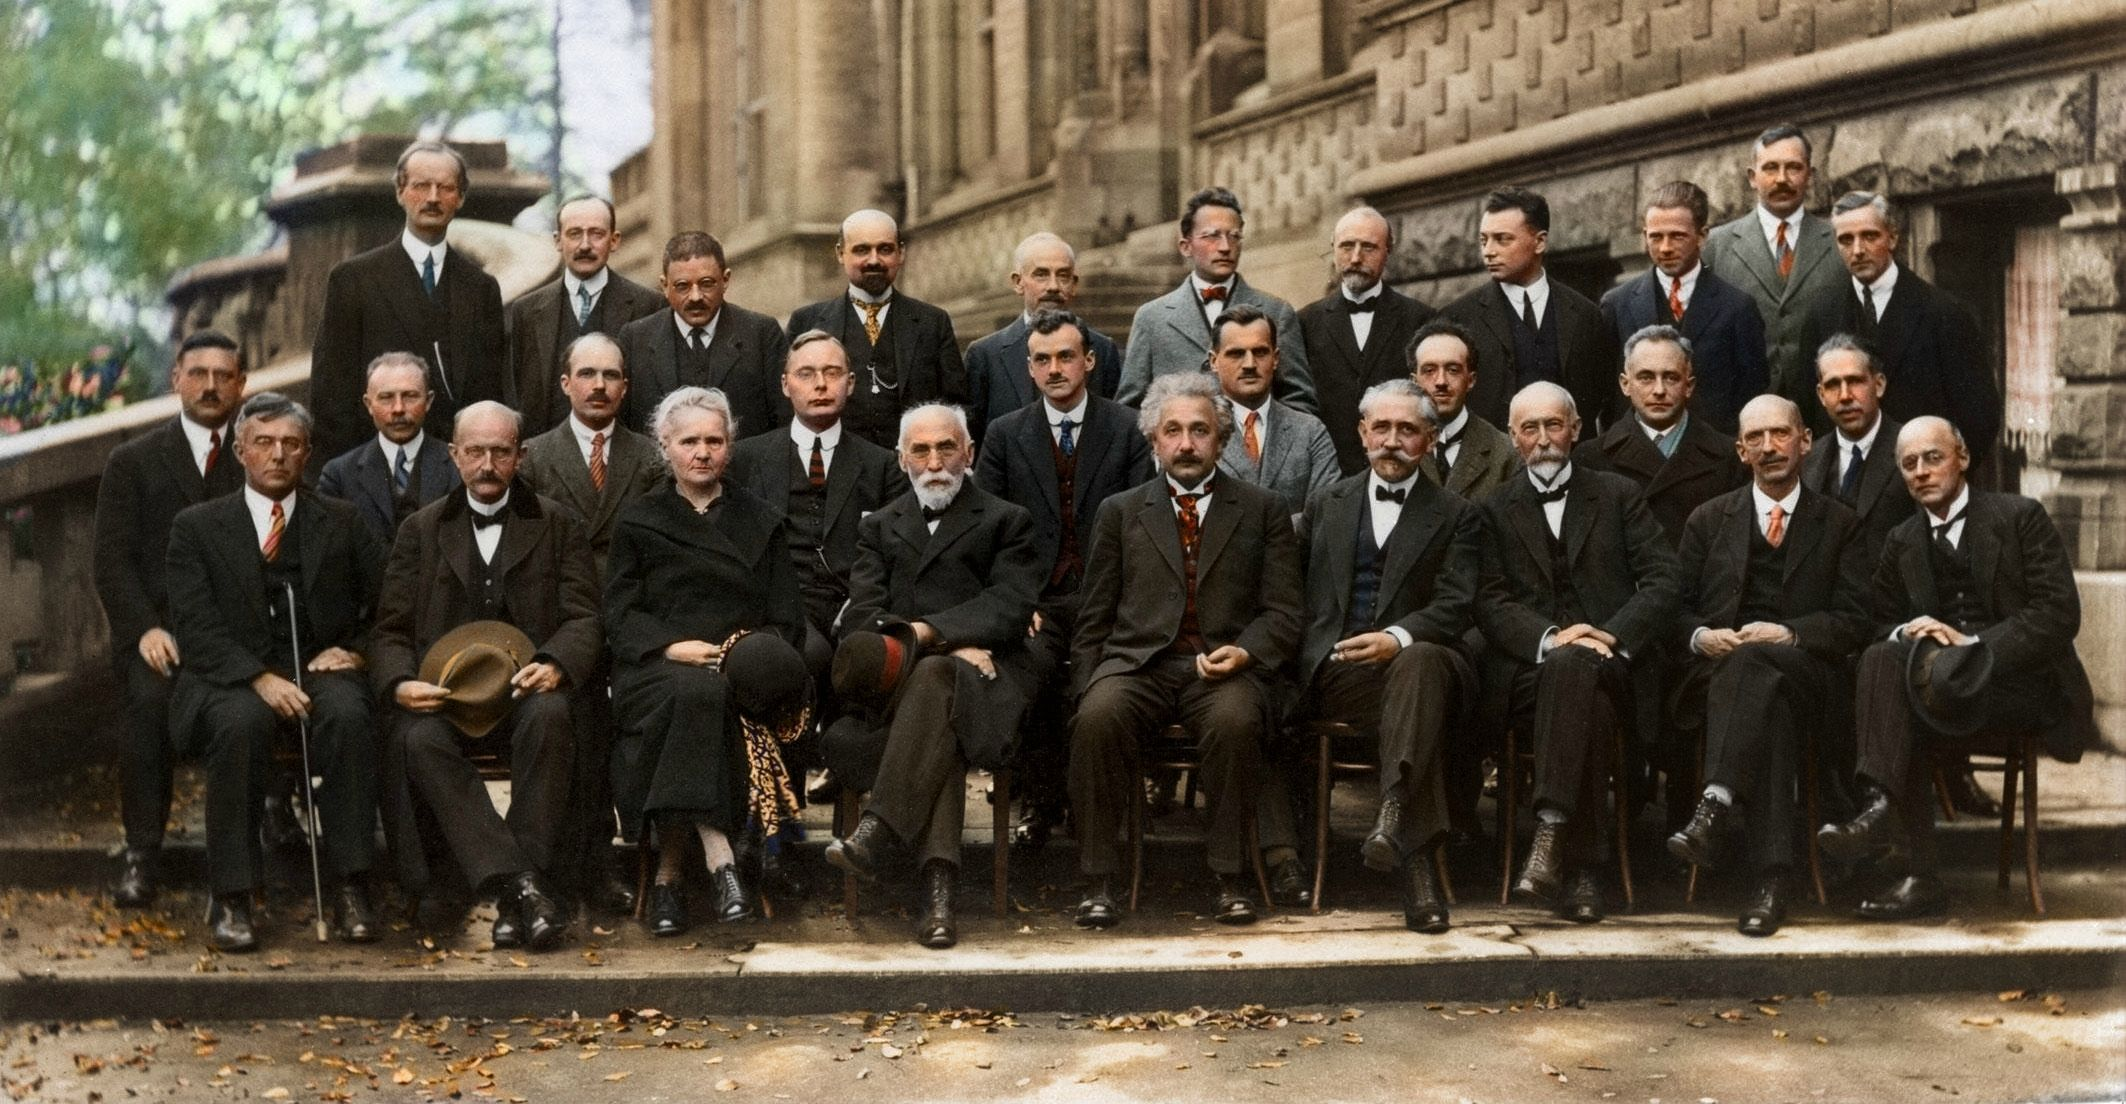
\includegraphics[height=0.57\textwidth,width=1.1\textwidth,viewport=0 0 2150 1050,clip]{Figures/Solvay_Conference-5-fine.jpg}
\vspace{-14.5pt}
\hspace*{-15.5pt}
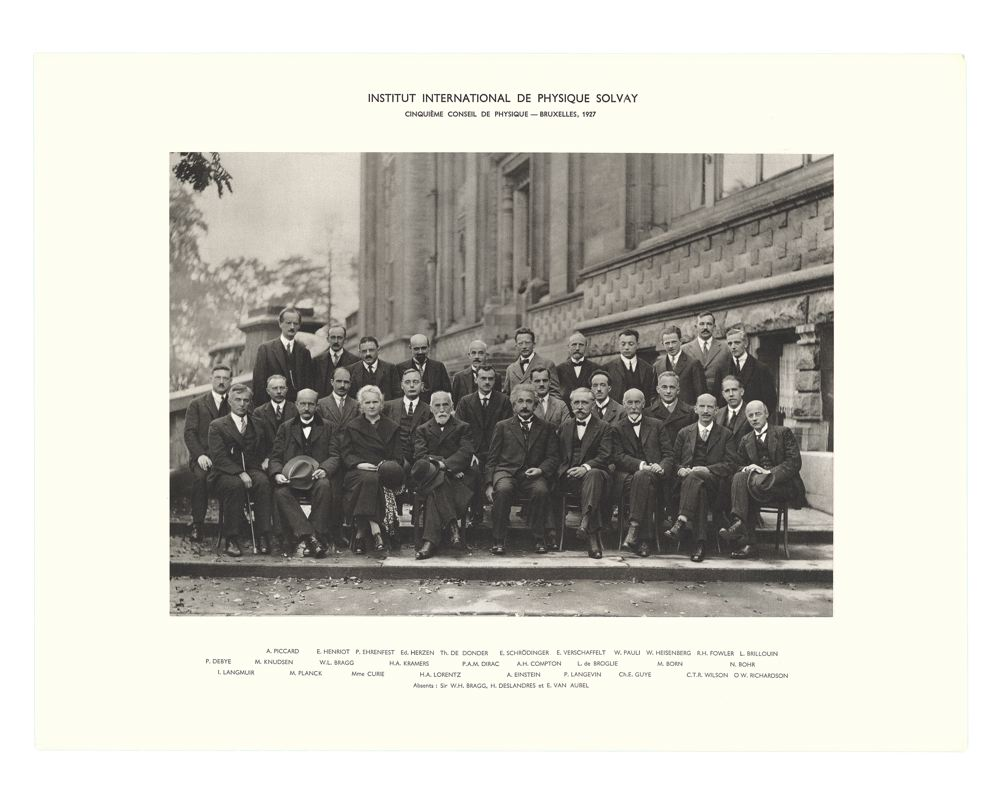
\includegraphics[height=0.58\textwidth,width=0.75\textwidth,viewport=150 105 850 710,clip]{Figures/Solvay_Conference-5.jpg}
\caption{\fontsize{7.5pt}{6.2pt}\selectfont{\textrm{The Fifth Solvay International Conference, Brussels, Belgium, Oct. 1927}}\\
\fontsize{4.1pt}{3.9pt}\selectfont{\textrm{\textcolor{blue}{前排左起}:~I.Langmuir(\textcolor{blue}{朗缪尔}) M.Planck(\textcolor{blue}{普朗克}) Marie Curie(\textcolor{blue}{居里夫人}) H.Lorentz(\textcolor{blue}{洛仑兹}) A.Einstein(\textcolor{blue}{爱因斯坦}) P.Langevin(\textcolor{blue}{朗之万}) Ch.E.Guye(\textcolor{blue}{古伊}) C.T.R.Wilson(\textcolor{blue}{威尔逊}) O.W.Richardson(\textcolor{blue}{理查森})\\
\textcolor{blue}{中排左起}:~P.Debye(\textcolor{blue}{德拜}) M.Knudsen(\textcolor{blue}{克努森}) W.L.Bragg(\textcolor{blue}{布拉格}) H.A.Kramers(\textcolor{blue}{克莱默}) P.A.M.Dirac(\textcolor{blue}{狄拉克}) A.H.Compton(\textcolor{blue}{康普顿}) L.de Broglie(\textcolor{blue}{德布罗意}) M.Born(\textcolor{blue}{玻恩}) N.Bohr(\textcolor{blue}{玻尔})\\
\textcolor{blue}{后排左起}:~A.Piccard(\textcolor{blue}{皮卡尔德}) E.Henriot(\textcolor{blue}{亨利厄特}) P.Ehrenfest(\textcolor{blue}{埃伦费斯特}) Ed.Herzen(\textcolor{blue}{赫尔岑}) Th.de Donder(\textcolor{blue}{德唐德}) E.Schr\"odinger(\textcolor{blue}{薛定谔}) E.Verschaffelt(\textcolor{blue}{费尔夏费尔特}) W.Pauli(\textcolor{blue}{泡利}) W.Heisenberg(\textcolor{blue}{海森堡}) R.H.Fowler(\textcolor{blue}{富勒}) L.Brillouin(\textcolor{blue}{布里渊})}}}
\label{Solvay Conference-5-fine}
\end{figure}
}
%------------------------------------------------------------------------Reference----------------------------------------------------------------------------------------------
\frame
{
	\frametitle{黑体辐射与能量量子化}
	\textrm{1900}年,为了解释黑体辐射\textrm{(black-body radiation)}的能量密度与辐射频率的关系,\textrm{M.~Planck}引入\textcolor{red}{能量量子化}的假设,利用统计物理推导出与实验符合得非常好的黑体辐射\textrm{Planck~}公式:~
	\begin{displaymath}
		\rho_{\nu}\mathrm{d}{\nu}=\dfrac{8{\pi}h{\nu}^3}{C^3}\bigg(\dfrac1{\mathrm{e}^{h\nu/kT}-1}\bigg)\mathrm{d}\nu
	\end{displaymath}
\begin{figure}[h!]
\centering
\vspace{-10.5pt}
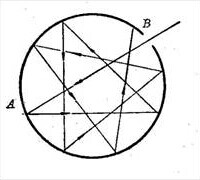
\includegraphics[height=1.5in,width=1.5in,viewport=0 0 136 136,clip]{Figures/Black_box.jpg}
\hskip 1pt
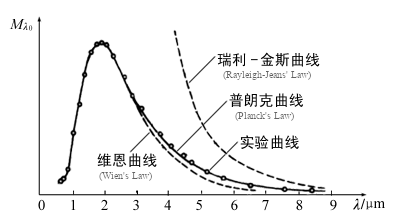
\includegraphics[height=1.5in,width=2.5in,viewport=0 0 390 215,clip]{Figures/Black_box_curve.png}
\caption{\textrm{The black-body radiation and the curve}}
\label{Black_box}
\end{figure}
}

\frame
{
	\frametitle{量子力学基本假设}
	\begin{itemize}
		\item 波函数假设\\
			\textcolor{blue}{微观体系的运动状态可由波函数$\Psi$完全描述,波函数可以得到体系的所有性质}\\
			波函数$\Psi$一般要求满足\textcolor{red}{连续}、\textcolor{red}{有限}和\textcolor{red}{单值}三个条件
		\item 微观体系的运动状态\textcolor{blue}{波函数随时间变化的规律}:\\\textcolor{red}{遵从\textrm{Schr\"odinger}方程}
			$$\mathrm{i}\hbar\dfrac{\mathrm{d}}{\mathrm{d}t}|\Psi\rangle=\hat{\mathbf H}|\Psi\rangle$$
		\item 态叠加原理\\
			如果$\Psi_1$是体系的一个本征态,对应的本征值为$A_1$,$\Psi_2$也是体系的一个本征态,对应的本征值为$A_2$,则\textcolor{blue}{$$\Psi=C_1\Psi_1+C_2\Psi_2$$}\textcolor{red}{也是体系一个可能的存在状态}
	\end{itemize}
}

\frame
{
	\frametitle{Schr\"odinger's cat}
\begin{figure}[h!]
\centering
\vspace{-10.5pt}
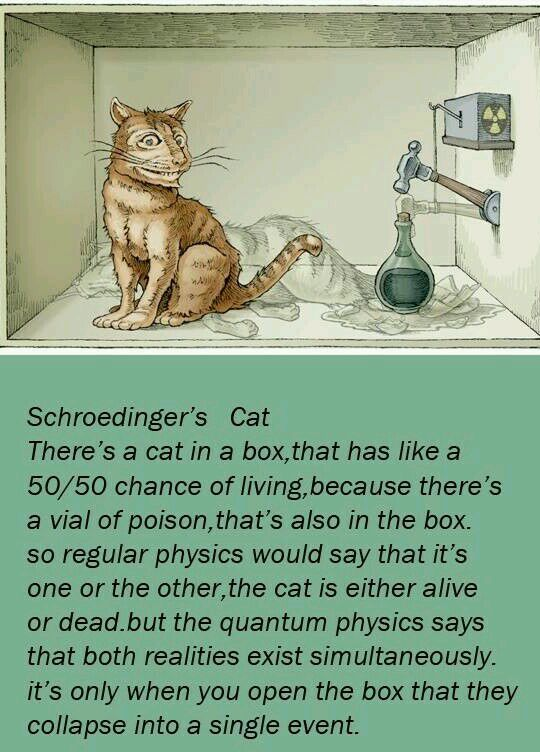
\includegraphics[height=0.70\textwidth,width=0.7\textwidth,viewport=0 0 760 750,clip]{Figures/Schrodinger-cat.jpg}
%\caption{\textrm{ABINIT}的Si.in}
\label{Schrodinger-cat}
\end{figure}
}

\frame
{
	\frametitle{量子力学基本假设}
	\begin{itemize}
		\item 力学量算符假设\\
			\textcolor{blue}{力学量用线性\textrm{Hermite~}算符表示}\\
			在经典力学中的力学量,在量子力学中用力学量的算符表示:\\如动量算符 
			$$\hat{\mathbf{p}}=-\mathrm{i}\hbar\nabla$$
			位置算符$$\hat{\mathbf r}=r$$
			力学量算符之间有确定的对易关系(量子条件)
			$$[\hat{\mathbf F},\hat{\mathbf G}]=\hat{\mathbf F}\hat{\mathbf G}-\hat{\mathbf G}\hat{\mathbf F}$$ 
			\textcolor{red}{\textrm{Hermite~}算符的本征函数构成完备空间}
		\item 全同性原理\\
			\textcolor{blue}{全同粒子组成的体系中,两个全同粒子相互调换不改变体系的状态}\\ 
			全同粒子是指\textcolor{red}{内禀性质完全相同的一类微观粒子}:\\例如,所有的电子是全同粒子 
	\end{itemize}
}

\section{\rm{Hartree-Fock~}方法}
\frame
{
	\frametitle{\textrm{Born-Oppenheimer~}近似}
	\begin{itemize}
		\item 由于原子核的质量要比电子大很多(一般要大3-4个数量级),在同样的相互作用下,原子核的运动比电子也慢得多
		\item 电子在每一时刻仿佛运动在静止原子核构成的势场中,而原子核运动时则感受不到电子的具体位置,感受到的是运动电子的平均作用力
		\item 可近似将原子核坐标与电子坐标变量分离,使得求解整个体系的波函数的复杂过程分解为求解电子波函数和求解原子核波函数两个相对简单的过程\\
			电子运动方程$$\hat{\mathbf H}_{\mathrm e}(\vec r,\vec{\mathbf R})\Psi(\vec r,\vec{\mathbf R})=E_{\mathrm e}(\vec{\mathbf R})\Psi(\vec r,\vec{\mathbf R})$$
			原子核运动方程$$[\hat{\mathbf T}_{\mathrm{nul}}+E_{\mathrm e}(\vec{\mathbf R})]\chi(\vec{\mathbf R})=E\chi(\vec{\mathbf R})$$
	\end{itemize}
}

\frame
{
	\frametitle{独立粒子近似}
	\textrm{n-}粒子体系中的每个粒子的运动,完全忽略粒子间的瞬时相互作用,认为第$i$个粒子在其余$\mathrm{n}-1$个粒子组成的平均势场中运动
	$$\Psi(\vec r_1,\vec r_2,\vec r_3,\cdots,\vec r_n)=\psi_1(\vec r_1)\psi_2(\vec r_2)\psi_3(\vec r_3)\cdots\psi_n(\vec r_n)$$
	$$\hat{\mathbf H}=\sum_{i=1}^N-\dfrac{1}{2}\nabla_i^2+\sum_{i=1}^NV_i(\vec r_i)+\sum_{i,j(j\neq i)}\dfrac{e^2}{|\vec r_i-\vec r_j|}$$
	粒子$i$的\textrm{Hartree}算符
	$$\hat{\mathbf h}_i=-\dfrac{1}{2}\nabla_i^2+V_i(r_i)+\sum_{j(j\neq i)}^N\dfrac{e^2}{|\vec r_i-\vec r_j|}$$
	因此每个粒子的运动方程为:
	$$\hat{\mathbf h}_i\psi_i(\vec r)=\bigg[-\dfrac{1}{2}\nabla_i^2+V_i(r_i)+\sum_{j(j\neq i)}^N\dfrac{e^2}{|\vec r_i-\vec r_j|}\bigg]\psi_i(\vec r)=\varepsilon\psi_i(\vec r)$$ 
}

\frame
{
	\frametitle{\textrm{Slater~}行列式}
	简单乘积的独立粒子波函数不满足全同粒子置换对称性要求,不能正确表示电子不可辨认的物理属性
	
	\textrm{Slater}建议用行列式形式表示具有反对称性的波函数
	\begin{displaymath}
		\hspace*{-10pt}\Psi(\vec r_1,\vec r_2,\vec r_3,\cdots,\vec r_n)=\dfrac1{\sqrt{n!}}
		\left|\begin{array}{ccccc}
			\psi_1(\vec r_1)&\psi_2(\vec r_1)&\psi_3(\vec r_1)&\cdots&\psi_n(\vec r_1)\\
			\psi_1(\vec r_2)&\psi_2(\vec r_2)&\psi_3(\vec r_2)&\cdots&\psi_n(\vec r_2)\\
			\psi_1(\vec r_3)&\psi_2(\vec r_3)&\psi_3(\vec r_3)&\cdots&\psi_n(\vec r_3)\\
			&&&\cdots&\\
			\psi_1(\vec r_n)&\psi_2(\vec r_n)&\psi_3(\vec r_n)&\cdots&\psi_n(\vec r_n)
		\end{array}\right|
	\end{displaymath}
	粒子$i$的\textrm{Fock}算符
	$$\hat{\mathbf F}_i=-\dfrac{1}{2}\nabla_i^2+V_i(r_i)+\hat{\mathbf J}_i-\hat{\mathbf K}_i$$
	$$\hat{\mathbf J}_i(\vec r_i)=\int\dfrac{\psi_j^{\ast}(\vec r_j)|e^2|\psi_j(\vec r_j)}{|\vec r_i-\vec r_j|}\mathrm{d}\vec r_j$$
	$$\hat{\mathbf K}_i(\vec r_i)\psi_i(\vec r_i)=\psi_j(\vec r_i)\int\dfrac{\psi_j(\vec r_j)|e^2|\psi_i(\vec r_j)}{|\vec r_i-\vec r_j|}\mathrm{d}\vec r_j$$

}

\frame
{
	\frametitle{\textrm{Hartree-Fock-Roothan~}方法}
	实际求解非相对论的\textrm{Schr\"odinger}方程时,
	$$\hat{\mathbf F}_i\psi_i(\vec r_i)=\varepsilon_i\psi_i(\vec r_i)$$
	将波函数$\psi_i(\vec r_i)$用一套选定的基函数$\phi_j(\vec r)$展开
	$$\psi_i(\vec r)=\sum_{j=1}^Nc_{ij}\phi_j(\vec r)$$
	通过变分原理
	$$\bar E=\dfrac{\langle\Psi|\hat{\mathbf H}|\Psi\rangle}{\langle\Psi|\Psi\rangle}\geqslant E_0$$
	改变展开系数$c_{ij}$直到体系的能量最小,确定展开系数

	重复上述流程直至\textrm{Fock}算符$\hat{\mathbf F}$、波函数$\psi(\vec r)$和能量$\varepsilon$自洽,这就是\textrm{Hartree-Fock-Roothan}方法
}

\frame
{
	\frametitle{\textrm{RHF~}与\textrm{UHF}} 
	\begin{itemize}
		\item \textrm{RHF}:\\
			针对闭壳层(\textrm{closed shell})体系,占据轨道的电子成对出现,自旋相反,可用一个\textrm{Slater}行列式表示\\
	%		每对自旋相反的电子有相同的轨道波函数\\
			对于闭壳层体系,\textrm{Hartree-Fock}方法求解的能量本征值符合\textrm{Koopmans}定理
			$$E_{ion}^1=-\varepsilon_{\mathrm{HOMO}}$$
		\item \textrm{UHF}:\\
			针对开壳层(\textrm{open shell})体系,占据轨道有未成对电子,需要用\textrm{Slater}行列式的线性组合表示\\
			最低能态用一个\textrm{Slater}行列式,但不同自旋的轨道分别处理
		$$E_{\mathrm{UHF}}\leqslant E_{\mathrm{RHF}}$$
			由于\textrm{UHF}包含更多的变分函数,可以处理一些近解离极限的分子体系
	\end{itemize}
}

\frame
{
	\frametitle{\textrm{Slater~}的$\chi_{\alpha}$方法}
	由于\textrm{Hartree-Fock~}的交换势计算复杂,\textrm{Slater~}建议用电子密度的加权平均来简化交换势的求解
	\begin{displaymath}
		V_{\mathrm x}=-\frac{\sum\limits_i\sum\limits_jn_in_j\int\varphi_i^{\ast}(\vec r)\varphi_i(\vec r{}^{\prime})(2/|\vec r-\vec r{}^{\prime}|)\varphi_j^{\ast}(\vec r{}^{\prime})\varphi_j(\vec r)\mathrm{d}\vec r}{\sum\limits_kn_k\varphi_k^{\ast}(\vec r)\varphi_k(\vec r)}
	\end{displaymath}
	自由电子气在动量空间用\textrm{Hartree-Fock}方法表示
	\begin{displaymath}
		V_{\mathrm x}(k)=-8\left( \frac3{8\pi}\rho \right)^{1/3}F(\eta)
	\end{displaymath}
	这里$\eta=k/k_{\mathrm F}$,并有
	\begin{displaymath}
		F(\eta)=\frac12+\frac{1-\eta^2}{4\eta}\ln\left|\frac{1+\eta}{1-\eta}\right|
	\end{displaymath}
	$F(\eta)$在$\eta=1(k=k_{\mathrm F})$出现奇点(对应于自由电子气\textrm{Fermi~}面上电子密度为0)。
}
	
\frame
{
	\frametitle{\textrm{Slater~}的$\chi_{\alpha}$方法}
	\textrm{Slater~}建议,对占据态($k\leqslant k_{\mathrm F}$)的电子作加权平均,可有
	\begin{displaymath}
		F(\eta)=\frac{\int_0^1\eta^2F(\eta)\mathrm{d}\eta}{\int_0^1\eta^2\mathrm{d}\eta}=\frac34
	\end{displaymath}
	因此,对于均匀电子气,交换势
	\begin{displaymath}
		V_{\mathrm x}=-6\left( \frac3{8\pi}\rho \right)^{1/3}
	\end{displaymath}
	\textrm{Slater~}指出,对于局域电子密度$\rho(\vec r)$体系,可有\textrm{Slater~}交换势
	\begin{displaymath}
		V_{\mathrm xs}(\vec r)=-6\left( \frac3{8\pi}\rho(\vec r) \right)^{1/3}
	\end{displaymath}
	在此基础上,\textrm{Slater~}建议对上述交换势引入可调参数$\alpha$,有交换势
	\begin{displaymath}
		V_{\chi_{\alpha}}(\vec r)=\alpha V_{\mathrm xs}(\vec r)
	\end{displaymath}
}

\frame
{
	\frametitle{交换与相关}
	\begin{itemize}
		\item \textrm{Fock}算符中的交换算符$\hat{\mathrm K}_i(\vec r_i)$是由\textrm{Slater}行列式引入的,属于量子效应
	\end{itemize}
%	\vspace*{-5pt}
	\begin{displaymath}
%		\hspace*{-2pt}
		\text{电子间瞬时相互作用(\textcolor{red}{关联})}
		\left\{
			\begin{aligned}
				&\text{\textcolor{blue}{电子交换}:同自旋电子的关联作用}\\
				&\text{\textcolor{blue}{电子相关}}
			\end{aligned}
			\right.
	\end{displaymath}
\begin{figure}[h!]
\centering
\vspace{-10.5pt}
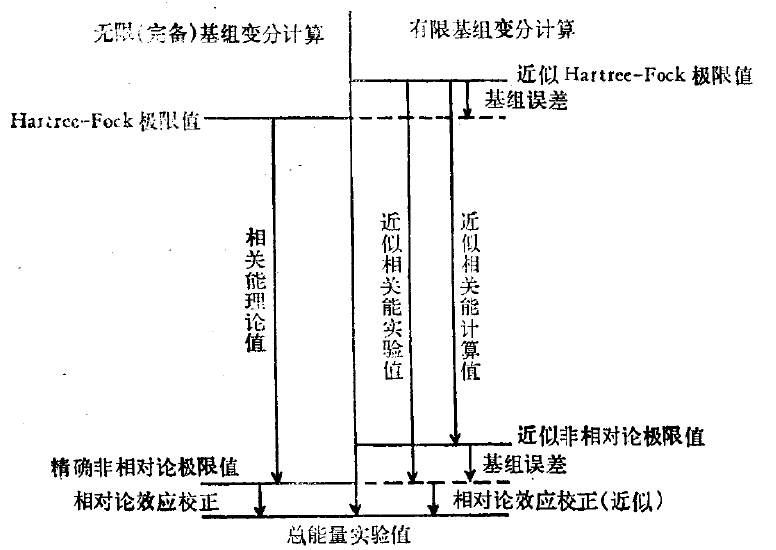
\includegraphics[height=0.42\textwidth,width=0.6\textwidth,viewport=0 0 760 550,clip]{Figures/Post-HF.png}
%\caption{\textrm{ABINIT}的Si.in}
\label{Post-HF}
\end{figure}
}

\frame
{
	\frametitle{\textrm{Post-HF}}
	\textrm{Hartree-Fock}方法精确定义了交换作用,完全没考虑电子相关作用
	\begin{itemize}
		\item \textrm{CI (Configuration Interaction)}
	$$\Psi=\sum_{I=0}C_I\Phi_I=C_0\Phi_0+C_1\Phi_1+C_2\Phi_2+\cdots$$
		\item \textrm{CC (Couple Cluste)}\\
			\begin{displaymath}
				\Psi=\mathrm{e}^{\hat{\mathbf T}}\Phi_0=\mathrm{e}^{(\hat{\mathbf T_1}+\hat{\mathbf T_2}+\hat{\mathbf T_3}+\cdots)}\Phi_0
			\end{displaymath}
		\item \textrm{MP}微扰方法
			\begin{displaymath}
				\begin{aligned}
					&\hat{\mathbf H}=\hat{\mathbf H}^{(0)}+\hat{\mathbf V} \\
					&\hat{\mathbf H}^{(0)}=\sum_i\hat{\mathbf F}_i \qquad \Phi^{(0)}=\Psi_{\mathrm{HF}}\\ 
					&\hat{\mathbf V}=\sum_{j>i}^{occ}\dfrac{e^2}{r_{ij}}-\sum_{ij}^{occ}\big(\hat{\mathbf J}_{ij}-\dfrac12\hat{\mathbf K}_{ij}\big)
				\end{aligned}
			\end{displaymath}
	\end{itemize}
}

\section{密度泛函理论}       %Bookmark
\subsection{\rm{Thomas-Fermi~}模型}       %Bookmark
\frame
{
	\frametitle{\textrm{Thomas-Fermi}模型} 
	1927年,\textrm{Thomas}和\textrm{Fermi}基于均匀电子气模型上建立\textrm{Thomas-Fermi}模型,\textcolor{blue}{体系能量可用}\textcolor{red}{电子密度}\textcolor{blue}{表示}:
	\begin{itemize}
		\item 动能表达式
			$$T_{\mathrm{TF}}[\rho(\vec r)]=\dfrac3{10}(3\pi^2)^{\frac23}\int\rho^{\frac53}(\vec r)\mathrm{d}\vec r$$
		\item 外势$V_{ext}(\vec r)$下电子体系的能量泛函表达式为
			\begin{displaymath}
				\begin{aligned}
					E_{\mathrm{TF}}[\rho(\vec r)]=&\dfrac3{10}(3\pi^2)^{\frac23}\int\rho^{\frac53}(\vec r)\mathrm{d}\vec r\\
					&+\int\rho(\vec r)V_{ext}(\vec r)\mathrm{d}\vec r+\dfrac12\int\int\dfrac{\rho(\vec r_1)\rho(\vec r_2)}{|\vec r_2-\vec r_1|}\mathrm{d}\vec r_1\mathrm{d}\vec r_2
				\end{aligned}
			\end{displaymath}
		\item \textrm{Thomas-Fermi}模型完全没有考虑电子的交换-相关作用
	\end{itemize}
}

\frame
{
	\frametitle{\textrm{Thomas-Fermi-Dirac}模型} 
	1930年,\textrm{Dirac}将\textrm{Thomas-Fermi}模型修正,用局域密度近似考虑电子交换作用
			\begin{displaymath}
				\begin{aligned}
					E_{\mathrm{TFD}}[\rho(\vec r)]=&\dfrac3{10}(3\pi^2)^{\frac23}\int\rho^{\frac53}(\vec r)\mathrm{d}\vec r+\int\rho(\vec r)V_{ext}(\vec r)\mathrm{d}\vec r\\
					&+\dfrac12\int\int\dfrac{\rho(\vec r_1)\rho(\vec r_2)}{|\vec r_2-\vec r_1|}\mathrm{d}\vec r_1\mathrm{d}\vec r_2-\dfrac34\bigg(\dfrac3{\pi}\bigg)^{\frac13}\int\rho^{\frac43}(\vec r)\mathrm{d}\vec r
				\end{aligned}
			\end{displaymath}
			\begin{itemize}
				\item 在总电子数守恒约束条件
					$$\int\rho(\vec r)\mathrm{d}\vec r=N$$
					下,能量泛函$E_{\mathrm{TFD}[\rho(\vec r)]}$对密度$\rho(\vec r)$的变分极小获得体系的基态密度和基态能量
			\end{itemize}
}

\frame
{
	\frametitle{\textrm{Thomas-Fermi}模型}
	\begin{itemize}
		\item \textrm{Thomas-Fermi}模型用电子密度代替波函数描述问题是极大的简化,但模型过于粗糙:\\
%			\begin{enumerate}
%				\item 以均匀电子气的密度得到动能的表达式
%				\item 完全忽略电子间的交换-相关作用
%			\end{enumerate}
			不能正确描述相互作用电子体系的基本特征,如原子的壳层结构
		\item \textrm{Thomas-Fermi}模型虽不够精确,但可以通过引入修正项校正:
			\textrm{Dirac}交换泛函 $$E_X[\rho(\vec r)]=-\dfrac34\bigg(\dfrac3{\pi}\bigg)^{\frac13}\int\rho^{\frac43}(\vec r)\mathrm{d}\vec r$$
			\textrm{Wigner}相关泛函 $$E_C[\rho(\vec r)]=-0.056\int\dfrac{\rho^{\frac43}(\vec r)}{0.079+\rho^{\frac13}(\vec r)}\mathrm{d}\vec r$$
	\end{itemize}
	\textrm{Thomas-Fermi}模型为密度泛函理论\textrm{(DFT)}提供了重要的启示
}

\subsection{密度泛函理论}       %Bookmark
\frame                               %
{
\frametitle{密度泛函理论(\textrm{DFT})} %Slide Page Title
%   \secname
与传统的量子力学方法不同,密度泛函理论的基本变量是体系的基态电子密度。%通过体系的电子密度而非波函数确定体系的基态能量。
\begin{itemize}%[+-| alert@+>]
	\item 密度泛函理论的基石:\textrm{Hohenberg-Kohn}定理\upcite{PR136-B864_1964}
\vskip 5pt
\begin{itemize}%[+-| alert@+>]
   \setlength{\itemsep}{8pt}
 \item $E[\rho]=F_{\mathrm{HK}}[\rho]+\displaystyle\int\rho(\vec{r})v(\vec{r})\textrm{d}\vec{r}$ \\
\vskip 5pt 其中$F_{\mathrm{HK}}[\rho]=\underset{\Psi\to\rho}{\mathrm{Min}}\langle\Psi[\rho]|\hat{T}+\hat{W}|\Psi[\rho]\rangle$
是普适的泛函表达式。%,指明多电子体系的基态性质与基态密度间存在一一对应关系
     \textrm{\small{第一定理表明多电子体系的性质完全由体系的基态密度决定}}
   \item 如果$\tilde\Psi\neq\Psi$,
     $E[\tilde\rho]\geqslant E[\rho_0]$\\
     \textrm{\small{第二定理指出基态总能量泛函在体系基态电子密度处取极小值}}
   \end{itemize}
%\textrm{\small{第二定理指出基态总能量泛函在体系基态电子密度处取极小值}}
\vskip 8pt
 \item 密度泛函理论的优越性:用密度($\rho$)代替波函数($\Psi$)描述体系
\vskip 5pt
 \item 密度泛函理论的困难:能量密度泛函的精确形式未知
   \end{itemize}
}
\frame                               %
{
\frametitle{密度泛函理论(\textrm{DFT})}
\textrm{Kohn-Sham}方程\upcite{PR140-A1133_1965}:无相互作用体系+交换-相关能
$$(T_S+V_{e\!f\!f})|\varphi_i\rangle=\varepsilon_i|\varphi_i\rangle,\quad i=1,\cdots,N,\cdots$$
其中$V_{e\!f\!f}(\vec r)=v(\vec r)+\displaystyle\int w(\vec r,\vec r\,')\rho(\vec r\,')\mathrm{d}\vec r+\dfrac{\delta E_{XC}}{\delta\rho(\vec r)}$
\vskip 10pt
\textrm{Kohn-Sham}方程是形式上的单粒子方程
\vskip 20pt
\textrm{Kohn-Sham}方程的实质:\\\textcolor{red}{将动能泛函的主要部分分离出来,剩余部分放在交换-相关能中}
}
%  \beamertemplateshadingbackground{blue!10}{yellow!10}
\frame                               %
{
\frametitle{交换-相关能密度泛函}
\begin{minipage}[b]{0.72\linewidth}
 \hspace*{-15pt}
 \begin{itemize}%[+-| alert@+>]
	 \setlength{\itemsep}{10pt}
 \item \textrm{LDA}:泛函只与密度分布的局域值有关
 \item \textrm{GGA}:泛函依赖:局域密度及其梯度
 \item $meta$-\textrm{GGA}:泛函依赖的变量还有动能密度
 \item 杂化(\textrm{hybrid})泛函:泛函与占据轨道有关
 \item 其他的交换-相关能泛函
 \item<1-> 完全非局域泛函:理想泛函,不现实
 \end{itemize}
\end{minipage}
\hfill
\begin{minipage}[b]{0.26\linewidth}
\hspace*{-10pt}
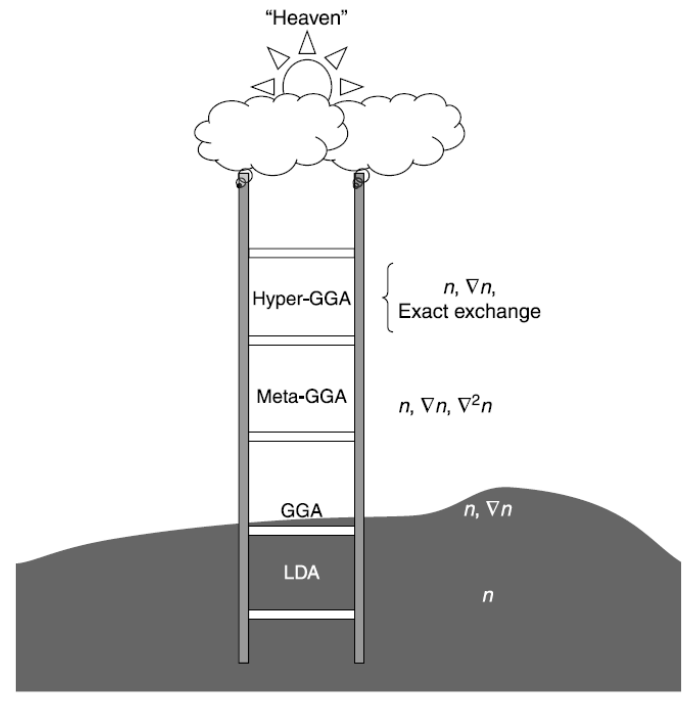
\includegraphics[height=1.7in,width=3.18in,viewport=10 5 1380 700,clip]{Figures/Jacobi-ladder.png}\\
{\small \textcolor{red}{\textrm{Jacob's ladder}}}
\end{minipage}
% \begin{itemize}%[+-| alert@+>]
%\item 交换-相关能密度泛函
}

\frame                               %
{
	\frametitle{近似能量泛函$E_{\mathrm{XC}}[\rho]$的主要问题}
\vskip 20pt
\begin{enumerate}%[+-| alert@+>]
   \setlength{\itemsep}{30pt}
 \item  密度是整体变量:~电子自相互作用抵消不净%\quad\textrm{(LDA+U)}方法的校正%(\textrm{LDA+U})
 \item  电子相关:~简并和近简并基态的表示不合理
 \item  渐近行为:~处理弱相互作用体系的误差大
 \end{enumerate}
}

\frame                               %
{
	\frametitle{\textrm{Kohn-Sham}方程}
\begin{figure}[h!]
\centering
\vspace*{-0.21in}
\hspace*{-0.1in}
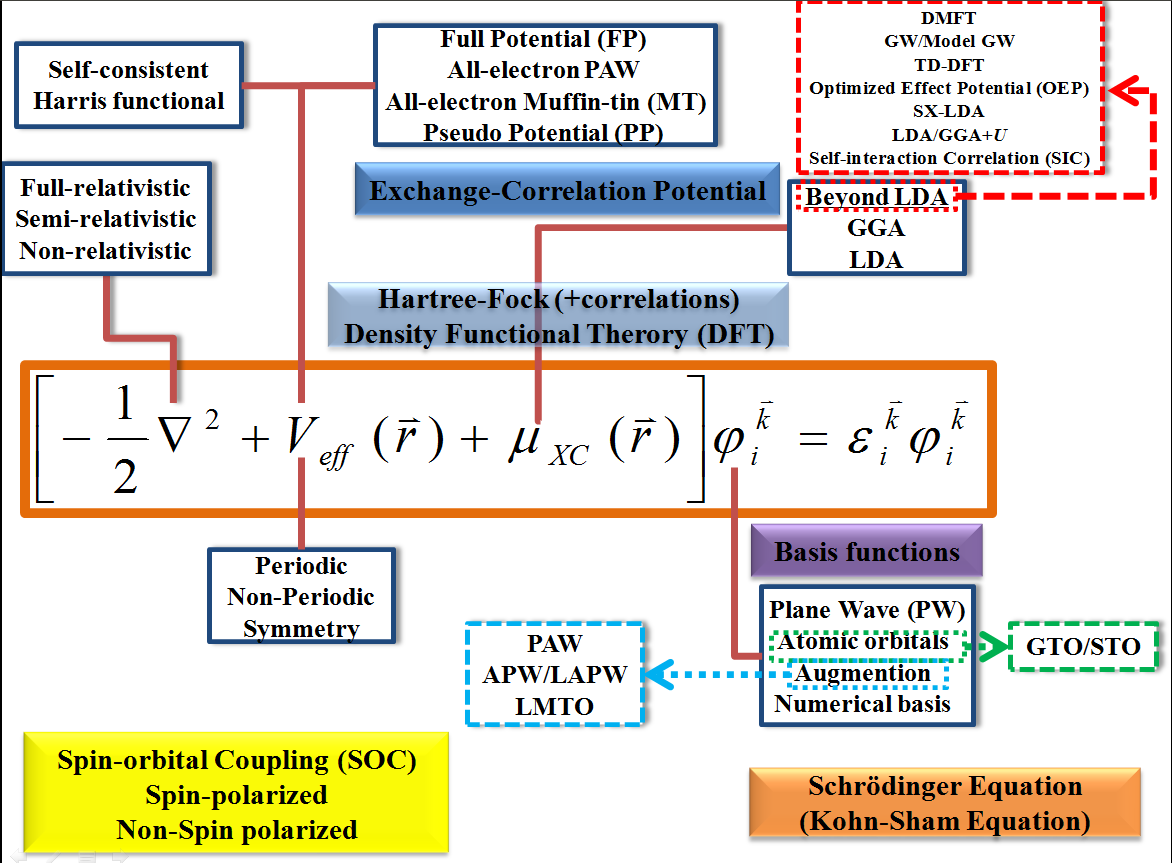
\includegraphics[height=2.7in,width=4.0in,viewport=2 5 1162 880,clip]{Figures/DFT.png}
\caption{\small \textrm{The Analysis of Kohn-Sham equation.}}%(与文献\cite{EPJB33-47_2003}图1对比)
\label{DFT}
\end{figure}
}

\section{固体能带理论}       %Bookmark
\frame
{
%\frametitle{The Bloch theorem}
	\frametitle{\textrm{Bloch~}定理}
\begin{itemize}%[+-| alert@+>]
   \setlength{\itemsep}{8pt}
   \item 固体能带理论\upcite{Huang_Han}是固体电子理论的基础,形式上是单电子理论:
    $$\hat H |\psi_i^{\vec k}(\vec r)\rangle=\bigg[-\dfrac{\hbar^2}{2m}\nabla^2+V(\vec r)\bigg]|\psi_i^{\vec k}(\vec r)\rangle=\epsilon_i(\vec k)|\psi_i^{\vec k}(\vec r)\rangle$$
  \item \textrm{Bloch}定理:
%   \item \textrm{periodic potential:} $$V(\vec r)=V(\vec r+\vec R_n)$$
%     \textrm{Here,} $\vec R_n=n\vec R$
%   \item \textrm{Bloch theorem:}$$\psi_{\vec k}(\vec r)=\textrm{e}^{\textrm i\vec k\cdot\vec r}u_{\vec k}(\vec r)$$
%     \textrm{Here, $u_{\vec k}(\vec r)$ is a periodic function with the same periodicity as $V(\vec r)$, i.e., $u_{\vec k}(\vec r)=u_{\vec k}(\vec r+\vec R_n)$, then Bloch theorem could reads as:}
%     $$\psi_{\vec k}(\vec r+\vec R_n)=\textrm{e}^{\textrm i\vec k\cdot\vec R_n}\psi_{\vec k}(\vec r)$$
具有平移周期性的理想晶体,势能$V(\vec r)$满足$$V(\vec r)=V(\vec r+\vec R_n)$$
体系的波函数满足\textrm{Bloch}波函数形式:$$\psi_{\vec k}(\vec r)=\textrm{e}^{i\vec k\cdot\vec r}u_{\vec k}(\vec r)$$
是平面波和周期函数的乘积。$u(\vec r)$与势能有相同的周期。即$$u_{\vec k}(\vec r)=u_{\vec k}(\vec r+\vec R_n)$$
  \item 能带理论相当于分子轨道理论
%   \setlength{\itemsep}{30pt}
\item \textrm{Bloch}函数反映了波函数在周期性势场下的变化规律。
\end{itemize}
}

\frame
{
\frametitle{周期体系的波函数}
物质的电子体系,可分为芯层分子和价层电子。芯电子能量低,受周围化学环境影响很小,基本保持原子属性;价层电子相互作用较强,对化学环境较为敏感。一般地,价电子波函数在原子间区域(\textrm{Interstitial}区)的变化平缓,在临近原子核附近区域(\textrm{Muffin-tin}球内),会出现剧烈振荡(与芯层波函数正交)。
\begin{figure}[h!]
\centering
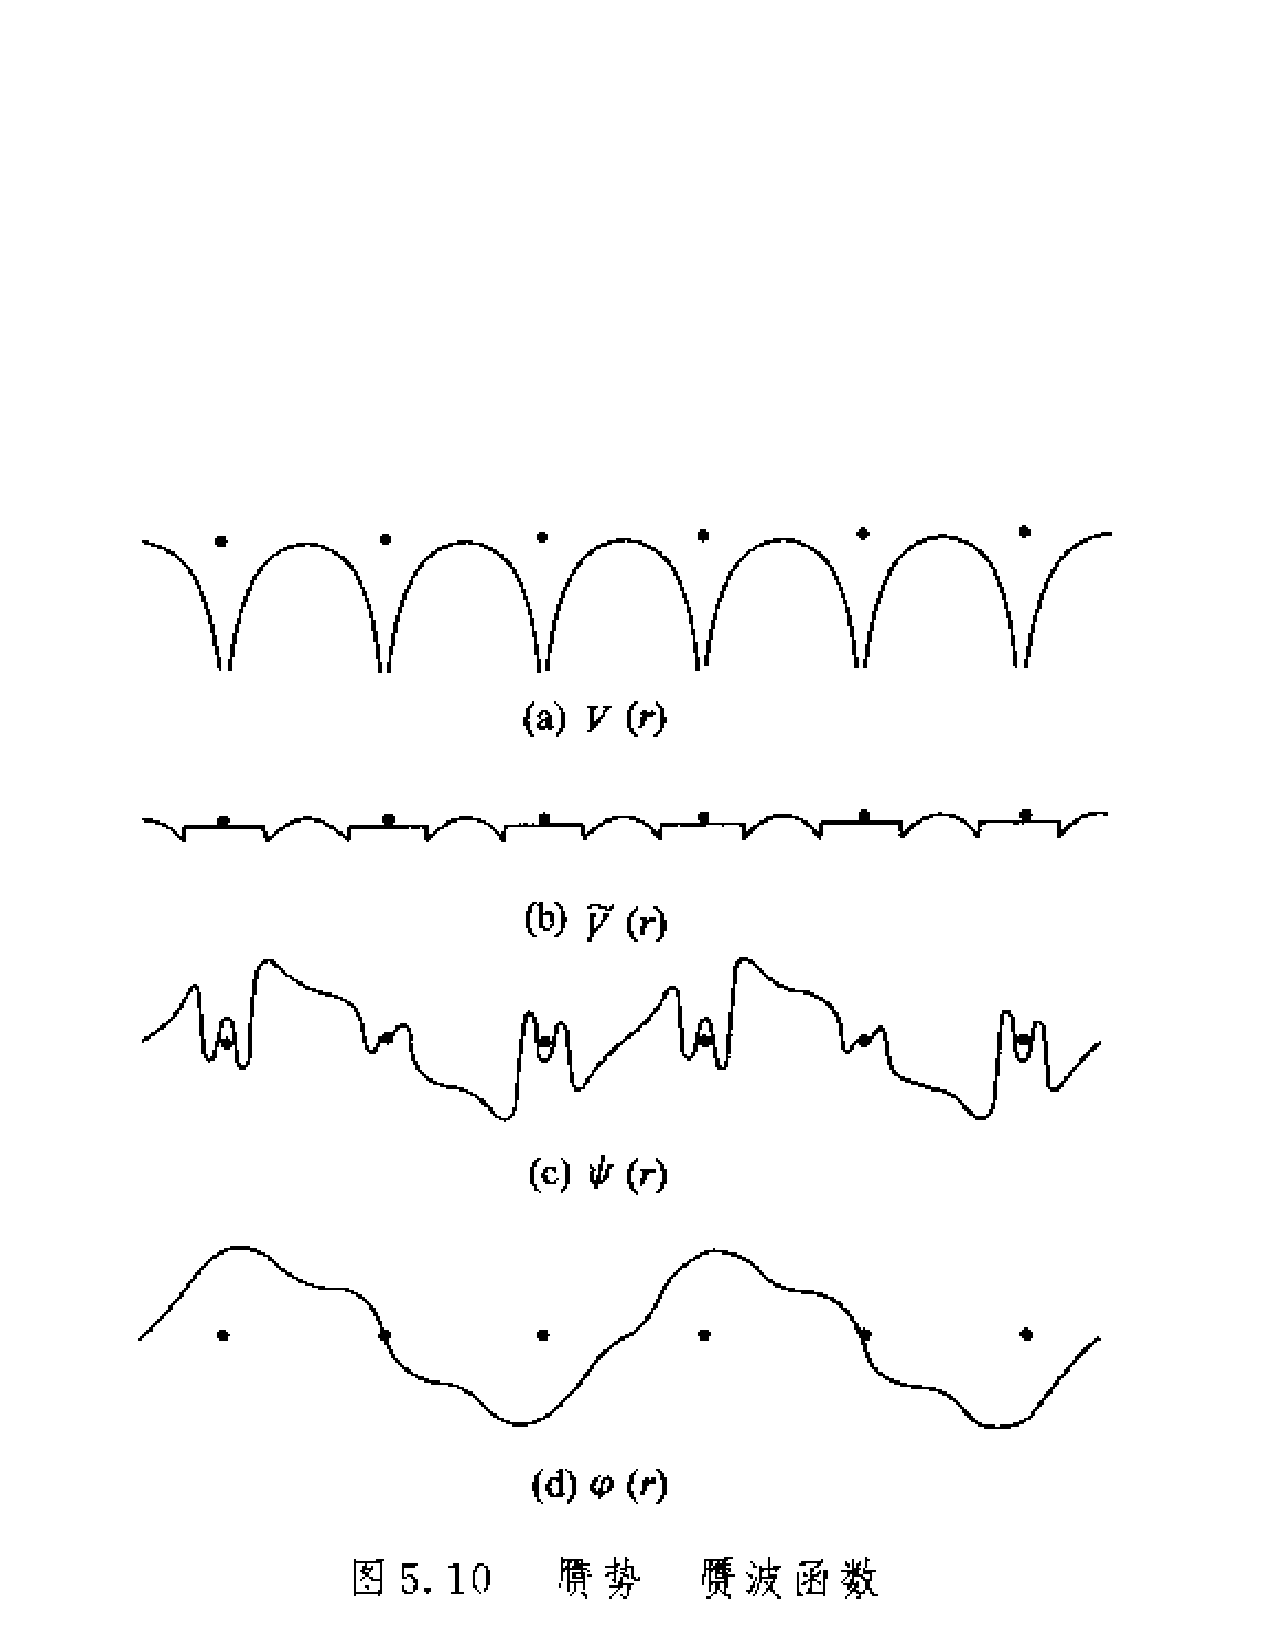
\includegraphics[height=0.8in,width=4.in,viewport=41 433 539 546,clip]{Figures/Pseudo_wave.pdf}\\
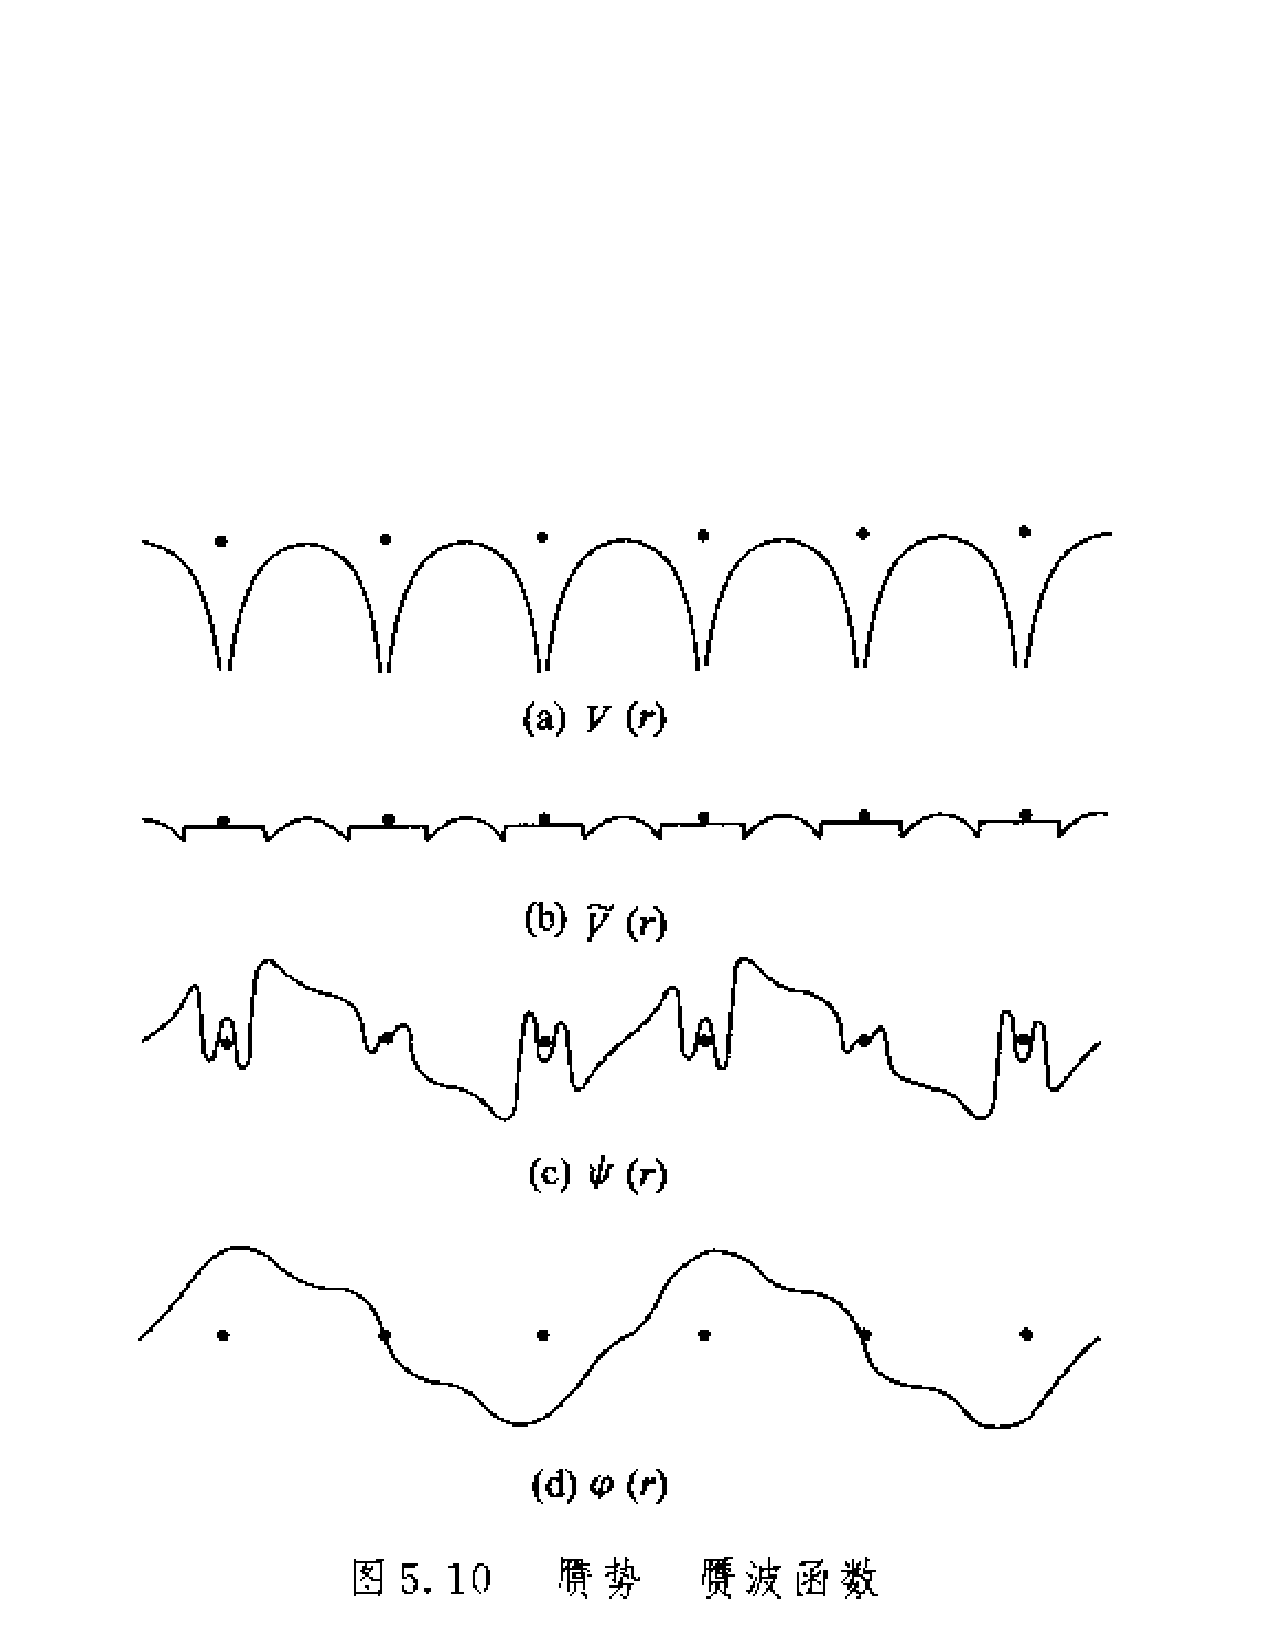
\includegraphics[height=0.8in,width=4.in,viewport=41 210 539 339,clip]{Figures/Pseudo_wave.pdf}
\caption{\small \textrm{The periodic Potential and the wave functions in crystal.}}%(与文献\cite{EPJB33-47_2003}图1对比)
\label{Potential-Wave}
\end{figure}
}

\frame
{
\frametitle{一维自由电子近似微扰}
\begin{figure}[h!]
\centering
%\hspace*{-10pt}
%\vspace*{-1.1in}
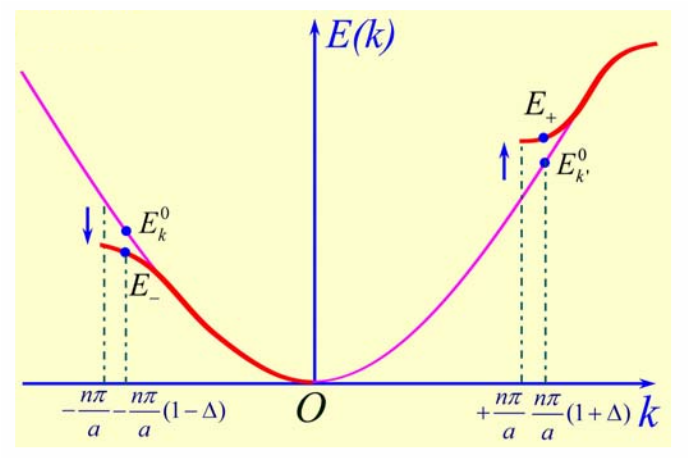
\includegraphics[height=1.5in,width=2.5in,viewport=5 5 700 450,clip]{Figures/Band_Gap-2.png}
%\caption{\small \textrm{The Band-structure from free-electron gas.}}%
\label{Band-Gap-1}
\end{figure} 
\begin{displaymath}
	\begin{aligned}
		&\hat H_0=-\dfrac{\hbar^2}{2m}\dfrac{\mathrm{d}^2}{\mathrm{d}x^2}+\={V} \longrightarrow \hat H=\hat H_0+\hat H^{\prime}=-\dfrac{\hbar^2}{2m}\dfrac{\mathrm{d}^2}{\mathrm{d}x^2}+\={V}+\underline{V(x)-\={V}}\\
		&\Psi_k^0(x)=\dfrac1{\sqrt V}\mathrm{e}^{\mathrm{i}k\cdot x} \longrightarrow \Psi_k(x)=\Psi_k^0(x)+\sum_{k^{\prime}\neq k}\dfrac{\langle k^{\prime}|\hat H^{\prime}|k\rangle}{E_k^0-E_{k^{\prime}}^0}\Psi_{k^{\prime}}^0(x)\\
		&\hat E_k^0=-\dfrac{\hbar^2k^2}{2m}+\={V} \longrightarrow E_k=%E_k^0+E^{\prime}=
		\dfrac{\hbar^2k^2}{2m}+\={V}+\sum_n{}^{\prime}\dfrac{|V_n|^2}{\frac{\hbar^2}{2m}[k^2-(k+2\pi\frac na)^2]}
	\end{aligned}
\end{displaymath}
}

\frame
{
\frametitle{一维自由电子简并微扰}
在波矢$k=\pm\frac{n\pi}{a}$位置,电子能量出现简并态,必须采用简并态微扰理论处理
\begin{figure}[h!]
\centering
%\hspace*{-10pt}
%\vspace*{-1.1in}
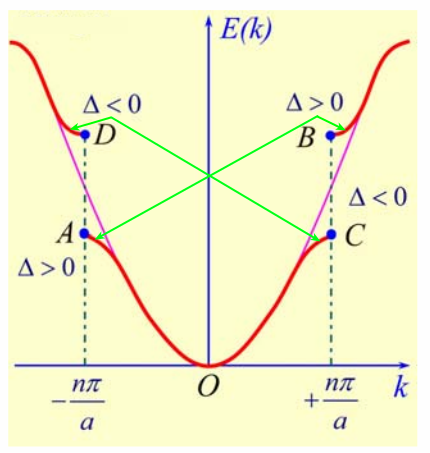
\includegraphics[height=1.3in,width=1.4in,viewport=0 5 420 450,clip]{Figures/Band_Gap-1.png}
%\caption{\small \textrm{The Band-structure from free-electron gas.}}%
\label{Band-Gap-1}
\end{figure} 
\begin{displaymath}
	E_{\textcolor{red}{\pm}}=\left\{
	\begin{aligned}
		&T_n+\={V}\textcolor{red}{+}\Delta^2T_n\bigg(\dfrac{2T_n}{|V_n|}\textcolor{red}{+}1\bigg)\\
		&T_n+\={V}\textcolor{red}{-}\Delta^2T_n\bigg(\dfrac{2T_n}{|V_n|}\textcolor{red}{-}1\bigg)
	\end{aligned}\right.
\end{displaymath}
这里$T_n=\frac{\hbar^2}{2m}\big(\frac{n\pi}a\big)^2$
}

\frame
{
\frametitle{自由电子气模型}
简并态微扰理论引起的能带裂分
\begin{figure}[h!]
\centering
%\hspace*{-10pt}
%\vspace*{-1.1in}
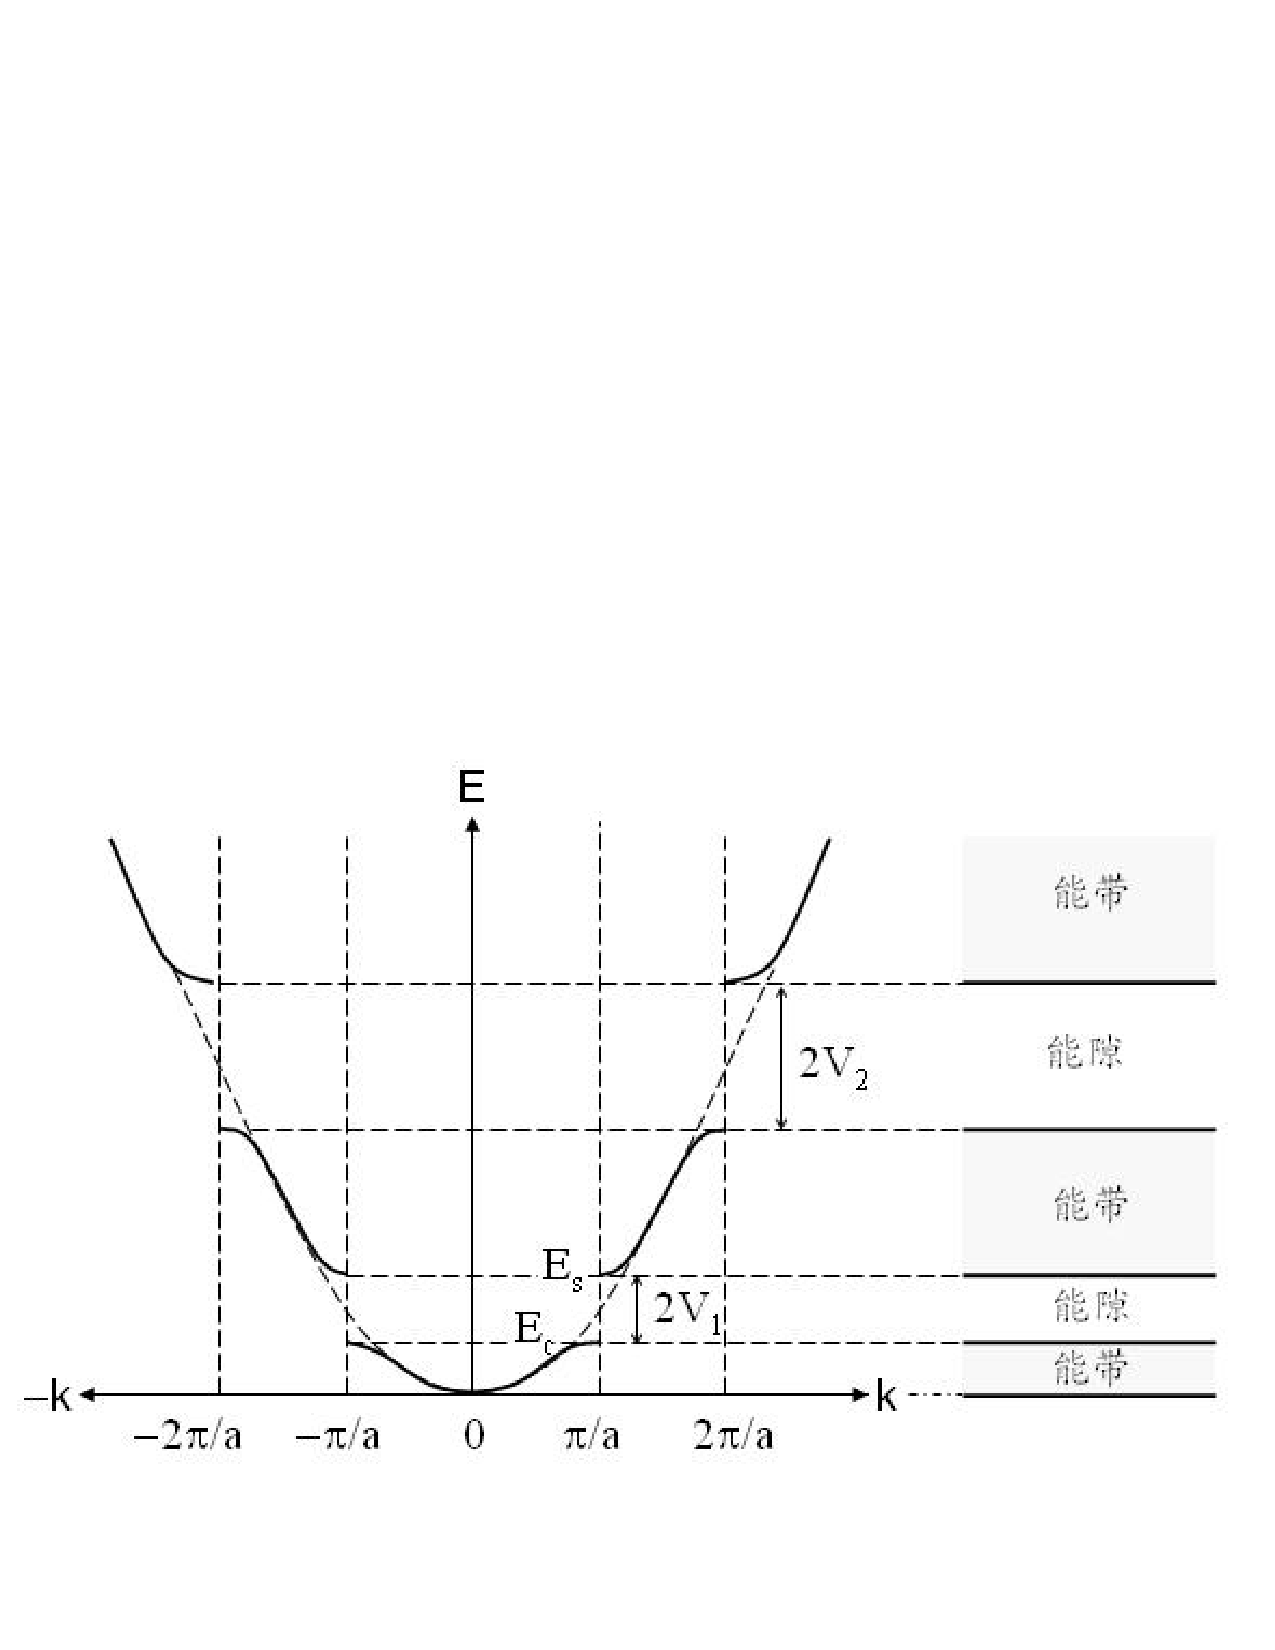
\includegraphics[height=2.1in,width=3.8in,viewport=10 90 570 380,clip]{Figures/Band_Gap.pdf}
\caption{\small \textrm{The Band-structure from free-electron gas.}}%
\label{Band-Structure-1}
\end{figure} 
}

\frame
{
\frametitle{紧束缚模型}
从分子轨道到能带
\begin{figure}[h!]
\centering
\hspace*{-0.29in}
\vspace*{-0.1in}
\subfigure[一维$\mathrm{H}$原子链]{
\label{fig:Hydrogen-1D}
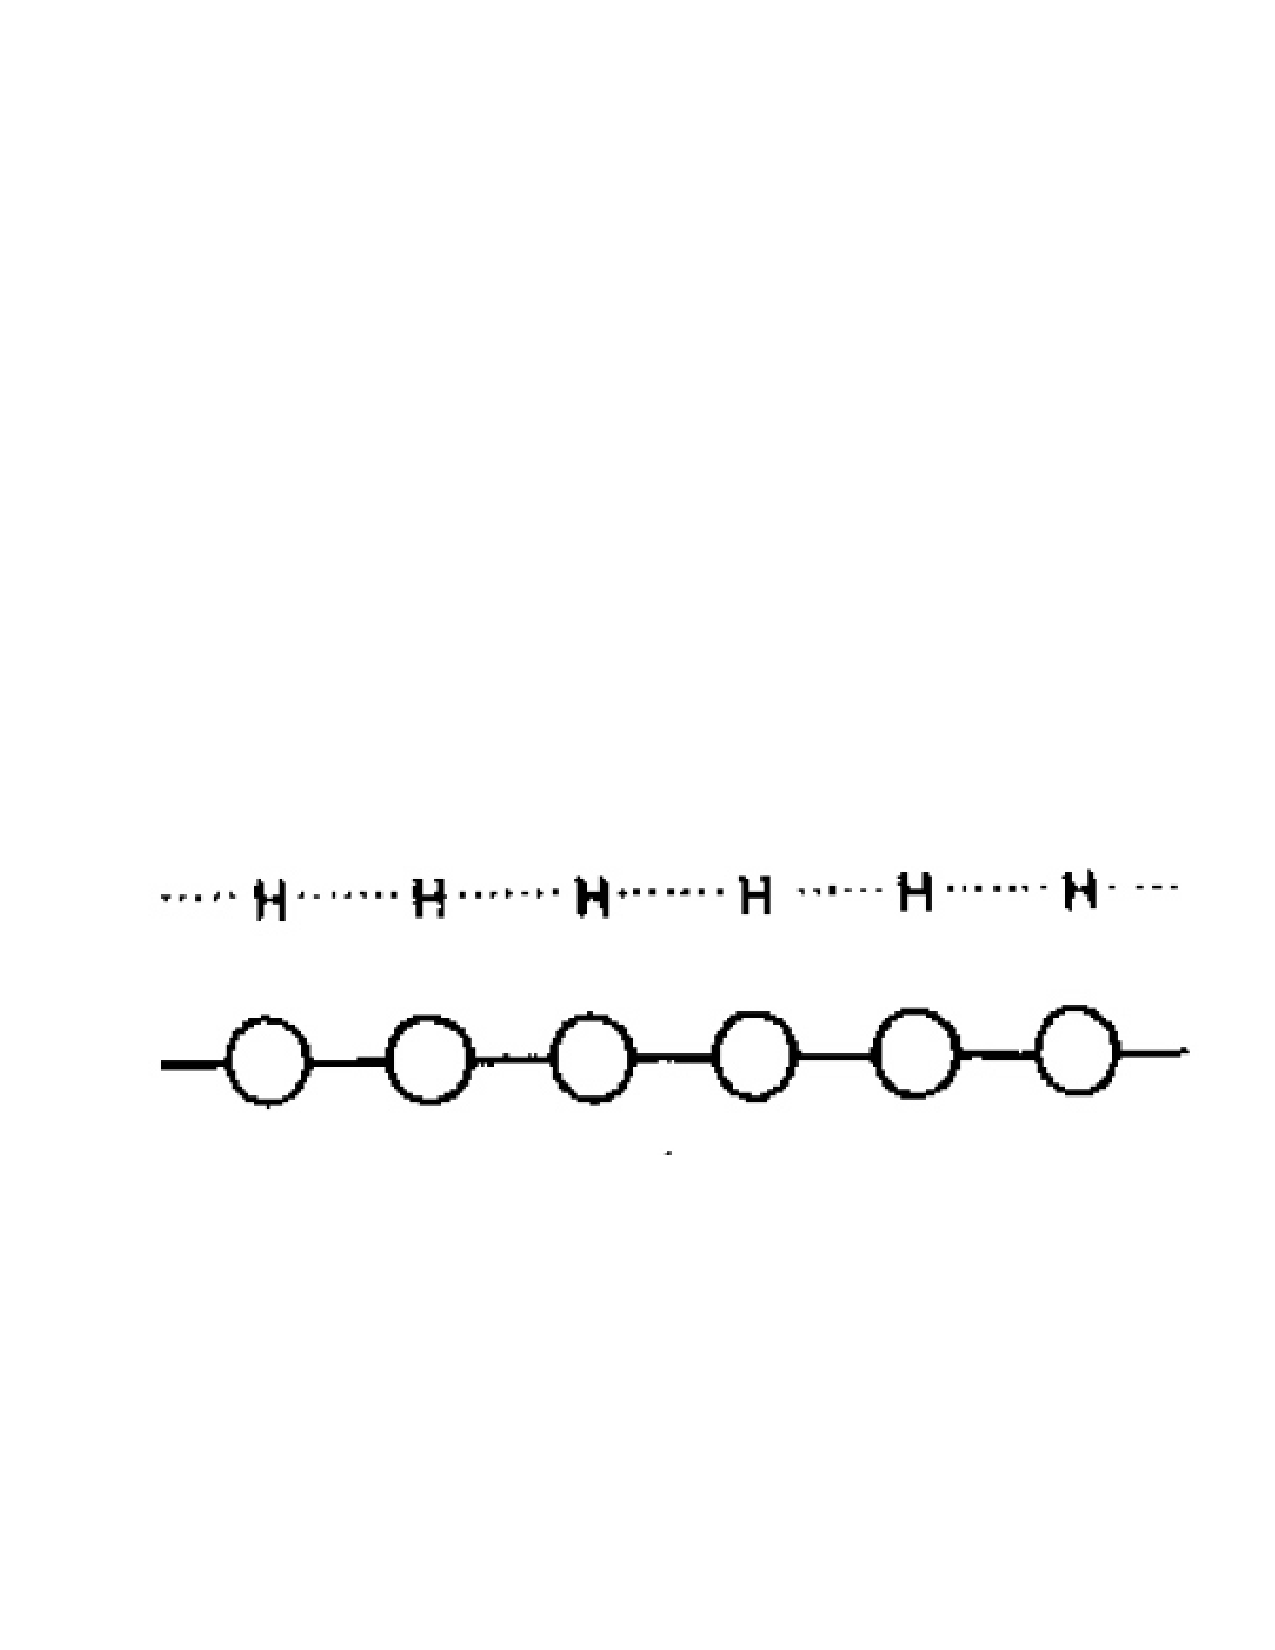
\includegraphics[height=0.25in,width=1.1in,viewport=70 255 570 375,clip]{Figures/Hydrogen-1D.pdf}}
\subfigure[$\mathrm{H}_n$分子轨道]{
\label{fig:Hydrogen-2-n}
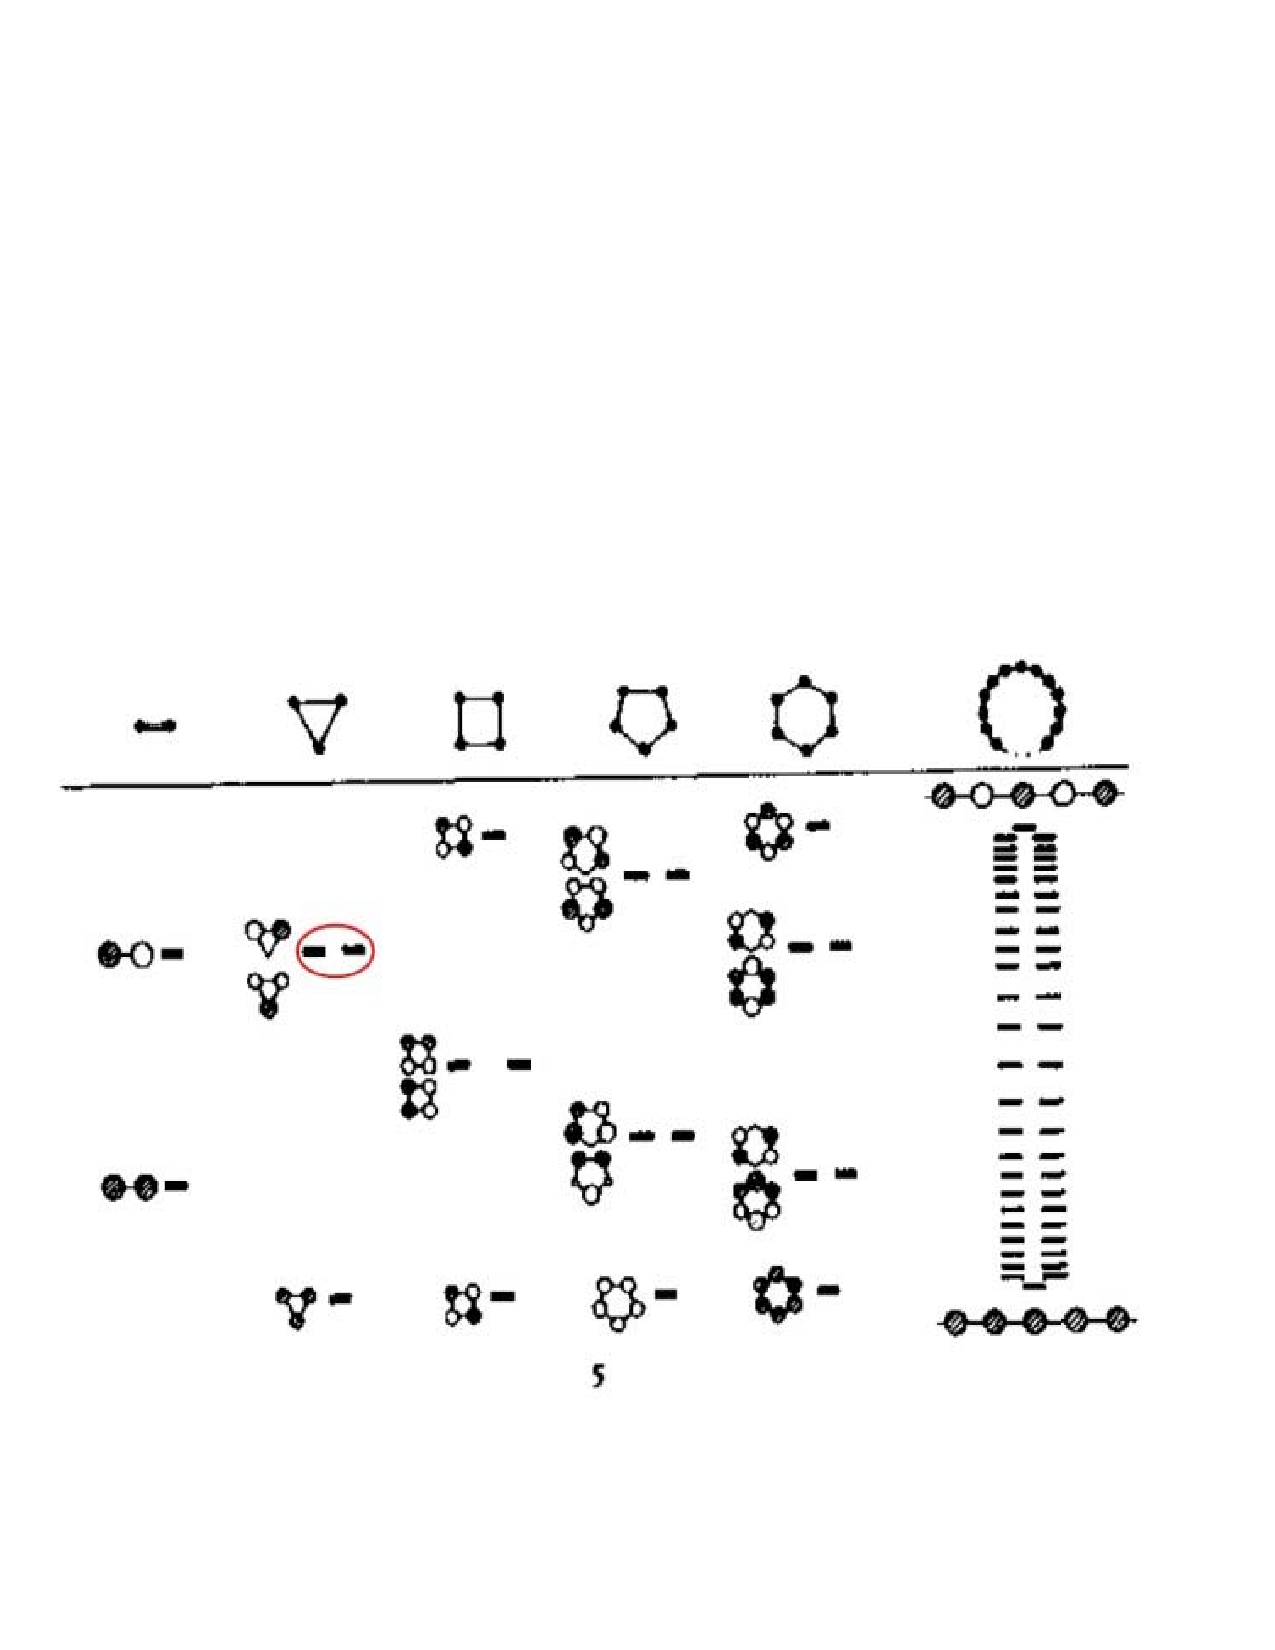
\includegraphics[height=0.8in,width=1.5in,viewport=30 140 545 480,clip]{Figures/Hydrogen-Mol-Orbital.pdf}}
\subfigure[分子波函数]{
\label{fig:Hydrogen-Psi}
\vspace*{-0.2in}
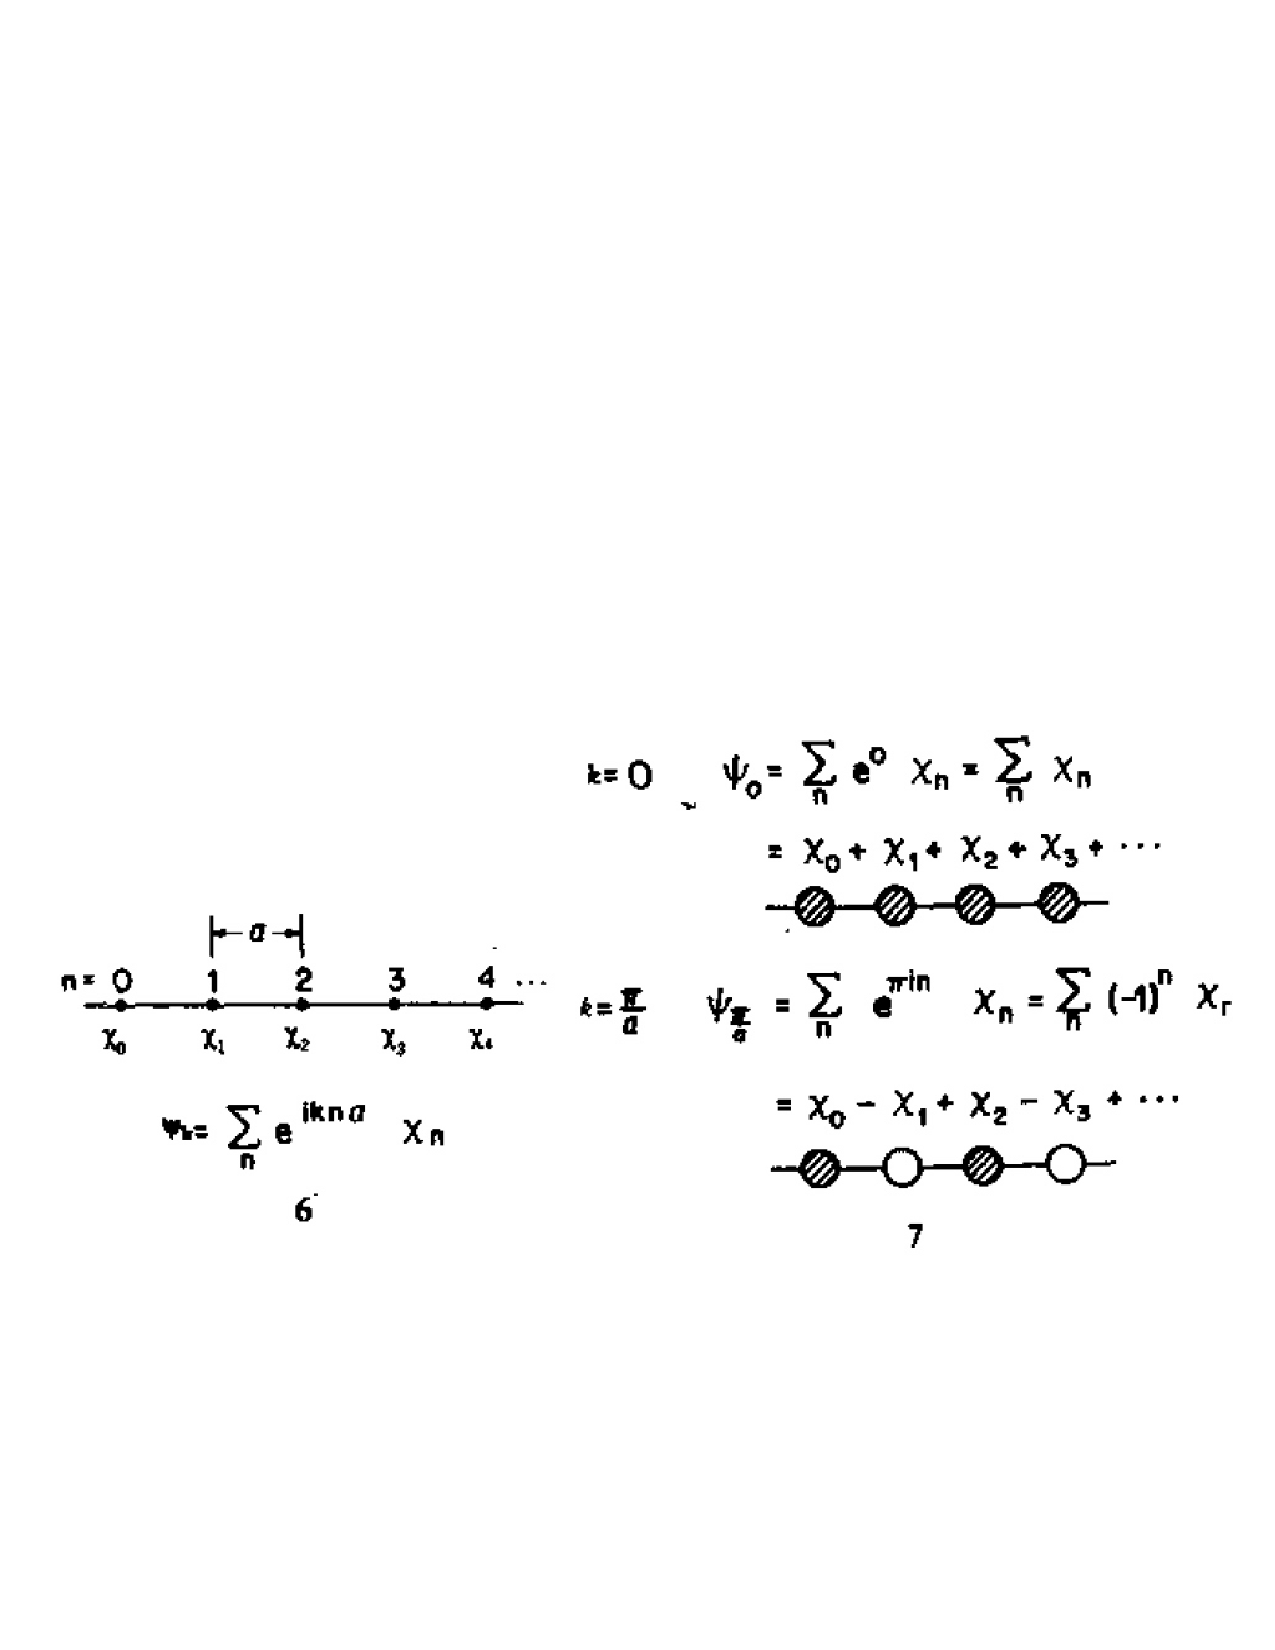
\includegraphics[height=0.5in,width=1.4in,viewport=25 218 595 440,clip]{Figures/Hydrogen-Psi.pdf}}\\
\subfigure[分子轨道与能带]{
\label{fig:Hydrogen-Band-1D}
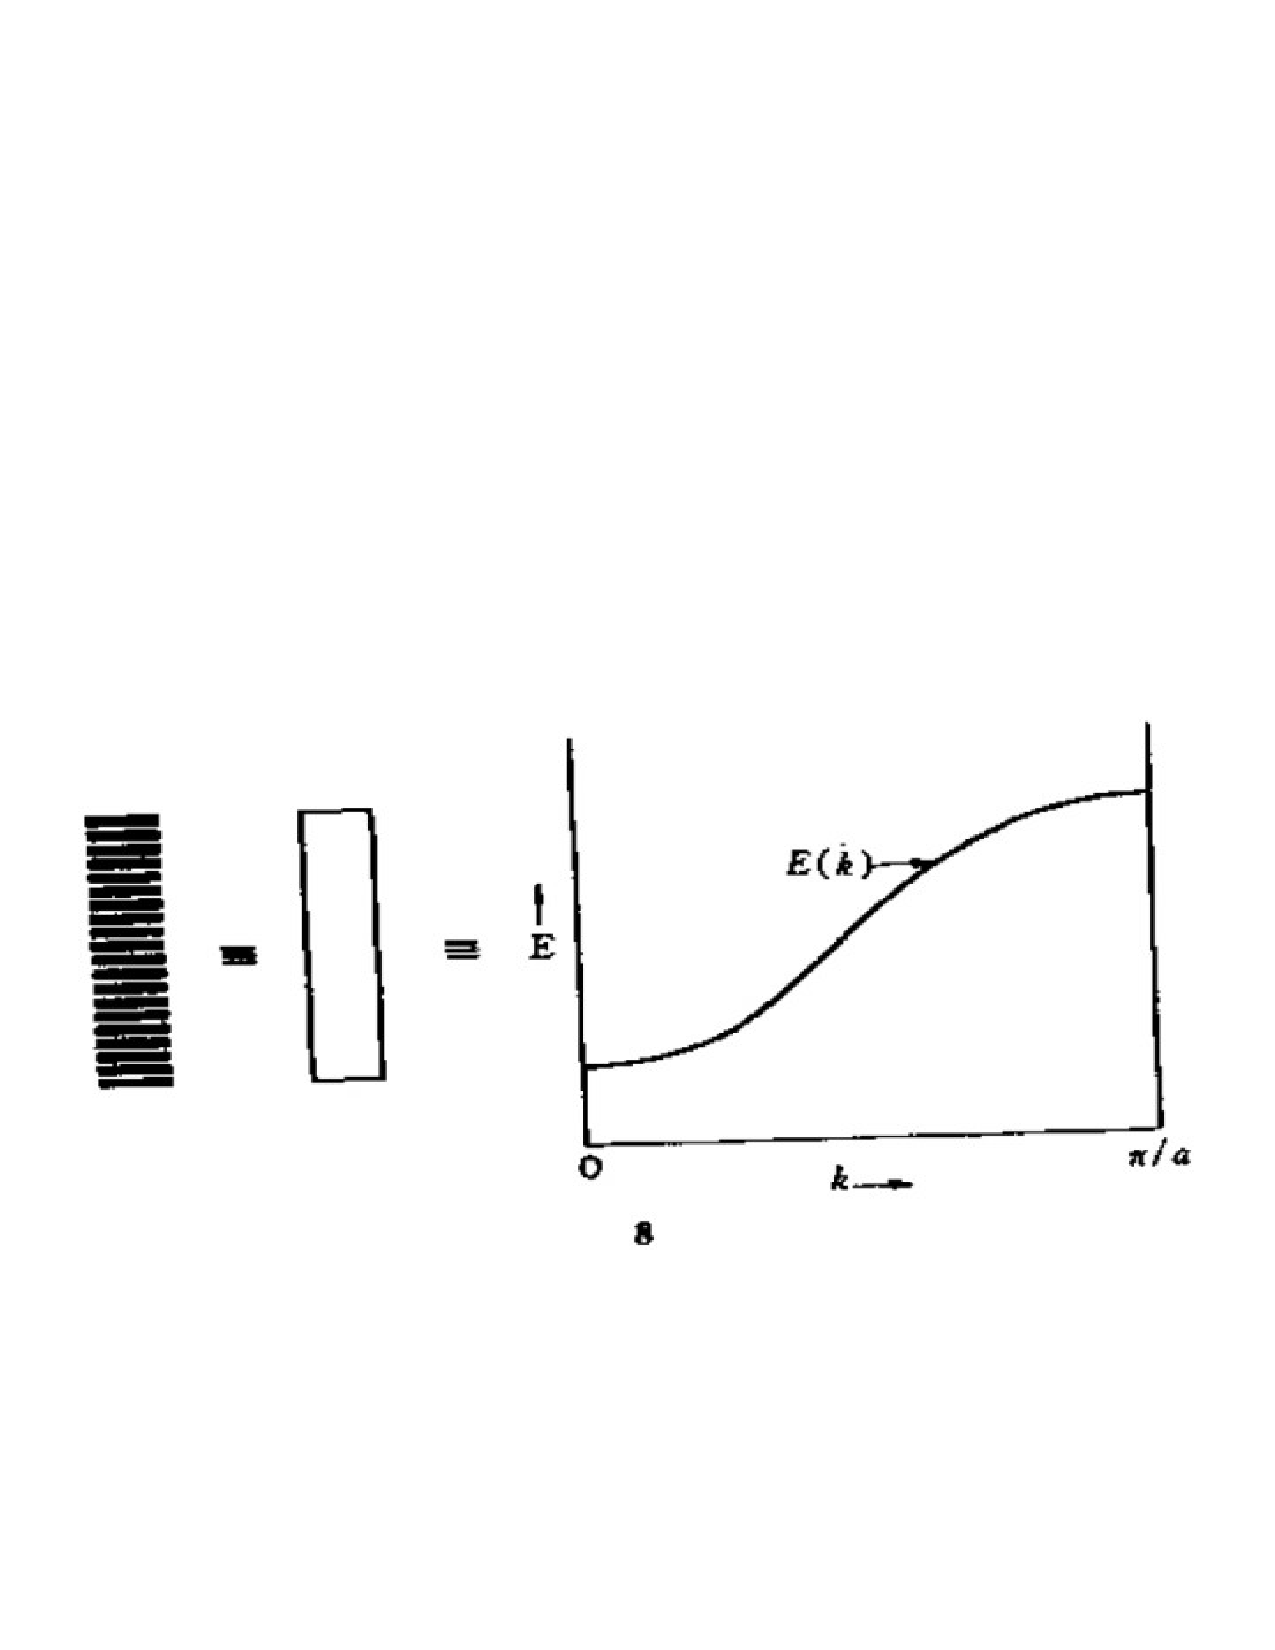
\includegraphics[height=0.6in,width=1.4in,viewport=35 215 575 450,clip]{Figures/Hydrogen-Band-1D.pdf}}
\subfigure[$d$\,轨道]{
\label{fig:Hydrogen-d-Band-1D}
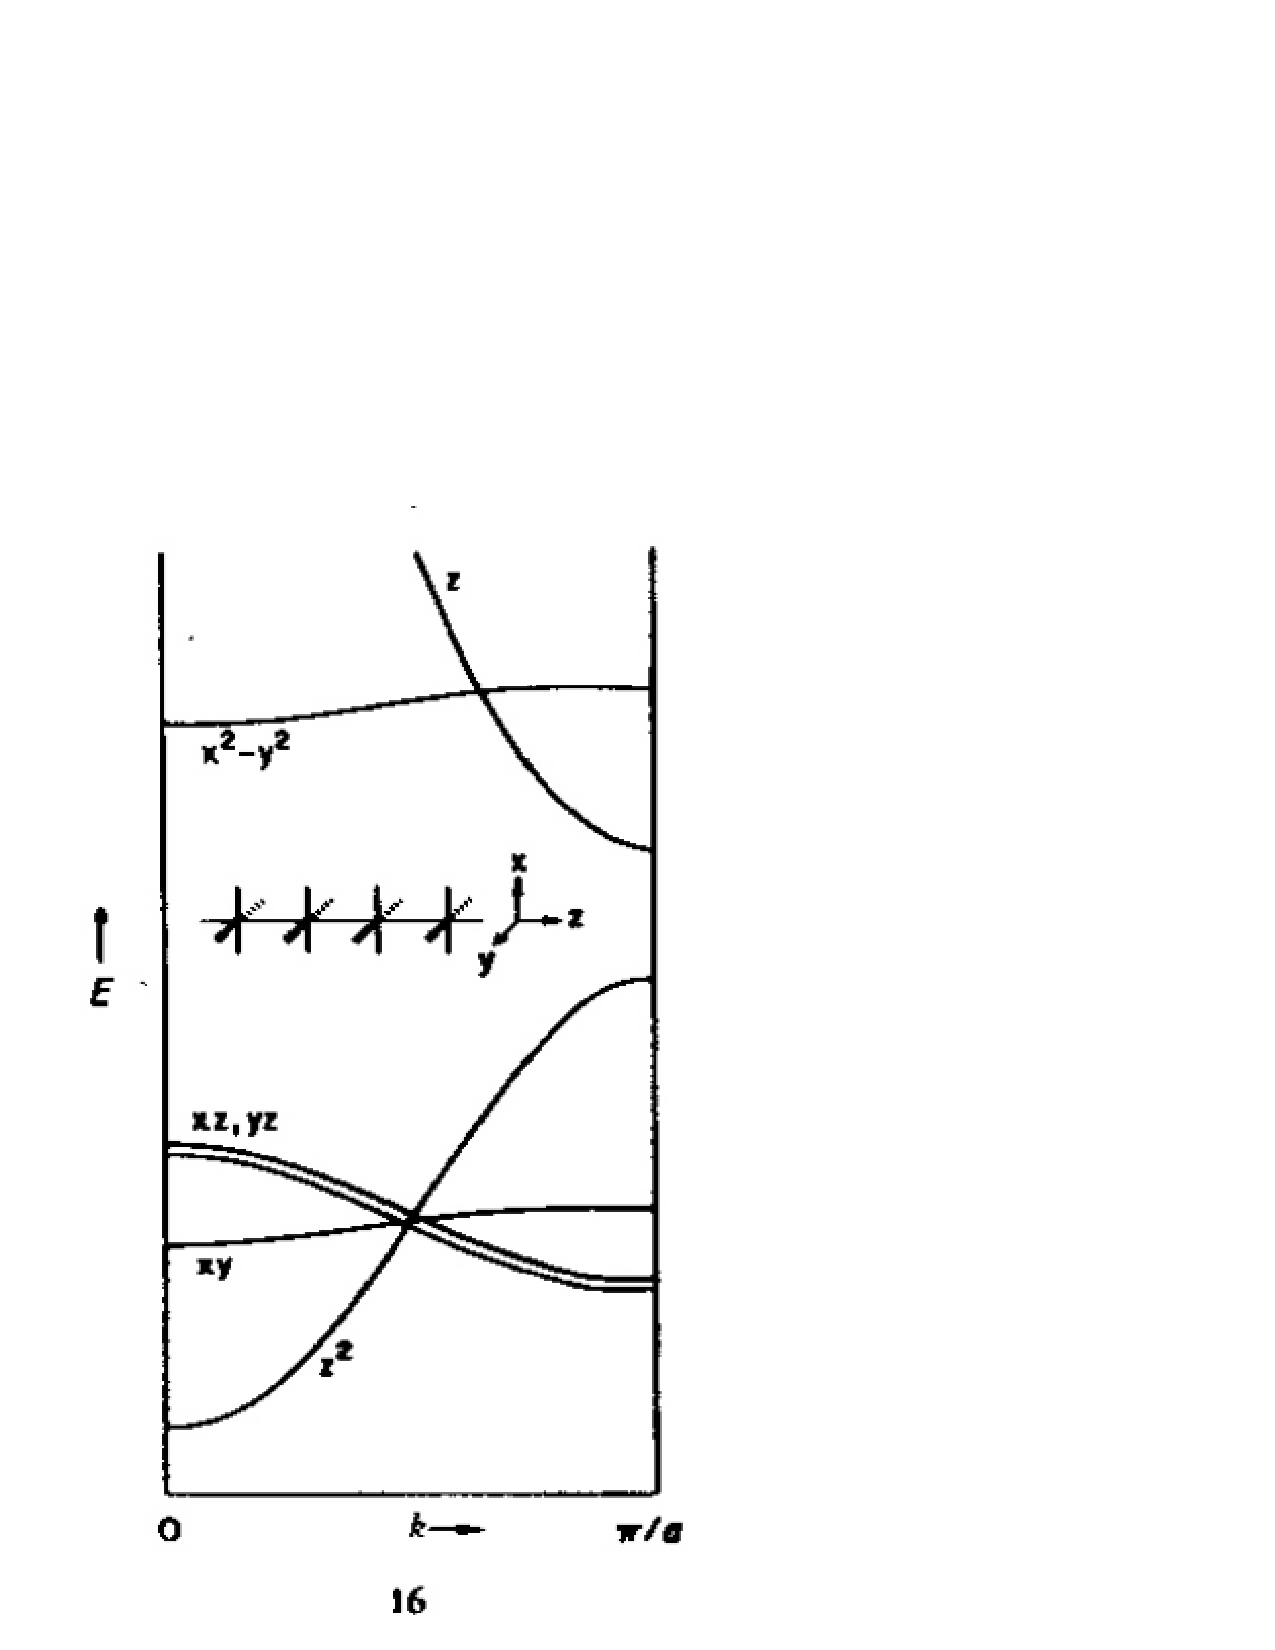
\includegraphics[height=1.0in,width=0.7in,viewport=40 45 330 535,clip]{Figures/Hydrogen-d-Band-1D.pdf}}
\caption{\small \textrm{The Band-structure from Molecular-orbital.}}%
\label{Band-Structure-1}
\end{figure} 
}

\subsection{能带、$\vec k$-空间与~\rm{Fermi~}面}
\frame
{
\frametitle{能带、$\vec k$空间与\textrm{Fermi}面}
\vspace{30pt}
\begin{figure}[h!]
\centering
\hspace*{-0.30in}
\subfigure[\textrm{Band structure}]{
\label{Band_Gap_Fermi-1}
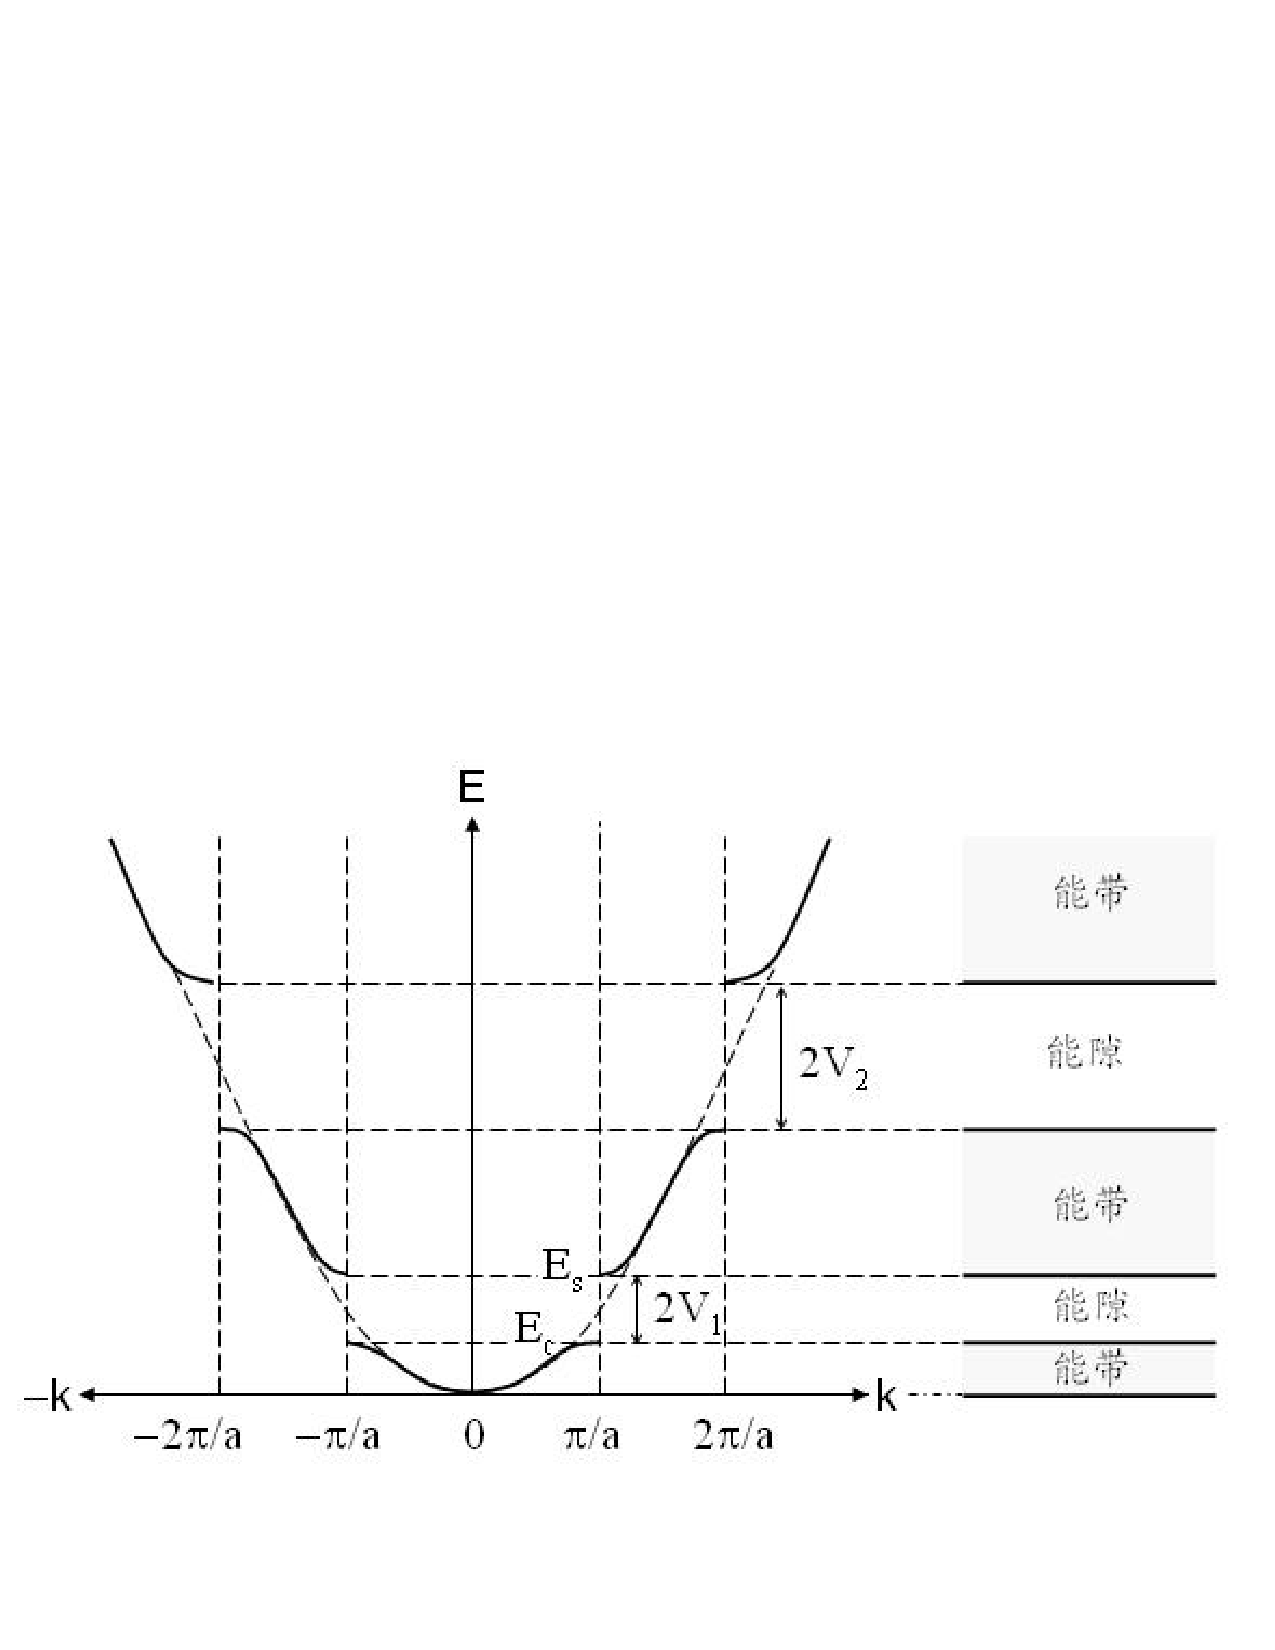
\includegraphics[height=1.3in,width=2.3in,viewport=10 90 570 380,clip]{Figures/Band_Gap.pdf}}
\subfigure[\textrm{Brillouin Zone}]{
\label{Band_Gap_Fermi-2}
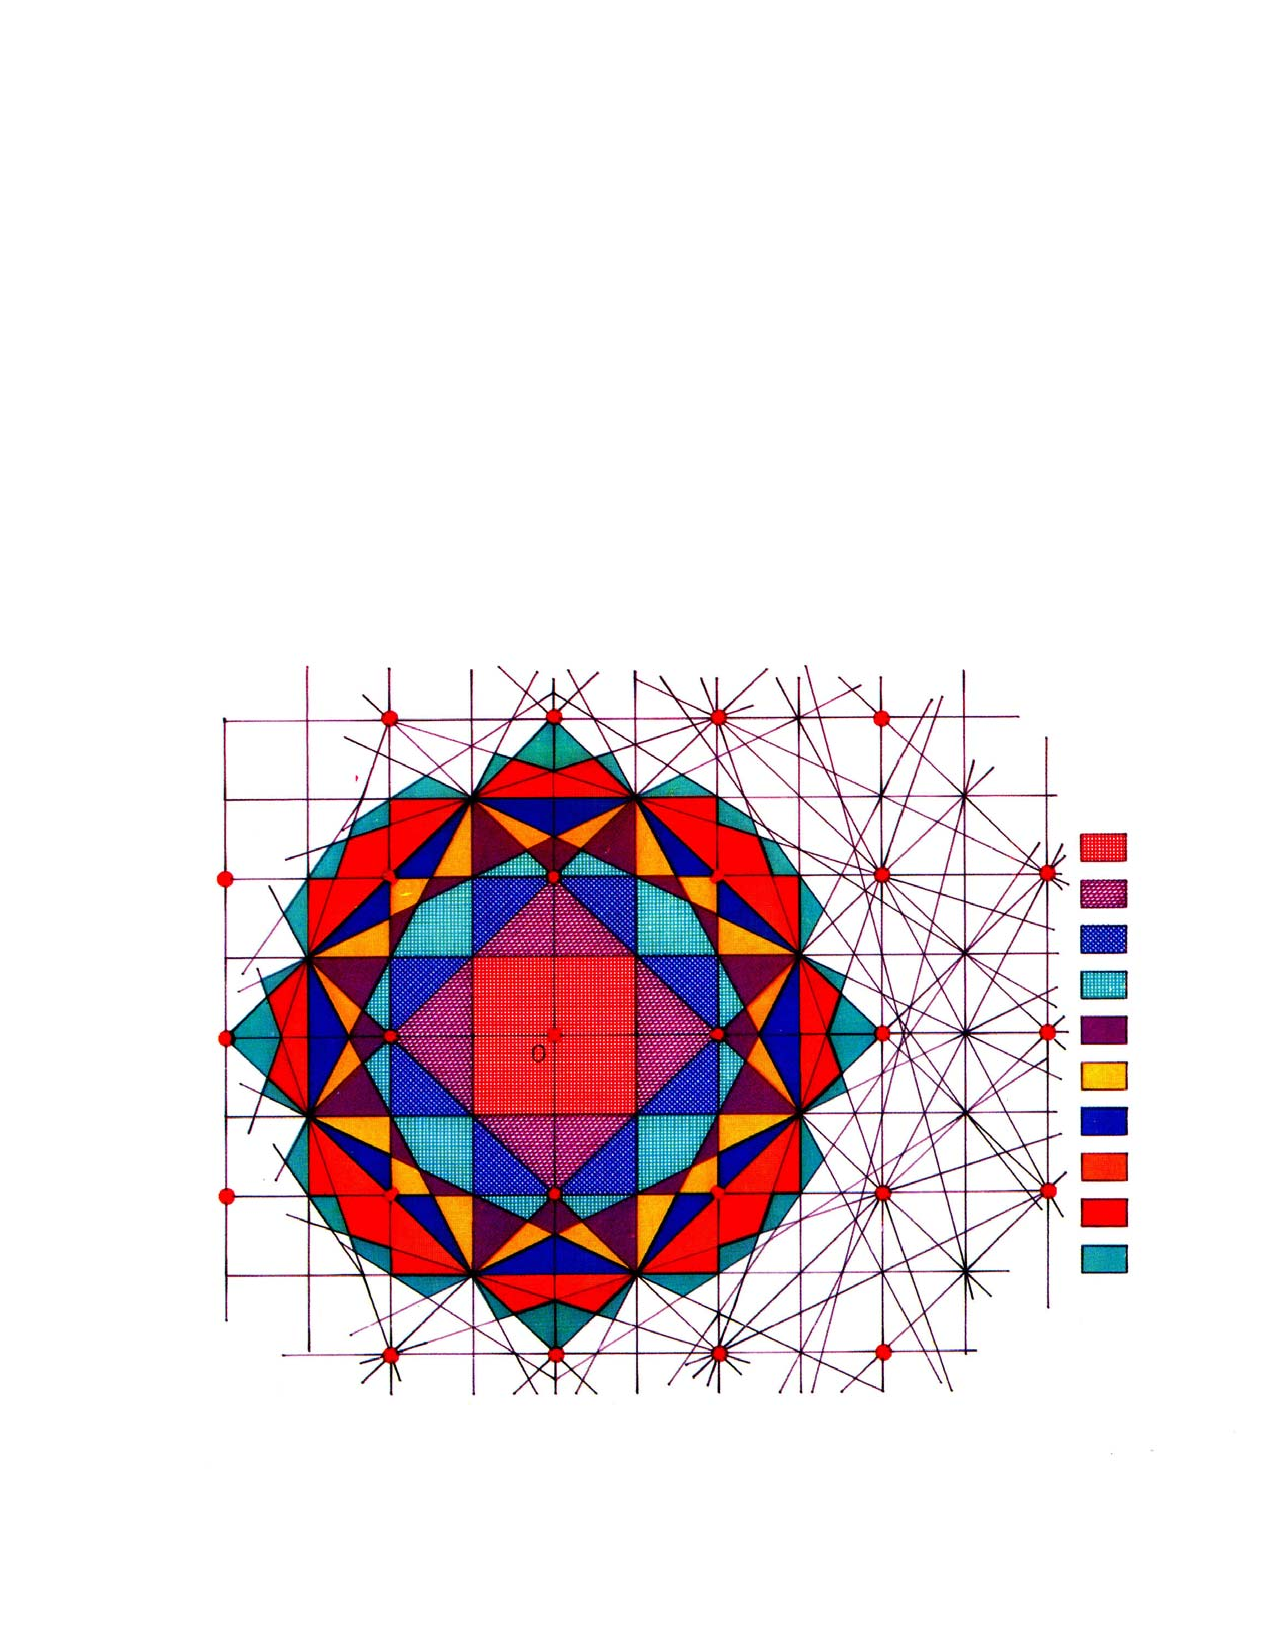
\includegraphics[height=1.28in,width=1.75in,viewport=100 120 545 470,clip]{Figures/2D_Brillouin-Zone.pdf}}
\label{Band_Gap_Fermi}
\end{figure}
}

\frame
{
	\frametitle{简单立方体系的\textrm{Brillouin}区与能带}
\vspace{10pt}
\begin{figure}[h!]
\centering
\hspace*{-0.28in}
\subfigure[\textrm{Brillouin Zone of Cubic lattice}]{
\label{Brillouin_Zone_Cubic}
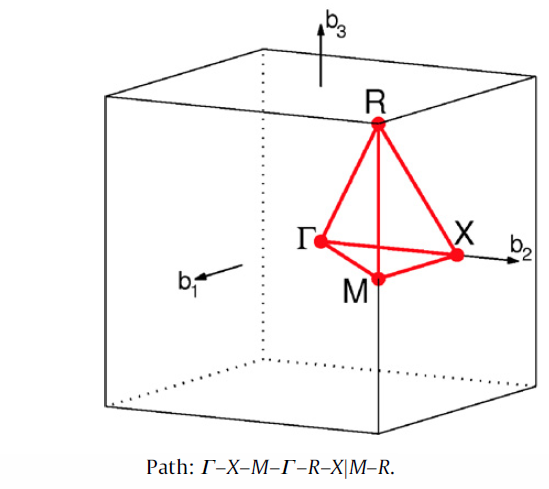
\includegraphics[height=2.1in,width=2.0in,viewport=90 0 550 500,clip]{Figures/Brillouin-Zone_CUB.png}}
\subfigure[\textrm{Band Structure of SrSnO$_3$}]{
\label{Band_Gap_SrSnO3}
\vspace*{-1.00in}
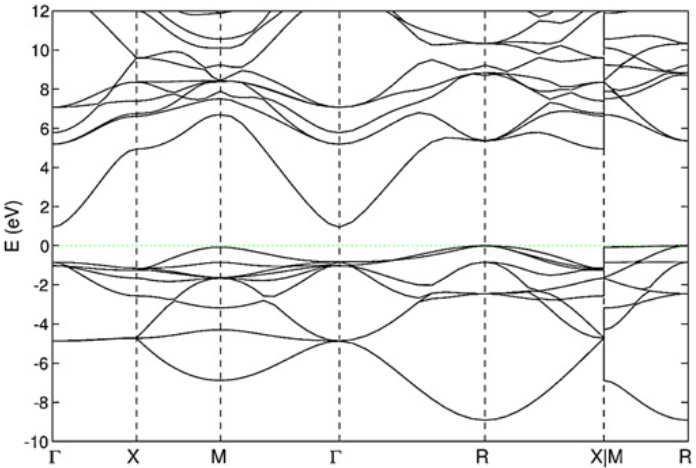
\includegraphics[height=2.10in,width=1.75in,viewport=0 0 710 550,clip]{Figures/Band-Struct_SrSnO3.png}}
\label{Band_Gap_CUB_SrSnO3}
\end{figure}
}

\frame
{
	\frametitle{面心立方体系的\textrm{Brillouin}区与能带}
\vspace{10pt}
\begin{figure}[h!]
\centering
\hspace*{-0.30in}
\subfigure[\textrm{Brillouin Zone of FCC lattice}]{
\label{Brillouin_Zone_FCC}
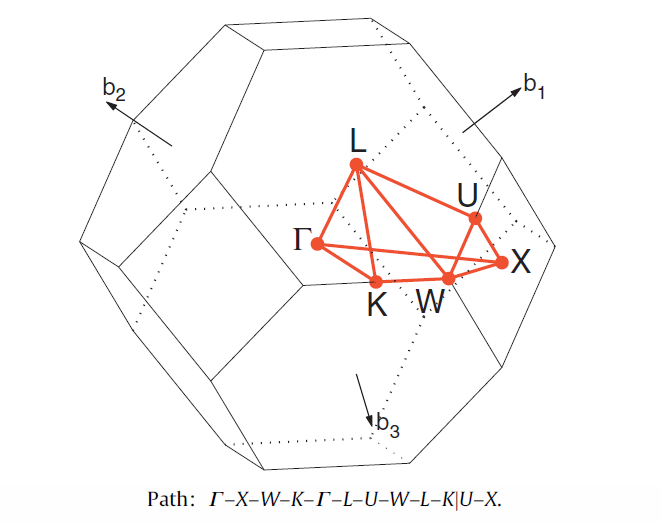
\includegraphics[height=1.9in,width=1.8in,viewport=75 0 560 520,clip]{Figures/Brillouin-Zone_FCC.png}}
\subfigure[\textrm{Band structure of CdS}]{
\label{Band_Gap_CdS}
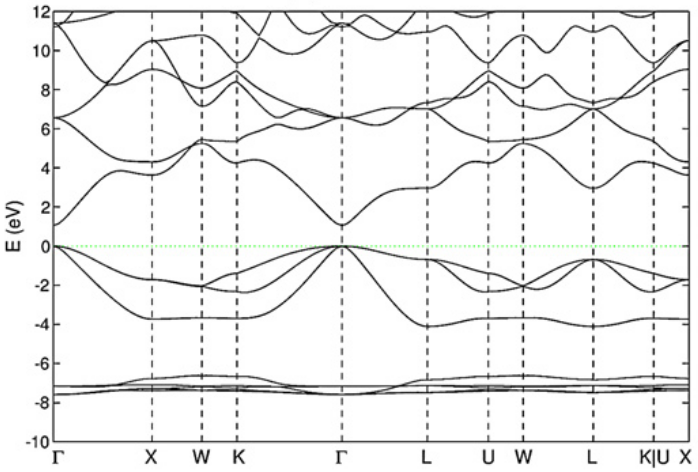
\includegraphics[height=2.10in,width=1.95in,viewport=0 0 700 520,clip]{Figures/Band-Struct_CdS.png}}
\label{Band_Gap_FCC_CdS}
\end{figure}
}

\frame
{
	\frametitle{体心立方体系的\textrm{Brillouin}区与能带}
\vspace{10pt}
\begin{figure}[h!]
\centering
\hspace*{-0.30in}
\subfigure[\textrm{Brillouin Zone of BCC lattice}]{
\label{Brillouin_Zone_BCC}
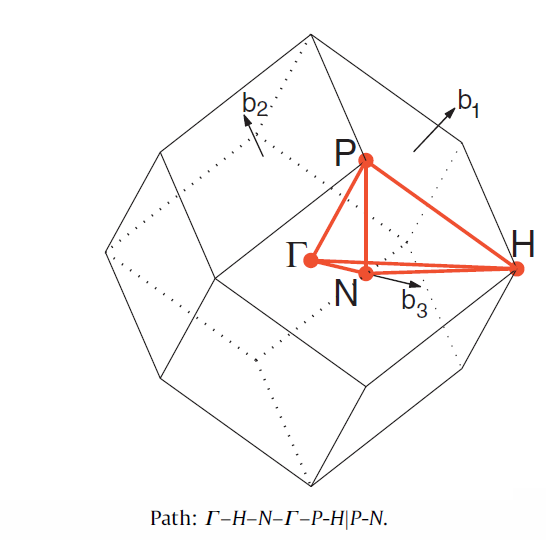
\includegraphics[height=2.1in,width=1.9in,viewport=80 0 550 520,clip]{Figures/Brillouin-Zone_BCC.png}}
\subfigure[\textrm{Band structure of GeF$_4$}]{
\label{Band_Gap_GeF4}
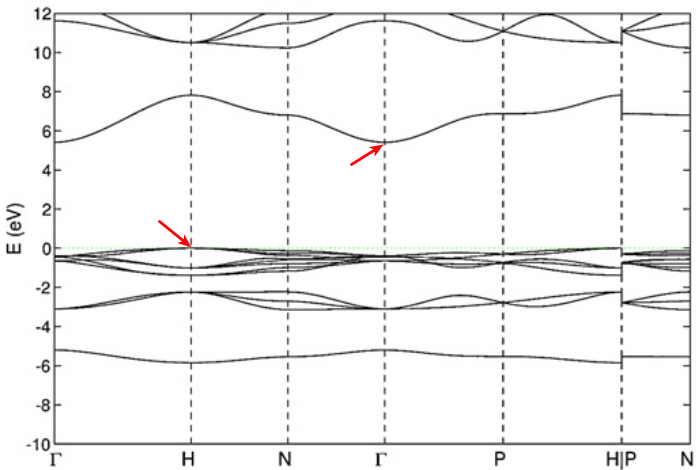
\includegraphics[height=2.10in,width=1.95in,viewport=0 0 700 500,clip]{Figures/Band-Struct_GeF4.png}}
\label{Band_Gap_BCC_GeF4}
\end{figure}
}

\frame
{
%\frametitle{The methods on band structure calculation}
\frametitle{固体能带计算方法}
%\vskip 10pt
%\textrm{The mainly difference of all these methods below: the basis sets and the construction of the potential}
\vskip 10pt
常用的计算方法
\begin{itemize}%[+-| alert@+>]
%\begin{enumerate}%[+-| alert@+>]
\setlength{\itemsep}{12pt}
%  \item \textrm{Plane wave and the pseudo-potential}
	\item	平面波方法
	\item	正交平面波\textrm{(The orthogonalized plane wave, OPW)}和赝势\textrm{(Pseudo-potential, PP)}方法\upcite{Singh_Book,PRB41-7892_1990,JPCM6-8245_1994}
	\item	缀加平面波\textrm{(Augmented plane wave, APW)}方法
	\item	\textrm{MT}轨道\textrm{(Muffin-tin orbitals, MTO)}方法
	\item	投影子缀加波\textrm{(Projector Augmented Wave, PAW)}方法\upcite{PRB50-17953_1994,PRB59-1758_1999}
\end{itemize}
\vskip 5pt 各种方法的\textcolor{red}{主要区别}:~\textcolor{blue}{势函数的处理}与\textcolor{blue}{所选基函数类型}不同
}

\frame
{
	\frametitle{\textrm{DFT-SCF}}
\begin{figure}[h!]
\centering
\vspace*{-0.25in}
\hspace*{-0.80in}
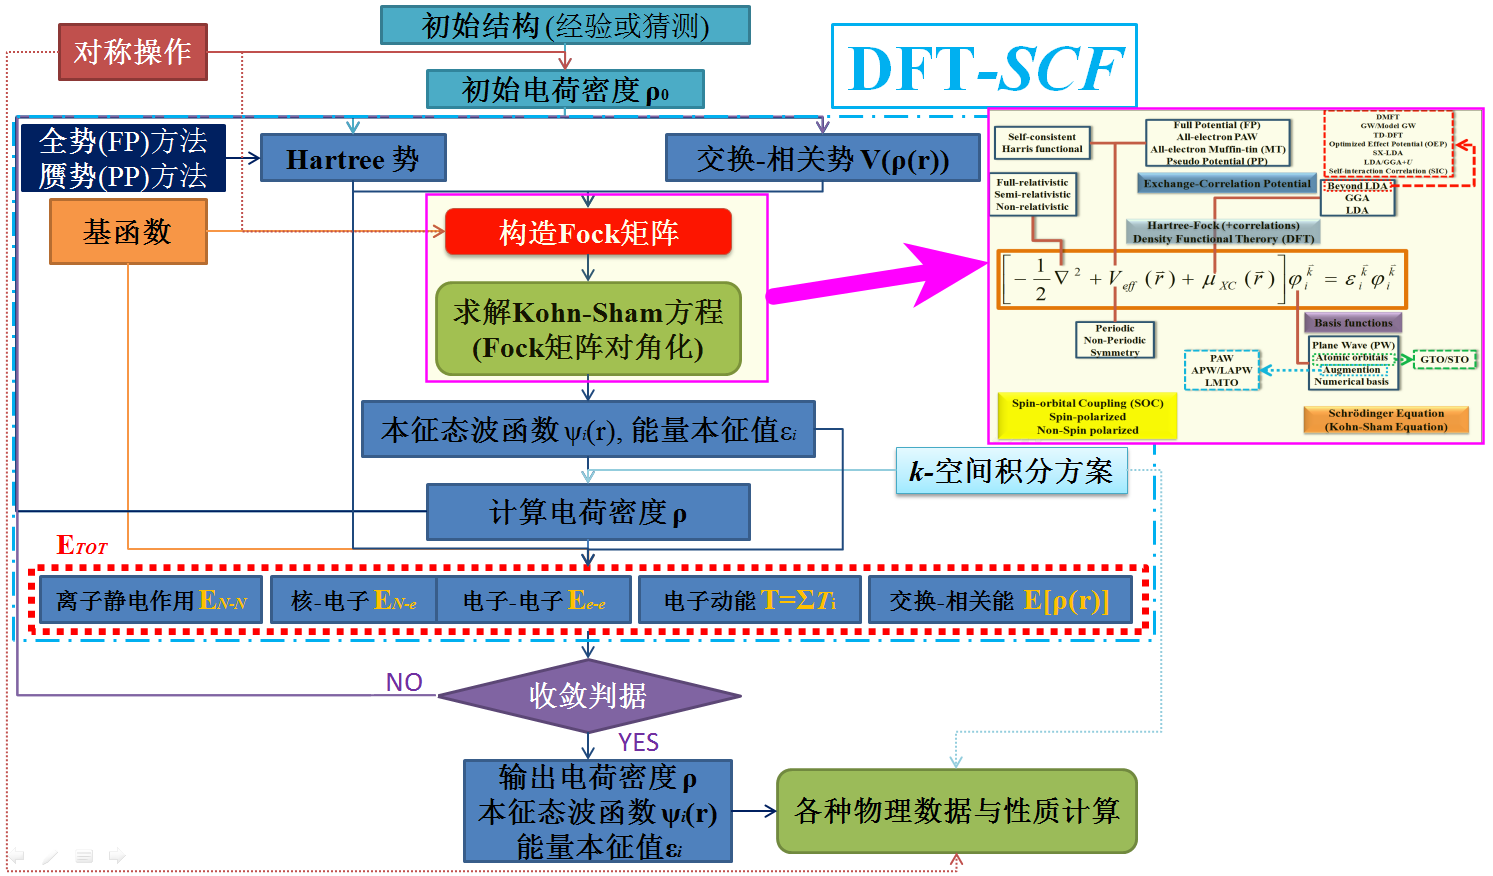
\includegraphics[height=2.80in,width=4.95in,viewport=5 3 1490 870,clip]{Figures/DFT-SCF_2.png}
%\caption{\small \textrm{Pseudopotential for metallic sodium, based on the empty core model and screened by the Thomas-Fermi dielectric function.}}%(与文献\cite{EPJB33-47_2003}图1对比)
\label{Pseudo-NC}
\end{figure}
}

\frame
{
%	\frametitle{\textrm{DFT-SCF}}
\begin{figure}[h!]
\vspace*{-0.25in}
\centering
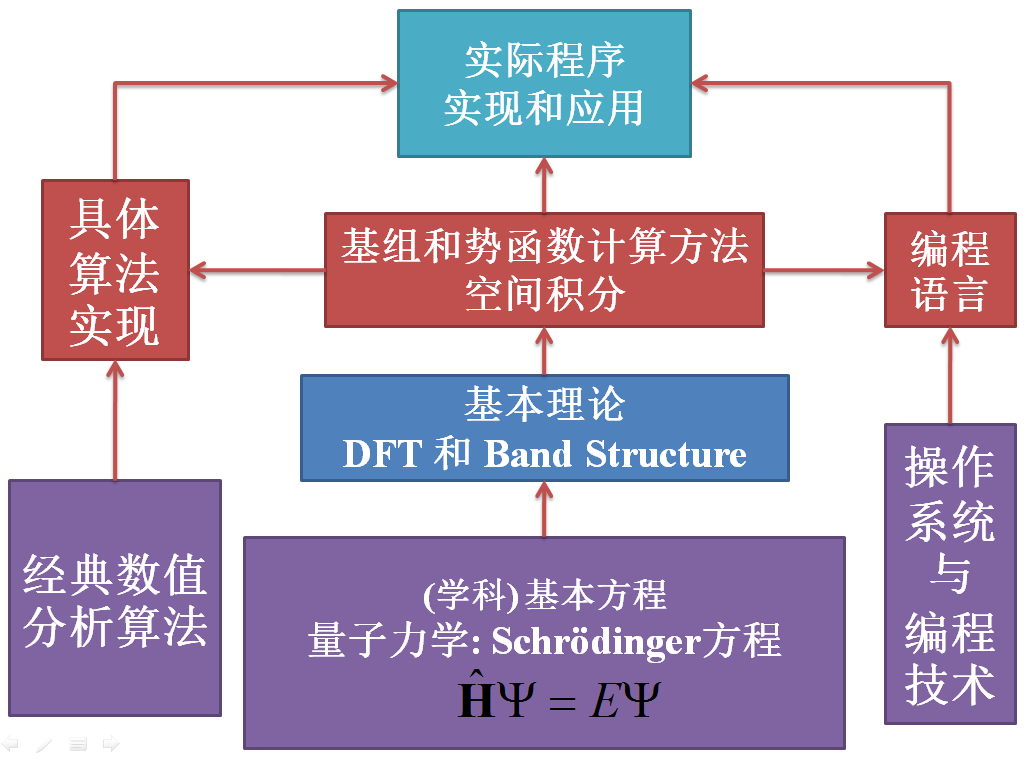
\includegraphics[height=2.80in,width=4.95in,viewport=5 3 1250 780,clip]{Figures/Method_Procedure.png}
%\caption{\small \textrm{Pseudopotential for metallic sodium, based on the empty core model and screened by the Thomas-Fermi dielectric function.}}%(与文献\cite{EPJB33-47_2003}图1对比)
\label{Method-Procedure}
\end{figure}
}

\section{赝势理论}       %Bookmark
%\section{Induction on DFT and solid-state physics}       %Bookmark
\subsection{平面波与赝势}       %Bookmark
\frame
{
	\frametitle{球形势对平面波的散射与相移}
\begin{figure}[h!]
\centering
\vspace*{-0.26in}
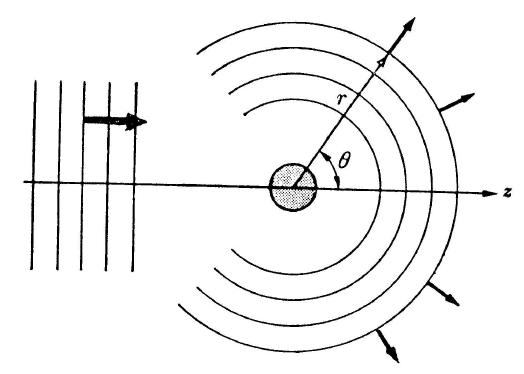
\includegraphics[height=0.90in,width=1.24in,viewport=0 0 400 300,clip]{Figures/Pseudo-scatter.jpg}
\caption{\small \textrm{Schematic illustration of scattering of a plane wave by a spherical potential.}}%(与文献\cite{EPJB33-47_2003}图1对比)
\label{Pseudo-scatter}
\end{figure}
$$\mathrm{e}^{\mathrm{i}\vec q\cdot\vec r}=4\pi\sum_{lm}\mathrm{i}^lj_l(\vec q\cdot\vec r)Y_{lm}^{\ast}(\hat{\vec q})Y_{lm}(\hat{\vec r})=\sum_{l}(2l+1)\mathrm{i}^lj_l(qr)P_{l}(\cos\theta)$$
%$$\mathrm{e}^{\mathrm{i}\vec q\cdot\vec r}=\mathrm{e}^{\mathrm{i}qr\cos(\theta)}=\sum_{l}(2l+1)\mathrm{i}^lj_l(qr)P_{l}[\cos(\theta)]$$
$$\Psi_l^{>}(\varepsilon,r)=C_l\bigg[j_l(\kappa r)-\tan\eta_l(\varepsilon)n_l(\kappa r)\bigg]\quad\text{其中}\kappa^2=\varepsilon$$
$$D_l(\varepsilon,r)\equiv r\psi_l^{\prime}(r)/\psi_l(r)=r\dfrac{\mathrm{d}}{\mathrm{d}r}\ln\psi_l(r)$$
$$\tan\eta_l(\varepsilon)=\dfrac{R\frac{\mathrm{d}}{\mathrm{d}r}j_l(\kappa r)|_R-D_l(\varepsilon)j_l(\kappa R)}{R\frac{\mathrm{d}}{\mathrm{d}r}n_l(\kappa r)|_R-D_l(\varepsilon)n_l(\kappa R)}$$
%$$t(\theta)=\dfrac{4\pi}{\sqrt\varepsilon}\sum_l(2l+1)\bigg[\mathrm{e}^{2\mathrm{i}\eta_l}-1\bigg]P_l(\cos\theta)$$
%$$\eta_l(\varepsilon)=p_l\pi+\delta_l(\varepsilon)$$
}

\frame
{
	\frametitle{散射相移与赝势}
\begin{figure}[h!]
\centering
\vspace*{-0.25in}
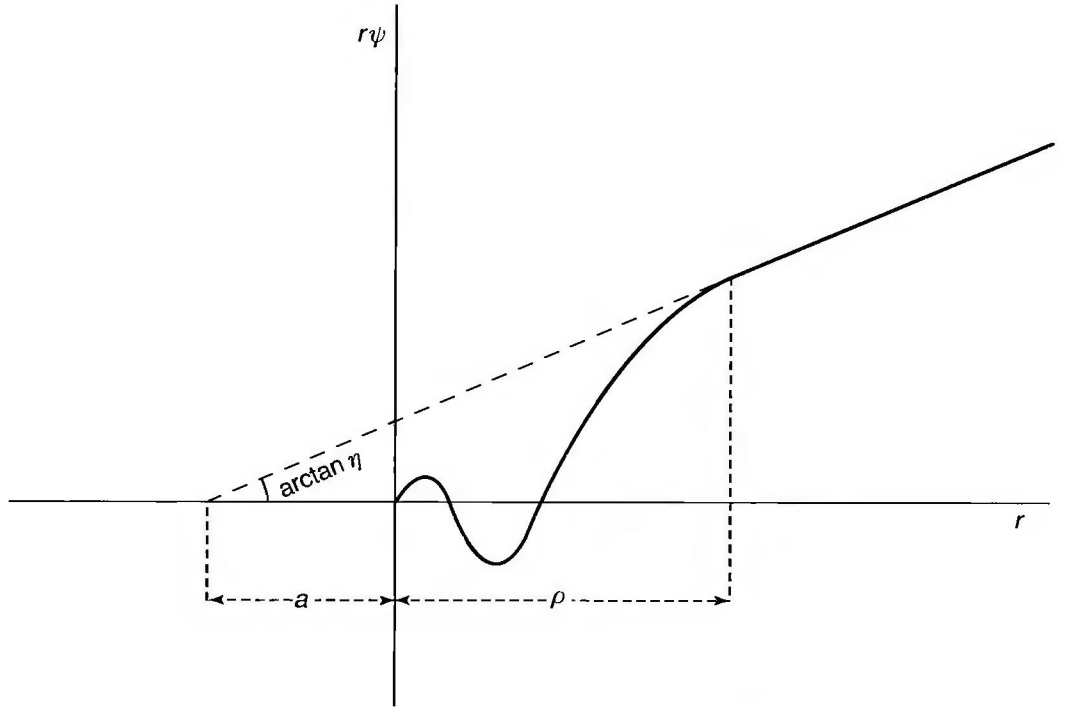
\includegraphics[height=1.50in,width=2.27in,viewport=0 0 1150 750,clip]{Figures/Pseudo-scatter-2.png}
\caption{\fontsize{9.5pt}{8.2pt}\selectfont{\textrm{Radial wave-function $\phi=r\psi$ for low-energy scattering as illustrated in a figure from the 1934 and 1935 papers of Fermi and coworkers for low-energy electron scattering from atoms and neutron scattering from nuclei. The node in the wave-function near the origin show that the potential is attractive and strong enough to have bound states. The cross-section for scattering from the localized potential is determined by the phase shift and is the same for weaker pseudo-potential with the same phase shift modulo $2\pi$.}}}%(与文献\cite{EPJB33-47_2003}图1对比)
\label{Pseudo-scatter-2}
\end{figure}
}

\frame
{
%\frametitle{The methods on band structure calculation}
	\frametitle{由\textrm{OPW~}到赝势}
%\vskip 10pt
%\textrm{The mainly difference of all these methods below: the basis sets and the construction of the potential}
\begin{itemize}
\setlength{\itemsep}{5pt}
	\item 完全平面波基组:~少数平面波就可以很好地描述波函数在原子间的行为,近核波函数则需要大量平面波展开。%因此完全平面波基组虽然方便,但求体系本征态对角化的矩阵非常巨大,计算变得异常耗时。
	\item 正交平面波(\textrm{Orthogonalized plane wave, OPW})方法,价电子用与芯层波函数正交的平面波展开
		\begin{displaymath}
			\phi_{OPW}^{\vec k+\vec G}(\vec r)=\phi_{PW}^{\vec k+\vec G}(\vec r)-\sum_c\langle\varphi_c|\phi_{PW}^{\vec k+\vec G}\rangle\varphi_c(\vec r)
		\end{displaymath}
		代入\textrm{Schr\"odinger}方程
		$$\hat H|\phi_{PW}^{\vec k+\vec G}\rangle-\sum_c\langle\varphi_c|\phi_{PW}^{\vec k+\vec G}\rangle\hat H|\varphi_c\rangle=\varepsilon|\phi_{PW}^{\vec k+\vec G}\rangle-\varepsilon\sum_c\langle\varphi_c|\phi_{PW}^{\vec k+\vec G}\rangle|\varphi_c\rangle$$
		可有$$\hat H|\phi_{PW}^{\vec k+\vec G}\rangle+\textcolor{blue}{V^R}|\phi_{PW}^{\vec k+\vec G}\rangle=\textcolor{blue}{\varepsilon}|\phi_{PW}^{\vec k+\vec G}\rangle$$
%		这里排斥势是$$V^R(\vec r,\vec r^{\prime})=\sum_c(\varepsilon-\varepsilon_c)|\varphi_c(\vec r^{\prime})\rangle\langle\varphi_c(\vec r)|$$
\end{itemize}
}

\frame
{
	\frametitle{由\textrm{OPW~}到赝势}
	\textrm{Phillips-Kleinman}指出赝势($V^{eff}$)-赝波函数(可用$\phi_{PW}^{\vec k+\vec G}$展开)满足\textrm{Schr\"odinger}方程\upcite{PR116_1959}
	$$\bigg(-\dfrac12\nabla^2+\textcolor{red}{V^{eff}}\bigg)|\phi_{PW}^{\vec k+\vec G}\rangle=\textcolor{blue}{\varepsilon}|\phi_{PW}^{\vec k+\vec G}\rangle$$
	其中$\textcolor{red}{V^{eff}}=V(\vec r)+\textcolor{blue}{V^R}$
	\begin{itemize}
		\item 赝势-赝波函数的本征值$\varepsilon$与真实体系的能量本征值等价
		\item 赝势$V^{eff}$比$V(\vec r)$平滑得多,并且$V^R$是非局域的排斥势
			\begin{displaymath}
				\begin{aligned}
					V^Rf(\vec r)=&\sum_c(\varepsilon-\varepsilon_c)\varphi_c(\vec r)\int\varphi_c^{\ast}(\vec r^{\prime})f(\vec r^{\prime})\mathrm{d}\vec r^{\prime} \\
					=&\int V^R(\vec r,\vec r^{\prime})f(\vec r^{\prime})\mathrm{d}\vec r^{\prime}
				\end{aligned}
			\end{displaymath}
			这里$$V^R(\vec r,\vec r^{\prime})=\sum_c(\varepsilon-\varepsilon_c)|\varphi_c(\vec r^{\prime})\rangle\langle\varphi_c(\vec r)|$$
	\end{itemize}
}

\frame
{
\frametitle{赝势方法}
赝势(\textrm{Pseudo Potential, PP})方法是在正交平面波的基础上发展起来的,构造出平缓的势函数代替核的强吸引作用和芯层电子的排斥作用,用平缓的函数取代波函数近核时的震荡。
\begin{itemize}
\setlength{\itemsep}{5pt}
	\item 赝势-平面波方法,只需要少量平面波可展开赝波函数,大大提升了计算效率;但是赝波函数不能很好地反映与电子近核行为有关的性质。
	\item 赝势的构造并不唯一,考核构造赝势的两大指标:~\\“柔软程度”\textrm{(Soft)}与“可移植性”\textrm{(transferability)}
\end{itemize}
\begin{figure}[h!]
\centering
\vspace*{-0.10in}
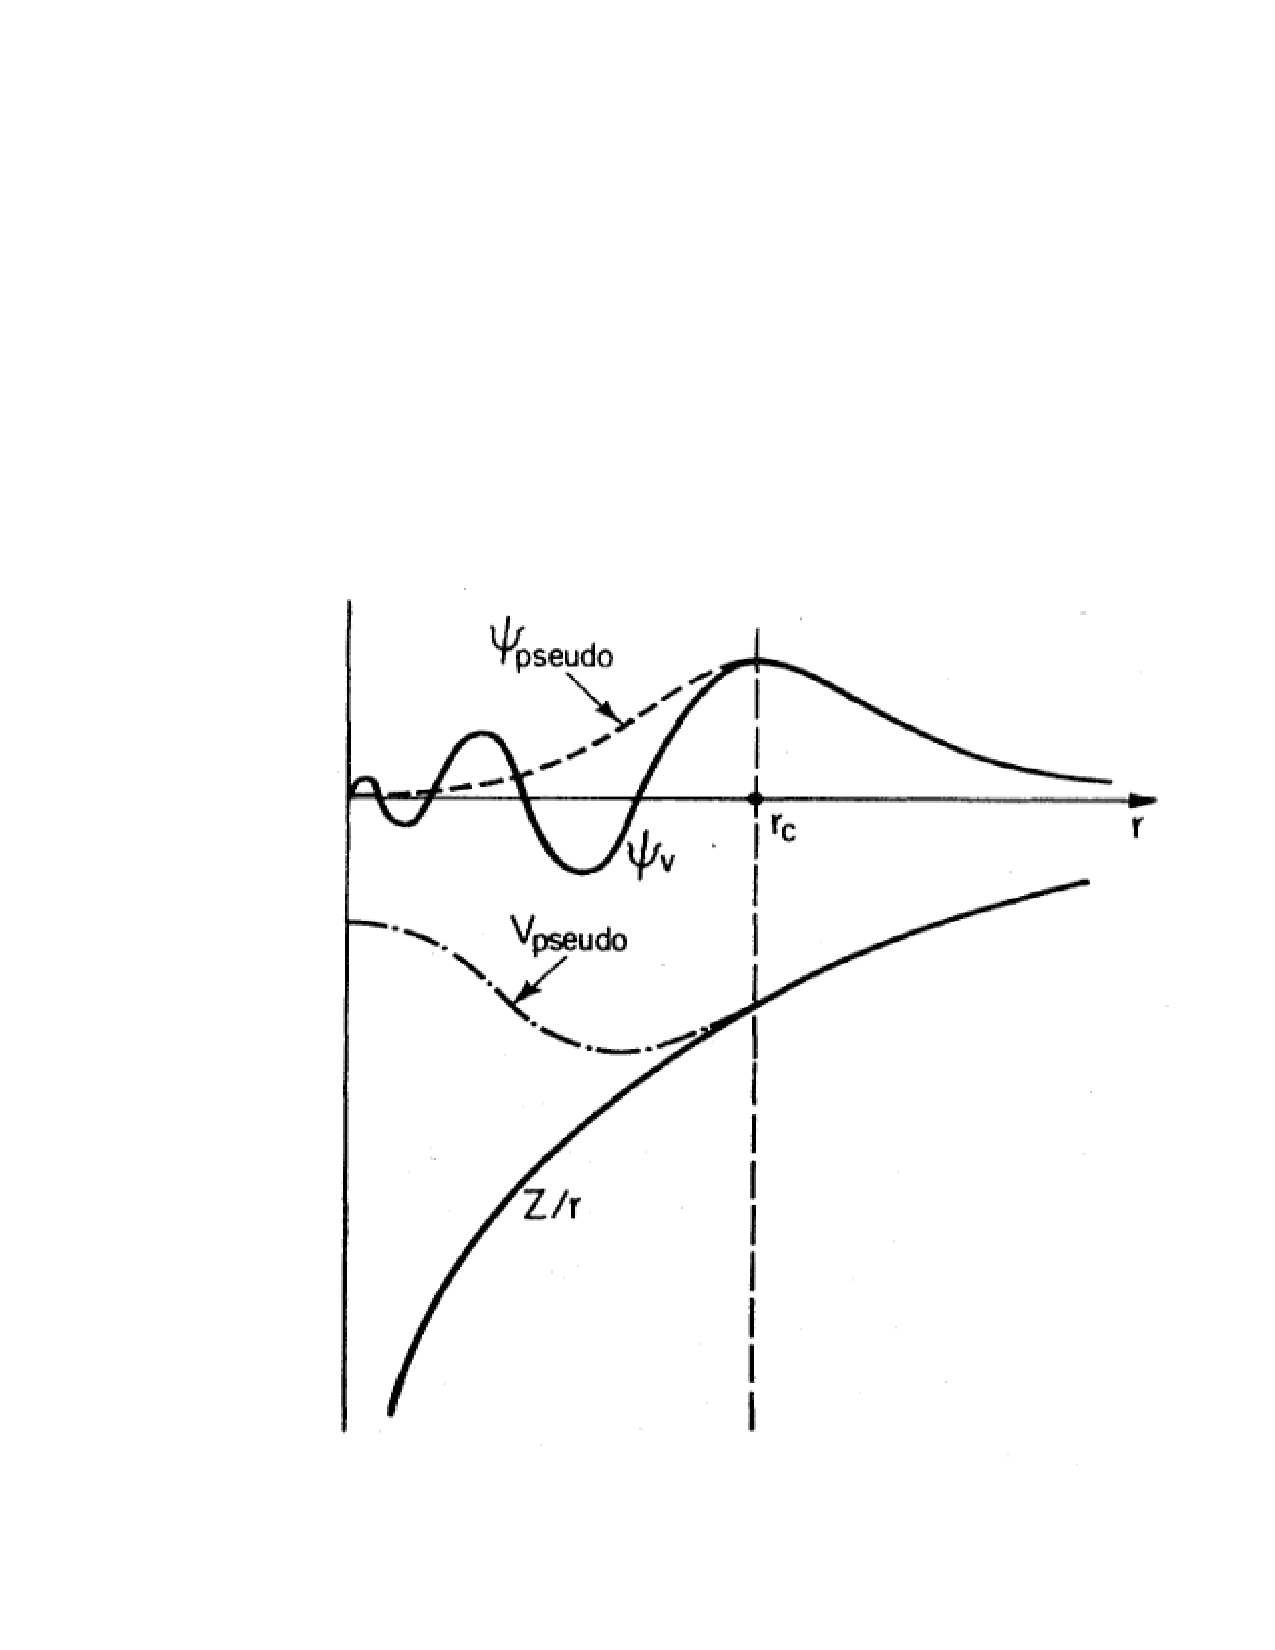
\includegraphics[height=1.35in,width=1.42in,viewport=154 100 562 508,clip]{Figures/Pseudo.pdf}
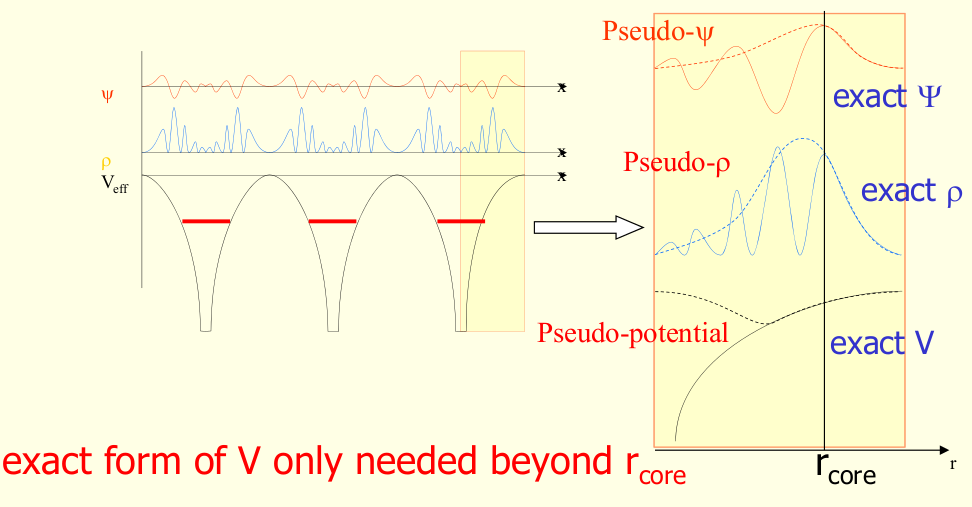
\includegraphics[height=1.35in,width=2.57in,viewport=1 1 980 500,clip]{Figures/Pseudo-2.png}
\caption{\small \textrm{The Pseudo wave function and Pseudo potential.}}%(与文献\cite{EPJB33-47_2003}图1对比)
\label{Pseudo_Potential-Wave}
\end{figure}
}

\subsection{模守恒赝势与超软赝势}
\frame
{
	\frametitle{传统赝势的构造}
	直接由实验数据来确定(模型)赝势,常用的实验数据包括离子对电子的散射角度、离子的光谱实验数据等
		\begin{itemize}
			\item 构造离子赝势:~可移植性好
			\item 构造总赝势(包括全部价电子相互作用):~常用于能带描述
		\end{itemize}
%	\begin{itemize}
%		\item 在指定能量范围内,离子对电子散射的散射角
%		\item 离子的光谱实验数据
%	\end{itemize}
\begin{figure}[h!]
\centering
\vspace*{-0.10in}
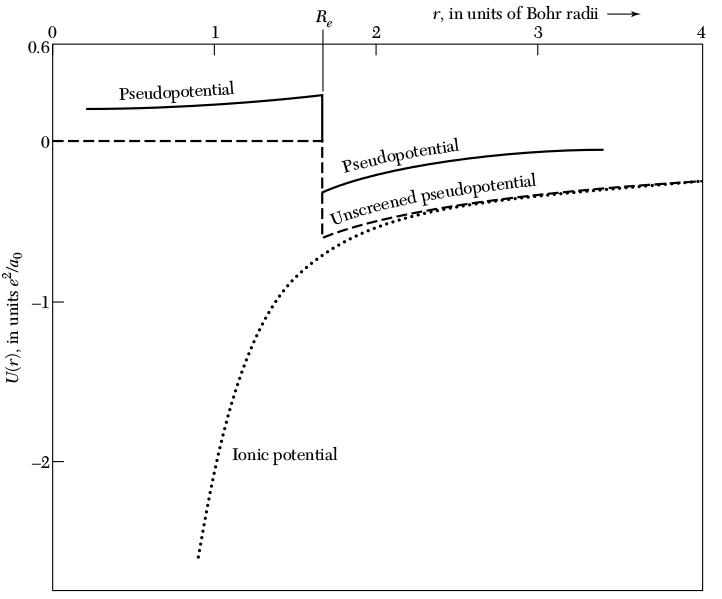
\includegraphics[height=1.60in,width=2.57in,viewport=0 0 980 600,clip]{Figures/Pseudo-model-empty_core.png}
\caption{\small \textrm{Pseudopotential for metallic sodium, based on the empty core model and screened by the Thomas-Fermi dielectric function.}}%(与文献\cite{EPJB33-47_2003}图1对比)
\label{Pseudo_model-empty_core}
\end{figure}
}

\frame
{
	\frametitle{传统赝势的构造}
\begin{figure}[h!]
\centering
\vspace*{-0.10in}
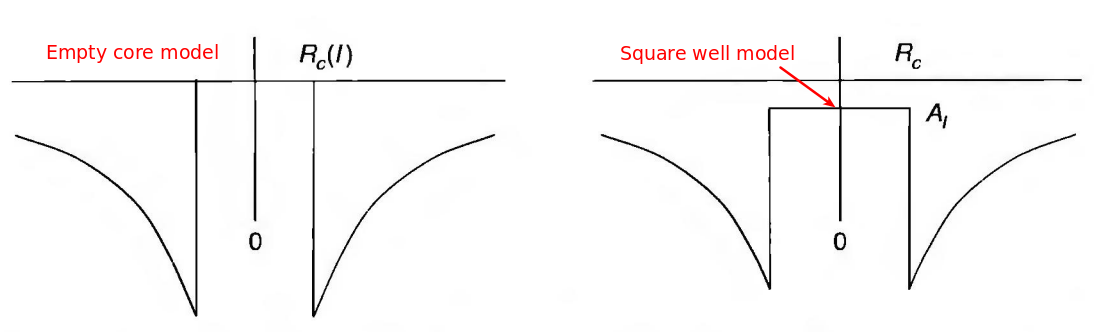
\includegraphics[height=1.30in,width=4.17in,viewport=0 0 1150 350,clip]{Figures/Pseudo-model.png}
\caption{\small \textrm{Left:``Empty core'' model potential of Ashcroft in which the potential is zero inside radius $R_c(l)$ which is different for each $l$. Right: Square well model potential with value $A_l$ inside a cut-off radius $R_c$, proposed by Abarenkov and Heine and fit to atomic data by Animalu and Heine. THe fact that the potential are weak, zero, or even positive inside cut-off radius $R_c$ is an illustration of the ``cancellation theorem''.}}%(与文献\cite{EPJB33-47_2003}图1对比)
\label{Pseudo-model}
\end{figure}
}

\frame
{
	\frametitle{第一原理赝势}
		由第一原理求解出全电子波函数(径向部分)$P_{n,l}(r)$
			\begin{displaymath}
				\bigg[-\dfrac12\dfrac{\mathrm{d}^2}{\mathrm{d}r^2}+\dfrac{l(l+1)}{2r^2}+V(\rho,r)\bigg]P_{n,l}(r)=\varepsilon_{n,l}P_{n,l}(r)
			\end{displaymath}
			这里$V(\rho,r)$是自洽单电子势
			$$V(\rho,r)=-\frac{Z}r+V_{\mathrm H}(\rho,r)+V_{XC}^{\mathrm{LDA}}(\rho(r))$$
			$V_{\mathrm H}(\rho,r)$是\textrm{Hartree}势,$V_{XC}^{\mathrm{LDA}}(\rho(r))$是交换-相关势

			由此构造赝波函数$P_l^{\mathrm{PP}}(r)$,满足
			$$P_l^{\mathrm{PP}}(r)=P_l^{\mathrm{AE}}(r),\quad r>r_{cl}$$
			进而构造赝势$V_{\mathrm{src},l}^{\mathrm{PP}}(r)$
			$$V_{\mathrm{src},l}^{\mathrm{PP}}(r)=\varepsilon_l-\dfrac{l(l+2)}{2r^2}+\dfrac{1}{2P_l^{\mathrm{PP}}(r)}\dfrac{\mathrm{d}^2}{\mathrm{d}r^2}P_l^{\mathrm{AE}}(r),\quad r>r_{cl}$$
}

\frame
{
	\frametitle{模守恒\textrm{(Norm-conserving)}条件}
%	构造赝势确定参数的边界(构造条件)
	\begin{enumerate}
		\item 价电子赝波函数的能量本征值与对应全电子波函数能量本征值相等:~$\varepsilon_l^{\mathrm{PP}}=\varepsilon_l^{\mathrm{AE}}$
		\item 价电子赝波函数与真实电子波函数的径向部分在截断半径$r_{c,l}$外相同:~$\psi_l^{\mathrm{PP}}(r)=\psi_l^{\mathrm{AE}}(r),\quad r>r_{cl}$
		\item 价电子赝波函数与真实电子波函数的对数导数在截断半径$r_{c,l}$处相等:~$D_l^{\mathrm{PP}}(r)=D_l^{\mathrm{AE}}(r),\quad r\geqslant r_{cl}$\\
		这里$D_l(\varepsilon,r)=r\frac{\psi_l^{\prime}(\varepsilon,r)}{\psi_l(\varepsilon,r)}=r\dfrac{\mathrm{d}}{\mathrm{d}r}\ln\psi_l(\varepsilon,r)$
		\item 价电子赝波函数与真实电子波函数在截断半径$r_{c,l}$内的积分电荷相等(\textcolor{red}{模守恒条件})
			$$Q_l=\int_0^{r_{cl}}\mathrm{d}rr^2|\psi_l^{\mathrm{PP}}(r)|^2=\int_0^{r_{cl}}\mathrm{d}rr^2|\psi_l^{\mathrm{AE}}(r)|^2$$
		\item 价电子赝波函数与真实电子波函数的对数导数一阶能量导数$\mathrm{d}D_l(\varepsilon,r)/\mathrm{d}\varepsilon$在截断半径$r_{c,l}$处及以外相等
	\end{enumerate}
}

\frame
{
	\frametitle{模守恒\textrm{(Norm-conserving)}条件}
\begin{figure}[h!]
\centering
\vspace*{-0.10in}
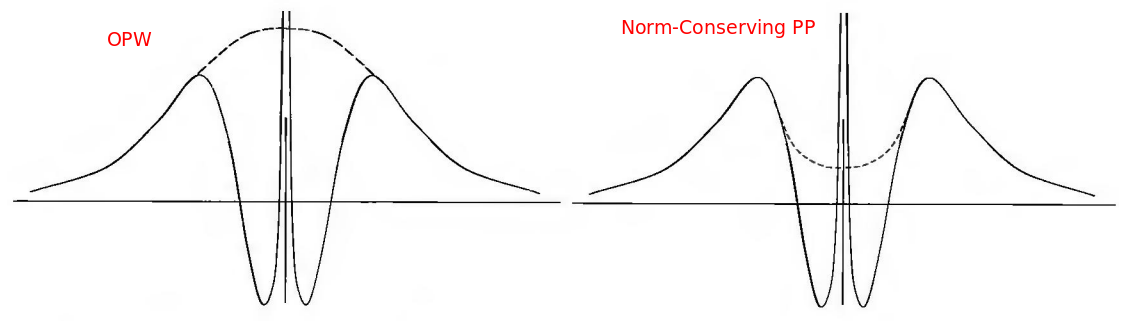
\includegraphics[height=1.30in,width=4.17in,viewport=0 0 1150 350,clip]{Figures/Pseudo-OPW_NCPP.png}
\caption{\small \textrm{Schematic example of a valence function that has the character of a $3s$ orbital near the nucleus and two examples of smooth functions (dashed lines) that equal the full wave-function outside the core region. Left: the smooth part of the valence function defined by OPW-like equation; Right: a smooth pseudo-function that satisfies the norm-conservation condition.}}%(与文献\cite{EPJB33-47_2003}图1对比)
\label{Pseudo-OPW_NCPP}
\end{figure}
}

\frame
{
	\frametitle{赝势去屏蔽与非局域化}
	第一原理赝势建立了赝波函数与对应赝势的一一对应关系,但该赝势包含了电子屏蔽(原子、离子环境)信息,去屏蔽后的赝势对环境依赖更低,“可移植性”更好
	$$V_{\mathrm{ion},l}^{\mathrm{PP}}(r)=V_{\mathrm{src},l}^{\mathrm{PP}}(r)-V_{\mathrm{H},l}^{\mathrm{PP}}(r)-V_{XC,l}^{\mathrm{PP}}(r)$$
	去屏蔽过程中,特别需要注意$V_{XC,l}^{\mathrm{PP}}(r)$的处理
	$$V_{XC}^{\mathrm{PP}}(r)=V_{XC}^{\mathrm{PP}}([n^{\mathrm{PP}}],r)+\big[V_{XC,l}^{\mathrm{PP}}([n^{\mathrm{PP}}+n^{core}],r)-V_{XC}^{\mathrm{PP}}([n^{\mathrm{PP}}],r)\big]$$
	如果定义函数
	$$\chi_{lm}^{\mathrm{PP}}(\vec r)=\bigg\{\varepsilon_l-\bigg[-\dfrac12\nabla^2+V_{local}^{\mathrm{PP}}(\vec r)\bigg]\bigg\}\psi_{lm}^{\mathrm{PP}}(\vec r)$$
	赝势可以分解为局域部分与非局域部分之和
	$$V_{NL}^{\mathrm{PP}}(r)=V_{local}^{\mathrm{PP}}(r)+\dfrac{|\chi_{lm}^{\mathrm{PP}}\rangle\langle\chi_{lm}^{\mathrm{PP}}|}{\langle\chi_{lm}^{\mathrm{PP}}|\psi_{lm}^{\mathrm{PP}}\rangle}=V_{local}^{\mathrm{PP}}(r)+\sum_{lm}\dfrac{|\psi_{lm}^{\mathrm{PP}}\delta V_l\rangle\langle\delta V_l\psi_{lm}^{\mathrm{PP}}|}{\langle\psi_{lm}^{\mathrm{PP}}|\delta V_l|\psi_{lm}^{\mathrm{PP}}\rangle}$$
}

\frame
{
	\frametitle{模守恒赝势构造流程}
\begin{figure}[h!]
\centering
%\vspace*{-0.10in}
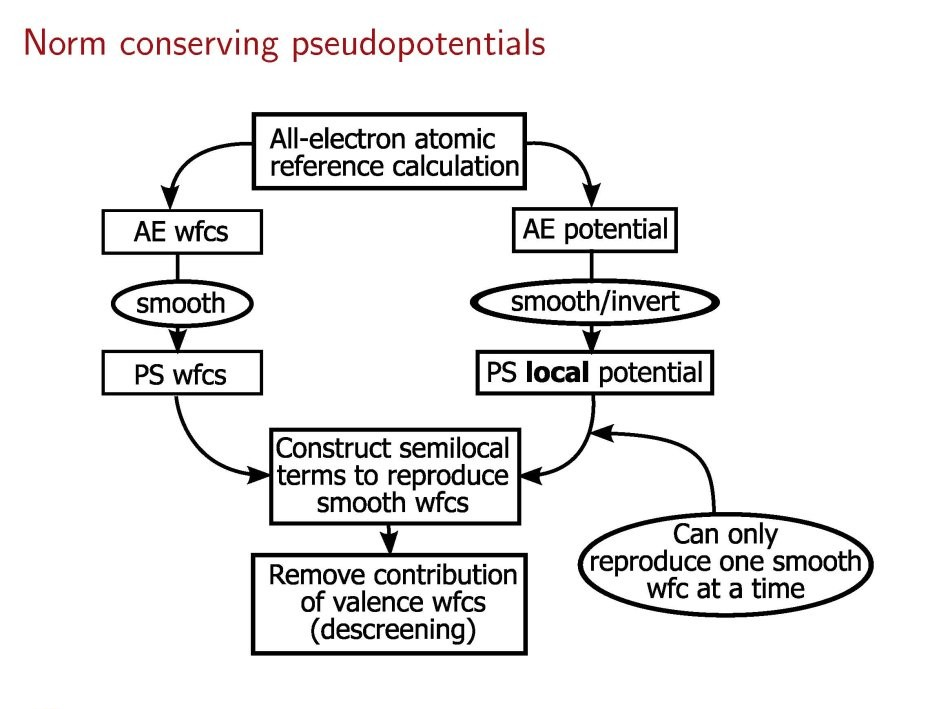
\includegraphics[height=2.70in,width=3.77in,viewport=70 40 900 610,clip]{Figures/Pseudo-NC.jpg}
%\caption{\small \textrm{Pseudopotential for metallic sodium, based on the empty core model and screened by the Thomas-Fermi dielectric function.}}%(与文献\cite{EPJB33-47_2003}图1对比)
\label{Pseudo-NC}
\end{figure}
}

\frame
{
\frametitle{超软赝势}
\begin{itemize}
\setlength{\itemsep}{5pt}
	\item 赝势构造的模守恒条件
%		\begin{displaymath}
%			\int_0^{r_c}\mathrm{d}\vec r\varphi^{\ast PS}(\vec r)\varphi^{PS}(\vec r)=\int_0^{r_c}\mathrm{d}\vec r\varphi^{\ast}(\vec r)\varphi(\vec r)
%		\end{displaymath}
	很好地解决了赝势可移植性问题,但对$1s$、$2p$、$3d$等轨道,模守恒方案构造的赝势过于“硬”,所需平面波基组依然非常大
	\item 超软\textrm{(Ultra-soft)}赝势,解除模守恒条件,实现对第一、第二周期元素的高效计算
\end{itemize}
\begin{figure}[h!]
\vspace*{-0.10in}
\centering
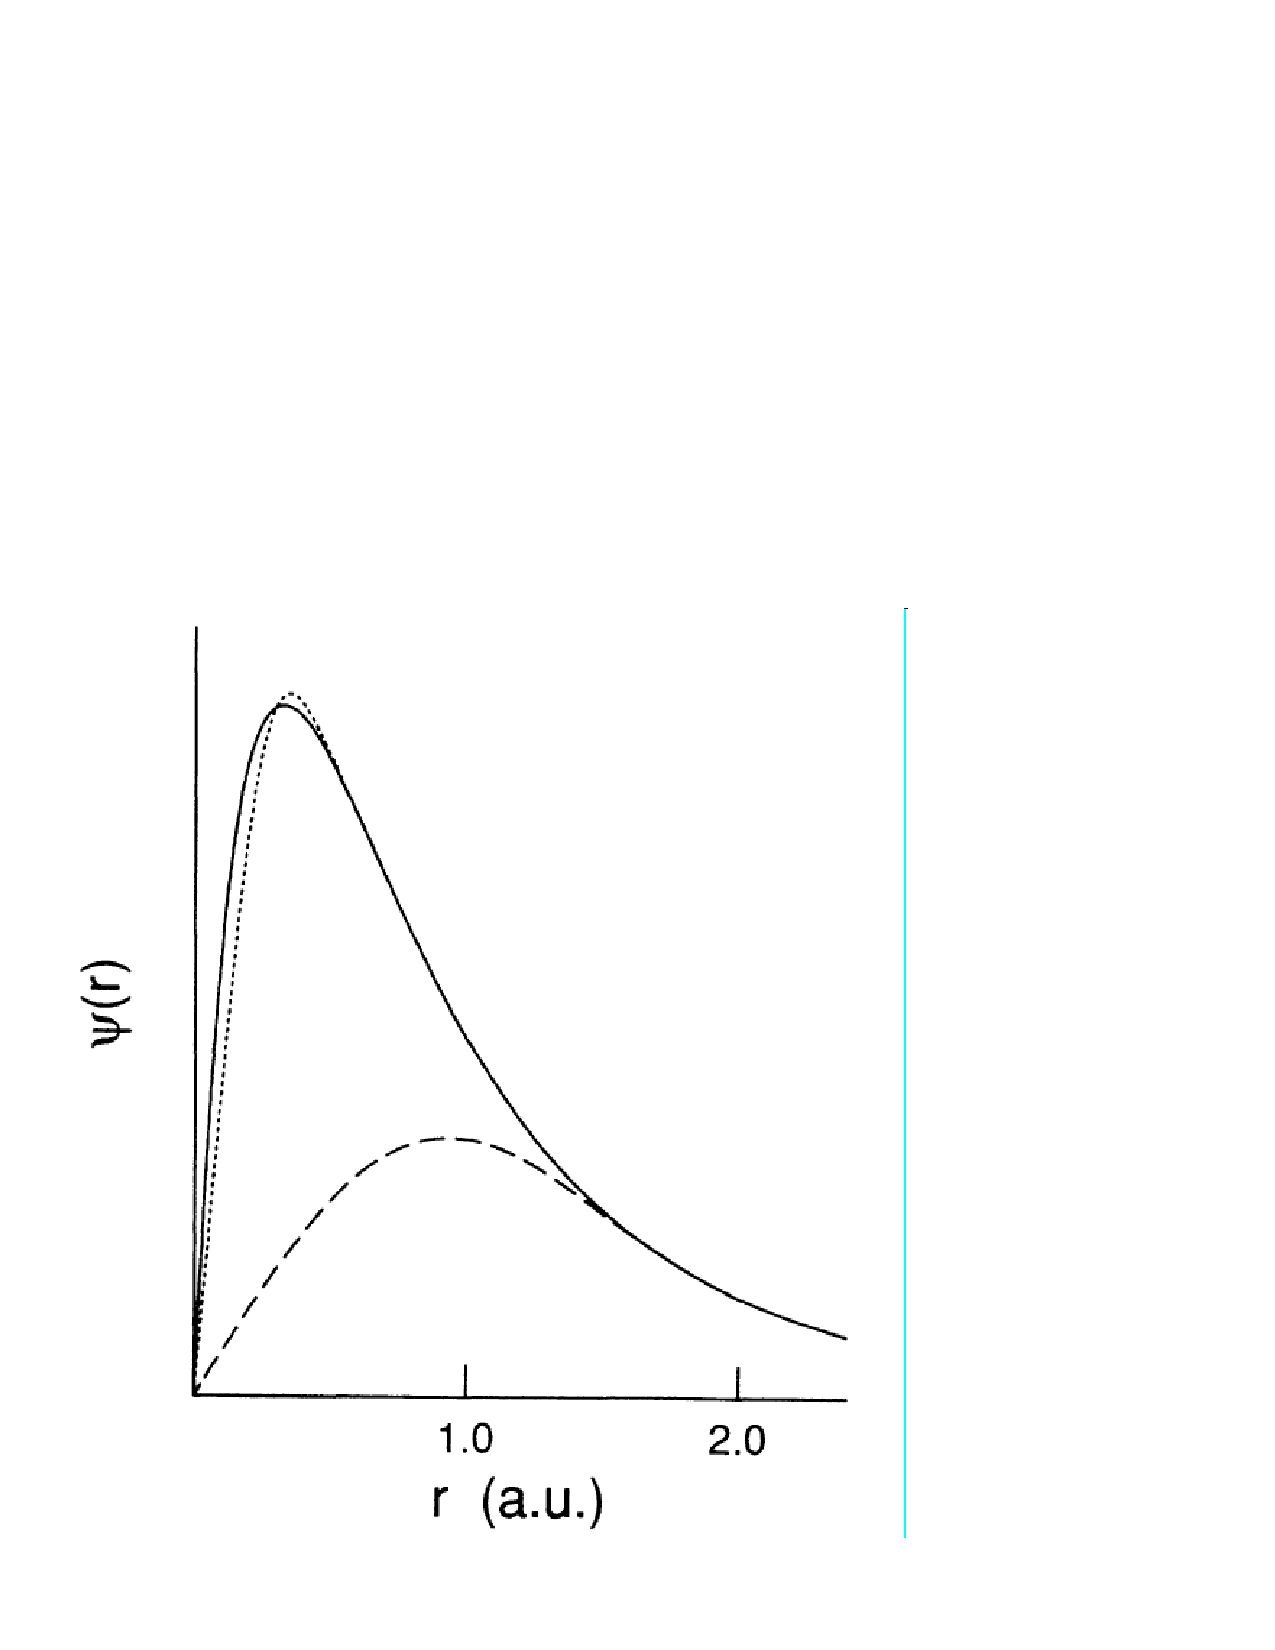
\includegraphics[height=1.35in,width=1.40in,viewport=30 55 415 500,clip]{Figures/Norm-US-wave.pdf}
\caption{\small \textrm{Oxygen 2} \textit{p} \textrm{radical wave function (solid), NC-pseudo-wave (dottde) and US-pseudo-wave (dashed).}}%(与文献\cite{EPJB33-47_2003}图1对比)
\label{Norm-US-wave}
\end{figure}
}

\frame
{
\frametitle{超软赝势的构造}
超软赝势在平缓的局域势函数$V^L(\vec r)$和赝波函数$|\phi_{lmj}(\vec r)\rangle$的基础上,构造函数
\begin{displaymath}
	|\chi_{lmj}(\vec r)\rangle=\bigg[\varepsilon_{lj}-\dfrac12\nabla^2-V^L(\vec r)\bigg]|\phi_{lmj}(\vec r)\rangle
\end{displaymath}
在此基础上得到矩阵$\mathbf{D}_{ij}=\langle\phi_i|\chi_j\rangle$和局域函数
\begin{displaymath}
	|\beta_i\rangle=\sum_j(\mathbf{D}^{-1})_{ji}|\chi_{j}\rangle
\end{displaymath}
因此非局域赝势可以表示为
\begin{displaymath}
	V_{NL}=\dfrac{|\chi_i\rangle\langle\chi_i|}{\langle\chi_i|\phi_i\rangle}=\sum_{i,j}\mathbf{D}_{ij}|\beta_i\rangle\langle\beta_j|
\end{displaymath}
用平缓函数构造赝波函数与真实波函数的电荷密度差
\begin{displaymath}
	Q_{nm}(\vec r)=\varphi_n^{\ast}(\vec r)\varphi_m(\vec r)-\tilde\varphi_n^{\ast}(\vec r)\tilde\varphi_m(\vec r)
\end{displaymath}
}

\frame
{
	\frametitle{超软赝势总能量计算}
	\begin{displaymath}
		\begin{aligned}
			E_{\mathrm{total}}=&\sum_j^{\mathrm{occ}}\langle\phi_{lmj}|\bigg[-\dfrac12\nabla^2+V_{\mathrm{local}}^{\mathrm{ion}}+\sum_{s,s^{\prime}}\mathbf{D}_{s,s^{\prime}}^{\mathrm{ion}}|\beta_s\rangle\langle\beta_{s^{\prime}}|\bigg]|\phi_{lmj}\rangle\\
			&+E_{H}[n_v]+E_{N-N}+E_{XC}[n_v]
		\end{aligned}
	\end{displaymath}
	其中$n_v(\vec r)=\sum\limits_j^{\mathrm{occ}}\phi_{lmj}^{\ast}(\vec r)\phi_{lmj}(\vec r)+\sum\limits_{s,s^{\prime}}\sum\limits_j^{\mathrm{occ}}\langle\phi_{lmj}|\beta_{s^{\prime}}\rangle\langle\beta_s|\phi_{lmj}\rangle Q_{s,s^{\prime}}(\vec r)$
	$$V_{\mathrm{local}}^{\mathrm{ion}}=V_{local}-V_{\mathrm H}-V_{XC}$$
	$$\mathbf{D}_{s,s^{\prime}}^{\mathrm{ion}}=\mathbf{D}_{s,s^{\prime}}-\int\mathrm{d}\vec r\big[V_{\mathrm{H}}(\vec r)+V_{XC}(\vec r)\big]Q_{s,s^{\prime}}(r)$$
	由此可得广义本征值方程
	$$\bigg[-\dfrac12\nabla^2+V_{\mathrm{local}}+V_{NL}^{\mathrm{US}}-\varepsilon_i\bigg(\mathbf{1}+\sum_{s,s^{\prime}}Q_{s,s^{\prime}}|\beta_s\rangle\langle\beta_{s^{\prime}}|\bigg)\bigg]|\phi_{lmi}\rangle=0$$
}

\frame
{
	\frametitle{赝势方法发展概要}
\begin{figure}[h!]
\centering
\vspace*{-0.25in}
%\hspace*{-0.80in}
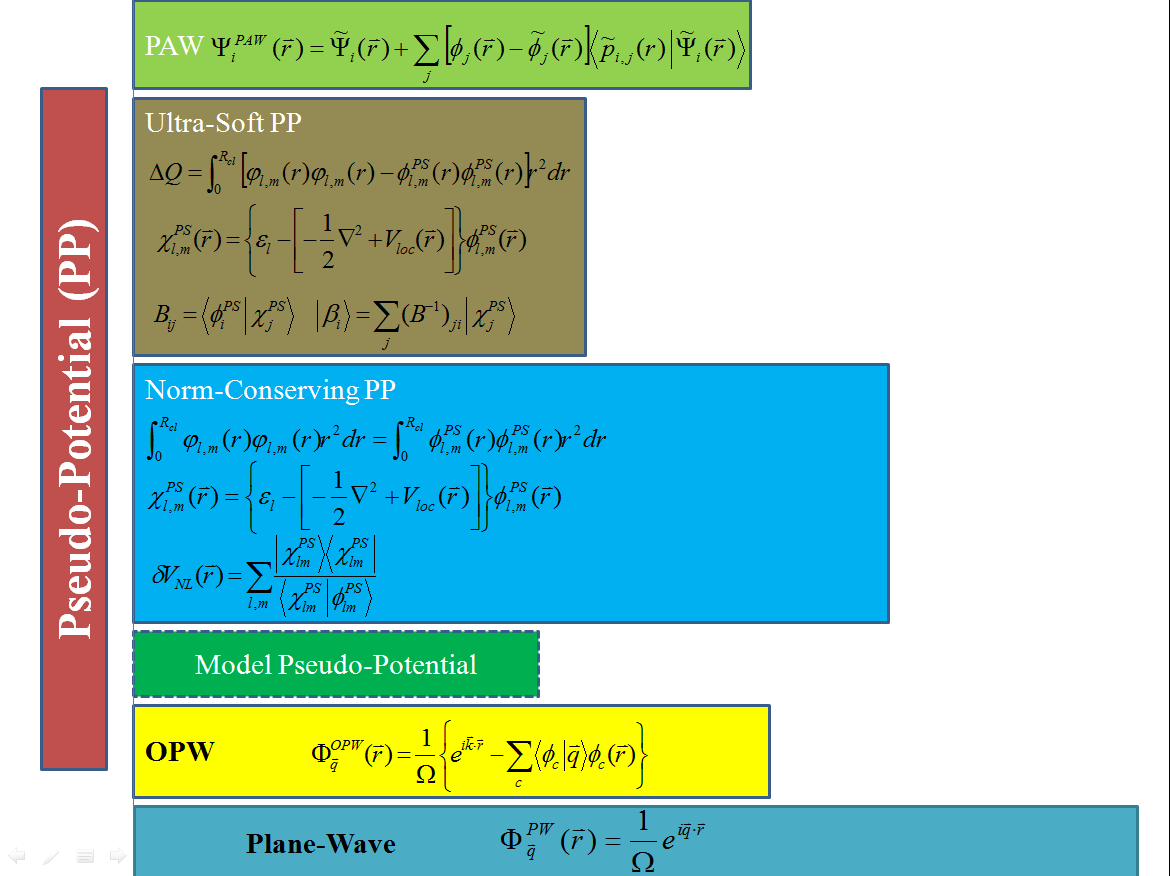
\includegraphics[height=2.80in,width=4.10in,viewport=0 0 1190 875,clip]{Figures/Pseudo_Potential.png}
%\caption{\small \textrm{Pseudopotential for metallic sodium, based on the empty core model and screened by the Thomas-Fermi dielectric function.}}%(与文献\cite{EPJB33-47_2003}图1对比)
\label{Pseudo_Poential}
\end{figure}
}

\subsection{\rm{PAW~}方法概要}
\frame
{
	\frametitle{\textrm{PAW}方法概要}
\begin{itemize}
	\item 与芯层态正交的全部价电子构成的\textrm{Hilbert}空间%,价电子彼此的正交使得波函数在\textrm{Muffin-tin}球内振荡
	\item 作\textcolor{red}{线性空间变换},全电子波函数$|\Psi\rangle$与赝波函数$|\tilde\Psi\rangle$满足:
		$$|\Psi\rangle=\mathbf{\tau|}\tilde\Psi\rangle$$
%	$$\tau=\mathbf{1}+\sum_{\mathrm R}\hat\tau_{\mathrm R}$$
	\item 在原子核附近的$r_c$范围内,波函数用原子分波函数展开:
	$$|\Psi\rangle=|\tilde\Psi\rangle+\sum_i(|\phi_i\rangle-|\tilde\phi_i\rangle)\langle\tilde p_i|\tilde\Psi\rangle$$
	\item 在$r_c$外$|\tilde\Psi\rangle$与$|\Psi\rangle$变换前后保持不变,因此线性变换$\mathbf{\tau}$可表示为:
	$$\mathbf{\tau}=\mathbf{1}+\sum_i(|\phi_i\rangle-|\tilde\phi_i\rangle)\langle\tilde p_i|$$
\end{itemize}
其中$|\tilde p_i\rangle$是\textrm{MT}球内的投影函数\\
$i$表示原子位置$\vec R$、原子轨道($l,m$)和能级$\epsilon_k$的指标。
}

\frame
{
	\frametitle{\textrm{PAW}方法的基本思想}
	\vspace{10pt}
\begin{figure}[h!]
\centering
\includegraphics[height=1.8in,width=4.in,viewport=30 210 570 440,clip]{Figures/PAW_projector.eps}
\caption{\small \textrm{The analysis of PAW basic function.}}%(与文献\cite{EPJB33-47_2003}图1对比)
\label{PAW_baisc}
\end{figure}
}

\frame
{
\frametitle{\textrm{PAW}方法的基本思想}
	在赝波函数$|\tilde\Psi\rangle$表象下,算符期望值计算满足$$\langle A \rangle=\langle\Psi|\mathbf{A}|\Psi\rangle=\langle\tilde\Psi|\mathbf{\tau}^{\dag}\mathbf{A}\mathbf{\tau}|\tilde\Psi\rangle=\langle\tilde\Psi|\tilde{\mathrm{A}}|\tilde\Psi\rangle$$
\begin{itemize}
	\item 一般赝算符$\tilde A$表示为
		$$\tilde A=\mathbf{A}+\sum_i|\tilde p_i\rangle(\langle\phi_i|\mathbf{A}|\phi_i\rangle-\langle\tilde\phi_i|\mathbf{A}|\tilde\phi_i\rangle)\langle\tilde p_i|$$
	\item 赝重叠算符$\tilde O$表示为
		$$\tilde O=\mathbf{1}+\sum_i|\tilde p_i\rangle(\langle\phi_i|\phi_i\rangle-\langle\tilde\phi_i|\tilde\phi_i\rangle)\langle\tilde p_i|$$
\end{itemize}
}

\frame
{
\frametitle{\textrm{PAW}方法密度计算}
在\textrm{PAW}框架下,将密度算符$|\vec r\rangle\langle\vec r|$代入,可知密度表达式为
$$n(\vec r)=\tilde n(\vec r)+n^1(\vec r)-\tilde n^1(\vec r)$$
这里
$$\tilde n(\vec r)=\sum_nf_n\langle\tilde\Psi_n|\vec r\rangle\langle\vec r|\tilde\Psi_n\rangle$$ 
$$n^1(\vec r)=\sum_{n,(i,j)}f_n\langle\tilde\Psi_n|\tilde p_i\rangle\langle\phi_i|\vec r\rangle\langle\vec r|\phi_j\rangle\langle\tilde p_j|\tilde\Psi_n\rangle$$
$$\tilde n^1(\vec r)=\sum_{n,(i,j)}f_n\langle\tilde\Psi_n|\tilde p_i\rangle\langle\tilde\phi_i|\vec r\rangle\langle\vec r|\tilde\phi_j\rangle\langle\tilde p_j|\tilde\Psi_n\rangle$$
}

\frame
{
\frametitle{\textrm{PAW}方法总能量的计算}
总能量泛函
%\begin{displaymath}
%	\begin{aligned}
%		E&=\sum_nf_n\langle\Psi_n|-\dfrac12\nabla^2|\Psi_n\rangle\\
%		 &+\dfrac12\int\mathrm{d}\vec r\int\mathrm{d}\vec r^{\prime}\dfrac{(n+n^Z)(n+n^Z)}{|\vec r-\vec r^{\prime}|}+\int\mathrm{d}\vec r n\epsilon_{\mathrm{XC}}(n)
%	\end{aligned}
%\end{displaymath}
$E=\tilde E+E^1-\tilde E^1$,每一项分别表示为:
\begin{displaymath}
	\begin{aligned}
		\tilde E&=\sum_nf_n\langle\tilde\Psi_n|-\dfrac12\nabla^2|\tilde\Psi_n\rangle\\
		 &+\dfrac12\int\mathrm{d}\vec r\int\mathrm{d}\vec r^{\prime}\dfrac{(\tilde n+\hat n)(\tilde n+\hat n)}{|\vec r-\vec r^{\prime}|}+\int\mathrm{d}\vec r \tilde n\bar v+\int\mathrm{d}\vec r \tilde n\epsilon_{\mathrm{XC}}(\tilde n)
 	\end{aligned}
\end{displaymath}
\begin{displaymath}
	\begin{aligned}
		E^1&=\sum_{n,(i,j)}f_n\langle\tilde\Psi_n|\tilde p_i\rangle\langle\phi_i|-\dfrac12\nabla^2|\phi_j\rangle\langle\tilde p_j|\tilde\Psi_n\rangle\\
		 &+\dfrac12\int\mathrm{d}\vec r\int\mathrm{d}\vec r^{\prime}\dfrac{(n^1+n^Z)(n^1+n^Z)}{|\vec r-\vec r^{\prime}|}+\int\mathrm{d}\vec r n^1\epsilon_{\mathrm{XC}}(n^1)
 	\end{aligned}
\end{displaymath}
\begin{displaymath}
	\begin{aligned}
		\tilde E^1&=\sum_{n,(i,j)}f_n\langle\tilde\Psi_n|\tilde p_i\rangle\langle\tilde\phi_i|-\dfrac12\nabla^2|\tilde\phi_j\rangle\langle\tilde p_j|\tilde\Psi_n\rangle\\
		 &+\dfrac12\int\mathrm{d}\vec r\int\mathrm{d}\vec r^{\prime}\dfrac{(\tilde n^1+\hat n)(\tilde n^1+\hat n)}{|\vec r-\vec r^{\prime}|}+\int\mathrm{d}\vec r \tilde n^1\bar v+\int\mathrm{d}\vec r \tilde n^1\epsilon_{\mathrm{XC}}(\tilde n^1)
 	\end{aligned}
\end{displaymath}
}

%\subsection{\rm{PAW}的实现}
\frame
{
	\frametitle{补偿电荷的表示}
	补偿电荷$\hat n$要求局域在缀加区(\textrm{Augmentation region}),可表示为
	$$\hat n=\sum_R\hat n_R$$
	其中$\hat n_R$是单个原子截断区间的补偿电荷,可以表示为广义的\textrm{Gaussian}函数的求和
	$$\hat n_R(r)=\sum_{L=(l,m)}g_{RL}(r)Q_{RL}$$
	其中$g_{RL}(r)$表示为
	$$g_{RL}(r)=C_l|r-R|^lY_L(r-R)\mathrm{e}^{-(|r-R|/r_c)^2}$$
	系数$C_l$是归一化系数,由条件
	$\int\mathrm{d}rr^lY_L(r)g_L(r)=1$
	确定

	$Q_{RL}$是补偿电荷要满足的多极矩
	$$Q_{RL}=\int\mathrm{d}r|r-R|^l\big[n_R^1(r)+n_R^Z(r)-\tilde n_R^1(r)\big]Y_L^{\ast}(r-R)$$
}

\frame
{
	\frametitle{补偿电荷与能量$\tilde E$}
	如果要求\textrm{Gaussian}函数在缀加区衰减,则需要用很高的\textrm{Fourier}截断,这意味着需要很高的平面波能量截断。引入补偿电荷$\hat n^{\prime}$,要求满足条件
	\begin{itemize}
		\item $\hat n^{\prime}$与$\hat n$具有相同的多极矩
		\item $\hat n^{\prime}$对应的\textrm{Gaussian}函数的衰减半径$r_c^{\prime}$比$r_c$大得多,可以用很少的平面波展开
	\end{itemize}
	因此能量$\tilde E$中的\textcolor{blue}{静电相互作用}可以表示为
	\begin{displaymath}
		\begin{aligned}
			&\dfrac12\int\mathrm{d}r\int\mathrm{d}r^{\prime}\dfrac{(\tilde n+\hat n)(\tilde n+\hat n)}{|r-r^{\prime}|}\\
			=&\underline{\dfrac12\int\mathrm{d}r\int\mathrm{d}r^{\prime}\dfrac{(\tilde n+\hat n^{\prime})(\tilde n+\hat n^{\prime})}{|r-r^{\prime}|}}
			+\underline{\int\mathrm{d}r\tilde n(r)\hat v(r)}+\underline{\sum_{R,R^{\prime}}U_{R,R^{\prime}}}
		\end{aligned}
	\end{displaymath}
}

\frame
{
	\frametitle{能量$\tilde E$的静电相互作用分解}
	其中第一项是平滑函数,可以在\textrm{Fourier}空间计算
	$$2\pi V\sum_G\dfrac{|\tilde n(G)+\hat n^{\prime}(G)|^2}{G^2}$$
	第二项的$\hat v(r)$表示为
	$$\hat v(r)=\int\mathrm{d}r^{\prime}\dfrac{\hat n(r^{\prime})-\hat n^{\prime}(r^{\prime})}{|r-r^{\prime}|}$$
	虽然$\hat v(r)$和$n(r)$一样有高\textrm{Fourier}截断,但\textcolor{red}{高阶部分不会对$\int\mathrm{d}r\tilde n(r)\hat v(r)$有贡献}

	最后一项中$U_{R,R^{\prime}}$是原子间的短程成对势
	$$U_{R,R^{\prime}}=\dfrac12\int\mathrm{d}r\int\mathrm{d}r^{\prime}\dfrac{\hat n_R(r)\hat n_{R^{\prime}}(r^{\prime})-\hat n_R^{\prime}(r)\hat n_{R^{\prime}}^{\prime}(r^{\prime})}{|r-r^{\prime}|}$$
	这一项\textcolor{blue}{可以通过\textrm{Ewald}求和方法计算}
}

\frame
{
	\frametitle{重叠矩阵和\textrm{Hamiltonian}矩阵}
重叠算符:
$$\tilde O=1+\sum_{i,j}|\tilde p_i\rangle\bigg[\langle\phi_i|\phi_j\rangle-\langle\tilde\phi_i|\tilde\phi_j\rangle\bigg]\langle\tilde p_j|$$
\textrm{Hamilitonian}算符:
%\begin{itemize}
%	\item 动能算符:
%		$$\tilde T=-\dfrac12\nabla^2+\sum_{i,j}|\tilde p_i\rangle[\langle\phi_i|-\dfrac12\nabla^2|\phi_j\rangle-\langle\tilde\phi_i|-\dfrac12\nabla^2|\tilde\phi_j\rangle]\langle\tilde p_j|$$
%	\item 完全势\textrm{(full-potential)}算符:
%$$v(\vec r)=\tilde v(\vec r)+v^1(\vec r)-\tilde v^1(\vec r)$$
%	\item \textrm{Hamilton}算符:
\begin{displaymath}
	\begin{aligned}
		\tilde H=&-\dfrac12\nabla^2+\tilde v+\sum_{i,j}|\tilde p_i\rangle\bigg[\langle\phi_i|-\dfrac12\nabla^2+v^1|\phi_j\rangle\\
			&-\langle\tilde\phi_i|-\dfrac12\nabla^2+\tilde v^1|\tilde\phi_j\rangle\bigg]\langle\tilde p_j| 
	\end{aligned}
\end{displaymath}
%\end{itemize}
	完整的势函数\textrm{(full-potential)}算符:
$$v(\vec r)=\tilde v(\vec r)+v^1(\vec r)-\tilde v^1(\vec r)$$
因此可以有
$$\left.\dfrac{\partial E[\tilde\Psi, R]}{\partial\langle\tilde\Psi_n|}\right|_R=\tilde H|\tilde\Psi_n\rangle f_n$$
}

\frame
{
	\frametitle{\textrm{PAW}原子数据集}
\textrm{PAW}原子数据集是在原子核附近$r_c$范围内将波函数用原子分波展开所需信息的统称,是\textrm{PAW}计算的基础。

\textrm{PAW}原子数据集主要包括
	\begin{itemize}
		\item 分波信息:原子分波$\phi_i$、赝分波$\tilde\phi_i$和投影子波函数$p_i$
		\item 密度信息:$r_c$内的电荷密度$n^1$、赝电荷密度$\tilde n^1$和补充电荷$\hat n$
		\item 赝势信息:局域赝势$\tilde v_{loc}(\vec r)$
	\end{itemize}
	与赝势方法相似,一套原子数据集将用于各种化学环境下的\textrm{PAW}计算,即要求原子数据集有良好的可移植性;与赝势方法不同之处在于\textrm{PAW}原子集中除了赝原子的信息,还包含了真实原子的信息。
}

\frame
{
	\frametitle{\textrm{PAW}原子数据集}
	原子分波:$$\bigg(-\dfrac12\nabla^2+v_{at}-\varepsilon_i^1\bigg)|\phi_i\rangle=0$$
	赝原子分波:$$\bigg(-\dfrac12\nabla^2+w_i(r)-\varepsilon_i^1\bigg)|\tilde\phi_i\rangle=0$$
	局域赝势:%$$w_i(r)=\tilde v_{at}(r)+c_ik(r)=\tilde v_{at}(0)\mathrm{e}^{-(r/r_k)^{\lambda}}+[1-k(r)]v_{at}(r)+c_i\mathrm{e}^{-(r/r_k)^{\lambda}}$$
	$$w_i(r)=\tilde v_{at}(0)\mathrm{e}^{-(r/r_k)^{\lambda}}+[1-\mathrm{e}^{-(r/r_k)^{\lambda}}]v_{at}(r)+c_i\mathrm{e}^{-(r/r_k)^{\lambda}}$$
\begin{figure}[h!]
\centering
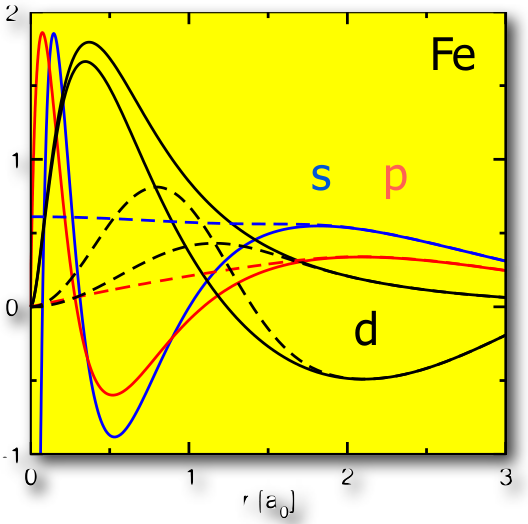
\includegraphics[height=1.2in,width=1.5in,viewport=0 0 570 545,clip]{Figures/PAW-partical.png}
\caption{\small \textrm{The partical-wave of Fe atom.}}%(与文献\cite{EPJB33-47_2003}图1对比)
\label{PAW_partical_Fe}
\end{figure}
}

\frame
{
	\frametitle{\textrm{PAW projector}}
	投影函数:$$|\tilde p_i\rangle=\bigg(-\dfrac12\nabla^2+\tilde v_{at}-\varepsilon_i^1\bigg)|\tilde\phi_i\rangle$$
	\textrm{Gram-Schmidt}正交化
	$$|\tilde p_i\rangle=|\tilde p_i\rangle-\sum_{j=1}^{i-1}|\tilde p_j\rangle\langle\tilde\phi_j|\tilde p_i\rangle$$
%	$$|\phi_i\rangle=|\phi_i\rangle-\sum_{j=1}^{i-1}|\phi_j\rangle\langle\tilde p_j|\tilde\phi_i\rangle$$
%	$$|\tilde\phi_i\rangle=|\tilde\phi_i\rangle-\sum_{j=1}^{i-1}|\tilde\phi_j\rangle\langle\tilde p_j|\tilde\phi_i\rangle$$
	$|\phi_i\rangle=|\phi_i\rangle-\sum\limits_{j=1}^{i-1}|\phi_j\rangle\langle\tilde p_j|\tilde\phi_i\rangle\quad|\tilde\phi_i\rangle=|\tilde\phi_i\rangle-\sum\limits_{j=1}^{i-1}|\tilde\phi_j\rangle\langle\tilde p_j|\tilde\phi_i\rangle$
\begin{figure}[h!]
\centering
\vspace*{-0.4in}
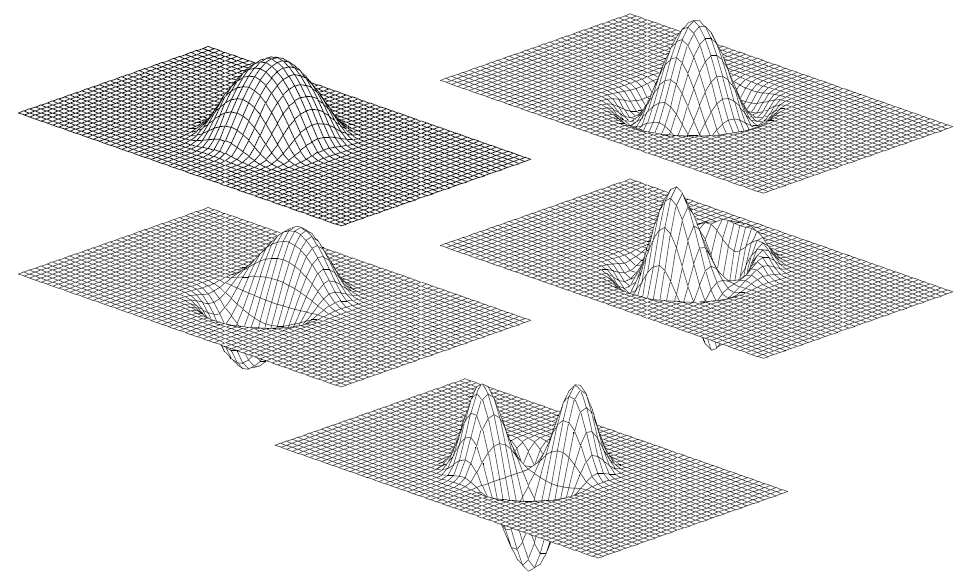
\includegraphics[height=1.5in,width=2.3in,viewport=0 0 1100 745,clip]{Figures/PAW_projector-2.png}
\caption{\small \textrm{The projector of PAW.}}%(与文献\cite{EPJB33-47_2003}图1对比)
\label{PAW_projector}
\end{figure}
\begin{itemize}
	\item 与分波具有相同的角动量$l$
	\item 局域在缀加区域(Augmentation region)
	\item 节点依次增加
\end{itemize}
}

\frame
{
	\frametitle{\textrm{局域势$\bar v$}}
	去屏蔽局域势:$$\bar v(r)=\tilde v_{at}(r)-\int\mathrm{d}r^{\prime}\dfrac{\tilde n(r^{\prime})+\hat n(r^{\prime})}{|r-r^{\prime}|}-\mu_{xc}[\tilde n(r)]$$
	其中$\tilde v_{at}(r)$的确定
	$$\bigg[-\dfrac12\nabla^2+\tilde v_{at}-\varepsilon+\sum_{(i,j)}|\tilde p_i\rangle\big(\mathrm{d}H_{ij}-\varepsilon\mathrm{d}O_{ij}\big)\langle\tilde p_j|\bigg]|\tilde\Psi_j\rangle=0$$
	其中$\mathrm{d}H_{ij}$和$\mathrm{d}O_{ij}$分别是
	$$\mathrm{d}H_{ij}=\langle\phi_i|-\dfrac12\nabla^2+v_{at}|\phi_j\rangle-\langle\tilde\phi_i|-\dfrac12\nabla^2+\tilde v_{at}|\tilde\phi_j\rangle$$
	$$\mathrm{d}O_{ij}=\langle\phi_i|\phi_j\rangle-\langle\tilde\phi_i|\tilde\phi_j\rangle$$
}

\frame
{
	\frametitle{\textrm{局域势$\bar v$}}
	如果解$$|\tilde\Psi\rangle=|u\rangle+\sum_i|w_i\rangle c_i$$
	其中$|u\rangle$和$|w_i\rangle$的定义分别为
	$$\big(-\frac12\nabla^2+\tilde v-\varepsilon\big)|u\rangle=0$$
	$$\big(-\frac12\nabla^2+\tilde v-\varepsilon\big)|w_i\rangle=|\tilde p_i\rangle$$
	因此可以得到
	$$c_i=-\sum_{j,l}\bigg[\delta_{ij}+\sum_k\mathrm{d}H_{ik}-\varepsilon\mathrm{d}O_{ik}\langle\tilde p_k|w_j\rangle\bigg]^{-1}\big(\mathrm{d}H_{jl}-\varepsilon\mathrm{d}O_{jl}\big)\langle p_l|u\rangle$$
}

%\frame
%{
%%	\frametitle{\textrm{PAW}原子数据集}
%	\frametitle{\textrm{PAW Augmentation}}
%\begin{figure}[h!]
%\centering
%\includegraphics[height=2.3in,width=4.0in,viewport=0 0 1280 745,clip]{Figures/PAW-baseset.png}
%\caption{\small \textrm{The Augmentation of PAW.}}%(与文献\cite{EPJB33-47_2003}图1对比)
%\label{PAW_baiseset}
%\end{figure}
%}

%\frame
%{
%	\frametitle{\textrm{PAW Augmentation}}
%\begin{figure}[h!]
%\centering
%\includegraphics[height=2.3in,width=4.0in,viewport=0 0 1100 745,clip]{Figures/PAW-projector.png}
%\caption{\small \textrm{The projector of PAW.}}%(与文献\cite{EPJB33-47_2003}图1对比)
%\label{PAW_projector}
%\end{figure}
%}

\subsection{基态总能量表达式}
\frame
{
	\frametitle{晶体总能量的一般表示}
采用赝势方法计算的晶体总能量$E_T$由晶格中的电子能量$E_{e-e}$与离子实排斥能$E_{N-N}$之和:
	\begin{displaymath}
		E_T=E_{e-e}+E_{N-N}=T[\rho]+E_{ext}+E_{\mathrm{Coul}}+E_{\mathrm{XC}}+E_{N-N}
	\end{displaymath}
根据\textrm{Kohn-Sham}方程,其中动能泛函用单电子能量表示为
\begin{displaymath}
	T[{\rho}]=\sum_in_i\langle\psi_i|\varepsilon_i-V_{\mathrm{KS}}|\psi_i\rangle
\end{displaymath}
$n_i$是$\psi_i$上的电子占据数,$\varepsilon_i$是其能量本征值,因此有
\begin{displaymath}
	\hspace*{-12.0pt}	E_T=\sum_in_i\varepsilon_i-\dfrac12\int\int\mathrm{d}\vec r\mathrm{d}\vec r\dfrac{\rho(\vec r)\rho(\vec r^{\prime})}{|\vec r-\vec r^{\prime}|}+\int\mathrm{d}\vec r\rho(\vec r)[\epsilon_{\mathrm{XC}}(\vec r)-V_{\mathrm{XC}}(\vec r)]+E_{N-N}
\end{displaymath}
}

\frame
{
	\frametitle{晶体总能量倒空间的表示}
周期体系的总能量表达式在动量空间($\vec K$空间)计算更方便
\begin{displaymath}
	\hspace*{-15.0pt}	E_T=\textcolor{red}{\sum_in_i\varepsilon_i}-\dfrac{\Omega}2\sum_{\textcolor{red}{\vec k\neq 0}}\rho^{\ast}(\vec k)V_{\mathrm{Coul}}(\vec k)+\Omega\sum_{\vec k}\rho^{\ast}(\vec k)[\epsilon_{\mathrm{XC}}(\vec k)-V_{\mathrm{XC}}(\vec k)]+E_{N-N}
\end{displaymath}
其中$V_{\mathrm{Coul}}(\vec k)$、$\epsilon_{\mathrm{XC}}(\vec k)$与$\rho^{\ast}(\vec k)$分别是\textrm{Coulomb}相互作用、单个电子的交换-相关能、交换-相关势和电子密度的\textrm{Fourier}分量。

由\textrm{Poisson}方程
\begin{displaymath}
	\nabla^2V_{\mathrm{Coul}}(\vec r)=-4\pi\rho(\vec r)
\end{displaymath}
的\textrm{Fourier}展开有
\begin{displaymath}
	V_{\mathrm{Coul}}(\vec k)=\dfrac{4\pi\rho^{\ast}(\vec k)}{|\vec k|^2}
\end{displaymath}
交换-相关势和交换-相关能的计算一般先在实空间计算$\epsilon_{\mathrm{XC}}(\vec r)$和$V_{\mathrm{XC}}(\vec r)$后,再通过\textrm{Fourier}变换到动量空间,得到$\epsilon_{\mathrm{XC}}(\vec k)$和$V_{\mathrm{XC}}(\vec k)$
}

\frame
{
	\frametitle{晶体离子相互作用的计算}
	离子间\textrm{Coulomb}相互作用能之和
	\begin{displaymath}
		E_{N-N}=\dfrac12\sum_{\vec R,s}\sideset{}{^{\prime}}\sum_{\vec R^{\prime},\vec s^{\prime}}\dfrac{Z_sZ_{s^{\prime}}}{|\vec R+\vec r_s-\vec R^{\prime}-\vec r_s^{\prime}|}
	\end{displaymath}
	这里$Z_s$是离子实的电荷数,$\vec R$表示晶格点的位矢,$\vec r_s$代表元胞内原子的相对位矢。

	\textcolor{red}{\textbf{注意}}:~$E_{N-N}$求和包含无穷多项,是发散的;$V_{\mathrm{Coul}}(\vec k=0)$是发散的。
	
	$V_{ext}$在不存在其他外场时,一般只考虑离子-电子的\textrm{Coulomb}相互作用,
	\begin{displaymath}
		\begin{aligned}
			V_{ext}(\vec r)&=\sum_{\vec R,s}\dfrac{-Z_s}{|\vec r-\vec R-\vec r_s|}\\
			&\equiv\sum_{\vec R,s}v_{ext}^s(\vec r-\vec R-\vec r_s)
		\end{aligned}
	\end{displaymath}
}

\frame
{
	\frametitle{晶体总能量计算的奇点排除}
	$V_{ext}$的\textrm{Fourier}分量在$\vec k=0$\textcolor{red}{也是发散的}。这三项单独都是发散的,但因为整个体系出于电中性,所以这些发散项相互抵消,是一个常数。

	因此求解\textrm{Kohn-Sham}方程时,先将$V_{\mathrm{Coul}}(\vec k=0)$和$V_{ext}(\vec k=0)$同时置为零,这相当于\textcolor{red}{将势能作一平移,或者说重新定义势能零点,而在总能量计算中补偿这一平移。}

	发散项之和为:
	\begin{displaymath}
		\begin{aligned}
			\lim_{\vec k\rightarrow0}\Omega&\bigg[\dfrac12V_{\mathrm{Coul}}(\vec k)+\sum_sv_{ext}^s(\vec k)\bigg]\rho^{\ast}(\vec k)+\dfrac12\sum_{\vec R,s}\sideset{}{^{\prime}}\sum_{\vec R^{\prime},\vec s^{\prime}}\dfrac{Z_sZ_{s^{\prime}}}{|\vec R+\vec r_s-\vec R^{\prime}-\vec r_s^{\prime}|}\\
			=&\sum_s\alpha_s\sum_sZ_s+E_{\mathrm{Ewald}}
		\end{aligned}
	\end{displaymath}
}

\frame
{
	\frametitle{发散项的处理}
	对于形如$Z_s/r$的外场,其\textrm{Fourier}分量在$\vec k=0$附近展开
	\begin{displaymath}
		v_{ext}^s(\vec k)=-\dfrac{4\pi Z_s}{\Omega|\vec k|^2}+\alpha_s+O(\vec k); 
	\end{displaymath}
	展开$\rho^{\ast}(\vec k)$,有
	\begin{displaymath}
		\lim_{\vec k\rightarrow 0}\rho^{\ast}(\vec k)=\dfrac{\sum_sZ_s}{\Omega}+\beta|\vec k|^2+O(\vec k)
	\end{displaymath}
去掉高次项,有
\fontsize{8.5pt}{5.2pt}\selectfont{
\begin{displaymath}
	\begin{aligned}
		\lim_{\vec k\rightarrow 0}&\bigg[\boxed{\textcolor{blue}{\dfrac{\Omega}2\dfrac{4\pi[\rho^{\ast}(\vec k)]^2}{|\vec k|^2}}}+\boxed{\Omega}\bigg(\boxed{\textcolor{blue}{-\dfrac{4\pi\sum_sZ_s}{\Omega|\vec k|^2}}}+\sum_s\alpha_s\bigg)\boxed{\rho^{\ast}(\vec k)}+\boxed{\textcolor{red}{\dfrac12\dfrac{4\pi(\sum_sZ_s)^2}{\Omega|\vec k|^2}}}\bigg]\\
		&+\boxed{\dfrac12\sum_{\vec R,s}\sideset{}{^{\prime}}\sum_{\vec R^{\prime},\vec s^{\prime}}\dfrac{Z_sZ_{s^{\prime}}}{|\vec R+\vec r_s-\vec R^{\prime}-\vec r_{s^{\prime}}|}-\lim_{\vec k\rightarrow0}\textcolor{red}{\dfrac12\dfrac{4\pi(\sum_sZ_s)^2}{\Omega|\vec k|^2}}}\\
		=&\sum_s\alpha_s\sum_sZ_s+\textcolor{magenta}{E_{\mathrm{Ewald}}}
	\end{aligned}
\end{displaymath}}
}

\frame
{
	\frametitle{离子间相互作用的\textrm{Ewald}求和}
	\begin{displaymath}
		\begin{aligned}
			E_{\textrm{Ewald}}=&\dfrac12\sum_{\vec R,s}\sideset{}{^{\prime}}\sum_{\vec R^{\prime},\vec s^{\prime}}\dfrac{Z_sZ_{s^{\prime}}}{|\vec R+\vec r_s-\vec R^{\prime}-\vec r_{s^{\prime}}|}-\lim_{\vec k\rightarrow0}\dfrac12\times\dfrac{4\pi(\sum_sZ_s)^2}{\Omega|\vec k|^2}\\
			=&\dfrac12\sum_{\vec R,s}\sideset{}{^{\prime}}\sum_{\vec R^{\prime},\vec s^{\prime}}\dfrac{Z_sZ_{s^{\prime}}}{|\vec R+\vec r_s-\vec R^{\prime}-\vec r_{s^{\prime}}|}-\dfrac1{2\Omega}\sum_{s,s^{\prime}}\int\mathrm{d}\vec r\dfrac{Z_sZ_{s^{\prime}}}r\\
			=&\sum_{s,s^{\prime}}Z_sZ_{s^{\prime}}\bigg\{\dfrac{2\pi}{\Omega}\sum_{\vec k\neq 0}\cos[\vec k\cdot(\vec r_s-\vec r_{s^{\prime}})]\dfrac{\mathrm{e}^{-|\vec k|^2/4\eta^2}}{|\vec k|^2}\\
			&-\dfrac{\pi}{2\eta^2\Omega}+\dfrac14\sum_{\vec R}\dfrac{\mathrm{erf}(\eta x)}x\bigg|_{\vec R+\vec r_s-\vec r_s^{\prime}\neq0}-\dfrac{\eta}{\sqrt{\pi}}\delta_{s,s^{\prime}}\bigg\}
		\end{aligned}
	\end{displaymath}
	$\mathrm{erf}(x)$是误差函数,$\eta$原则上是任意参数。$\alpha_s$由$v_{ext}^s(\vec r)$确定:
	\begin{displaymath}
		\alpha_s=\lim_{\vec k\rightarrow0}\bigg[v_{ext}^s(\vec k)+\dfrac{4\pi Z_s}{\Omega|\vec k|^2}\bigg]=\dfrac1{\Omega}\int\mathrm{d}\vec r\bigg[v_{ext}^s(\vec r)+\dfrac{Z_s}r\bigg]
	\end{displaymath}
}

\frame
{
	\frametitle{总能量表达式}
\fontsize{6.5pt}{4.2pt}\selectfont{
由此得到的总能量表达式是
\begin{displaymath}
	\begin{aligned}
		E_T=&\sum_i\varepsilon_i-\dfrac{\Omega}2\sum_{\vec k\neq0}\rho^{\ast}(\vec k)V_{\mathrm{Coul}}(\vec k)\\
		&+\Omega\sum_{\vec k}\rho^{\ast}(\vec k)[\epsilon_{\mathrm{XC}}(\vec k)-V_{\mathrm{XC}}(\vec k)]\\
		&+\sum_s\alpha_s\sum_sZ_s+E_{\mathrm{Ewald}}
	\end{aligned}
\end{displaymath}
}
\begin{figure}[h!]
\centering
\vspace*{-0.18in}
\includegraphics[height=1.85in,width=2.2in,viewport=0 0 600 495,clip]{Figures/VASP_Total_ENE.png}
\caption{\small \textrm{The Total-E calculated by VASP.}}%(与文献\cite{EPJB33-47_2003}图1对比)
\label{TOTEN_VASP}
\end{figure}
}

\section{\rm{VASP~}软件中\rm{PAW~}计算的实现}
\frame
{
%	\frametitle{\textrm{PAW}原子数据集}
	\frametitle{\textrm{PAW Augmentation}}
\begin{figure}[h!]
\centering
\includegraphics[height=2.3in,width=4.0in,viewport=0 0 1280 745,clip]{Figures/PAW-baseset.png}
\caption{\small \textrm{The Augmentation of PAW.}}%(与文献\cite{EPJB33-47_2003}图1对比)
\label{PAW_baiseset}
\end{figure}
}

%\frame
%{
%	\frametitle{\textrm{PAW Augmentation}}
%\begin{figure}[h!]
%\centering
%\includegraphics[height=2.3in,width=4.0in,viewport=0 0 1100 745,clip]{Figures/PAW-projector.png}
%\caption{\small \textrm{The projector of PAW.}}%(与文献\cite{EPJB33-47_2003}图1对比)
%\label{PAW_projector}
%\end{figure}
%}

\frame
{
\frametitle{电荷密度的重新分解}
\textrm{PAW}方法提出后有很长一段时间没有能够得到广泛应用,直到\textrm{G. Kresse}等将\textrm{Bl\"ochl}的原始方案中电荷密度计算方案重新组合后,明确了\textrm{PAW}方法与\textrm{USPP}方法的内在联系。
\begin{itemize}
	\item 芯层电荷与核电荷构成离子实电荷:$n_{Zc}=n_Z+n_c$
	\item 赝离子实电荷的构造$$\int_{\Omega_c}n_{Zc}(\vec r)\mathrm{d}^3\vec r=\int_{\Omega_c}\tilde n_{Zc}(\vec r)\mathrm{d}^3\vec r$$
\end{itemize}
在此基础上,\textrm{Bl\"ochl}方案中的电荷可以分解为:
\begin{displaymath}
	\begin{aligned}
		n_T=n+n_{Zc}\equiv&\underbrace{(\tilde n+\hat n+\tilde n_{Zc})}\\
				 		&\quad\qquad\tilde n_T\\
				  &+\underbrace{(n^1+\hat n+n_{Zc})}-\underbrace{(\tilde n^1+\hat n+\tilde n_{Zc})}\\
				                  &\quad\qquad n_T^1\qquad\qquad\qquad\tilde n_T^1
	\end{aligned}
\end{displaymath}
\textcolor{red}{注意}:\textrm{G. Kresse}方案中补偿电荷$\hat n$局域在每个缀加球内。
}

\frame
{
	\frametitle{\textrm{Hartree~}势的分解}
\begin{displaymath}
	\begin{aligned}
		\dfrac12(n_T)(n_T)=&\dfrac12(\tilde n_T)(\tilde n_T)+(n_T^1-\tilde n_T^1)(\tilde n_T)\\
				&+\dfrac12(n_T^1-\tilde n_T^1)(n_T^1-\tilde n_T)
	\end{aligned}
\end{displaymath}
这里$$(a)(b)=\int\mathrm{d}\vec r\mathrm{d}\vec r^{\prime}\dfrac{a(\vec r)b(\vec r\,^{\prime})}{|\vec r-\vec r\,^{\prime}|}$$
\textcolor{red}{近似}:$\tilde n_T$用$\tilde n_T^1$替换:
\begin{displaymath}
	\dfrac12(n_T)(n_T)=\dfrac12(\tilde n_T)(\tilde n_T)-\dfrac12\overline{(n_T^1(\tilde n_T^1)}+\dfrac12\overline{(n_T^1)(n_T^1)}
\end{displaymath}
}

\frame
{
\frametitle{交换-相关能泛函的处理}
由于交换-相关能泛函是非线性的,\textrm{G. Kresse}方案中电荷密度分解为
\begin{displaymath}
	n_c+n=(\tilde n+\hat n+\tilde n_c)+(n^1+n_c)-(\tilde n^1+\hat n+\tilde n_c)
\end{displaymath}
原始的\textrm{Bl\"ochl}方案中电荷分解为
\begin{displaymath}
	n_c+n=(\tilde n)+(n^1+n_c)-(\tilde n^1)
\end{displaymath}
\textcolor{blue}{两种不同的电荷密度分解方案根源}:\\\textrm{G. Kresse}方案中赝离子实电荷$\tilde n_{Zc}$与\textrm{Bl\"ochl}方案中$\tilde n_c$的约束条件不同!
\begin{displaymath}
	E_{\mathrm{XC}}[\tilde n+\hat n+\tilde n_c]+\overline{E_{\mathrm{XC}}[n^1+n_c]}-\overline{E_{\mathrm{XC}}[\tilde n^1+\hat n+\tilde n_c]}
\end{displaymath}
}

\frame
{
	\frametitle{总能量表达式}
	根据总能量表达式$$E=\tilde E+E^1-\tilde E^1$$其中
	\begin{displaymath}
		\begin{aligned}
			\tilde E=&\sum_nf_n\langle\tilde\Psi_n|-\frac12\nabla^2|\tilde\Psi_n\rangle+E_{\mathrm{XC}}[\tilde n+\hat n+\tilde n_c]+E_H[\tilde n+\hat n]\\
			&+\int v_H[\tilde n_{Zc}][\tilde n(\vec r)+\hat n(\vec r)]\mathrm{d}\vec r+U(\vec R,Z_{\mathrm{ion}})\\
			\tilde E^1=&\sum_{(i,j)}\rho_{ij}\langle\tilde\phi_i|-\frac12\nabla^2|\tilde\phi_j\rangle+\overline{E_{\mathrm{XC}}[\tilde n^1+\hat n+\tilde n_c]}+\overline{E_H[\tilde n^1+\hat n]}\\
			&+\int_{\Omega_r}v_H[\tilde n_{Zc}][\tilde n^1(\vec r)+\hat n(\vec r)]\mathrm{d}\vec r
		\end{aligned}
	\end{displaymath}
}

\frame
{
	\frametitle{总能量表达式}
	\begin{displaymath}
		\begin{aligned}
			E^1=&\sum_{(i,j)}\rho_{ij}\langle\phi_i|-\frac12\nabla^2|\phi_j\rangle+\overline{E_{\mathrm{XC}}[n^1+n_c]}+\overline{E_H[n^1]}\\
			&+\int_{\Omega_r}v_H[n_{Zc}]n^1(\vec r)\mathrm{d}\vec r
		\end{aligned}
	\end{displaymath}
	$v_H$是电荷密度$n$产生的静电势
	$$v_H[n](\vec r)=\int\dfrac{n(\vec r\,^{\prime})}{|\vec r-\vec r\,^{\prime}|}\mathrm{d}\vec r\,^{\prime}$$
	$E_H[n]$是对应的静电能
	$$E_H[n]=\dfrac12(n)(n)=\dfrac12\int\mathrm{d}\vec r\mathrm{d}\vec r\,^{\prime}\dfrac{n(\vec r)n(\vec r\,^{\prime})}{|\vec r-\vec r\,^{\prime}|}$$ 
	$U(\vec R,Z_{\mathrm{ion}})$\textcolor{blue}{由\textrm{Ewald}求和计算}
}

\frame
{
	\frametitle{补充电荷的构造}
	根据约束条件
	\begin{displaymath}
		\int_{\Omega_c}(n^1-\tilde n^1-\hat n)|\vec r-\vec R|^lY_{lm}^{\ast}(\widehat{\vec r-\vec R})\mathrm{d}\vec r=0
	\end{displaymath}
	定义电荷密度差
	\begin{displaymath}
		Q_{ij}(\vec r)=\phi_i^{\ast}(\vec r)\phi_j(\vec r)-\tilde\phi_i^{\ast}(\vec r)\tilde\phi_j(\vec r)
	\end{displaymath}
	电荷密度差的多极矩为
	\begin{displaymath}
		q_{ij}^L(\vec r)=\int_{\Omega_r}Q_{ij}(\vec r)|\vec r-\vec R|^lY_{lm}^{\ast}(\widehat{\vec r-\vec R})\mathrm{d}\vec r
	\end{displaymath}
	因此,补充电荷的计算为:
	\begin{displaymath}
		\begin{aligned}
			\hat n=\sum_{(i,j),L}\sum_n f_n\langle\tilde\Psi_n|\tilde p_i\rangle\langle\tilde p_j|\Psi_n\rangle\hat Q_{ij}^L(\vec r)\\
			\hat Q_{ij}^L(\vec r)=q_{ij}^Lg_l(|\vec r-\vec R|)Y_{lm}(\widehat{\vec r-\vec R})
		\end{aligned}
	\end{displaymath}
}

\frame
{
	\frametitle{重叠矩阵和\textrm{Hamiltonian~}的构造}
重叠矩阵
	\begin{displaymath}
		\langle\tilde\Psi_n|\mathbf{S}|\tilde\Psi_m\rangle=\delta_{nm}
	\end{displaymath}
	其中重叠矩阵$$S[\{\mathbf{R}\}]=1+\sum_i|\tilde p_i\rangle q_{ij}\langle\tilde p_j|$$
	而$$q_{ij}=\langle\phi_i|\phi_j\rangle-\langle\tilde\phi_i|\tilde\phi_j\rangle$$
	\textrm{Hamiltonian}的计算
	\begin{displaymath}
		H[\rho,\{\mathbf{R}\}]=-\dfrac12\nabla^2+\tilde v_{eff}+\sum_{(i,j)}|\tilde p_i\rangle(\hat D_{ij}+D_{ij}^1-\tilde D_{ij}^1)\langle\tilde p_j|	
	\end{displaymath}
	$$\tilde v_{eff}=v_H[\tilde n+\hat n+\tilde n_{Zc}]+v_{\mathrm{XC}}[\tilde n+\hat n+\tilde n_{Zc}]$$
}

\frame
{
	\frametitle{重叠矩阵和\textrm{Hamiltonian~}的构造}
	$$\hat D_{ij}=\dfrac{\partial\tilde E}{\partial\rho_{ij}}=\int\dfrac{\delta\tilde E}{\delta\hat n(\vec  r)}\dfrac{\partial\hat n(\vec r)}{\partial\rho_{ij}}\mathrm{d}\vec r=\sum_{L}\int\tilde v_{eff}\hat Q_{ij}^L(\vec r)\mathrm{d}\vec r$$
	$$D_{ij}^1=\dfrac{\partial E^1}{\partial\rho_{ij}}=\langle\phi_i|-\dfrac12\nabla^2+v_{eff}^1|\phi_j\rangle$$
	其中$$v_{eff}^1[n^1]=v_H[n^1+n_{Zc}]+v_{\mathrm{XC}}[n^1+n_c]$$
	$$\tilde D_{ij}^1=\dfrac{\partial\tilde E^1}{\partial\rho_{ij}}=\langle\tilde\phi_i|-\dfrac12\nabla^2+\tilde v_{eff}^1|\tilde\phi_j\rangle+\sum_L\int_{\Omega_r}\mathrm{d}\vec r\tilde v_{eff}^1(\vec r)\hat Q_{ij}^L$$
	其中$$\tilde v_{eff}^1[\tilde n^1]=v_H[\tilde n^1+\hat n+\tilde n_{Zc}]+v_{\mathrm{XC}}[\tilde n^1+\hat n+\tilde n_c]$$
}

\frame
{
	\frametitle{\textrm{Double counting correlations}}
	能带计算中,总能量可通过\textrm{Kohn-Sham}本征值求和扣除\textrm{Double counting}计算更方便,其中修正项
	\begin{displaymath}
		\begin{aligned}
			\tilde E_{dc}=&-E_H[\tilde n+\hat n]+E_{\mathrm{XC}}[\tilde n+\hat n+\tilde n_c]\\
			&-\int v_{\mathrm{XC}}[\tilde n+\hat n+\tilde n_c](\tilde n+\hat n)\mathrm{d}\vec r\\
			E_{dc}^1=-\overline{E_H[n^1]}&+\overline{E_{\mathrm{XC}}[n^1+n_c]}-\int_{\Omega_r}v_{\mathrm{XC}}[n^1+n_c]n^1\mathrm{d}\vec r\\
			\tilde E_{dc}^1=&-\overline{E_H[\tilde n^1+\hat n]}+\overline{E_{\mathrm{XC}}[\tilde n^1+\hat n+\tilde n_c]}\\
			&-\int v_{\mathrm{XC}}[\tilde n^1+\hat n+\tilde n_c](\tilde n^1+\hat n)\mathrm{d}\vec r
		\end{aligned}
	\end{displaymath}
	因此总能量的计算表达式是
	$$E=\sum_nf_n\langle\tilde\Psi_n|H|\tilde\Psi_n\rangle+\tilde E_{dc}+E_{dc}^1-\tilde E_{dc}^1+U(\vec R,Z_{\mathrm{ion}})$$
}

\subsection{\rm{PAW~}原子数据集}
\frame
{
	\frametitle{\textrm{PAW}原子数据集}
	平滑赝原子分波函数
	\begin{displaymath}
		\tilde\phi_{i=Lk}(\vec r)=Y_L(\widehat{\vec r-\vec R})\tilde\phi_{lk}(|\vec r-\vec R|)
	\end{displaymath}
	根据\textrm{RRKJ}赝势构造,赝分波函数由球\textrm{Bessel}函数线性组合
	\begin{displaymath}
		\tilde\phi_{lk}(r)=\left\{
		\begin{aligned}
			&\sum_{i=1}^2\alpha_ij_l(q_ir)\quad &r<r_c^l\\
			&\phi_{lk}(r)\quad&r>r_c^l
		\end{aligned}
		\right.
	\end{displaymath}
	调节系数$\alpha_i$和$q_i$赝分波函数$\phi_{lk}(r)$在截断半径$r_c^l$处两阶连续可微
	投影子波函数$\tilde p_i$由\textrm{Gram-Schmidt}正交条件$\langle\tilde p_i|\tilde\phi_j\rangle=\delta_{ij}$确定
}

\frame
{
	\frametitle{\textrm{PAW}原子数据集}
	\textcolor{blue}{构造原子局域赝势$\tilde v_{eff}^a$}(\textcolor{red}{为防止\textrm{ghost band}}):\\在截断半径$r_{loc}$内的定义为
	$$\tilde v_{eff}^a=A\dfrac{\sin(q_{loc}r)}r\quad r<r_{loc}$$
	其中$q_{loc}$和$A$要求局域赝势在截断半径$r_{loc}$处连续到一阶导数

	\textcolor{blue}{构造赝芯电荷密度$\tilde n_c$}:~在截断半径$r_{pc}$内的定义为
	$$\sum_{i=1,2}B_i\dfrac{\sin(q_ir)}r\quad r<r_{pc}$$
	调节系数$q_i$和$B_i$使得赝芯电荷密度$\tilde n_c(r)$在截断半径$r_{pc}$处的两阶导数连续

	局域离子赝势$v_H[\tilde n_{Zc}]$可由原子局域赝势去屏蔽得到
	$$v_H[\tilde n_{Zc}]=\tilde v_{eff}^a-v_H[\tilde n_a^1+\hat n_a]-v_{\mathrm{XC}}[\tilde n_a^1+\hat n_a+\tilde n_c]$$
	在\textrm{VASP}的\textrm{POTCAR}生成过程中,各截断半径的确定条件
	$r_{rad}=\max({r_c^l})$,$r_{pc}\approx r_{rad}/1.2$,$r_{loc}<r_{rad}/1.2$
}

\frame
{
	\frametitle{\textrm{PAW}原子数据集}
	在每个原子球内用球\textrm{Bessel}函数构造补偿电荷$g_l(r)$
	$$g_l(r)=\sum_{i=1}^2\alpha_i^lj_l(q_i^lr)$$
	调节系数$q_i^l$和$\alpha_i^l$使得补偿电荷$g_l(r)$在截断半径$r_{comp}$处的数值和前两阶导数值都是0,因此可以选择$q_i^l$使得多极矩
	$$\int_0^{r_{comp}}g_l(r)r^{l+2}\mathrm{d}r=1$$
	并且有
	$$\dfrac{\mathrm{d}}{\mathrm{d}r}j_l(q_i^lr)\bigg|_{r_{comp}}=0$$
	设置$\alpha_i^l$,因此$g_l(r_{comp})=0$,$r_{comp}=r_{rad}/1.3\sim r_{rad}/1.2$
}

\frame
{
	\frametitle{双网格技术}
\begin{figure}[h!]
	\vspace{-0.2in}
\centering
%\includegraphics[height=2.7in,width=4.0in,viewport=0 0 1180 875,clip]{Figures/dual_grid.png}
\includegraphics[height=2.7in,width=4.0in,viewport=0 0 800 600,clip]{Figures/dual_grid-2.png}
\caption{\small \textrm{The Schematic description of the dual grid technique.}}%(与文献\cite{EPJB33-47_2003}图1对比)
\label{PAW_baiseset}
\end{figure} 
}

%\frame
%{
%\frametitle{发展统一理论框架下的材料计算程序}
%\begin{itemize}
%	\item
%\end{itemize}
%}

\subsection{\rm{PAW}方法与\rm{US-PP}的关系}
\frame
{
	\frametitle{\textrm{US-PP}的总能量表示}
	根据\textrm{D. Vanderbilt}的超软赝势(\textrm{US-PP})方案
	原子波函数满足$$(T+V_{\mathrm{AE}}-\varepsilon_n)|\psi_n\rangle=0$$
	据此构造原子赝波函数$\phi_n$,在截断半径$r_c^l$处,$\phi_n$与$\psi_n$平滑衔接(不需要模守恒条件)

	类似地,构造局域平滑势$V_{loc}(r)$,在截断半径$r_c^{loc}$处,$V_{loc}(r)$与$V_{\mathrm{AE}}(r)$平滑衔接
	
	构造辅助轨道
	$$|\chi_n\rangle=(\varepsilon_n-T-V_{loc})|\phi_n\rangle$$
	由此构造内积矩阵,矩阵元$$B_{nm}=\langle\phi_n|\chi_m\rangle$$
	并有$$|\beta_n\rangle=\sum_m(B^{-1})_{mn}|\chi_m\rangle$$
	这里$\beta_n$是局域函数,并与$\phi_n$垂直
}

\frame
{
	\frametitle{\textrm{US-PP}的总能量表示}
	定义\textcolor{orange}{缀加函数}$$Q_{nm}(\vec r)=\psi_n^{\ast}(\vec r)\psi_m(\vec r)-\phi_n^{\ast}(\vec r)\phi_m(\vec r)$$
	\textcolor{blue}{可赝化的补偿电荷}$$q_{nm}=\langle\psi_n|\psi_m\rangle_R-\langle\phi_n|\phi_m\rangle_R$$
	由此可以导出$\phi_n$满足久期方程
	\begin{displaymath}
		\begin{aligned}
			&\left(T+V_{loc}+\sum_{nm}D_{nm}|\beta_n\rangle\langle\beta_m|\right)|\phi_n\rangle\\
			=&\varepsilon_n\left(1+\sum_{nm}q_{nm}|\beta_n\rangle\langle\beta_m|\right)|\phi_n\rangle
		\end{aligned}
	\end{displaymath}
	其中$$D_{nm}=B_{nm}+\varepsilon q_{nm}$$
}

\frame
{
	\frametitle{\textrm{US-PP}的总能量表示}
	在超软赝势方法中,包含$N_v$个价电子体系的总能量\upcite{PRB47-10142_1993}
	\begin{displaymath}
		\begin{aligned}
			E_{\mathrm{tot}}[\{\phi_i\},\{\vec R_I\}]=&\sum_i\langle\phi_i|-\frac12\nabla^2+V_{\mathrm{NL}}|\phi_i\rangle\\
			&+\frac12\iint\mathrm{d}\vec r\mathrm{d}\vec r\,^{\prime}\dfrac{n(\vec r)n(\vec r\,^{\prime})}{|\vec r-\vec r\,^{\prime}|}\\
			&+\int\mathrm{d}\vec r V_{loc}^{\mathrm{ion}}(\vec r)n(\vec r)+E_{\mathrm{XC}}[n]\\
			&+U(\{\vec R_I\})
		\end{aligned}
	\end{displaymath}
	这里$\phi$是体系波函数,$n(\vec r)$是电子密度,$E_{\mathrm{XC}}$是交换-相关能,$U(\{\vec R_I\})$是离子-离子相互作用能
}

\frame
{
	\frametitle{\textrm{US-PP}的总能量表示}
	电荷密度$$n(\vec r)=\sum_i\big[|\phi_i(\vec r)|^2+\sum_{nm,I}Q_{nm}^I(\vec r)\langle\phi_i|\beta_n^I\rangle\langle\beta_m^I|\phi_i\rangle\big]$$
	局域势$$V_{loc}^{\mathrm{ion}}(\vec r)=\sum_IV_{loc}^{\mathrm{ion}}(\vec r-\vec R_I)$$
	$V_{loc}^{\mathrm{ion}}$由$V_{loc}$去屏蔽后得到$$V_{loc}^{\mathrm{ion}}(r)=V_{loc}(r)-\int\mathrm{d}\vec r\,^{\prime}\dfrac{n(\vec r\,^{\prime})}{|\vec r-\vec r\,^{\prime}|}-\mu_{\mathrm{XC}}(r)$$
	非局域部分$$V_{\mathrm{NL}}=\sum_{nm,I}D_{nm}^{(0)}|\beta_n^I\rangle\langle\beta_m^I|$$
	这里$$D_{nm}^{(0)}=D_{nm}-\int\mathrm{d}\vec r\,^{\prime}V_{loc}(\vec r\,^{\prime})n(\vec r\,^{\prime})$$
}

\frame
{
	\frametitle{\textrm{PAW}与\textrm{US-PP}近似}
	\textrm{G. Kresse}指出只要总能量表达式中$E^1$和$\tilde E^1$在原子构象附近作线性化即可得到\textrm{US-PP}的表达式。
	
	如果原子构象由占据数$\rho_{ij}^a$、电荷密度分布$n_a^1$、$\tilde n_a^1$和$\hat n_a$确定,$E^1$中的\textcolor{blue}{\underline{\textrm{Hartree}能和交换-相关能项}}在$n_a^1$附近线性化得
	\begin{displaymath}
		E_{\mathrm{XC}}(\textcolor{red}{n_a^1+n_c})+E_H(\textcolor{red}{n_a^1})+\int(v_{\mathrm{XC}}[n_a^1+n_c]+v_H[n_a^1])\underline{\textcolor{red}{[n^1(\vec r)-n_a^1(\vec r)]}\mathrm{d}\vec r}
	\end{displaymath}
	在\textrm{PAW}方法中,电子密度$n^1(\vec r)$%和$\tilde n^1(\vec r)$
	的表达式
	\begin{displaymath}
		\begin{aligned}
			n^1(\vec2 r)=&\sum_{(i,j)}\rho_{ij}\langle\phi_i|\vec r\rangle\langle\vec r|\phi_j\rangle\\
	%		\tilde n^1(\vec r)=&\sum_{(i,j)}\rho_{ij}\langle\tilde\phi_i|\vec r\rangle\langle\vec r|\tilde\phi_j\rangle 
		\end{aligned}
	\end{displaymath}
	因此,\textrm{Hartree}能和交换-相关能项为
	$$\textcolor{blue}{C}+\sum_{(i,j)}\rho_{ij}\langle\phi_i|\textcolor{red}{v_{\mathrm{XC}}[n_a^1+n_c]+v_H[n_a^1]}|\phi_j\rangle$$
	这里\textcolor{blue}{\textrm{C}}是常数
}

\frame
{
	\frametitle{\textrm{PAW}与\textrm{US-PP}近似}
	因此$E^1$用占据数$\rho_{ij}$近似到一阶可有
	\begin{displaymath}
		E^1\approx\textcolor{blue}{C}+\sum_{(i,j)}\langle\phi_i|-\frac12\nabla^2+v_{eff}^a|\phi_j\rangle
	\end{displaymath}
	其中
	\begin{displaymath}
		v_{eff}^a=\textcolor{red}{v_H[n_a^1+}\textcolor{blue}{n_{Zc}}\textcolor{red}{]+v_{\mathrm{XC}}[n_a^1+n_c]}
	\end{displaymath}
	这里\textcolor{red}{$v_{eff}^a$}是\textcolor{blue}{原子构象下的全电子有效势}

	类似地可有
	\begin{displaymath}
		\tilde E^1\approx\textcolor{blue}{\tilde C}+\sum_{(i,j)}\left[\langle\tilde\phi_i|-\frac12\nabla^2+\tilde v_{eff}^a|\tilde\phi_j\rangle+\underline{\int\tilde Q_{ij}^L(\vec r)\tilde v_{eff}^a(\vec r)\mathrm{d}\vec r}\right]
	\end{displaymath}
	其中$$\tilde v_{eff}^a=v_H[\tilde n_a^1+\textcolor{blue}{\hat n_a}+\tilde n_{Zc}]+v_{\mathrm{XC}}[\tilde n_a^1+\textcolor{blue}{\hat n_a}+\tilde n_c]$$
	这里\textcolor{red}{$\tilde v_{eff}^a$}是\textcolor{blue}{原子构象下的局域原子赝势}
}

\frame
{
	\frametitle{\textrm{PAW}与\textrm{US-PP}近似}
	在此近似下,包含$\tilde E$可得体系总能量$E$:
	\begin{displaymath}
		\begin{aligned}
			E=&\sum_nf_n\langle\tilde\Psi_n|-\frac12\nabla^2+\sum_{(ij)}|\tilde p_i\rangle\langle\tilde p_j|G_{ij}^{\mathrm{US}}|\tilde\Psi_n\rangle\\
			&+E_{\mathrm{XC}}[\tilde n+\hat n+\tilde n_c]+E_H[\tilde n+\hat n]\\
			&+\int v_H[\tilde n_{Zc}][\tilde n(\vec r)+\hat n(\vec r)]\mathrm{d}\vec r+U(\vec R,Z_{\mathrm{ion}})
		\end{aligned}
	\end{displaymath}
	其中
	\begin{displaymath}
		\begin{aligned}
			G_{ij}^{\mathrm{US}}=&\langle\phi_i|-\frac12\nabla^2+v_{eff}^a|\phi_j\rangle-\langle\tilde\phi_i|-\frac12\nabla^2+\tilde v_{eff}^a|\tilde\phi_j\rangle\\
			&-\int\hat Q_{ij}^L(\vec r)\tilde v_{eff}^a(\vec r)\mathrm{d}\vec r
		\end{aligned}
	\end{displaymath}
	\textcolor{red}{当补偿电荷$\hat n$用\textrm{US-PP}方案的赝化补偿电荷表示时,$E\rightarrow E_{\mathrm{tot}}$}
}

\frame
{
	\frametitle{\textrm{PAW}与\textrm{US-PP}近似}
	在$G_{ij}^{\mathrm{US}}$中,
	\begin{displaymath}
		\begin{aligned}
			&\textcolor{blue}{\langle\phi_i|-\frac12\nabla^2+v_{eff}^a|\phi_j\rangle-\langle\tilde\phi_i|-\frac12\nabla^2+\tilde v_{eff}^a|\tilde\phi_j\rangle}\\
			\rightarrow&\textcolor{red}{D_{nm}=B_{nm}+\varepsilon_mq_{nm}}
		\end{aligned}
	\end{displaymath}
	\begin{displaymath}
		\textcolor{blue}{\int\hat Q_{ij}^L(\vec r)\tilde v_{eff}^a(\vec r)\mathrm{d}\vec r}\rightarrow\textcolor{red}{D_{nm}^{(0)}=D_{nm}-\int\mathrm{d}\vec r\,^{\prime}V_{loc}(\vec r\,^{\prime})n(\vec r\,^{\prime})}
	\end{displaymath}

	在\textrm{PAW}方法能量泛函中,如果缀加区补偿电荷$\hat n$满足$$\hat n=n^1-\tilde n^1$$
	并且如果满足$\tilde n_{Zc}=n_{Zc}$和$\tilde n_c=n_c$,则“在位”(\textrm{on-site})动能对总能的贡献
	\begin{displaymath}
		E^1-\tilde E^1=\sum_{(i,j)}\rho_{ij}\big(\langle\phi_i|-\frac12\nabla^2|\phi_j\rangle-\langle\tilde\phi_i|-\frac12\nabla^2|\tilde\phi_j\big)
	\end{displaymath}
}

\frame
{
	\frametitle{\textrm{PAW}与\textrm{US-PP}近似}
	\textcolor{red}{在这种极限情况下\textrm{PAW}与\textrm{US-PP}完全等价}

	在\textrm{US-PP}中,\textcolor{orange}{缀加函数}满足条件
	$$\hat Q_{ij}^L(\vec r)=Q_{ij}(\vec r)=\phi_i^{\ast}(\vec r)\phi_j(\vec r)-\tilde\phi_i^{\ast}(\vec r)\tilde\phi_j(\vec r)$$
	上述推导表明:~\textcolor{blue}{在\textrm{US-PP}方案中,可以通过提高\underline{赝化缀加函数}的精度,系统提升总能量的计算精度}
}

\frame
{
	\frametitle{计算流程}
\begin{figure}[h!]
	\vspace{-0.2in}
\centering
%\includegraphics[height=2.7in,width=4.0in,viewport=0 0 1300 960,clip]{Figures/VASP_procedure-full.png}
\includegraphics[height=2.7in,width=2.2in,viewport=0 0 480 630,clip]{Figures/VASP_procedure.png}
\caption{\small \textrm{The Flow of calculation for the KS-ground states.}}%(与文献\cite{EPJB33-47_2003}图1对比)
\label{PAW_baiseset}
\end{figure} 
}

\frame
{
	\frametitle{\textrm{VASP}的主程序}
\begin{figure}[h!]
\centering
\vspace*{-0.45in}
%\hspace*{-10pt}
\includegraphics[height=3.62in,width=2.45in,viewport=160 118 395 755,clip]{Figures/VASP_main_Flow-1.pdf}
\caption{\small \textrm{Calculation of the K-S ground-states.}}%
\label{VASP_Follow}
\end{figure}
}

\frame
{
\frametitle{}
\begin{figure}[h!]
\centering
\vspace*{-0.65in}
%\hspace*{-10pt}
\includegraphics[height=3.62in,width=2.45in,viewport=176 16 416 819,clip]{Figures/VASP_main_Flow-2.pdf}
\caption{\small \textrm{Calculation of the K-S ground-states.}}%
\label{VASP_Follow}
\end{figure}
}

\frame
{
\frametitle{}
\begin{figure}[h!]
\centering
\vspace*{-0.65in}
%\hspace*{-10pt}
\includegraphics[height=3.62in,width=2.45in,viewport=146 173 416 812,clip]{Figures/VASP_main_Flow-3.pdf}
\caption{\small \textrm{Calculation of the K-S ground-states.}}%
\label{VASP_Follow}
\end{figure}
}

\frame
{
\frametitle{}
\begin{figure}[h!]
\centering
\vspace*{-0.65in}
%\hspace*{-10pt}
\includegraphics[height=3.62in,width=2.45in,viewport=177 305 417 813,clip]{Figures/VASP_main_Flow-4.pdf}
\caption{\small \textrm{Calculation of the K-S ground-states.}}%
\label{VASP_Follow}
\end{figure}
}

\section{\rm{APW~}方法与\rm{MTO~}方法}
\subsection{\rm{APW~}与\rm{LAPW~}方法}
\frame
{
	\frametitle{\textrm{Muffin-tin}近似}
\begin{figure}[h!]
\centering
\subfigure[\textrm{Muffin-tin Potentional}]{
\label{Semi-local-potential}
\includegraphics[height=1.10in,width=1.92in,viewport=1 22 507 295,clip]{Figures/Muffin-tin.png}}
\subfigure[\textrm{Division of the unit cell into spheres(I) and into interstitial region(II)}]{
\label{Semi-local-space}
\includegraphics[height=1.45in,width=1.92in,viewport=1 20 515 435,clip]{Figures/Muffin-Tin.png}}
%\caption{\small \textrm{Division of the unit cell into spheres(I) and into interstitial region(II)}}%(与文献\cite{EPJB33-47_2003}图1对比)
\label{Muffin_tin-1}
\end{figure}
\textrm{Muffin-tin}近似是\textrm{Johnson}采用$\chi_{\alpha}$方法计算分子体系的交换-相关时,引入多重散射(\textrm{Multiple scattering})理论时提出的%,\textrm{Muffin-tin}直译为“松饼罐头”,意思是把分子中的原子看成堆在一起的圆球罐

\textcolor{red}{\textrm{MT}球近似与多重散射理论有密切的关联}
}

\frame
{
\frametitle{\textrm{APW}方法}
\begin{figure}[h!]
\centering
\includegraphics[height=1.10in,width=1.80in,viewport=40 150 545 465,clip]{Figures/Muffin_tin.pdf}
\includegraphics[height=1.10in,width=1.45in,viewport=1 20 485 435,clip]{Figures/APW.png}
\caption{\small \textrm{Partitioning of the unit cell into atomic spheres(I) and an interstitial region(II)}}%(与文献\cite{EPJB33-47_2003}图1对比)
\label{Muffin_tin}
\end{figure}
\begin{displaymath}
\hskip -28pt\footnotesize \varphi(\vec k_j,\vec r)=\left\{
  \begin{aligned}
    &\Omega^{-1/2}\exp[i\vec k_j\cdot\vec r],&|\vec r-\vec r_s|>R_{\mathrm{MT}}^s\\
    &\sum_{lm}A_{lm}u_l(|\vec r-\vec r_s|,E)Y_{lm}(\widehat{\vec r-\vec r_s}),&|\vec r-\vec r_s|\leqslant R_{\mathrm{MT}}^s
  \end{aligned}
\right.
\end{displaymath}
}

\frame
{
	\frametitle{空间两部分函数在球面上的衔接}
	根据\textrm{Huygens}原理:\textcolor{blue}{平面波可以在各个原子球中心用球面波展开}:
	\begin{displaymath}
		\mathrm{e}^{\mathrm{i}\vec k\cdot\vec r}=4\pi\sum_{l=0}^{\infty}\sum_{m=-l}^l\mathrm{i}^lj_l(|\vec k|r)Y_{lm}^{\ast}(\hat{\vec k})Y_{lm}(\hat{\vec r})
	\end{displaymath}
	其中$j_l(|\vec k|r)$是$l$-阶球\textrm{Bessel}函数,$\hat{\vec k}$和$\hat{\vec r}$分别是矢量$\vec k$和$\vec r$与直角坐标$z$-轴的夹角$\theta$和$\varphi$

	要求空间中不同区域函数在球面上连续,可调参数$A_{lm}^{\vec k}$可为下式确定
\begin{displaymath}
	A_{lm}^{\vec k}=4\pi\mathrm{e}^{\mathrm{i}\vec k\cdot\vec r_s}\mathrm{i}^lY_{lm}^{\ast}(\hat{\vec k})j_l(|\vec k|R_{MT}^s)/u_l(R_{MT}^s,E)
\end{displaymath}
\textrm{APW}的问题:\textcolor{blue}{球面参数$A_{lm}^{\vec k}$对能量$E$依赖,由此构造的久期方程是非线性的}
}

\frame
{
\frametitle{\textrm{LAPW}方法}
%\small\textrm{APW}方法的困难,久期方程不能化成广义本征值方程的形式(久期方程对能量$E$是非线性的)为了克服这一困难,人们提出线性化方法,
\textrm{O.~K.~Andersen~}提出\textrm{LAPW}方法\upcite{Singh_Book}:将$u_l(r,E)$在某一合适的$E_l$值附近对$E$的一阶微商{$\left.\dfrac{\textrm{d}u_l(r,E)}{\textrm{d}E}\right|_{E_l}\equiv\dot u_l(r,E_l)$}\\代入\textrm{APW}基函数中可得\textrm{LAPW}方法的基函数:
{\fontsize{7.5pt}{3.3pt}\selectfont
$${\hskip -14pt \varphi(\vec k_j,\vec r)=\left\{
  \begin{aligned}
    &\Omega^{-1/2}\exp[i\vec k_j\cdot\vec r],&|\vec r-\vec r_s|>R_{\mathrm{MT}}^s\\
    &\sum_{lm}[A^{\vec k_j}_{lm}u_l(|\vec r-\vec r_s|,E_l)+B^{\vec k_j}_{lm}\dot u_l(|\vec r-\vec r_s|,E_l)]Y_{lm}(\widehat{\vec r-\vec r_s}),&|\vec r-\vec r_s|\leqslant R_{\mathrm{MT}}^s
  \end{aligned}
\right.}$$}
%$$\Psi_{\vec k}(\vec r)=\int_{\Omega}\tilde G_{\vec k}(\vec r-\vec r\,^\prime;E)V(\vec r\,^\prime)\Psi_{\vec k}(\vec r\,^\prime)\textrm{d}\vec r\,^\prime$$
根据基函数在\textrm{MT}球面上连续到一阶,确定系数$A^{\vec k}_{lm}$,$B^{\vec k}_{lm}$的值。
\begin{figure}[h!]
\centering
\includegraphics[height=1.20in,width=1.98in,viewport=1 20 585 435,clip]{Figures/WIEN2k-LAPW.png}
\caption{\small \textrm{Partitioning of the unit cell into atomic spheres(I) and an interstitial region(II)}}%(与文献\cite{EPJB33-47_2003}图1对比)
\label{Muffin_tin}
\end{figure}
}

\frame
{
	\frametitle{\textrm{semi-core}与\textrm{Ghost-band}}
\begin{figure}[h!]
\centering
\vspace*{-0.2in}
\hspace*{-0.2in}
\subfigure[\textrm{Windows with a semi-core state}]{
\label{Semi-local-1}
\includegraphics[height=1.88in,width=2.35in,viewport=0 0 785 615,clip]{Figures/Ghost-Multi_Windows.png}}
\subfigure[\textrm{Variation of a semi-core and a valence band with $E_l$}]{
\label{Semi-local-2}
\includegraphics[height=1.88in,width=1.54in,viewport=0 0 625 650,clip]{Figures/Ghost-Multi_energy.png}}
\label{Semi-local}
\end{figure}
}

\frame
{
\frametitle{\textrm{LO}基函数}
为提高\textrm{LAPW}方法的变分自由度,在同一能量范围处理半芯态(接近价态的能量较高的芯态)和价态,可添加与$\vec k$无关的基函数,称为局域轨道(\textrm{local orbitals, LO})%。据此构造的基函数称为%包含两个指定能量的径向波函数和其中一个能量导数,这样的基函数即LAPW+
或\textrm{LO}基函数:
{
{\fontsize{8.5pt}{4.5pt}\selectfont
$$\hskip -10pt \phi_{lm}^{\mathrm{LO}}(\vec r)=\left\{
  \begin{aligned}
    &[A_{lm}u_l(r,E_{1,l})+B_{lm}\dot u_l(r,E_{1,l})+C_{lm}u_l(r,E_{2,l})]Y_{lm}(\hat{\vec r})\quad&r\leqslant R_{\mathrm{MT}}^s\\
    &0 &r>R_{\mathrm{MT}}^s
\end{aligned}
\right.$$}}

类似地,根据$\phi_{lm}^{\mathrm{LO}}(\vec r)$在\textrm{MT}球面上的数值为零、一阶导数为零,并且$\phi_{lm}^{\mathrm{LO}}(\vec r)$在\textrm{MT}球内归一化的要求,可以确定系数$A_{lm}$,$B_{lm}$,$C_{lm}$的值。
\begin{figure}[h!]
	\vspace{-15pt}
\centering
\hspace{15pt}
\includegraphics[height=1.45in,width=1.55in,viewport=50 10 470 415,clip]{Figures/WIEN2k-lo.png}
\includegraphics[height=1.45in,width=1.45in,viewport=5 1 570 570,clip]{Figures/semi-core.png}
\caption{\small \textrm{}}%(与文献\cite{EPJB33-47_2003}图1对比)
\label{Muffin_tin_LO}
\end{figure}
}

\frame
{
\frametitle{\textrm{APW+lo}基函数}
\textrm{Sj\"ostedt}等发现上述\textrm{LAPW}方法并非是\textrm{APW}方法线性化的最有效方法。采用指定能量参数$E_l$的\textrm{APW}形式的径向波函数,外加\textrm{APW}型局域轨道(\textrm{local orbit, lo})基函数,是更有效的方案,称为\textrm{APW+lo}方法\upcite{SSC114-15_2000}。
$$  \varphi(\vec k_j,\vec r)=\left\{
  \begin{aligned}
    &\sum_{lm}[A^{\vec k_j}_{lm}u_l(r,E_l)]Y_{lm}(\hat{\vec r})\quad&r\leqslant R_{\mathrm{MT}}^s\\
    &\Omega^{-1/2}\exp(i\vec k_j\cdot\vec r) &r>R_{\mathrm{MT}}^s
  \end{aligned}\right.
  \label{eq:APW-basis}
$$
$$  \phi_{lm}^{\mathrm{lo}}(\vec r)=\left\{
  \begin{aligned}
  &[A_{lm}u_l(r,E_{1,l})+B_{lm}\dot u_l(r,E_{1,l})]Y_{lm}(\hat{\vec r})\quad&r\leqslant R_{\mathrm{MT}}^s\\
  &0&r>R_{\mathrm{MT}}^s
  \end{aligned}
\right.$$
\textrm{APW+lo}基函数式形式上与标准\textrm{LAPW}基函数式形式非常相似,但\textrm{APW+lo}基函数是平滑且一阶可微的,在\textrm{MT}球面上有动能对\textrm{Hamiltonian}的贡献需要计算。计算表明,采用\textrm{APW+lo}基组比标准\textrm{LAPW}基组计算效率高。
}

\frame
{
\frametitle{全势的基本思想}
全势\textrm{(Full Potential, FP)}是相对于赝势的概念,即\textcolor{blue}{电子运动过程中感受到其它粒子作用的真实效果}。
实际计算中,构造\textrm{LAPW}基组的\textrm{MT}势换成晶体势函数。一般地,在每个\textrm{MT}球内,势函数用球谐函数(或者是满足晶体对称性)展开,\textrm{MT}球外的势函数用\textrm{Fourier}级数展开:%\upcite{PRB13-5362_1976}
{\footnotesize$$ V(\vec r)=\left\{
  \begin{aligned}
    &\sum_{a,L}V_L^a(r)Y_L(\hat{\vec r})\quad &r\leqslant R_{\mathrm{MT}}^a\\
    &\sum_{\vec G_n}V_I(\vec G_n)\textrm{e}^{i\vec G_n\cdot\vec r} &\vec r\in\mathrm{II}
  \end{aligned}\right.
  \label{eq:solid-63}
$$}
这里$L$\,$\equiv$\,$l,m$,$\vec G_n$为倒格矢,$Y_L(\hat{\vec r})$是球谐函数,\textrm{II}为原子间区域。
\begin{itemize}
	\item 在\textrm{MT}球内靠近原子核,势能具有原子型势能特征
	\item 在\textrm{MT}球外,要满足\textrm{Bloch}函数边界条件特征。
	\item 在\textrm{MT}球内外的势能表象不同,同样要求势能在\textrm{MT}球表面连续。
\end{itemize}
}

\frame
{
\frametitle{全势的基本思想}
\vspace*{-13pt}
\begin{figure}[h!]
\centering
\includegraphics[height=2.70in,width=2.02in,viewport=1 22 507 715,clip]{Figures/MT_FP.png}
\caption{\small \textrm{From Muffin-tin Potential to Full Potential}}%(与文献\cite{EPJB33-47_2003}图1对比)
\label{Muffin_tin_LO}
\end{figure}
}

\frame
{
\frametitle{全势的基本思想}
由此得到晶体的势函数为\upcite{Comp_Method}
$$ V(\vec r)=V_{MT}(\vec r)+V_{WMT}(\vec r)+V_{NS}(\vec r)
  \label{eq:solid-64}
$$
\begin{itemize}
	\item $V_{MT}(\vec r)$是简单的\textrm{MT}势(包括\textrm{MT}球内球对称部分和\textrm{MT}球外常数势)
	\item $V_{WMT}(\vec r)$表示\textrm{MT}球外势能\textrm{Fourier}展开对\textrm{MT}常数势的偏离,仅在\textrm{MT}球外非零,球内为零
	\item $V_{NS}(\vec r)$是势能在\textrm{MT}球内对球对称性的偏离,只在\textrm{MT}球内有非零值
\end{itemize}
\textbf{\large 为求得交换-相关势$V_{\mathrm{XC}}$,将电荷密度也采用类似的形式展开。}
}

\frame
{
\frametitle{全势方法在$\vec k$空间中的实现}
根据电动力学定理:\\\textcolor{blue}{如果球\textrm{S}内的电荷密度分布$\rho(\vec r)$,在球外某点$\vec r$产生的势是由电荷密度的多极矩确定}:
\begin{figure}[h!]
\vspace*{-15pt}
\centering
\includegraphics[height=1.25in,width=1.32in,viewport=1 22 507 575,clip]{Figures/potential_multipole.jpg}
%\caption{\small \textrm{From Muffin-tin Potential to Full Potential}}%(与文献\cite{EPJB33-47_2003}图1对比)
\label{Potential-multipole}
\end{figure}
\begin{displaymath}
	V(\vec r)=\sum_{l=0}^{\infty}\sum_{m=-l}^{l}\dfrac{4\pi}{2l+1}q_{lm}\dfrac{Y_{lm}(\hat{\vec r})}{r^{l+1}}
\end{displaymath}
其中多极矩$q_{lm}$由下式计算
\begin{displaymath}
	q_{lm}=\int_SY_{lm}^{\ast}(\hat{\vec r})r^l\rho(\vec r)\mathrm{d}^3r
\end{displaymath}
}

\frame
{
	\frametitle{全势方法在$\vec k$空间的实现}
\textrm{Weiner}提出全势计算的实现方法\upcite{JMP22-2433_1981}:~\\
\begin{itemize}
	\item 将\textrm{MT}球外的电荷密度$\rho_I(\vec r)$扩展到球内
	\begin{displaymath}
		\rho_I(\vec r)=\sum_{\vec K}\rho_I(\vec K)\mathrm{e}^{\mathrm{i}\vec K\cdot\vec r_s}\mathrm{e}^{\mathrm{i}\vec K\cdot(\vec r-\vec r_s)}
	\end{displaymath}
	这部分电荷在每个球内的多极矩展开$q_{lm}^{s,PW}$
	\begin{displaymath}
		\begin{aligned}
			q_{lm}^{s,PW}=&\dfrac{\sqrt{4\pi}}3{R_{MT}^s}^3\rho_I^{(\vec K=0)}\delta_{l0}+\sum_{\vec K\neq0}4\pi\mathrm{i}^l\rho_I(\vec K){R_{MT}^s}^{l+3}\\
			&\times\dfrac{j_{l+1}(|\vec K|R_{MT}^s)}{\vec K\cdot\vec R_{MT}^s}\mathrm{e}^{\mathrm{i}\vec K\cdot\vec r_s}Y_{lm}^{\ast}(\hat{\vec K})
		\end{aligned}
	\end{displaymath}
\end{itemize}
}

\frame
{
	\frametitle{全势方法在$\vec k$空间的实现}
\begin{itemize}
	\item 根据\textrm{MT}球内的电荷密度分布,电子密度$\rho_s(\vec r)$在正空间分布的多极矩$q_{lm}^{s,MT}$
\begin{displaymath}
	q_{lm}^{s,MT}=\int_0^{R_{MT}^s}Y_{lm}^{\ast}(\hat{\vec r})r^l\rho_s(\vec r)\mathrm{d}^3r
\end{displaymath}
由此得到在\textrm{MT}球内,真实电荷密度多极展开多极矩与延伸到球内的平面波电荷多极矩之差
	\begin{displaymath}
		\delta q_{lm}^{s,MT}=q_{lm}^{s,MT}-q_{lm}^{s,PW}
	\end{displaymath}
\end{itemize}
}

\frame
{
	\frametitle{全势方法在$\vec k$空间的实现}
\begin{itemize}
	\item 构造赝电荷密度$\tilde\rho(\vec r)$,要求$\tilde\rho(\vec r)$在空间分布平缓,其多级矩$\tilde q_{lm}^{s,MT}$即为$\delta q_{MT}^s$,由此得到赝电荷密度的\textrm{Flourier}变换为
	\begin{displaymath}
		\begin{aligned}
			\tilde\rho_s(\vec K)=&\dfrac{4\pi}{\Omega}\sum_{lm,s}(-\mathrm{i})^l\left\{\dfrac{(-1)^n\tilde q_{lm}^{s,MT}}{2^nn!a_n{R_{MT}^s}^{2l+2n+3}}\dfrac{(2l+2n+3)!!}{(2l+1)!!}\right\}\\
			&\times\left\{(-1)^n2^nn!a_n{R_{MT}^s}^{l+2n+3}\dfrac{j_{l+n+1}(|\vec K|R_{MT}^s)}{(\vec K\cdot\vec R_{MT}^s)^{n+1}}\right\}\\
			&\times\mathrm{e}^{\mathrm{-i}\vec K\cdot\vec r_s}Y_{lm}^{\ast}(\hat{\vec K})
		\end{aligned}
	\end{displaymath}
\end{itemize}
}

\frame
{
	\frametitle{全势方法在$\vec k$空间的实现}
\begin{itemize}
	\item 在$\vec k$空间内,用平面波电荷密度$\rho_I(\vec K)$叠加\textrm{MT}球内赝电荷密度$\tilde\rho_s(\vec K)$:
		\begin{displaymath}
			\tilde\rho(\vec K)=\tilde\rho_s(\vec K)+\rho_I(\vec K)
		\end{displaymath}
		\textcolor{blue}{这样构造的赝电荷密度,在\textrm{MT}球外产生的势与真实电荷密度分布产生的势相等}:~根据\textrm{Coulomb}定理计算得到\textrm{Coulomb}势在间隙区的表达式$V_I(\vec K)$(\textrm{Poisson}方程)
		\begin{displaymath}
			V_I(\vec K)=\dfrac{4\pi\tilde\rho(\vec K)}{|\vec K|^2}
		\end{displaymath}
\end{itemize}
}

\frame
{
	\frametitle{全势方法在$\vec k$空间的实现}
\begin{itemize}
	\item 在\textrm{MT}球面内,根据真实的电荷密度分布$\rho_s(\vec r)$和球面上的电势值(球形\textrm{Dirichlet}边值条件),计算\textrm{MT}球内电子的\textrm{Coulomb}势$V_s(\vec r)$
		\begin{displaymath}
			\begin{aligned}
				V_s(\vec r)=&\sum_{lm}Y_{lm}(\hat{\vec r})\left[\dfrac{4\pi}{2l+1}\bigg\{\dfrac1{r^l+1}\int_0^r\mathrm{d}r^{\prime}{r^{\prime}}^{l+2}\rho_{lm}(\vec r^{\prime})\right.\\
					&+r^l\int_r^{R_{MT}^s}\mathrm{d}r^{\prime}(r^{\prime})^{1-l}\rho_{lm}(\vec r^{\prime})\bigg\}\\
					&+\bigg(\dfrac r{R_{MT}^s}\bigg)^l4\pi\mathrm{i}^l\\
					&\times\sum_{K\neq0}\left.\dfrac{4\pi}{|\vec K|^2}\tilde\rho_I(\vec K)Y_{lm}^{\ast}(\vec K)\dfrac{\vec K\cdot\vec R_{MT}^sj_{l-1}(|\vec K|R_{MT}^s)}{2l+1}\right]
			\end{aligned}
		\end{displaymath}
\end{itemize}
}

\frame
{
	\frametitle{总能量的计算}
	\textrm{Weinert}等利用核\textrm{Coulomb}势的发散项与电子动能-势能项发散项解析抵消属性,提出新的总能量计算方法\upcite{PRB26-4571_1982}:
	根据\textrm{DFT},体系总能量分解为
	\begin{displaymath}
		E[\rho]=T_s[\rho]+U[\rho]+E_{\mathrm{XC}}[\rho]
	\end{displaymath}
	其中$U[\rho]$包含全部(经典)电荷相互作用:~
	\begin{displaymath}
		U[\rho]=\dfrac12\left[\int\dfrac{\rho(\vec r)\rho(\vec r^{\prime})}{|\vec r-\vec r^{\prime}|}\mathrm{d}\vec r\mathrm{d}\vec r^{\prime}-2\sum_{\alpha}Z_{\alpha}\int\dfrac{\rho(\vec r)\mathrm{d}\vec r}{|\vec r-\vec R_{\alpha}|}+\sum_{\alpha,\beta}{}^{\prime}\dfrac{Z_{\alpha}Z_{\beta}}{|\vec R_{\alpha}-\vec R_{\beta}|}\right]
	\end{displaymath}
	这里$Z_{\alpha}$是位于$R_{\alpha}$的核电荷
}

\frame
{
	\frametitle{总能量的计算}
	记经典\textrm{Coulomb}势
	\begin{displaymath}
		V_c(\vec r)=\int\dfrac{\rho(\vec r^{\prime})}{|\vec r-\vec r^{\prime}|}\mathrm{d}\vec r^{\prime}-\sum_{\alpha}\dfrac{Z_{\alpha}}{|\vec r-\vec R_{\alpha}|}
	\end{displaymath}
	定义广义的\textrm{Madelung}势
	\begin{displaymath}
		V_M(\gamma_{\nu})=\int\dfrac{\rho(\vec r)\mathrm{d}\vec r}{|\vec r-\vec \gamma_{\nu}|}-\sum_{\alpha}{}^{\prime}\dfrac{Z_{\alpha}}{|R_{\alpha}-\gamma_{\nu}|}
	\end{displaymath}
	\textcolor{red}{注意}:~\textcolor{blue}{位于\textrm{$\gamma_{\nu}$的Madelung}势是晶体中除该点核电荷$Z_{\nu}$之外,所有其他电荷在该点产生电势之和}

	如果体积为$\Omega$的晶体包含$N$个原胞,则$U$表示为
	\begin{displaymath}
		U=\dfrac N2\left[\int_{\Omega}\rho(\vec r)V_c(\vec r)\mathrm{d}\vec r-\sum_{\nu}Z_{\nu}V_M(\vec \gamma_{\nu})\right]
	\end{displaymath}
	其中对$\nu$的求和遍历原胞中所有的核位置$\gamma_{\nu}$
}

\frame
{
	\frametitle{总能量的计算}
	假设已知晶体中全部电荷产生\textrm{Coulomb}势,并设原点$\gamma_{\nu}$半径为$R_{\nu}$的球面上的球平均势是$S_0(R_{\nu})$,则除了球面上除核电荷$Z_{\nu}$外的平均势为
	\begin{displaymath}
		S(R_{\nu})=S_0(R_{\nu})+Z_{\nu}/R_{\nu}
	\end{displaymath}
	根据球形\textrm{Dirichlet}边值条件,$\gamma_{\nu}$处的\textrm{Coulomb}势,可由球内电荷密度分布$\rho(\vec r)$和$S(R_{\nu})$确定。

	球内的电荷密度用球谐函数展开
	\begin{displaymath}
		\rho(\vec r_{\nu})=\sum_{lm}\rho_{lm(r_{\nu})}Y_{lm}(\hat{\vec r}_{\nu})
	\end{displaymath}
	并记球内电子电荷为$Q_{\nu}$,由此可得
	\begin{displaymath}
		\begin{aligned}
			V_M(\gamma_{\nu})=&\dfrac1{R_{\nu}}\big[R_{\nu}S_0(R_{\nu})+Z_{\nu}-Q_{\nu}\big]+\sqrt{4\pi}\int_0^{R_{\nu}}\mathrm{d}rr\rho_{00}(r_{\nu})\\
			=&\dfrac1{R_{\nu}}\big[R_{\nu}S_0(R_{\nu})+Z_{\nu}-Q_{\nu}\big]+\left\langle\dfrac1r\rho(\vec r)\right\rangle_{\nu}
		\end{aligned}
	\end{displaymath}
}

\frame
{
\frametitle{总能量的计算}
原胞内的电子动能为
\begin{displaymath}
	\hspace*{-10pt}
	T_s[\rho]=\sum_i\varepsilon_i-\int_{\Omega}V_{eff}(\vec r)\mathrm{d}\vec r=\sum_i\varepsilon_i-\int_{\Omega}V_c(\vec r)\rho(\vec r)\mathrm{d}\vec r-\int_{\Omega}\mu_{\mathrm{XC}}(\vec r)\rho(\vec r)\mathrm{d}\vec r
\end{displaymath}
由此可得\textrm{WS}原胞内的总能量的表达式
{\fontsize{9.5pt}{5.2pt}\selectfont
\begin{displaymath}
\begin{split}
	E_T=&\sum_i\varepsilon_i-\frac12\int_{\Omega}\underline{\textcolor{blue}{\rho(\vec r)}}[\underline{\textcolor{blue}{V_c(\vec r)}}+2\mu_{XC}(\vec r)]\mathrm{d}\vec r-\frac12\sum_{\nu}\underline{\textcolor{blue}{Z_{\nu}V_M(\vec r_{\nu})}}+E_{\mathrm{XC}}[\rho] \\
	=&\sum_i\varepsilon_i-\frac12\left(\underline{\textcolor{blue}{\int_{\Omega}\rho(\vec r)V_c(\vec r)\mathrm{d}\vec r}}+\underline{\textcolor{blue}{\sum_{\nu}Z_{\nu}\bigg\langle\frac1r\rho(\vec r)\bigg\rangle_{\nu}}}\right)-%\dfrac12
   \int_{\Omega}\rho(\vec r)\mu_{\mathrm{XC}}(\vec r)\mathrm{d}\vec r \\
   &-\frac12\underline{\textcolor{blue}{\sum_{\nu}\frac{Z_{\nu}}{R_{\nu}}[R_{\nu}S_0(R_{\nu})+Z_{\nu}-Q_{\nu}]}}+E_{\mathrm{XC}}[\rho]
\end{split}
\end{displaymath}
}
这里$V_c(\vec r)\!=\!\displaystyle\int\dfrac{\rho(\vec r\,^\prime)}{|\vec r-{\vec r}\,^\prime|}\mathrm{d}\vec r\,^\prime-\sum\limits_{\alpha}\dfrac{Z_{\alpha}}{|\vec r-\vec r_{\alpha}|}$,$\mu_{\mathrm{XC}}$为交换-相关势。
}

\frame
{
\frametitle{原子核位置能量奇点排除}
核吸引势和\textrm{Coulomb}势在原子核位置都存在奇点,单独求和,总能量是发散的。

为排除奇点,将\textrm{Coulomb}势能和电荷密度在各原子核附近用球谐函数展开,在原子核附近,有
{\fontsize{9.0pt}{5.2pt}\selectfont
\begin{displaymath}
  \begin{split}
    &\int_{\Omega}\rho(\vec r)V_c(\vec r)\mathrm{d}\vec r+Z_{\nu}\sqrt{4\pi}\int_0^{R_{\nu}}\mathrm{d}rr^2\frac{\rho_{00}(r)}r\\
    =&\sqrt{4\pi}\int_0^{R_{\nu}}\mathrm{d}rr^2\rho_{00}(\vec r)\left(\textcolor{red}{\dfrac1{\sqrt{4\pi}}V_{00}(r)}+\textcolor{red}{\frac{Z_{\nu}}r}\right)+\sum_{lm>0}\int_0^{R_{nu}}\mathrm{d}rr^2\rho_{lm}(r)V_{lm}(r)
  \end{split}
\end{displaymath}
}
\textcolor{blue}{\textrm{Coulomb}势的奇点只出现在$V_{00}(r)$中,将$V_{00}(r)$写成核的点电荷势与源于电子的平缓的势$\hat V_{00}(r)$两部分之和}:~
\textcolor{red}{$$V_{00}(r)=-\sqrt{4\pi}\frac{Z_{\nu}}r+\textcolor{red}{\hat V_{00}(r)}$$}
可以看出\textrm{Coulomb}势的奇点被消去了。\\有必要指出的是,这样方式可以将总能量中的奇点排除,但是\textcolor{red}{单独每一项在原子核位置仍然是发散的}。
}

\frame
{
	\frametitle{\textrm{LDA~}近似下的总能量表达式}
\begin{itemize}
	\item 间隙区的电荷密度用平面波展开:{$\rho(\vec r)=\sum\limits_{\vec G}\rho(\vec G)\mathrm{e}^{i\vec G\cdot\vec r}$}
	\item 在\textrm{MT}球内,电荷密度用球谐函数展开,在动量空间中的展开形式为:{$\bar\rho_{lm}(r_{\nu})=4\pi i^l\sum\limits_{\vec G}\rho(\vec G)\mathrm{e}^{i\vec G\cdot\vec r_{\nu}}j_l(\vec G\cdot\vec r_{\nu})Y_{lm}^{\ast}(\vec G)$}
\end{itemize}
\textrm{LDA}近似下,{\fontsize{7.5pt}{4.2pt}\selectfont$$E_{\mathrm{XC}}[\rho]\approx\int_{\Omega}\rho(\vec r)\varepsilon_{\mathrm{XC}}(\vec r)\textrm{d}\vec r$$}
因此\textrm{WS}原胞内的晶体总能量可以写成:
{\fontsize{7.5pt}{4.2pt}\selectfont
\begin{displaymath}
  \begin{split}
\hskip -10pt	  E=&\sum_i\varepsilon_i-\Omega\sum_{\vec G}\rho(\vec G)\tilde V^{\ast}(\vec G)-\frac12\sum_{\nu}\dfrac{Z_{\nu}}{R_{\nu}}[Z_{\nu}-Q_{\nu}+R_{\nu}S_0(R_{\nu})]\\
    &-\sum_{\nu}\sum_{lm}\int_0^{R_{\nu}}\mathrm{d}rr^2\left[\rho_{lm}(r_{\nu})\left(\tilde V_{lm}^{\ast}(r_{\nu})+\dfrac{\sqrt{4\pi}}{2r_{\nu}}Z_{\nu}\delta_{l0}\right)-\bar\rho_{lm}(\vec r_{\nu})\bar V_{lm}^{\ast}(\vec r_{\nu})\right]
  \end{split}
  \label{eq:solid-83}
\end{displaymath}}
这里$\tilde V(\vec r)$和$\bar V_{lm}(\vec r)$根据都按下式计算:
{\fontsize{7.5pt}{4.2pt}\selectfont$$\tilde V(\vec r)=\frac12V_c(\vec r)-\varepsilon_{\mathrm{XC}}(\vec r)+\mu_{\mathrm{XC}}(\vec r)$$}
}

\subsection{\rm{MTO~}与\rm{LMTO~}方法}
\frame
{
\frametitle{\textrm{MTO}方法}
\textrm{MTO (Muffin-tin Orbial)}方法是\textrm{Andersen}于\textrm{1971}年提出的局域缀加基函数方案\upcite{Andersen_Book}。
%\textrm{MTO}的
\textcolor{blue}{目的:~用最小基组方法解析电子结构}

\textrm{MTO}的特点
\begin{itemize}
	\item \textcolor{red}{物理图像}:~和\textrm{APW}方法类似,要求基函数在\textrm{MT}球内、外分区域表示,并且在球面上连续
	\item \textcolor{red}{数学形式}:~基函数是最小优化基组
		\begin{enumerate}
			\item \textrm{MT}球内基函数是\textrm{MT}球的散射分波 
				$$\psi_l(\varepsilon,\vec r)=\mathrm{i}^lr^{-1}\phi_l(\varepsilon,\vec r)Y_L(\hat{\vec r})$$
		%	\item \textrm{MT}根据散射理论,\textrm{MT}球外基函数形如$$\psi_l(\varepsilon,\vec r)\propto j_l(q_0r)-\tan(\eta_l(\varepsilon))n_l(q_0r)$$
			\item 根据散射理论,\textrm{MT}球外波函数渐近行为近似是\textcolor{purple}{平面波叠加球面波},球面波用\textrm{Neumann~}函数展开,渐近波函数表示为$\psi_l(\varepsilon,\vec r)\propto j_l(q_0r)-\tan(\eta_l(\varepsilon))n_l(q_0r)$
		%	\item 当$\varepsilon<0$,\textrm{Neumann}函数$n_l$可用\textrm{Hankel}函数$h_l=j_l+\mathrm{i}\eta_l$替换,由此\textrm{MT}球外基函数形式为$$\psi_l(\varepsilon,\vec r)\propto\mathrm{i}^{-l}\mathrm{e}^{-|q_0|r}/|q_0|r$$
			\item 鉴于\textrm{Bessel~}函数会发散,当$\varepsilon<0$,\textrm{Neumann}函数$n_l$用\textrm{Hankel}函数$h_l=j_l+\mathrm{i}n_l$替换,确保正确的渐近行为\\
				\textcolor{red}{只有$\varepsilon$对应体系本征值时,函数在\textrm{MT}球面上连续}
		\end{enumerate}
\end{itemize}

%		特别地,当能量$\varepsilon<0$,\textrm{Neumannn}函数$n_l$用\textrm{Hankel}函数$h_l$代替$$h_l^{(1)}=j_l+\mathrm{i}\eta_l$$渐近形式为$\frac{\mathrm{i}^{-l}\mathrm{e}^{-|q_0|r}}{|q_0|r}$\\
%		此时球\textrm{Bessel}是非约束的,这样的轨道不适合做基函数:~因为当能量$\varepsilon<0$,只有当能量$\varepsilon=\varepsilon_{\vec k}$,球\textrm{Bessel}函数的系数为0,基函数才可能是正交归一
}

\frame
{
\frametitle{\textrm{MTO}方法的基函数}
%\textcolor{red}{“展开定理”可用来判断具有解析形式的函数是否适宜作为基函数:~}
%以$R$为中心的函数用临近位置的基函数展开
%\begin{displaymath}
%	\chi_{\alpha}(\vec r-\vec R)=\sum_{\alpha^{\prime}}B_{\alpha\alpha^{\prime}}(\vec R,\vec R^{\prime})\chi_{\alpha^{\prime}}(r-R^{\prime})
%\end{displaymath}
%该定理对于积分非常有用:~
%
上述单重散射模型给出的\textrm{MTO}函数不适宜作为\textrm{MTO~}基函数,\textrm{Andersen~}根据多重散射理论重构了基函数
		\begin{displaymath}
			\hspace*{-10pt}\chi_L^{\mathrm{MTO}}(\varepsilon,q_0,\vec r)=\mathrm{i}^lY_L(\hat{\vec r})\left\{
			\begin{aligned}
				&\psi_l(\varepsilon,r)+q_0\cot(\eta_l(\varepsilon))j_l(q_0r)&\quad r\leqslant S\\
				&q_0n_l(q_0r)&\quad r>S
			\end{aligned}\right.
		\end{displaymath}
		\textrm{Andersen~}构造的\textrm{MTO}基函数的特点
		\begin{itemize}
			\item \textcolor{blue}{\textrm{MT}球外部分函数形式简单}
			\item \textcolor{red}{\textrm{MTO}内的函数包含来自其他散射函数的贡献($j_l$部分)}
		\end{itemize}
		根据多重散射理论,球面波函数延伸到\textrm{MT}球外部分,可用球\textrm{Bessel}函数展开表示
		\begin{displaymath}
			n_L(q_0,\vec r-\vec R)=4\pi\sum_{L^{\prime}L^{\prime\prime}}C_{L^{\prime}L^{\prime\prime}}^Ln_{L^{\prime\prime}}^{\ast}(q_0,\vec R-\vec R\,^{\prime})j_{L^{\prime}}(q_0,\vec r-\vec R\,^{\prime})
		\end{displaymath}
		其中$C_{L^{\prime}L^{\prime\prime}}^L$是\textrm{Gaunt}系数

%		只有当能量参数$\varepsilon$对应体系的本征值时,用\textrm{MTO}基函数展开的波函数对应于体系本征态

		这里参数(衰减常数)$q_0$由$q_0^2=\varepsilon-V_0$确定
}

\frame
{
	\frametitle{\textrm{MTO}方法的基函数}
\begin{figure}[h!]
\centering
\includegraphics[height=1.70in,width=2.15in,viewport=0 0 845 635,clip]{Figures/MTO-envelope-1.png}
\includegraphics[height=1.70in,width=2.15in,viewport=0 0 885 635,clip]{Figures/MTO-envelope-2.png}
\caption{\small \textrm{The radial function of MTO expressed in different region.}}%(与文献\cite{EPJB33-47_2003}图1对比)
\label{MTO-envelope}
\end{figure}
}

\frame
{
	\frametitle{\textrm{MTO-ASA}}
\begin{figure}[h!]
	\vspace{-18pt}
\centering
\includegraphics[height=1.20in,width=2.42in,viewport=5 0 1005 495,clip]{Figures/Atomic_sphere-appro.png}
\caption{\small \textrm{Atomic sphere approximation (ASA) in which the MT spheres are chosen to have the same volume as the Wigner-Seitz cell, which leads to overlapping spheres.}}
\label{Atomic_sphere-appro}
\end{figure}
当$q_0=0$时,构成最简单的\textrm{MTO}基函数
		\begin{displaymath}
			\hspace*{-12pt}\chi_L^{\mathrm{MTO}}(\varepsilon,0,\vec r)=\mathrm{i}^lY_L(\hat{\vec r})\psi_l(\varepsilon,S)\left\{
			\begin{aligned}
				&\dfrac{\psi_l(\varepsilon,r)}{\psi_l(\varepsilon,S)}-\dfrac{D_l(\varepsilon)+l+1}{2l+l}\left(\dfrac rS\right)^l&\, r\leqslant S\\
				&+\dfrac{l-D_l(\varepsilon)}{2l+1}\left(\dfrac Sr\right)^{l+1}&\, r>S
			\end{aligned}\right.
		\end{displaymath}
}

\frame
{
	\frametitle{正则能带基函数}
	$D_l(\varepsilon)$是径向分波$\psi_l(\varepsilon,r)$在球面$r=S$位置的对数导数
%	\begin{displaymath}
%		\hspace*{-15pt}\begin{aligned}
%			&\left[\dfrac S{|\vec r-\vec R|}\right]^{l+1}\mathrm{i}^lY_L(\widehat{\vec r-\vec R})\\
%				=&4\pi\sum_{L^{\prime}}\bigg[\dfrac rS\bigg]^{l^{\prime}}\mathrm{i}^{l^{\prime}}Y_{L^{\prime}}(\hat{\vec r})\left\{\dfrac{(2l^{\prime\prime}-1)!!}{(2l-1)!!(2l^{\prime}+1)!!}C_{L^{\prime}L^{\prime\prime}}^L\bigg[\dfrac S{|\vec R|}\bigg]^{l^{\prime\prime}+1}\mathrm{i}^{-l^{\prime\prime}}Y_{L^{\prime\prime}}^{\ast}(\hat{\vec R})\right\}
%		\end{aligned}
%	\end{displaymath}

	\textcolor{blue}{考虑平移周期性},
$$\chi_{L,\vec k}^{\mathrm{MTO}}(\varepsilon,0,\vec r)=\sum_{\vec T}\mathrm{e}^{\mathrm{i}\vec k\cdot\vec R}\chi_L^{\mathrm{MTO}}(\varepsilon,0,\vec r)$$
\textcolor{blue}{\textrm{MT}球内的\textrm{MTO-ASA}的基函数为}
{\fontsize{9.0pt}{5.2pt}\selectfont
\begin{displaymath}
	\begin{aligned}
		\chi_{L,\vec k}^{\mathrm{MTO}}(\varepsilon,0,\vec r)=&\underline{\textcolor{red}{\psi_l(\varepsilon,r)\mathrm{i}^lY_L(\hat{\vec r})}}-\dfrac{D_l(\varepsilon)+l+1}{2l+l}\psi_l(\varepsilon,S)\left(\dfrac rS\right)^l\mathrm{i}^lY_L(\hat{\vec r})\\
		&+\dfrac{l-D_l(\varepsilon)}{2l+1}\psi_l(\varepsilon,S)\sum_{L^{\prime}}\left(\dfrac rS\right)^{l^{\prime}}\dfrac1{2(2l^{\prime}+1)}\mathrm{i}^{l^{\prime}}Y_{L^{\prime}}(\hat{\vec r})S_{LL^{\prime}}(\vec k)
	\end{aligned}
\end{displaymath}}
其中
\begin{displaymath}
	\begin{aligned}
		S_{LL^{\prime}}(\vec k)=&2(2l+1)\dfrac{[D_l(\varepsilon)+l+1]}{[D_l(\varepsilon)-l]}\\
		=&g_{l^{\prime}m^{\prime},lm}\sum_{\vec T}\mathrm{e}^{\mathrm{i}\vec k\cdot\vec T}\bigg[\dfrac S{|\vec T|}\bigg]^{l^{\prime\prime}+1}\big[\sqrt{4\pi}\mathrm{i}^{l^{\prime\prime}}Y_{L^{\prime\prime}}(\hat{\vec T})\big]^{\ast}
	\end{aligned}
\end{displaymath}
}

\frame
{
	\frametitle{正则能带}
	\textcolor{red}{$\psi_l(\varepsilon,r)\mathrm{i}^lY_L(\hat{\vec r})$是\textrm{MT}球内满足原子分波函数的形式}
	\begin{itemize}
		\item \textcolor{blue}{在\textrm{MT}球内来自其他原子尾部贡献部分}$$\dfrac{l-D_l(\varepsilon)}{2l+1}\psi_l(\varepsilon,S)\sum_{L^{\prime}}\left(\dfrac rS\right)^{l^{\prime}}\dfrac1{2(2l^{\prime}+1)}\mathrm{i}^{l^{\prime}}Y_{L^{\prime}}(\hat{\vec r})S_{LL^{\prime}}(\vec k)$$
		\item \textcolor{blue}{在\textrm{MT}球内非物理贡献部分}$$\dfrac{D_l(\varepsilon)+l+1}{2l+l}\psi_l(\varepsilon,S)\left(\dfrac rS\right)^l\mathrm{i}^lY_L(\hat{\vec r})$$
	\end{itemize}
	\textcolor{red}{这两部分相互抵消},由此得到\textrm{MTO}中的\textrm{KKR}-型方程
	\begin{displaymath}
		\det[S_{LL^{\prime}}(\vec k)-P_l(\varepsilon)\delta_{LL^{\prime}}]=0
	\end{displaymath}
	这里$P_l(\varepsilon)$是“势函数”
	\begin{displaymath}
		P_l(\varepsilon)=2(2l+1)\dfrac{D_l(\varepsilon)+l+1}{D_{\varepsilon}-l}
	\end{displaymath}
	\textcolor{blue}{作变换$S_{LL^{\prime}}(\vec k)\xrightarrow{\bf{T}\rm{_u}}S_{lm,lm^{\prime}}(\vec k)$,由此确定的$\varepsilon_l(\vec k)$即正则能带}
}

\frame
{
	\frametitle{\textrm{MTO}轨道的“尾部抵消”}
\begin{figure}[h!]
	\vspace*{-0.7in}
\centering
\includegraphics[height=2.55in,width=3.15in,viewport=0 0 845 635,clip]{Figures/MTO-Tail_cancellation.png}
\caption{\small \textrm{The wavefunction in the spere at the origin is the sum of the ``head function'' in that sphere plus the tails from neighboring spheres. The schematic illustration of the ``tail cancellation'' of the MTO.}}%(与文献\cite{EPJB33-47_2003}图1对比)
\label{MTO-tail-candellation}
\end{figure}
}

\frame
{
	\frametitle{\textrm{LMTO}方法}
	与\textrm{LAPW}方法类似,在给定能量$\varepsilon_v$和衰减常数$q_0$附近,\textrm{LMTO}的基函数球内部分用函数$\psi(\varepsilon_v,r)$及其对能量导数$\dot\psi(\varepsilon_v,r)$表示\\
\textcolor{blue}{\textrm{LMTO}与\textrm{MTO}基函数的区别}
	\begin{itemize}
		\item 球内部分的$\psi(\varepsilon,r)$是主要部分:~由$\psi(\varepsilon_v,r)$和$\dot\psi(\varepsilon_v,r)$线性组合
		\item 球内来自其它\textrm{MT}球的函数尾部贡献被$\dot\psi(\varepsilon_v,r)$的线性组合替代
	\end{itemize}
	由此根据物理直觉,可以把\textrm{LMTO}基函数的形式表示成
		\begin{displaymath}
			\hspace*{-12pt}\chi_L^{\mathrm{LMTO}}(\varepsilon,q_0,\vec r)=\mathrm{i}^lY_L(\hat{\vec r})\left\{
			\begin{aligned}
				&\psi_l(\varepsilon,r)-q_0\cot(\eta_l(\varepsilon))J_l(q_0r)&\, r\leqslant S\\
				&q_0N_l(q_0r)&\, r>S
			\end{aligned}\right.
		\end{displaymath}
		实际应用中,选定函数$J_l$和$N_l$与球\textrm{Bessel}函数$j_l$和\textrm{Neumann}函数$n_l$相似
}

\frame
{
	\frametitle{\textrm{LMTO}方法}
	根据物理边界要求,在\textrm{MT}球内,基函数$\chi_L^{\mathrm{LMTO}}$对能量$\varepsilon$的导数在$\varepsilon=\varepsilon_v$为0可确定$J_l$
		\begin{displaymath}
				J_l(q_0r)=-\dfrac{\dot\psi_l(\varepsilon_v,r)}{q_0\frac{\mathrm{d}}{\mathrm{d}\varepsilon}\cot(\eta_l(\varepsilon_v))},\,r\leqslant S
		\end{displaymath}
		$N_L$的定义与\textrm{Neumann}函数相似,在极限条件$n_l\rightarrow N_l$,$j_l\rightarrow J_l$,其它\textrm{MT}球的函数尾巴满足多重散射展开方式
		\begin{displaymath}
				N_L(q_0,\vec r-\vec R)=4\pi\sum_{L^{\prime},L^{\prime\prime}}C_{L^{\prime}L^{\prime\prime}}^Ln_{L^{\prime\prime}}^{\ast}(q_0,\vec R-\vec R\,^{\prime})J_{L^{\prime}}(q_0,\vec r-\vec R\,^{\prime}),\,r>S
		\end{displaymath}
		由此得到的能量无关的\textrm{LMTO}基函数满足
		\begin{itemize}
			\item \textcolor{blue}{在\textrm{MT}球内函数由$\psi$和$\dot\psi$的线性组合}
			\item \textcolor{blue}{\textrm{MT}球内函数光滑延伸到\textrm{MT}外,并能与其余\textrm{MT}球函数能量导数$\dot\psi$光滑连续}
		\end{itemize}
}

\frame
{
	\frametitle{\textrm{LMTO}方法}
	对于周期体系,取$q_0=0$~,\textrm{LMTO}方法的基函数可以表示为
	\begin{displaymath}
		\chi_{L,\vec k}^{\mathrm{LMTO}}(\vec r)=\dfrac{\psi_{l-}(\vec r)}{\psi_{l-}(S)}-\dfrac1{\psi_{l+}(S)}\sum_{L^{\prime}}\psi_{L^{\prime}+}(\vec r)\dfrac1{2(2l^{\prime}+1)}S_{LL^{\prime}}(\vec k)
	\end{displaymath}
	这里$\psi_{l-}(r)\equiv\psi_l(D=-l-1,r)$,$(r/S)^l\rightarrow\psi_{l+}(r)\equiv\psi_l(D=l,\varepsilon)$
	$$\psi(D,r)=\psi(r)+\omega(D)\dot\psi(r)$$
	这里
	$$\omega(D)=-\dfrac{\psi(S)D-D(\psi)}{\dot\psi(S)D-D(\dot\psi)}$$
	这里$D(\psi)$和$D(\dot\psi)$分别是$\psi$和$\dot\psi$的对数导数

	由此定义的\textrm{LMTO}基函数
	\begin{itemize}
		\item \textcolor{red}{对能量$\varepsilon_v$依赖到一阶}
		\item \textcolor{red}{径向函数在\textrm{MT}球外的尾巴抵消保持到计算所需要的最低阶}
	\end{itemize}
}

\frame
{
	\frametitle{固体计算方法总结}
\begin{figure}[h!]
\centering
\vspace*{-0.25in}
%\hspace*{-0.80in}
\includegraphics[height=2.80in,width=4.10in,viewport=0 0 1190 876,clip]{Figures/Pseudo-Full_Potential.png}
%\caption{\small \textrm{Pseudopotential for metallic sodium, based on the empty core model and screened by the Thomas-Fermi dielectric function.}}%(与文献\cite{EPJB33-47_2003}图1对比)
\label{Pseudo-Full_Poential}
\end{figure}
}

\section{第一原理分子动力学的基本思想}
\frame
{
	\frametitle{能量泛函的直接优化}
	根据\textrm{Car-Parrinello~}定义的经典\textrm{Lagrangian~}量
	{\fontsize{9.0pt}{5.2pt}\selectfont
	\begin{displaymath}
		L(\{\psi_k\},\{\vec R_n\})=\frac{\mu}2\sum_k\dot{\psi}_k^2+\sum_n\frac{M_n}2\dot{\vec R}_n^2-E_{\mathrm{tot}}(\{\psi_k\},\{\vec R_n\})+\sum_{kl}\Lambda_{kl}\langle\psi_k|\psi_l\rangle
	\end{displaymath}}
	多粒子体系的\textrm{Euler-Lagrange~}运动方程可以表示为
	\begin{displaymath}
		\begin{aligned}
			\mu\ddot{\psi}_k=&-\dfrac{\partial E_{\mathrm{tot}}}{\partial\psi_k}+2\sum_i\Lambda_{kl}\psi_l(\vec r)\\
			M_n\ddot{\vec R}_n&=-\dfrac{\partial E_{\mathrm{tot}}}{\partial\vec R_n}+\sum_{kl}\Lambda_{kl}\dfrac{\partial\langle\psi_k|\psi_l\rangle}{\partial\vec R_n}
		\end{aligned}
	\end{displaymath}
	\textcolor{purple}{电子基态可以通过求解\textrm{Verlet~}运动方程得到}\\
	在\textrm{DFT~}框架下,有
	{\fontsize{9.0pt}{5.2pt}\selectfont
	\begin{displaymath}
		\psi_k(t+h)=2\psi_k(t)-\psi_k(t-h)-\dfrac{2h^2}{\mu}(H\psi_k-\sum_l\Lambda_{kl}\psi_l)
	\end{displaymath}}
%	该方程表明:~\textcolor{blue}{电子基态也可通过各种优化方法直接求解}
	每个时间步$t$,\textrm{Car-Parrinello~}采用\textrm{SHAKE~}算法迭代确定$\psi_k(t)$
}

\frame
{
	\frametitle{波函数正交与\rm{SHAKE~}迭代算法}
	为确保电子轨道波函数正交,
	{\fontsize{9.0pt}{5.2pt}\selectfont
	\begin{displaymath}
		|\tilde\psi_k(t+h)\rangle=2|\psi_k(t)\rangle-|\psi_k(t-h)\rangle-\dfrac{2h^2}{\mu}H|\psi_k(t)\rangle
	\end{displaymath}}
	为计算\textrm{Langrage}乘子,可有
	{\fontsize{9.0pt}{5.2pt}\selectfont
	\begin{displaymath}
		|\psi_k(t+h)\rangle=|\tilde\psi_k(t+h)\rangle+\sum_lX_{kl}|\psi_l(t)\rangle
	\end{displaymath}}
	其中,{\fontsize{9.0pt}{5.2pt}\selectfont$X_{kl}=\dfrac{2h^2}{\mu}\Lambda_{kl}$},由此$|\psi_k(t+h)\rangle$正交\\
	$X_{ij}$要求关于$\mathbf{X}$的矩阵方程
	{\fontsize{9.0pt}{5.2pt}\selectfont
	\begin{displaymath}
		\mathbf{X}\mathbf{X}^{\dag}+\mathbf{X}\mathbf{B}+\mathbf{B}^{\dag}\mathbf{X}^{\dag}=\mathbf{I}-\mathbf{A}
	\end{displaymath}}
	能通过以下迭代快速收敛,这里{\fontsize{9.0pt}{5.2pt}\selectfont$A_{kl}=\langle\tilde\psi_k(t+h)|\tilde\psi_l(t+h)\rangle$},{\fontsize{9.0pt}{5.2pt}\selectfont$B_{kl}=\langle\psi_k(t)|\tilde\psi_l(t+h)\rangle$}
	{\fontsize{9.0pt}{5.2pt}\selectfont
	\begin{displaymath}
		\mathbf{X}^{(n+1)}=\frac12[\mathbf{I}-\mathbf{A}+\mathbf{X}^{(n)}(\mathbf{I}-\mathbf{B})+\mathbf{X}^{(n)}(\mathbf{I}-\mathbf{B}^{\dag})-\mathbf{X}^{n}\mathbf{X}^{(n){\dag}}]
		\end{displaymath}}
	取初始{\fontsize{9.0pt}{5.2pt}\selectfont$\mathbf{X}=\frac12(\mathbf{I}-\mathbf{A})$}
}

\subsection{电子态能量的最小化}
\frame
{
	\frametitle{电子态能量最小化}
	\textrm{Car-Parinello~}方法基本思想
	\begin{itemize}
		\item 只对原子核位置考虑受力$-\dfrac{\partial E_{\mathrm{tot}}}{\partial\vec R_n}$作用
		\item 电子结构是通过某种最小化方法确定能量泛函$E_{\mathrm{tot}}[\rho(\vec r)]$的极值得到,而非\textrm{Born-Oppenheimer}近似下的自洽迭代
		\item \textrm{Verlet}算法确定核位移过程中,并不要求在每一步核位移时,电子步充分弛豫到当前结构的基态
	\end{itemize}
	在\textrm{Car-Parinello}方法中,电子结构的计算变成经典的优化问题:~电子密度迭代过程中,约束条件下最小化问题
	\begin{itemize}
		\item 电子本征态波函数彼此正交
		\item 电荷密度混合过程中,电荷数守恒,即$\sum\limits_{j=0}^i a_j=1$
	\end{itemize}
}

\subsection{\rm{Fock~}矩阵迭代对角化与电荷密度混合算法}
\frame
{
	\frametitle{\textrm{Preconditioning}}
	迭代对角化中引入的矩阵$\mathbf{D}$,应该使\textcolor{red}{函数(泛函)对变量的依赖趋于“同质”(\textrm{isotropic})},即函数曲线与不同变量的依赖关系趋同

	具体到电子结构求解:~
	\begin{itemize}
		\item \textcolor{blue}{平面波基}\\
			基函数$\mathrm{e}^{\mathrm{i}\vec G_m\cdot\vec r}$对波函数$\psi_{\vec k_i+\vec G}^n(\vec r)$的贡献为$c_{i,m}^n(\vec k)$,在能量泛函表达式中,高频(大的$\vec G_m$)部分比低频(小的$\vec G_m$)贡献大得多,\textrm{preconditioning}\textcolor{blue}{要使不同频率对能量泛函贡献趋同}:~\textcolor{red}{不同本征矢的修正项趋同,而与相应的能量本征值无关。}取
	\begin{displaymath}
		K(x)=\dfrac{27+18x+12x^2+8x^3}{27+18x+12x^2+8x^3+16x^4}
	\end{displaymath}
	这里定义
	\begin{displaymath}
		x_i^n(\vec G_m)=\dfrac12\dfrac{|\vec k+\vec G_m|^2}{E^{\mathrm{kin}}(\mathbf{R}^n)}
	\end{displaymath}
	\textcolor{purple}{$x_i^n(\vec G_m)$表示对$n$次迭代后本征态$i$中平面波组分$|\vec k_i+\vec G_m|$动能贡献的调整比例}
	\end{itemize}
}

\frame
{
	\frametitle{\textrm{Preconditioning}}
	\begin{itemize}
		\item \textcolor{blue}{实空间基}\\
		与平面波基类似,可以定义
	\begin{displaymath}
		x_i^n(\vec r)=A\dfrac12\dfrac{\lambda_i^m-V(\vec r)}{E^{\mathrm{kin}}(\mathbf{R}^n)}
	\end{displaymath}
		\textcolor{purple}{$x_i^n(\vec r)$表示对$n$次迭代后本征态$i$中局部动能$|\lambda_i-V(\vec r)|$对总动能贡献的调整比例}
	\end{itemize}
	完成\textrm{preconditioning}得到矩阵$\mathbf{K}(x_i^n)$后,由
	\begin{displaymath}
		\psi^{n+1}\equiv\mathbf{K}\mathbf{R}^n
	\end{displaymath}
	可根据残矢量$\mathbf{R}^n$选择方式的不同,将\textcolor{blue}{\textrm{SD}、\textrm{CG}}、\textcolor{blue}{\textrm{RMM-DIIS}}等多种算法应用于矩阵迭代对角化计算
}

\frame
{
	\frametitle{电荷密度混合收敛算法}
%	类似地,电荷密度混合的关键是\textrm{Preconditioning~}函数的选择
	\begin{itemize}
		\item \textrm{Kerker~}混合方法:~倒空间中取\textrm{Preconditioning~}函数选为
			\begin{displaymath}
				G_q^1=A\dfrac{q^2}{q^2+q_0^2}\quad\mbox{一般取$A=0.8$,$q_0$根据体系优化}
			\end{displaymath}
		\item \textrm{Broyden~}混合方法\\
			电荷密度迭代收敛过程中,取
	\begin{displaymath}
		a_i=\sum_j\dfrac{\sum\limits_{j}A_{j,i}^{-1}}{\sum\limits_{j,k}a_ja_kA_{j,k}^{-1}}\qquad A_{j,k}=\langle R[\mathbf{x}_{j}]|R[\mathbf{x}_{k}]\rangle
	\end{displaymath}
	该迭代过程本质上等效于\textrm{Jacobian~}矩阵的迭代
		\item \textrm{RM-DIIS~}迭代方法
			\begin{displaymath}
				\langle R_n|R_n\rangle=\langle\psi_n(\mathbf{H}−\varepsilon)|(\mathbf{H}−\varepsilon)\psi_n \rangle
			\end{displaymath}
			优化过程通过选择\textrm{Preconditioning~}函数,作用于波函数$\psi_n$,使得电荷密度残量模最小化
	\end{itemize}
}

\section{$\vec k$~空间布点与积分}
\frame
{
	\frametitle{$\vec k$~空间布点与\textrm{Fermi~}面的确定}
\begin{figure}[h!]
\centering
\hspace*{-0.35in}
\subfigure[\textrm{Brillouin Zone of Cubic lattice}]{
\label{Brillouin_Zone_Cubic}
\vspace*{-0.50in}
\includegraphics[height=2.10in,width=2.00in,viewport=90 0 550 500,clip]{Figures/Brillouin-Zone_CUB.png}}
\subfigure[\textrm{Band Structure of SrSnO$_3$}]{
\label{Band_Gap_SrSnO3}
\vspace*{-0.50in}
\includegraphics[height=2.10in,width=1.95in,viewport=0 0 710 550,clip]{Figures/Band-Struct_SrSnO3.png}}
\label{Band_Gap_CUB_SrSnO3}
\end{figure}
在固体能带理论中,能量色散关系$\varepsilon(\vec k)$~表示能量在倒空间中分布,其中量子数$\vec k$~(晶体动量)描述平移对称性
%\textcolor{blue}{能带图表示能量在\textrm{Brillouin-zone~}特定方向的色散关系}
}

\frame
{
	\frametitle{$\vec k$~空间布点与\textrm{Fermi~}面的确定}
\begin{figure}[h!]
\centering
%\hspace*{-10pt}
\vspace*{-0.3in}
\includegraphics[height=1.5in,width=4.1in,viewport=0 5 1400 500,clip]{Figures/Brillouin-Band.png}
\caption{\small \textrm{The relation between unfolded-Band and the Brillouin-zone.}}%
\label{Brillouin-Band}
\end{figure} 
周期体系的\textrm{Fermi~}能级和\textrm{Fermi~}面的确定:\\
\begin{displaymath}
	\left\{
	\begin{aligned}
		&\mbox{\textcolor{red}{导体:~}}&\mbox{\textcolor{blue}{价电子在\textrm{Brillouin-zone~}部分填充}}\\
		&\mbox{\textcolor{red}{半导体-绝缘体:~}}&\mbox{\textcolor{blue}{价电子在\textrm{Brillouin-zone~}完全填充}}
	\end{aligned}\right.
\end{displaymath}
}

\frame
{
	\frametitle{$\vec k$~空间布点与\textrm{Fermi~}面的确定}
\begin{figure}[h!]
\centering
%\hspace*{-10pt}
\vspace*{-0.3in}
\includegraphics[height=1.3in,width=1.4in,viewport=0 0 110 100,clip]{Figures/FS-Li.jpg}
\includegraphics[height=1.3in,width=1.4in,viewport=0 0 110 100,clip]{Figures/FS-Mg.jpg}
\includegraphics[height=1.3in,width=1.4in,viewport=0 0 110 100,clip]{Figures/FS-Cu.jpg}
\caption{\small \textrm{The Fermi-surface of Li, Mg, Cu in the first Brillouin-zone.}}%
\label{Brillouin-Band}
\end{figure} 
\textcolor{blue}{\textrm{Fermi~}面的形状}:\\
\textcolor{red}{最高占据能带折叠到第一\textrm{Brillouin-zone~}围成的区域}

\vspace{10pt}
要确定\textrm{Fermi~}面的精细结构,\underline{\textcolor{red}{特别是对于金属和导体体系}},必须在整个\textrm{Brillouin-zone~}取足够多的采样点
}

\frame
{
\frametitle{$\vec k$~空间积分与物理量计算}
与\textrm{Fermi~}面的确定类似,周期体系中所有单粒子期望值可表示为整个\textrm{Brillouin-zone~}内占据态的矩阵元的积分\\

一般地,如果已知\textrm{Brillouin-zone~}某点$\vec k$~的能带指标为$n$的波函数本征态$\Psi_n(\vec k)$~和本征值$\epsilon_n(\vec k)$,算符$\mathbf{X}$~的期望值$\langle X \rangle$是矩阵元
\begin{displaymath}
	X_n(\vec k)=\langle\Psi_n(\vec k)|\mathbf{X}|\Psi_n(\vec k)\rangle 
\end{displaymath}
\textcolor{blue}{在倒空间全部占据能带的求和}
\begin{displaymath}
	\langle X\rangle=\dfrac1{\sqrt V_G}\sum_n\int_{V_G}\mathrm{d}^3kX_n(\vec k)f(\varepsilon_n(\vec k))
\end{displaymath}
其中$V_G$是第一\textrm{Brillouin-zone}体积,$f(\varepsilon)$~是占据分布函数

实际计算中,\textrm{Brillouin-zone~}的$\vec k$~点数是有限的
\begin{displaymath}
	\langle X\rangle=\sum_{j,n}X_n(\vec k_j)w_n^{\vec k_j}
\end{displaymath} 
\textcolor{blue}{$\vec k$~点数目决定了电子结构和物理量的的精度与计算量}
}

\frame
{
\frametitle{$\vec k$~空间布点方案}
\begin{enumerate}
	\item \textcolor{red}{简单分布函数}\\
		\begin{itemize}
			\item 
				\begin{figure}[h!]
					\begin{minipage}[t]{0.40\linewidth}
						\textrm{Fermi-Dirac~}分布函数$$f(\varepsilon)=\dfrac1{\mathrm{e}^{(\varepsilon-\mu)/kT}+1}$$ 
						其中$\mu$是化学势,$k$~是\textrm{Boltzmann}常数,$T$是温度参数
					\end{minipage}
				\hfill
					\begin{minipage}[t]{0.55\linewidth}
					\centering
					\vspace*{-0.35in}
					\hspace*{-0.5in}
					\includegraphics[height=1.0in,width=1.25in,viewport=0 0 530 500,clip]{Figures/Fermi-Dirac-distribution.jpg}
					\caption{\textrm{The Fermi-Dirac Distribution.}}%
					\label{Fermi-Dirac-distribution}
					\end{minipage}
					%\hspace*{-10pt}
				\end{figure} 
			\item 
				\begin{figure}[h!]
					\begin{minipage}[t]{0.40\linewidth}
						\textrm{Gaussian~}分布函数$$f(\varepsilon)=\dfrac1{\sigma\sqrt{2\pi}}\mathrm{e}^{-\frac{(\varepsilon-\mu)^2}{2\sigma^2}}$$
						其中$\mu$是化学势,$\sigma$是展宽参数
					\end{minipage}
				\hfill
					\begin{minipage}[t]{0.55\linewidth}
					\centering
					\vspace*{-0.35in}
					\hspace*{-0.5in}
					\includegraphics[height=1.0in,width=1.25in,viewport=0 0 530 500,clip]{Figures/Gaussian-distribution.jpg}
					\caption{\small \textrm{The Gaussian Distribution.}}%
					\label{Gaussian-distribution}
					\end{minipage}
					%\hspace*{-10pt}
				\end{figure} 
%			\item \textrm{Lorentz~}分布函数$$L(x)=\frac1{\pi}\frac{\frac12\Gamma}{(x-x_0)^2+\left(\frac12\Gamma\right)^2}$$
%				这里$x_0$是中心,$\Gamma$是展宽参数
		\end{itemize}
\end{enumerate}
}

\frame
{
\frametitle{$\vec k$~空间布点方案}
\begin{enumerate}
	\setcounter{enumi}{1}
\setlength{\itemsep}{10pt}
	\item \textcolor{red}{特殊点方法\textrm{(Special-point scheme)}}\\这是一种相对高效的积分方法,通过选取少量有代表性的$\vec k$~点,即可获得较高的计算精度,这些$\vec k$~点被称为“平均值点”或“特殊点”\\特殊点方法对导体的收敛性较差
	\item \textcolor{red}{四面体方法\textrm{(Tetrahedron schemen)}}\\这是一种线性插值方法,将\textrm{Brillouin-zone~}用体积相等的四面体填充,在每个四面体内部,被积函数$X_n(\vec k_j)$和能量$\varepsilon_n^{\vec k_j}$都随$\vec k$~点线性变化\\一般来说,四面体方法对金属和导体的\textrm{Fermi~}面确定更可靠
\end{enumerate}
\textcolor{blue}{如何方便地确定每个$\vec k$~点的积分权重$w_n^{\vec k_i}$,精确、高效地完成\textrm{Brillouin-zone~}积分是$\vec k$~空间布点方案的主要研究内容}
}

\subsection{特殊点布点与积分方法}
\frame
{
	\frametitle{特殊点布点方案}
%如果采用一般的\textrm{Brillouin-zone~}内均匀选取$\vec k$~点的方法,为得到精确的结果,$\vec k$~点的密度必须非常大,从而导致计算量非常大,计算效率低下。因此需要寻求一种高效的积分方法。
	特殊点方法通过少量$\vec k$~点计算取得较高的精度,这些$\vec k$~点称为“平均值点”\upcite{PRB7-5212_1973}或“特殊点”\upcite{PRB8-5747_1973}。
	
	\textrm{Chadi}和\textrm{Cohen}最早提出特殊点方法的数学基础:\\
	考虑任意平滑函数$g(\vec k)$,可以展开为\textrm{Fourier}~级数之和
	$$g(\vec k)=f_0+\sum_{m=1}^{\infty}g_m\mathrm{e}^{\mathrm{i}\vec k\cdot\vec R_m}$$
\begin{figure}[h!]
\begin{minipage}[t]{0.55\linewidth}
	与$g(\vec k)$~对应的具有体系全部对称性的函数$f(\vec k)$,满足
	$$f(\mathbf{T}\vec k)=f(\vec k)\quad\forall\mathbf{T}\in\{\mathbf{G}\}$$
	因此可将$f(\vec k)$用$g(\vec k)$展开
	$$f(\vec k)=\dfrac1{n_{\mathbf{T}}}\sum\limits_ig(\mathbf{T}_i\vec k)$$
\end{minipage}
\hfill
\begin{minipage}[t]{0.42\linewidth}
\centering
\vspace*{-0.5in}
\includegraphics[height=1.8in,width=1.25in,viewport=20 20 530 800,clip]{Figures/Reciprocal-WS.png}
\caption{\small \textrm{The Wigner-Seitz Cell (Voronoi polyhedron) in the Brillouin-zone.}}%
\label{Reciprocal-WS}
\end{minipage}
%\hspace*{-10pt}
\end{figure} 
}

\frame
{
	\frametitle{特殊点布点方案}
	$f(\vec k)$可以写成
	$$f(\vec k)=f_0+\sum_{m=1}^{\infty}f_mA_m(\vec k)$$其中
	$$A_m(\vec k)=\sum_{|\vec R|=C_m}\mathrm{e}^{\mathrm{i}\vec k\cdot\vec R}\quad m=1,2,3,\cdots$$
	求和遍历所有对称操作群$\{\mathbf{T}\}$关联的等价矢量$\vec R$,因此$A_m(\vec k)$是实函数,满足
	\begin{displaymath}
		\begin{aligned}
			&\dfrac{V_G}{(2\pi)^3}\int_{\mathrm{BZ}}A_m(\vec k)\mathrm{d}\vec k=0\quad m=1,2,3,\cdots\\
			&\dfrac{V_G}{(2\pi)^3}\int_{\mathrm{BZ}}A_m(\vec k)A_n(\vec k)\mathrm{d}\vec k=N_n\delta_{nm}\quad m=1,2,3,\cdots\\
			&A_m(\mathbf{T}\vec k)=A_m(\vec k)
		\end{aligned}
	\end{displaymath}
}

\frame
{
	\frametitle{特殊点布点方案}
	令$A_0(\vec k)=1$,对函数$f(\vec k)$~在整个\textrm{Brillouin-zone}求平均有
	$$\bar f=\dfrac{V_G}{(2\pi)^3}\int_{\mathrm{BZ}}f(\vec k)\mathrm{d}\vec k=f_0$$
	同样地,函数$g(\vec k)$在\textrm{Brillouin-zone}的积分也是$f_0$

	结论:~\textcolor{red}{可通过选取优化的少量$\vec k$点求和计算平均值}\\如果存在一个$\vec k_0$点满足\textcolor{blue}{
	$$A_m(\vec k_0)=0\quad m=1,2,3,\dots,N$$}
	如果$N\rightarrow\infty$,则有$\bar f=f_0=f(\vec k_0)$精确成立,实际上这样的$\vec k_0$并不存在
\begin{figure}[h!]
\centering
%\hspace*{-10pt}
\vspace*{-0.2in}
\includegraphics[height=1.1in,width=1.3in,viewport=5 0 960 750,clip]{Figures/Brillouin-k.png}
\caption{\small \textrm{The mean value and the $\vec k$-point.}}%
\label{Brillouin-k}
\end{figure} 
}

\frame
{
	\frametitle{特殊点布点方案}
	当$\vec k$-点数目$N$很大时,一般找到单个$\vec k_0$~点不容易,而选择满足一定条件的$\vec k$~点集合$\{\vec k\}$,利用这些$\vec k$~点加权平均计算$f_0$:\\
	假设有如下$\vec k_i$,权重为$\alpha_i$,并满足
	\begin{equation}
		\begin{aligned}
			&\sum_{i=1}^n\alpha_iA_m(\vec k_i)=0\quad m=1,2,3,\cdots,N\\
			&\sum_{i=1}^n\alpha_i=1
		\end{aligned}
		\label{eq:Chadi-Cohen}
	\end{equation}
	函数$f(\vec k)$在\textrm{Brillouin-zone}的积分值$f_0$可以表示为$$f_0\approx\sum_{i=1}^n\alpha_if(\vec k_i)$$
	\textcolor{blue}{对$\vec k$~点的选择,要求满足}
	\begin{enumerate}
		\item 集合$\{\vec k_i\}$中的$\vec k$~点数目尽可能少
		\item $\vec k_i$在$N$~尽可能大的条件下满足式\eqref{eq:Chadi-Cohen}
	\end{enumerate}
}

\frame
{
	\frametitle{\textrm{Chadi-Cohen}布点方案}
	\textrm{Chadi}和\textrm{Cohen}提出一套可以得到特殊$\vec k$~点的方法:
	\begin{itemize}
		\item \textcolor{blue}{确定两个特殊$\vec k$~点$\vec k_1$和$\vec k_2$}\\
		$\{N_1\}$(对应于$\vec k_1$)和$\{\vec N_2\}$(对应于$\vec k_2$)的情况下满足$$A_m(\vec k)=0$$
	\item \textcolor{blue}{由$\vec k_1$~和$\vec k_2$~确定一套新的$\vec k$~点集合}$$\vec k_i=\vec k_1+\mathbf{T}_i\vec k_2$$
			$\vec k_i$在条件$\vec k_i\in\{N_1\}\cup\{N_2\}$下仍然满足式\eqref{eq:Chadi-Cohen}
		\item \textcolor{blue}{确定$\vec k_i$的权重$\alpha_i$}
			$$\alpha_i=\dfrac{\alpha_i}{\sum\limits_jn_j}$$
	\end{itemize}
	重复上述过程,可以到一些列的特殊$\vec k$~点\\考虑体系对称性,集合$\{\vec k\}$~中的$\vec k$~点数目可以减少
}

\frame
{
	\frametitle{\textrm{Monkhorst-Pack}布点方案}
	\begin{itemize}
		\item \textrm{Chadi-Cohen}方案非常巧妙,但具体应用必须首先确定$2\sim3$个性能较好的$\vec k$~点,由此构建$\vec k$~点集合拥有比较高的效率和精度,所以每个具体体系,计算前必须经过相当的对称性分析。从程序编写角度来说,非常麻烦
		\item \textrm{Monkhorst-Pack}针对\textrm{Chadi-Cohen}方案提出一套简易的$\vec k$~点网格,并要求$\vec k$~点满足式\eqref{eq:Chadi-Cohen}:

\begin{figure}[h!]
\begin{minipage}[t]{0.55\linewidth}
			\textrm{Monkhorst-Pack}简易按如下方案划分\textrm{Brillouin-zone}:
			$$\boxed{u_r=\dfrac{(2r-q-1)}{2q}\quad(r=1,2,3,\cdots,q)}$$
			$q$是确定特殊点数目的某个整数
			\vspace{-0.1in}
			$$A_m(\vec k)=N_m^{-1/2}\sum_{|\vec R|=C_m}\mathrm{e}^{\mathrm{i}\vec k\cdot\vec R}$$
\end{minipage}
\hfill
\begin{minipage}[t]{0.42\linewidth}
\centering
%\hspace*{2pt}
\vspace*{-0.6in}
\includegraphics[height=1.5in,width=2.05in,viewport=-200 0 850 800,clip]{Figures/Special-points-MP.png}
\caption{\small \textrm{The generation of special $\vec k$-points in \textrm{Monkhorst-Pack} method.}}%
\label{Special-points-MP}
\end{minipage}
\end{figure} 
	\end{itemize}
}

\frame
{
	\frametitle{\textrm{Monkhorst-Pack}布点方案}
	对完全对称化函数$f(\vec k)$,用$A_m(\vec k)$展开
	$$f(\vec k)=\sum_{m=0}^{\infty}f_mA_m(\vec k)$$
	因为$A_m(\vec k)$在\textrm{Brillouin-zone}正交,可得
	$$f_m=\dfrac{V_G}{(2\pi)^3}\int_{\mathrm{BZ}}\mathrm{d}\vec kA_m^{\ast}(\vec k)f(\vec k)$$
	由此可得函数$f(\vec k)$~在\textrm{Brillouin-zone}积分
	$$\int_{\mathrm{BZ}}\mathrm{d}\vec kf(\vec k)=\dfrac{(2\pi)^2}{V_G}f_0$$
	\textcolor{blue}{可见\textrm{Monkhorst-Pack}方案与\textrm{Chadi-Cohen}方案是一致的}
}

\frame
{
	\frametitle{\textrm{Monkhorst-Pack}布点方案}
	考虑晶格点群对称性,%对$\vec k$~点数的求和可以变成不等价点$\vec k_j$~和每个$\vec k_j$~点的等价数的权重$w_j$求和表示\\
	如果$P(q)$是一套$\vec k$~点($\{\vec k_{prs}\}$)中不可约\textrm{Brillouin-zone}的$\vec k_j$~的对称性关联的等价点数,对$f_m$用一套离散的$\vec k_j$~点近似求和可以表示为
	$$\bar f_m=\dfrac1{q^3}\sum_{j=1}^{P(q)}w_j(q)f(\vec k_j)A_m(\vec k_j)$$
%	其中
%	$$w_j^{ab}=\dfrac1q\sum_{r=1}^q\mathrm{e}^{(\mathrm{i}\pi/q)(2r-q-1)(R_j^b-R_j^a)}$$
%	可有
%	\begin{displaymath}
%		W_j^{ab}(q)=\left\{
%		\begin{aligned}
%			&1 \qquad\qquad\mathrm{if}\, |R_j^b-R_j^a|=0,2q,4q,\cdots \\
%			&(-1)^{q+1}\quad \mathrm{if}\, |R_j^b-R_j^a|=q,3q,5q,\cdots \\
%			&0 \qquad\qquad\mathrm{otherwise}
%		\end{aligned}
%		\right.
%	\end{displaymath}
	由此得到$f(\vec k)$~的近似表达$\bar f(\vec k)$表示为
	$$\bar f(\vec k)=\sum_m\bar f_mA_m(\vec k)$$
	对$m$~的求和满足\textcolor{red}{布点约束条件}
	$$|R_j^a|<q/2,\,|R_j^b|<q/2\quad(j=1,2,3)$$
	其中$q$,$R_j^a$,$R_j^b$是整数
}

\frame
{
	\frametitle{\textrm{Monkhorst-Pack}布点的误差}
	\textrm{Monkhorst-Pack}\,布点积分的误差定义
	$$\epsilon_{\mathrm{BZ}}\equiv\int_{\mathrm{BZ}}\mathrm{d}\vec k[f(\vec k)-\bar f(\vec k)]=\sum_{m>1}f_mN_m^{1/2}S_{m1}(q)$$
	这里
	\begin{displaymath}
		S_{m1}(q)=\left\{
		\begin{aligned}
			&(-1)^{(q+1)(R_1+R_2+R_3)/q}\quad \mathrm{if}\; R_1-R_3\; \mathrm{are\, multiples\, of\, q} \\
			&\quad\qquad\qquad 0 \qquad\qquad\qquad \mathrm{otherwise}
		\end{aligned}
		\right.
	\end{displaymath}
	\textcolor{blue}{实际计算中,很多体系的积分与占据数有关,这样只有\textrm{Fermi}面包围的区域对积分有贡献}
	$$\int_{<\mathrm{FS}}\mathrm{d}\vec k f(\vec k)\approx\sum_m\bar f_mI_m(\vec k)$$
	其中
	$$I_m=\int_{<\mathrm{FS}}\mathrm{d}\vec k A_m(\vec k)$$
}

\frame
{
	\frametitle{\textrm{Monkhorst-Pack}布点的误差}
	因此,对\textrm{Fermi}面的积分误差是
	\begin{displaymath}
		\begin{aligned}
			\epsilon_{<\mathrm{FS}}&\equiv\int_{<\mathrm{FS}}\mathrm{d}\vec k[f(\vec k)-\bar f(\vec k)]\\
			&=\sum_m(f_m-\bar f_m)I_m+\sum_{m^{\prime}}f_{m^{\prime}}I_{m^{\prime}}
		\end{aligned}
	\end{displaymath}
	其中对$m^{\prime}$的求和表示求和部分不满足布点约束条件

	\begin{itemize}
		\item \textcolor{red}{当$\vec k_j$~求和遍历\textrm{Brillouin-zone}全部不可约区域,\textrm{Monkhorst-Pack}方法积分是精确和高效的}
		\item \textcolor{blue}{对于立方晶系,$q$~值尽量取为偶数}\\
			目的:~避免选择类似$\Gamma$~点这样的高对称性点,得到更合理的统计平均值
	\end{itemize}
}

\frame
{
	\frametitle{导体的\textrm{Fermi}~面与展宽}
	\begin{itemize}
		\item 由于导体的\textrm{Fermi}~面穿过某些能带,因此被积函数在\textrm{Fermi}~面上是不连续的,积分随$\vec k$~点收敛很慢
		\item 引入含有展宽\textrm{(smearing)}参数$W$的分布函数(如\textrm{Gaussian~}、\textrm{Lorentz~}等函数)可以有效地提升导体在\textrm{Fermi~}面附近的$\vec k$~点收敛性
	\end{itemize}
	计算积分
	$$I=\int_{\mathrm{BZ}}S(E(\vec k)-E_{\mathrm F})f(\vec k)\mathrm{d}\vec k=\int_{-\infty}^{\infty}S(\varepsilon-E_{\mathrm F})f(\varepsilon)\mathrm{d}\varepsilon$$
	这里$$F(\varepsilon)=\int_{\mathrm{BZ}}f(\vec k)\delta(\varepsilon-E(\vec k))\mathrm{d}\vec k$$
	$E(\vec k)$是能带的色散关系,$E_{\mathrm F}$是\textrm{Fermi~}能级,$f(\vec k)$~是被积函数
	\begin{displaymath}
		S(x)=1-\theta(x)=\left\{
		\begin{aligned}
			1\quad x\leqslant0\\
			0\quad x>0
		\end{aligned}\right.
	\end{displaymath}
}

\frame
{
	\frametitle{导体的\textrm{Fermi}~面与展宽}
	当\textrm{step~}函数$S(x)$用\textrm{Fermi-Dirac}分布函数代替,可以很好地提升$\vec k$~点收敛性,但因此引入了误差
	\begin{figure}[h!]
	\centering
	\vspace*{-0.2in}
	\includegraphics[height=1.1in,width=1.25in,viewport=0 0 530 500,clip]{Figures/MP_distribution.png}
	\caption{\textrm{A schematic density of states $g(\varepsilon)$ and function multiplied by a smooth distribution function.}}%
	\label{MP_distribution}
	%\hspace*{-10pt}
	\end{figure} 
	\textrm{Methfessel-Paxton~}提出用更复杂的多项式函数$S_N$\upcite{PRB40-3616_1989},引入变量$x=(\varepsilon-E_{\mathrm F})/W$,为了用函数$S_N(x)$逼近\textrm{Step~}函数$S(x)$,%,并要求$S_N$是平滑函数
	先用\textrm{Hermite~}多项式展开$\delta(x)$
	\vspace*{-8pt}
	\begin{displaymath}
		\delta(x)=\sum_{n=0}^{\infty}A_nH_{2n}(x)\mathrm{e}^{-x^2}
	\end{displaymath}
}

\frame
{
	\frametitle{导体的\textrm{Fermi}~面与展宽}
	利用\textrm{Hermite~}多项式的正交性和\textrm{Gaussian~}权重
	\begin{displaymath}
		\int_{-\infty}^{\infty}H_n(x)H_m(x)\mathrm{e}^{-x^2}\mathrm{d}x=n!2^n\sqrt{\pi}\delta
	\end{displaymath}
	可得系数$A_n$
	\begin{displaymath}
		A_n=\frac{H_{2n}(0)}{(2n)!4^n\sqrt{\pi}}=\frac{(-1)^n}{n!4^n\sqrt{\pi}}
	\end{displaymath}
	因此有$\delta$函数的逼近函数
	\begin{displaymath}
		D_N(x)=\sum_{n=0}^NA_nH_{2n}(x)\mathrm{e}^{-x^2}
	\end{displaymath}
	由此得到\textrm{Step}~函数的逼近函数
	\begin{displaymath}
		S_N(x)=1-\int_{-\infty}^xD_N(t)\mathrm{d}t
	\end{displaymath}
}

\frame
{
	\frametitle{逼近函数}
	利用等式$$\frac{\mathrm d}{{\mathrm d}x}[H_n(x)\mathrm{e}^{-x^2}]=-H_{n+1}(x){\mathrm e}^{-x^2}$$
	\begin{figure}[h!]
		\begin{minipage}[t]{0.55\linewidth}
			可得\textrm{Methfessel-Paxton~}积分
		\begin{displaymath}
			\begin{aligned}
				S_0(x)&=\frac12\left[1-\mathrm{erf}(x)\right]\\
				S_N(x)&=S_0(x)+\sum_{n=1}^NA_nH_{2n-1}(x)\mathrm{e}^{-x^2}
			\end{aligned}
		\end{displaymath}
		\textcolor{blue}{$S_0$对应于\textrm{Gaussian}分布函数}(类似\textrm{Fermi-Dirac}分布函数)
		\end{minipage}
		\hfill
		\begin{minipage}[t]{0.40\linewidth}
		\centering
		\vspace*{-0.8in}
%		\hspace*{0.5in}
		\includegraphics[height=2.0in,width=1.25in,viewport=0 0 530 800,clip]{Figures/MP_SN_DN.png}
		\caption{\textrm{Sucessive approximants to the $\delta$ function, $D_N$ and to the step function $S_N$.}}%
		\label{MP_SN_DN}
		%\hspace*{-10pt}
		\end{minipage}
	\end{figure} 
	\textrm{Methfessel-Paxton~}提出用更复杂的多项式函数$S_N$,引入变量$x=(\varepsilon-E_{\mathrm F})/W$,为了用函数$S_N(x)$逼近\textrm{Step~}函数$S(x)$,%,并要求$S_N$是平滑函数
}

\frame
{
	\frametitle{逼近函数的属性}
	如果有不多于\textrm{2N+1~}项的多项式$P(x)$
	\begin{displaymath}
		\int_{-\infty}^{\infty}D_N(x)P(x)\mathrm{d}x=\int_{-\infty}^{\infty}\delta(x)P(x)\mathrm{d}x=P(0)
	\end{displaymath}
	因此$P(x)$可以用\textrm{Hermite}多项式展开
\begin{itemize}
	\item \begin{displaymath}
			0=\int_{-\infty}^{\infty}\left[D_N(x)-\delta(x)\right]P(x)\mathrm{d}x
	\end{displaymath}
	\item \begin{displaymath}
			0=\int_{-\infty}^{\infty}\left[S_N(x)-S(x)\right]P(x)\frac{{\mathrm d}}{\mathrm dx}\mathrm{d}x
	\end{displaymath}
\end{itemize}
可见$S_N(x)$是对\textrm{Step}函数$S(x)$的很好逼近,当$F(x)$可用不多于\textrm{2N+1~}项多项式表示,则积分误差
$$\int\left[S_N(x)-S(x)\right]F(x)\mathrm{d}x\sim\textcolor{red}{\mathrm{e}^{-x^2}}$$
}

\subsection{四面体布点与积分方法}
\frame
{
	\frametitle{四面体布点方案}
	四面体方法是更普适的一般方法,除了可用于绝缘体、半导体、金属的期望值计算,还可以计算体系的谱函数,即体系的动态响应性质。\upcite{PRB49-16233_1994}

	四面体积分基本思想
	\begin{enumerate}
		\item 为了计算$\vec k$~空间积分,四面体方法先将第一\textrm{Brillouin-zone}分割成若干等体积的小四面体
		\item 计算每个四面体对积分权重的贡献
		\item 对所有四面体贡献权重求和
	\end{enumerate}
	\begin{displaymath}
		\langle X_n\rangle=\dfrac1{V_G}\int_{V_G}\mathrm{d}\vec kX_n(\vec k)f(\vec k)=\dfrac1{V_G}\sum_{j=1}^{N_{\mathrm{Tet}}}\int_{V_T}\mathrm{d}\vec kX_n(\vec k)f(\varepsilon_n^{\vec k})
	\end{displaymath}
	相应地每个\textrm{Brillouin-zone}不可约$\vec k$点积分权重$w_{nj}$
	\begin{displaymath}
		w_{nj}=\dfrac1{V_G}\int_{V_G}\mathrm{d}\vec kw_j(\vec k)f(\varepsilon_n^{\vec k})
	\end{displaymath}
}

\frame
{
	\frametitle{四面体布点方案}
	\textcolor{blue}{对于完全占据的四面体区域},$X_n(\vec k)$在每个四面体上的积分为
	\begin{displaymath}
		\dfrac1{V_G}\int_{V_T}\mathrm{d}\vec k X_n(\vec k)=\dfrac{V_T}{V_G}\sum_{j=1}^4\textcolor{blue}{\dfrac14}X_n(\vec k_j)
	\end{displaymath}
	这里积分权重$w_j=\frac14$来自线性插值积分
	$$w_j=\int_{V_T}\mathrm{d}\vec k\quad j=1,2,3$$
	而$w_4=1-\sum\limits_{j=1}^3w_j$

	\textcolor{red}{当\textrm{Fermi}面部分穿越四面体的时候,只有四面体中能级$\varepsilon<\varepsilon_{\mathrm{F}}$的体积对积分有贡献},因此
	\begin{displaymath}
		\dfrac1{V_G}\int_{V_T}\mathrm{d}\vec k X_n(\vec k)=\dfrac{V_T}{V_G}\sum_{j=1}^4X_n(\vec k_j)\textcolor{red}{w_j}
	\end{displaymath}
}

\frame
{
	\frametitle{四面体布点方案}
\begin{figure}[h!]
\begin{minipage}[t]{0.45\linewidth}
\centering
\includegraphics[height=1.25in,width=1.50in,viewport=15 15 250 190,clip]{Figures/Tetrahedron.eps}
\caption{\small Arrangement of the secant plane of constant energy in the method of tetrahedrons when $\varepsilon_0\leqslant\varepsilon_F\leqslant\varepsilon_1$.}%(与文献\cite{EPJB33-47_2003}图1对比)
\label{Fig:Tetrahedron}
\end{minipage}
\hfill
\begin{minipage}[t]{0.50\linewidth}
	\vspace*{-100pt}
	在每个四面体内,等能面$\varepsilon$的线性插值表示
		\begin{displaymath}
			\begin{aligned}
				\vec k_{10}(\varepsilon)=&\vec k_{10}\frac{\varepsilon-\varepsilon_0}{\varepsilon_1-\varepsilon_0}\\
				\vec k_{20}(\varepsilon)=&\vec k_{20}\frac{\varepsilon-\varepsilon_0}{\varepsilon_2-\varepsilon_0}\\
				\vec k_{30}(\varepsilon)=&\vec k_{30}\frac{\varepsilon-\varepsilon_0}{\varepsilon_3-\varepsilon_0}\\
			\vec k_0(\varepsilon)=&\vec k_0+a_1\vec k_{10}(\varepsilon)+a_2\vec k_{20}(\varepsilon)\\
			+&a_3\vec k_{30}(\varepsilon)
			\end{aligned}
		\end{displaymath}
		\hspace*{-15pt}引入矢量$g_{i0}$,满足$\vec g_{i0}\vec k_{j0}=\delta_{ij}$
\end{minipage}
\end{figure}
%\vspace*{-5pt}
		$$\varepsilon(\vec k)=\varepsilon_0+\sum_i^3(\varepsilon_i-\varepsilon_0)\vec g_{i0}(\vec k-\vec k_0)=\varepsilon_0+(\varepsilon-\varepsilon_0)(a_1+a_2+a_3)$$
%		根据条件$\varepsilon=\varepsilon_i(i=1,2,3)$确定系数
}

\frame
{
	\frametitle{四面体积分权重的确定}
\begin{figure}[h!]
\centering
\subfigure[\textrm{\small Arrangement of the different secant planes of constant energy in the method of tetrahedrons}]{
\label{Fig:Tetra-equal-ene}
\vspace*{-0.25in}
	\includegraphics[height=1.55in,width=2.03in,viewport=40 125 530 465,clip]{Figures/Tetra-equal-ene.eps}}
	\hfill
\subfigure[\textrm{\small Two-dimensional schematic illustration of the function $w_j(\vec k)$.}]{
\label{Fig:Submesh_Tetra}
\vspace*{-0.25in}
\includegraphics[height=1.75in,width=1.75in,viewport=0 30 565 505,clip]{Figures/dimen_Tetra.pdf}}
\end{figure}
根据能量范围的不同,可以推导出不能能量区域内的积分权重的表达式,详见文献\cite{PRB49-16233_1994}的附录
}

\frame
{
	\frametitle{四面体的生成}
%类似地,可以有四面体方法态数目(\textrm{number of states})、态密度(\textrm{Density of States, DOS})$D_T(\varepsilon_i)$的贡献表达式,具体可参见文献\cite{PRB49-16233_1994}。
	为了减少统计四面体的数目,可以先找出第一\textrm{Brillouin-zone}的不可约部分。但这一策略有副作用,\textcolor{red}{由于不可约部分的不规则性,其中的四面体划分几乎不可避免地要人工干预,不利于编程求解}\\\textrm{Bl\"ochl}提出一个解决方法:\\
\begin{enumerate}
	\item 利用\textrm{Monkhorst-Pack}方案\upcite{PRB13-5188_1976}首先在第一\textrm{Brillouin-zone}内生成等体积的平行六面体网格。
	\item 依次给每个点编号:
\begin{displaymath}
	\boxed{N=1+\dfrac{i-i_0}2+(n_1+1)\left[\dfrac{j-j_0}2+(n_2+1)\dfrac{k-k_0}2\right]}
\end{displaymath}
其中$i,j,k$分别是该$\vec k$~点沿倒格矢$\mathbf{b}_i(i=1,2,3)$的序数的二倍,$i_0,j_0,k_0$是\textrm{Monkhorst-Pack}方法中点的偏移量,有偏移则为1,否则为0。
\end{enumerate}
}

\frame
{
	\frametitle{四面体的生成}
\begin{enumerate}
	\setcounter{enumi}{2}
	\item 编号之后建立标识数组,其位置与该位置储存的元素值相同,例如,第一个位置存储“$1$”,第二个位置存储“$2$”,依次类推
	\item 然后从第一个位置开始,利用对称群的操作矩阵对每个点坐标作用,并与数组中其他点的坐标进行比较,如果彼此相同且后者的编号大于前者,即将后者的元素值改为前者\\\textcolor{blue}{对全部数组操作完毕,可以挑出所有不可约$\vec k$~点:\\只有当$\vec k_i$~为不可约$\vec k$~点时,其编号才与其存储位置相同}。
	\item 为了计算方便,可以对所有这些不可约$\vec k$~点按存储位置的顺序重新编号,即从“$1$”到“$\vec k_{\mathrm{irr}}(\max)$”。数组中的各个元素也相应的改为新的编号。这样整个第一\textrm{Brillouin-zone}中的点都可用不可约点标记。
\end{enumerate}
}

\frame
{
	\frametitle{四面体的生成}
下一步讨论四面体的自动划分过程

以下八组坐标代表的点构成平行六面体:
\begin{displaymath}
	\begin{aligned}
		&(l,m,n)\rightarrow 1,&(l+1,m,n)\rightarrow 2\\
		&(l,m+1,n)\rightarrow 3,&(l+1,m+1,n)\rightarrow 4\\
		&(l,m,n+1)\rightarrow 5,&(l+1,m,n+1)\rightarrow 6\\
		&(l,m+1,n+1)\rightarrow 7,&(l+1,m+1,n+1)\rightarrow 8
	\end{aligned}
\end{displaymath}
为了尽量减小插值引起的误差,可以取此平行六面体中最短的体对角线作为等体积的六个四面体的公共对角线,设为$3-6$,则可以采用下面6组途径确定这六个四面体的各个顶点:
\begin{displaymath}
	\begin{aligned}
		1\rightarrow2\rightarrow3\rightarrow6\quad&1\rightarrow3\rightarrow5\rightarrow6\quad&2\rightarrow3\rightarrow4\rightarrow6\\
		3\rightarrow5\rightarrow6\rightarrow7\quad&3\rightarrow4\rightarrow6\rightarrow8\quad&3\rightarrow6\rightarrow7\rightarrow8
	\end{aligned}
\end{displaymath}
}

\frame
{
	\frametitle{四面体的生成}
\begin{figure}[h!]
\centering
\vspace*{-0.28in}
\includegraphics[height=1.25in,width=3.00in,viewport=0 0 1350 705,clip]{Figures/submesh_Tetra.png}
\caption{\small Breakup of a submesh cell into six tetrahedra.}%(与文献\cite{EPJB33-47_2003}图1对比)
\label{Fig:Submesh_Tetra}
\end{figure}
对每个平行六面体重复上述过程,将第一\textrm{Brillouin-zone}划分为体积相等的若干四面体,每个四面体的顶点可用标识数组中的不可约点标记。将这四个顶点的标号按升序排列,可以方便地确定等价四面体(简并度)\\
这个过程保证了\textcolor{red}{只用不可约点上的信息进行整个第一\textrm{Brillouin}区的积分,无须考虑如何划定其不可约部分}\\
%上述过程可以避免Kleinman所说的计算误差,而且整个过程可以通过程序自动实现而无须人工干预。
上述过程可以避免计算误差,而且整个过程可以通过程序自动实现而无须人工干预
}

\frame
{
	\frametitle{四面体积分的误差}
	四面体积分的误差有两个来源
	\begin{itemize}
		\item 四面体内的线性插值引入的误差
		\item 四面体内等能面线性插值逼近真实\textrm{Fermi~}面引入的误差
	\end{itemize}
\begin{figure}[h!]
\centering
\vspace*{-0.28in}
\includegraphics[height=1.25in,width=1.25in,viewport=0 0 650 650,clip]{Figures/Tetra_error.png}
\caption{\small Schematic representation of the interpolation error due to line interpolation.}%(与文献\cite{EPJB33-47_2003}图1对比)
\label{Fig:Tetra_error}
\end{figure}
\textcolor{blue}{对半导体和绝缘体,由于价带被完全填充,用\textrm{Monkhorst-Pack~}布点产生四面体积分方案,可以保证积分误差完全抵消}
}

\frame
{
	\frametitle{四面体积分的误差估计}
		对导体材料,每个四面体内的线性插值积分误差
	\begin{displaymath}
		\delta\langle X\rangle_T=\int_T\mathrm{d}^3k\left[ X(\vec k)-\bar X(\vec k) \right]
	\end{displaymath}
为估计积分误差,假设有被积函数
$$X(\vec k)=a+\sum_ib_ik_i+\frac12\sum_{ij}k_ic_{ij}k_j$$
四面体的一个顶点置于原点,其余三个点位于$\vec t_i=(t_{1i},t_{2i},t_{3i})$,其中$i=1,2,3$
\begin{figure}[h!]
\centering
\vspace*{-0.3in}
\includegraphics[height=1.65in,width=1.70in,viewport=15 15 500 550,clip]{Figures/Brillouin-Tetra.eps}
%\caption{\small .}%(与文献\cite{EPJB33-47_2003}图1对比)
\label{Fig:Tetrahedron}
\end{figure}
}

\frame
{
	\frametitle{四面体积分的误差估计}
变换坐标系$s_i$
$$k_i=\sum_jt_{ij}s_j$$
因此被积函数变换为
$$X(\vec s)=\bar a+\sum_i\bar b_is_i+\frac12\sum_{ij}s_i\bar c_{ij}s_j$$
这里系数$\bar a=a$,$\bar b_i=\sum\limits_jb_jt_{ji}$,$\bar c_{ij}=\sum\limits_{kl}t_{kl}c_{kl}t_{lj}$\\
并且$s_i>0\;i=1,2,3$,$\sum\limits_{i=1}^3s_i\leqslant1$

因此可有被积函数的线性插值为
$$\bar X(\vec s)=\bar a+\sum_i(\bar b_i+\frac12\bar c_{ii})s_i$$
}

\frame
{
	\frametitle{四面体积分的误差估计}
	因此积分误差可以解析表示为
	\begin{displaymath}
		\begin{aligned}
			\delta\langle X\rangle_T=&\mathrm{det}|t_{ij}|\int_T\mathrm{d}^3s\frac12\left[ \sum_{ij}s_i\bar c_{ij}s_j-\sum_i\bar c_{ii}s_i \right]\\
			=&\frac16\mathrm{det}|t_{ij}|\frac1{40}\left[ \sum_{i\neq j}\bar c_{ij}-3\sum_i\bar c_{ii} \right]
		\end{aligned}
	\end{displaymath}
	将$c_{ij}$用被积函数的二阶导数表示,$\frac16\mathrm{det}|t_{ij}|$是四面体体积$V_T$,因此可有
	\begin{displaymath}
		\delta\langle X\rangle_T=V_T\sum_{ij}\left\langle\frac{\partial^2X}{\partial k_i\partial k_j}\right\rangle_TC_{ii}\Delta^2
	\end{displaymath}
	这里$\Delta=\sqrt^3{\mathrm{det}|t|}$
	$$C_{ij}=\frac1{40\Delta^2}\left[ \sum_{l\neq m}t_{il}t_{jm}-3\sum_lt_{ij}t_{jl} \right]$$
}

\frame
{
	\frametitle{四面体积分的误差估计}
	对全部占据四面体误差$\delta\langle X\rangle_T$求和,得到插值误差
	\begin{displaymath}
		\delta\langle X\rangle=\left\langle\sum_{ij}\frac{\partial^2X}{\partial k_i\partial k_j}C_{ii}\right\rangle\Delta^2
	\end{displaymath}
	因此\textcolor{red}{四面体积分误差随$\Delta^2$收敛}

	\textcolor{blue}{根据\textrm{Green's~}积分公式,可将体相积分变成\textrm{Fermi~}面的表面积分}
	\begin{displaymath}
		\begin{aligned}
			\delta\langle X\rangle=&\frac1{V_G}\sum_{ij}\langle C_{ij}\rangle\int_{V_G}\mathrm{d}^3k\frac{\partial^2X}{\partial k_i\partial k_j}\Delta^2\\
			=&\frac1{V_G}\sum_{ij}\langle C_{ij}\rangle\oint_{\varepsilon=\varepsilon_{\mathrm F}}\mathrm{d}^2A_i\frac{\partial X}{\partial k_j}\Delta^2
		\end{aligned}
	\end{displaymath}
因此可有
	\begin{displaymath}
			\delta\langle X\rangle=\frac1{V_G}\sum_{ij}\oint_{\varepsilon=\varepsilon_{\mathrm F}}\mathrm{d}^2A_iC_{ij}\frac{\partial X}{\partial k_j}\Delta^2
	\end{displaymath}
}

\frame
{
	\frametitle{四面体积分的误差}
\vspace*{-10pt}
	将如下关系
	\begin{displaymath}
		\begin{aligned}
		&\int\mathrm{d}^2A_i=\int\mathrm{d}^2|A|\frac1{\nabla_k\varepsilon}\frac{\partial\varepsilon}{\partial k_i}\\
		&\sum_i\frac{\partial\varepsilon}{\partial k_i}t_{ij}=\varepsilon_{j+1}-\varepsilon_1\\
		&\sum_i\frac{\partial X}{\partial k_i}t_{ij}=X_{j+1}-X_1 
		\end{aligned}
	\end{displaymath}
这里$\varepsilon_i$和$X_i$是四面体顶点的能量和被积函数值,
\vspace*{-5pt}
\begin{displaymath}
	\begin{aligned}
		\delta\langle X\rangle=&\sum_TD_T(\varepsilon_{\mathrm F})\frac1{40}\left[\sum_{i\neq j}(X_{i+1}-X_1)(\varepsilon_{j+1}-\varepsilon_1)\right.\\
			&-3\left.\sum_i(X_{i+1}-X_1)(\varepsilon_{j+1}-\varepsilon_1)\right]\\
			=&\sum_TD_T(\varepsilon_{\mathrm F})\frac1{40}\sum_{i=1}^4X_i\sum_{j=1}^4(\varepsilon_j-\varepsilon_i) 
	\end{aligned}
\end{displaymath}
}

\frame
{
	\frametitle{四面体积分权重校正}
	\textcolor{red}{四面体积分权重校正为}
\begin{displaymath}
	\mathrm{d}w_i=\frac{\delta\langle X\rangle}{\delta X_i}=\sum_T\frac1{40}D_T(\varepsilon_{\mathrm F})\sum_{j=1}^4(\varepsilon_j-\varepsilon_i) 
\end{displaymath}

类似地,考虑等能面线性插值对\textrm{Fermi~}面逼近引起的误差,可得\\\textcolor{blue}{每个四面体的电子数校正}
\begin{displaymath}
	\delta N_{\mathrm{el},T}=\frac{A_T}{V_G}\sum_{ij}\frac{\partial^2k_{\mathrm F}}{\partial k_i\partial k_j}C_{ij}\Delta^2
\end{displaymath}
这里$A_T$是三角形面积
	$$C_{ij}=\frac1{24\Delta^2}\left[ \sum_{l\neq m}t_{il}t_{jm}-2\sum_lt_{ij}t_{jl} \right]$$
	其中$t_{ij}$是与四面体类似的三角形顶点适量\\
	\textcolor{red}{对均匀电子,四面体积分误差随$\Delta^3$收敛}
}

\frame
{
	\frametitle{四面体积分的积分权重与展宽}
	\textcolor{red}{四面体$W=\dfrac{\mathrm{d}w_i}{\mathrm{d}\varepsilon}$对能量导数对应于“展宽”}
\begin{figure}[h!]
\centering
\vspace*{-0.28in}
\includegraphics[height=1.4in,width=1.55in,viewport=0 0 1000 800,clip]{Figures/Tetra_smearing.png}
%\caption{\small .}%(与文献\cite{EPJB33-47_2003}图1对比)
\label{Fig:Tetrahedron}
\end{figure}
\begin{itemize}
\vspace*{-0.1in}
	\item \textcolor{blue}{四面体方法展宽参数可随能带分布和形状\\
	传统展宽方法的展宽系数对所有能带都相同}
	\item \textcolor{red}{四面体方法不推荐引入展宽参数}\\
		\begin{enumerate}
			\item 展宽计算的总能不满足变分原理,\textrm{Hellmann-Feynman}定理不再满足,\textcolor{red}{不能正确计算导体的受力}
			\item 四面体能保证态密度计算在\textrm{van Hove}奇点附近出现振荡,引入展宽会破坏这一特征
		\end{enumerate}
\end{itemize}
}

\frame
{
\frametitle{四面体布点积分方案}
\begin{figure}
\centering
\begin{minipage}[b]{0.45\linewidth}
\includegraphics[height=0.65\textheight,width=1.07\textwidth,viewport=70 0 900 700,clip]{Figures/WIEN2k_CaB6-klist.png}
\caption{\small{\textrm{case.klist}}}
\end{minipage}
\begin{minipage}[b]{0.45\linewidth}
\includegraphics[height=0.65\textheight,width=1.0\textwidth,viewport=0 0 670 700,clip]{Figures/WIEN2k_CaB6-kgen.png}
\caption{\small\textrm{case.kgen}}
\end{minipage}
\end{figure}
}

\frame
{
	\frametitle{各种$\vec k$~空间积分方法的比较}
\vskip -7pt
\begin{footnotesize}
\arrayrulewidth=0.4pt
\doublerulesep=0.4pt
\begin{table}[!h]
\tabcolsep 0pt \vspace*{-12pt}
%\begin{minipage}{\textwidth}
\label{tab:magno-1}
\centering
\def\temptablewidth{1.01\textwidth}
{\rule{\temptablewidth}{0.8pt}}
\begin{tabular*} {\temptablewidth}{|c@{\extracolsep{\fill}}|c|c|c|c|}
	\multirow{3}{*}{\textcolor{red}{积分方案}}	&\multicolumn{4}{c|}{\textcolor{blue}{布点方案}:~\textrm{Monkhorst-Pack}~方法} \\\cline{2-5}
	&\multirow{2}{*}{\textrm{Fermi-Dirac}~方法} &\multicolumn{2}{c|}{\textrm{Methfessel-Paxton}~方法} &\multirow{2}{*}{\textrm{Tetrahedron}~方法}\\\cline{3-4}
& &\textrm{Gaussian~} &$N>0$ & \\ \hline
半导体、&\multirow{2}{*}{\textcolor{blue}{$\texttimes$}} &$\delta\leqslant0.05$ &\multirow{2}{*}{\textcolor{red}{$\texttimes$}} &\textcolor{blue}{\textrm{DOS \& total-Energy}}\\
绝缘体 & &\textcolor{blue}{$\checkmark$} & &\textcolor{red}{$\checkmark$} \\\hline
导体、 & \multirow{2}{*}{\textcolor{blue}{$\checkmark$}} & \multicolumn{2}{c|}{\textcolor{blue}{\textrm{Phonon \& relaxation}}} &\textcolor{blue}{\textrm{DOS \& total-Energy}} \\
金属 & &\multicolumn{2}{c|}{\textcolor{red}{$\checkmark$}}  &\textcolor{red}{$\checkmark$} \\\hline
\multirow{2}{*}{\textrm{supercell}} &\multirow{2}{*}{\textcolor{blue}{$\checkmark$}} &\multicolumn{2}{c|}{\multirow{2}{*}{\textcolor{red}{$\checkmark$}}} &\multirow{2}{*}{\textcolor{red}{$\texttimes$}}\\
& &\multicolumn{2}{c|}{} &\\
\end{tabular*}
{\rule{\temptablewidth}{1pt}}\\
%\end{center}1
%\end{minipage}
\end{table}
\end{footnotesize}
}
%\frame
%{
%\begin{figure}[h!]
%\centering
%\vspace*{-0.25in}
%\includegraphics[height=2.75in,width=3.05in,viewport=0 30 565 505,clip]{Figures/dimen_Tetra.pdf}
%\caption{\small Two-dimensional schematic illustration of the function $w_j(\vec k)$.}%(与文献\cite{EPJB33-47_2003}图1对比)
%\label{Fig:Submesh_Tetra}
%\end{figure}
%}

\subsection{$\vec k$-空间积分举例:~带间跃迁}
\frame
{
\frametitle{带间跃迁的计算}
\begin{itemize}
\setlength{\itemsep}{10pt}
	\item 用半经典方法处理周期性体系的光学性质,用量子力学处理介质,对电磁波仍然采用经典电动力学描写
	\item 以半导体中的带间垂直跃迁(价带$|v,\vec k\rangle$,导带$|c,\vec k\rangle$)为例讨论固体的能带间跃迁
\begin{figure}[h!]
\centering
%\hspace*{-10pt}
\vspace*{-0.3in}
\includegraphics[height=1.8in,width=2.0in,viewport=0 0 1000 900,clip]{Figures/optic_dir.png}
\caption{\small \textrm{Schematic representation of directly inter-band transition.}}%
\label{Optic-dir}
\end{figure} 
\end{itemize}
}

\frame
{
	\frametitle{带间跃迁的计算}
\begin{itemize}
晶体中动量为$\vec p$的电子在电磁场(电磁场矢量势为$\vec A$)存在情况下,应用含时微扰理论,
\begin{displaymath}
	\hspace*{-20pt}
	H=\frac1{2m}[\vec p+\frac{e}c\mathbf{A}(\vec r,t)]^2+V(\vec r)=\left[ \frac{\vec p^2}{2m}+V(\vec r) \right]+\frac{e}{mc}\mathbf{A}\cdot\vec p+\frac{e^2}{2mc^2}\mathbf{A}^2
\end{displaymath}
其中电磁波
\begin{displaymath}
	\mathbf{A}(\vec r,t)=A_0\mathbf{e}\mathrm{e}^{\mathrm{i}(\vec q\cdot\vec r-\omega t)}+\mathrm{c.c}\quad\mathbf{e}\bot\vec q
\end{displaymath}
准确到$\vec A$的线性项(忽略$\vec A$的平方项)\textrm{Hamiltonian}为:
\begin{displaymath}
	H=\left[ \frac{\vec p^2}{2m}+V(\vec r) \right]+\frac{eA_0}{mc}\mathrm{e}^{\mathrm{i}(\vec q\cdot\vec r-\omega t)}\mathbf{e}\cdot\vec p+\frac{eA_0}{mc}\mathrm{e}^{-\mathrm{i}(\vec q\cdot\vec r-\omega t)}\mathbf{e}\cdot\vec p
\end{displaymath}
	\item 频率为$\omega$的平面偏振光,电场和磁场的强度为
\begin{displaymath}
%  \left\{
\begin{aligned}
    \vec E&=-\frac1c\frac{\partial\vec A}{\partial t}\\
    \vec B&=\nabla\times\vec A
  \end{aligned}%\right.
  \label{eq:optic-26}
\end{displaymath}
\end{itemize}
%式中$c$为光速。
}

\frame
{
\frametitle{带间跃迁的计算}
在含时微扰\textrm{Hamiltonian}作用下,带间垂直跃迁为
\begin{displaymath}
	\begin{aligned}
		W(\vec q,\omega)=&\frac{2\pi}{\hbar}\left( \frac{eA_0}{m_ec} \right)^22\sum_{i,j}|\langle c,\vec k|\mathrm{e}^{\mathrm{i}\vec q\cdot\vec r}\mathbf{e}\cdot\vec p|v,\vec k\rangle|^2\\
		\times&\delta[E_c(\vec k)-E_v(\vec k)-\omega][f(E_c(\vec k))-f(E_v(\vec k))]
	\end{aligned}
  \label{eq:optic-27}
\end{displaymath}
$\delta$因子表示跃迁过程的能量守恒关系%,矩阵元$\langle c\vec k|H'|v\vec k\rangle$表示\textrm{Bloch}函数间的积分
。对垂直跃迁,忽略磁场贡献,%矩阵元可以简写成$\dfrac1cA_0\vec e\cdot\vec M_{cv}(\vec k)$,$\vec s$为电磁波矢量势$\vec A_0(=A_0\vec s)$方向的单位矢量。
只有满足能量守恒和动量守恒条件的跃迁才对积分有贡献。%$\displaystyle\int W\dfrac{\textrm{d}\vec k}{(2\pi)^3}$为单位体积、单位时间内吸收能量为$\omega$的光子的总数,系数2是考虑两种自旋态。将式\eqref{eq:optic-27},\eqref{eq:optic-28}代入式\eqref{eq:optic-29},并应用$\dfrac{A_0}c\vec e\cdot\vec M_{cv}(\vec k)$表示矩阵元,得

电磁波在介质中产生的电场
\begin{displaymath}
	\mathbf{E}(\vec r,t)=-\frac1c\frac{\partial\mathbf{A}}{\partial t}=E_0\mathbf{e}\mathrm{e}^{\mathrm{i}\vec q\cdot\vec r-\omega t}+\mathrm{c.c}\quad\mbox{其中}E_0=\mathrm{i}\omega\frac{A_0}c
\end{displaymath}

介质中的传导电流
\begin{displaymath}
	\mathbf{J}(\vec r,t)=\sigma(\vec q,\omega)E_0\mathbf{e}\mathrm{e}^{\mathrm{i}(\vec q\cdot\vec r-\omega t)}+\mathrm{c.c}\quad(\mathbf{e}\bot\vec q)
\end{displaymath}
由此计算得到吸收功率
\begin{displaymath}
	\int_V\mathbf{J}\cdot\mathbf{E}\mathrm{d}\vec r=2\sigma_1(\vec q,\omega)|E_0|^2V=2\sigma_1(\vec q,\omega)\frac1{c^2}\omega^2A_0^2V=\textcolor{blue}{\hbar\omega W(\vec q,\omega)}
\end{displaymath}
}

\frame
{
	\frametitle{带间跃迁的计算}
长波极限下($\vec q\rightarrow0$), 根据光学性质的基本关系,可有介电函数的介电函数虚部表达式
\begin{displaymath}
	\begin{aligned}
		\varepsilon_2(\omega)=&\lim_{\vec q\rightarrow0}\frac{8\pi^2e^2}{m_e^2\omega^2}\int\frac{\mathrm{d}\vec k}{(2\pi)^3}|\langle c,\vec k|\mathbf{e}\cdot\vec p|v,\vec k\rangle|^2\\
		\times&\delta(E_c(\vec k)-E_v(\vec k)-\hbar\omega)[f(E_c(\vec k))-f(E_v(\vec k))]
	\end{aligned}
  \label{eq:optic-varepsilon_2}
\end{displaymath}
$\varepsilon_2(\omega)$是晶体的光学吸收和能带结构之间的基本关系

对应的$\varepsilon_1$可以根据\textrm{Kramers-Kr\"onig}关系%\eqref{eq:optic-16}
得到
\begin{displaymath}
	\varepsilon_1(\omega)=1+\frac1{\pi}\mathscr{P}\int_{-\infty}^{+\infty}\frac{\varepsilon_2(\omega^{\prime})}{\omega^{\prime}-\omega}\textrm{d}\omega^{\prime}=1+\frac2{\pi}\mathscr{P}\int_0^{+\infty}\frac{\omega^{\prime}\varepsilon_2(\omega^{\prime})}{\omega^{\prime2}-\omega^2}\textrm{d}\omega^{\prime}
  \label{eq:optic-varepsilon_1}
\end{displaymath}
因此介电函数表示为
\begin{displaymath}
	\hspace*{-10pt}
	\varepsilon(\omega)=1+\frac{8\pi e^2}{m_e^2}\int\frac{\mathrm{d}\vec k}{(2\pi)^3}\frac{|\langle c,\vec k|\mathbf{e}\cdot\vec p|v,\vec k\rangle|^2}{(E_c(\vec k)-E_v(\vec k))/\hbar^2}\frac{(-\mathrm{i})[f(E_c(\vec k))-f(E_v(\vec k))]}{E_c(\vec k)-E_v(\vec k)-\hbar\omega-\mathrm{i}\eta}
  \label{eq:optic-varepsilon}
\end{displaymath}
}

\frame
{
	\frametitle{带间跃迁和带内跃迁的计算}
电导率函数可表示为
\begin{displaymath}
	\sigma(\omega)=\frac{2e^2}{m_e^2}\int\frac{\mathrm{d}\vec k}{(2\pi)^3}\frac{|\langle c,\vec k|\mathbf{e}\cdot\vec p|v,\vec k\rangle|^2}{(E_c(\vec k)-E_v(\vec k))/\hbar}\frac{(-\mathrm{i})[f(E_c(\vec k))-f(E_v(\vec k))]}{E_c(\vec k)-E_v(\vec k)-\hbar\omega-\mathrm{i}\eta}
  \label{eq:optic-sigma}
\end{displaymath}

\textcolor{violet}{推广到长波极限下的带内跃迁}
\begin{displaymath}
	f(E_c(\vec k))-f(E_v(\vec k))\approx\frac{\partial f}{\partial E}(f(E_c(\vec k))-f(E_v(\vec k)))
\end{displaymath}
\begin{displaymath}
	\sigma(\omega)=\frac{e^2\hbar}{4\pi^3}\int\mathrm{d}\vec k\langle c,\vec k|\mathbf{e}\cdot\vec p|v,\vec k\rangle|^2\frac{-\mathrm{i}}{E_c(\vec k)-E_v(\vec k)-\hbar\omega-\mathrm{i}\eta}\left( -\frac{\partial f}{\partial E} \right)
\end{displaymath}
引入等式$\eta=\hbar/\tau$,并作展开
\begin{displaymath}
	E_{\vec k+\vec q}-E_{\vec k}\approx\vec q\cdot(\partial E/\partial\vec k)=\frac{\hbar}{m_e}\langle c,\vec k|\mathbf{q}\cdot\vec p|v,\vec k\rangle
\end{displaymath}
由此可得
\vspace{-5pt}
\begin{displaymath}
	\sigma(\vec q,\omega)=\frac{e^2}{4\pi^3}\int\mathrm{d}\vec k\frac{\tau|\langle c,\vec k|\mathbf{e}\cdot\vec p|v,\vec k\rangle|^2}{1-\mathrm{i}\tau(\omega-\langle c,\vec k|\mathbf{q}\cdot\vec p|v,\vec k\rangle)}\left( -\frac{\partial f}{\partial E} \right)
\end{displaymath}
}

\frame
{
	\frametitle{联合态密度\textrm{(Joint DOS, JDOS)}}
定义联合态密度(\textrm{Joint Density of States, JDOS})
\begin{displaymath}
  J_{cv}(\hbar\omega)=\sum_{v,c}\int\delta[E_c(\vec k)-E_v(\vec k)-\omega]\frac{2\textrm{d}\vec k}{(2\pi)^3}
  \label{eq:optic-33}
\end{displaymath}
令$E_{cv}(\vec k)$\,=\,$E_c(\vec k)-E_v(\vec k)$,因$\textrm{d}\vec k$\,=\,$\dfrac{dE_{cv}(\vec k)}{\nabla_{\vec k}E_{cv}(\vec k)}\textrm{d}S$,故有
\begin{displaymath}
  J_{cv}(\omega)=\frac2{(2\pi)^3}\sum_{v,c}\int\limits_{E_{cv}(\vec k)=\omega}\frac{\textrm{d}S}{\nabla_{\vec k}E_{cv}(\vec k)}
  \label{eq:optic-34}
\end{displaymath}
类似态密度的定义,而$E_{cv}(\vec k)$同时联系着价带和导带,因此称为联合态密度。当矩阵元$\vec M_{cv}(\vec k)$随波矢$\vec k$变化比较小的时候,可以近似地认为$\varepsilon_2(\omega)\!\propto\!J_{cv}(\omega)$。满足$|\nabla_{\vec k}E_{cv}(\vec k)|\!=\!0$的$\vec k$点,是联合态密度$J_{cv}(\omega)$和$\varepsilon_2(\omega)$的奇点(\textrm{Van Hove}奇点或临界点),在这些点,$J_{cv}(\omega)$和$\varepsilon_2(\omega)$%的能谱图将出现典型结构(即
对能量的微商呈现典型的不连续。%联合态密度的奇点有两种情况,即$\nabla_{\vec k}E_c(\vec k)\!=\!\nabla_{\vec k}E_v(\vec k)\!=\!0$和$\nabla_{\vec k}E_c(\vec k)\!=\!\nabla_{\vec k}E_v(\vec k)\!\neq\!0$。将$E_{cv}(\vec k)$在奇点作Taylor级数展开到二级,$$E_{cv}(\vec k)=E_0+a_xk_x^2+a_yk_y^2+a_zk_z^2$$可以看出有四种类型的奇点:
}

\section{晶格振动与声子}
\subsection{绝热近似}
\frame
{
	\frametitle{绝热近似}
	绝热近似(\textrm{Born-Oppenheimer~}近似)下,忽略原子核动能的运动,电子的本征态(本征值$E_i\{\mathbf{R}\}$,波函数$\Psi_i(\{\mathbf{r}\}:\{\mathbf{R}\})$)中原子核坐标是$\{\mathbf{R}\}$参数

	如果考虑核与电子体系,\textrm{Hamiltonian~}算符可以写成
	\begin{displaymath}
		\hat H=\hat T_N+\hat T_e+\hat U
	\end{displaymath}
	$U$是全部相互作用,可由\textcolor{blue}{电子坐标$\{\mathbf{r}\}$}和\textcolor{blue}{原子核坐标$\{\mathbf{R}\}$}表示

	核与电子耦合体系的完全解是
	\begin{displaymath}
		\hat H\Psi_s(\{\mathbf{r},\mathbf{R}\})=E_s\Psi_s(\{\mathbf{r},\mathbf{R}\})
	\end{displaymath}
	这里$s=1,2,3,\cdots$

	如果对于原子核位于$\{\mathbf{R}\}$的电子态是$\Psi_i(\{\mathbf{r}\}:\{\mathbf{R}\})$
	\begin{displaymath}
		\Psi(\{\mathbf{r},\mathbf{R}\})=\sum_i\chi_{si}(\{\mathbf{R}\})\Psi_i(\{\mathbf{r}\}:\{\mathbf{R}\})
	\end{displaymath}
}

\frame
{
	\frametitle{绝热近似}
	包含电子-原子核耦合的$\chi_{si}(\{\mathbf{R}\})$运动方程
	\begin{displaymath}
		[T_N+E_i(\{\mathbf{R}\})-E_s]\chi_{si}(\{\mathbf{R}\})=-\sum_{ii^{\prime}}C_{ii^{\prime}}\chi_{si}(\{\mathbf{R}\})
	\end{displaymath}
	这里$T_n=-\frac12(\sum\limits_J\nabla_J^2/M_J)$,矩阵元$C_{ii^{\prime}}=A_{ii^{\prime}}+B_{ii^{\prime}}$
	\begin{displaymath}
		\begin{aligned}
			A_{ii^{\prime}}(\{\mathbf{R}\})=&\sum_J\frac1{M_J}\langle\Psi_i(\{\mathbf{r}\}:\{\mathbf{R}\})|\nabla_J|\Psi_{i^{\prime}}(\{\mathbf{r}\}:\{\mathbf{R}\})\rangle\nabla_J\\
			B_{ii^{\prime}}(\{\mathbf{R}\})=&\sum_J\frac1{2M_J}\langle\Psi_i(\{\mathbf{r}\}:\{\mathbf{R}\})|\nabla_J^2|\Psi_{i^{\prime}}(\{\mathbf{r}\}:\{\mathbf{R}\})\rangle\\
		\end{aligned}
	\end{displaymath}
	这里$\langle\Psi_i(\{\mathbf{r}\}:\{\mathbf{R}\})|\hat O|\Psi_{i^{\prime}}(\{\mathbf{r}\}:\{\mathbf{R}\})\rangle$表示对电子变量$\{\mathbf{r}\}$的积分
}

\frame
{
	\frametitle{绝热近似}
	绝热近似下,\textcolor{red}{将忽略矩阵$C_{ii^{\prime}}$的全部非对角元},可有
	\begin{itemize}
		\item \textcolor{blue}{电子能及时响应原子核的运动}
		\item \textcolor{blue}{电子由态$i\rightarrow i^{\prime}$的激发,不会影响原子核位置变量${\{\mathbf{R}\}}$}
		\item $A_{ii^{\prime}}=0$(波函数归一化要求)
		\item 核运动的势函数$U_i(\{\mathbf{R}\})=E_i(\{\mathbf{R}\})+B_{ii}(\{\mathbf{R}\})$
	\end{itemize}
	核运动方程运动方程
	\begin{displaymath}
		\left[ -\sum_J\frac1{2M_J}\nabla_J^2+U_i(\{\mathbf{R}\})-E_{ni} \right]\chi_{ni}(\{\mathbf{R}\})=0
	\end{displaymath}
这里$n=1,2,3,\cdots$

如果忽略$B_{ii}$的贡献,即冻声子近似(\textrm{frozen phonon})或微扰方法
}

\frame
{
	\frametitle{电-声耦合}
	电子-声子的来源:~\textcolor{blue}{$C_{ii^{\prime}}$的非对角元部分}
	\begin{itemize}
		\item $C_{ii^{\prime}}$的非对角元部分描述了\textcolor{red}{原子核运动(振动)引起电子在不同态间跃迁}
		\item $C_{ii^{\prime}}$的非对角元部分主要来自$A_{ii^{\prime}}$
			\begin{enumerate}
				\item 电子波函数$\Psi_i(\{\mathbf{r}\}:\{\mathbf{R}\})$对原子核位置$\{\mathbf{Rj}\}$的梯度
				\item 梯度算符对声子波函数$\chi_{si}(\{\mathbf{R}\})$的贡献
			\end{enumerate}
		\item 电子在态$i\rightarrow i^{\prime}$跃迁将会激发或吸收一个声子
	\end{itemize}
	线性近似下有
	\begin{displaymath}
		\hspace*{-15pt}
		\langle\Psi_i(\{\mathbf{r}\}:\{\mathbf{R}\})|\nabla_J|\Psi_i^{\prime}(\{\mathbf{r}\}:\{\mathbf{R}\})\rangle=\frac{\langle\Psi_i(\{\mathbf{r}\}:\{\mathbf{R}\})|\tfrac{\nabla_V}{\nabla_{\mathbf{R}_J}}|\Psi_{i^{\prime}}(\{\mathbf{r}\}:\{\mathbf{R}\})\rangle}{E_{i^{\prime}}(\{\mathbf{R}\})-E_i(\{\mathbf{R}\})}
	\end{displaymath}
}

\subsection{晶格振动与简谐振动}
\frame
{
	\frametitle{简谐近似}
	\begin{itemize}
		\item 晶体中的格点表示原子的平衡位置,晶格振动是原子在格点附近的振动
		\item 红外、Raman光谱、中子衍射谱,热容、热导,电阻、超导和电-声耦合等都与晶格振动有关
		\item 绝热近似(\textrm{Born-Oppenheimer}近似)下,原子核是在电子总能量$E(\mathbf{R})$形成的势能面上运动
	\end{itemize}
	含有$N$个原子,平衡位置是$\mathbf{R}_i^0$,偏移位置矢量$\mathbf{\mu}_i(t)$,体系的势能函数在平衡位置作\textrm{Taylor~}级数展开
	\begin{displaymath}
%		\begin{aligned}
		V=V_0+\sum_{i=1}^{3N}\left( \frac{\partial V}{\partial \mu_i} \right)_0\mu_i+\underline{\textcolor{red}{\frac12\sum_{i,j=1}^{3N}\left( \frac{\partial^2V}{\partial\mu_i\partial\mu_j} \right)_0\mu_i\mu_j}}+\mbox{高阶项}
%		\end{aligned}
	\end{displaymath}
	平衡位置$\left( \frac{\partial V}{\partial\mu_i} \right)_0=0$,\textcolor{blue}{简谐近似}保留到$\mu_i$的二次项
}

\frame
{
	\frametitle{简正坐标与简谐振动}
	$N$原子体系的动能函数
	\begin{displaymath}
		T=\frac12\sum_{i=1}^{3N}m_i\dot{\mu}_i^2
	\end{displaymath}
	引入简正坐标,\textcolor{blue}{与原子位移坐标$\mu_i$正交变换}
	\begin{displaymath}
		\sqrt{m_i}\mu_i=\sum_{j=1}^{3N}a_{ij}Q_j
	\end{displaymath}
	\textcolor{red}{目的}:~系统的势能函数与动能函数有简单形式(只有平方项)
	\begin{displaymath}
%		\begin{aligned}
			T=\frac12\sum_{i=1}^{3N}\dot{Q}_i^2\quad
			V=\frac12\sum_{i=1}^{3N}\omega_i^2Q_i^2
%		\end{aligned}
	\end{displaymath}
	由此可得谐振方程
	\begin{displaymath}
		\ddot{Q}_i+\omega_i^2Q_i=0\quad i=1,2,3,\cdots,3N
	\end{displaymath}

}

\frame
{
	\frametitle{简谐振动与振动模式}
	任意简正坐标解
	\begin{displaymath}
		Q_i=A\sin(\omega_it+\delta)
	\end{displaymath}
	由此得到原子位移坐标
	\begin{displaymath}
		\mu_i=\frac{a_{ij}}{\sqrt{m_i}}A\sin(\omega_it+\delta)
	\end{displaymath}
\begin{figure}[h!]
\centering
%\hspace*{-10pt}
\vspace*{-0.1in}
\includegraphics[height=1.in,width=2.in,viewport=0 20 420 250,clip]{Figures/RF_vir.jpg}
\caption{\small \textrm{Schematic example of vibration model of dimethyl.}}%
\label{virbration_model}
\end{figure} 
\textcolor{red}{简谐振动不表示某个原子的振动,表示整个体系所有原子参与的振动。这种体系中所有原子一起参加的共同振动常称为振动模}
}

\frame
{
	\frametitle{一维单原子链}
\begin{figure}[h!]
\centering
%\hspace*{-10pt}
\vspace*{-0.25in}
\includegraphics[height=1.0in,width=2.8in,viewport=0 0 1400 500,clip]{Figures/virbration.png}
\caption{\small \textrm{Schematic example of vibration of 1D-atomic chain.}}%
\label{virbration}
\end{figure} 
单原子链可以视为最简单的晶格,平衡时相邻原子距离为$\mathbf{a}$,原子限制在沿链方向运动,偏离格点位置用$\cdots,\mathbf{X}_{n-1},\mathbf{X}_{n},\mathbf{X}_{n+1},\cdots$,原子的振动可以表示为
\begin{displaymath}
	\mu_{nq}=A\mathrm{e}^{\mathrm{i}(\omega t-qx)}
\end{displaymath}
其中振幅$A$是常数,$\omega$是圆频率,$q=\tfrac{2\pi}{\lambda}$是波数,$\lambda$是波长\\
\textcolor{blue}{根据量子理论,每种简谐振动的能量是量子化的,可以用声子表示}
\begin{displaymath}
	\varepsilon_{nq}=\left( n+\frac12 \right)\hbar\omega_q
\end{displaymath}
}

\frame
{
	\frametitle{双原子链与光学支和声学支}
\begin{figure}[h!]
\centering
%\hspace*{-10pt}
\vspace*{-0.25in}
\includegraphics[height=0.7in,width=2.6in,viewport=0 0 1400 400,clip]{Figures/virbration-2.png}
\caption{\small \textrm{Schematic example of vibration of 1D-diatomic chain.}}%
\label{virbration-2D}
\end{figure} 
一维双原子链是最简单的复式晶格,平衡时相邻原子间距为$\mathbf{a}$,每个原胞含有两个不同原子\textrm{P}和\textrm{Q}质量分别是$m$和$M$,原子现在在沿链方向运动,偏离位移用$\cdots,\mu_{2n},\mu_{2n+1},\cdots$\\原子的运动方程
\begin{displaymath}
	\begin{aligned}
		&\mbox{\textrm{P}原子:~}m\ddot{\mu}_{2n}=-\beta(2\mu_{2n}-\mu_{2n+1}-\mu_{2n-1})\\
		&\mbox{\textrm{Q}原子:~}M\ddot{\mu}_{2n+1}=-\beta(2\mu_{2n+1}-\mu_{2n+2}-\mu_{2n})
	\end{aligned}
\end{displaymath}
可得关于振动频率$\omega$的两组解
\begin{displaymath}
	\omega^2\left.
	\begin{aligned}
		&\nearrow\omega_+^2\\
		&\searrow\omega_-^2
	\end{aligned}\right\}
	=\beta\frac{m+M}{mM}\left\{ 1\pm\left[ 1-\frac{4mM}{(m+M)^2}\sin^2aq \right]^{1/2} \right\}
\end{displaymath}
}

\frame
{
	\frametitle{光学支和声学支的长波极限}
\begin{figure}[h!]
\begin{minipage}[t]{0.3\linewidth}
\centering
\vspace*{-0.3in}
%\hspace*{-10pt}
\includegraphics[height=1.in,width=1.in,viewport=0 0 700 800,clip]{Figures/Optic-Acous.png}
\label{optic_acous}
\end{minipage}
\hfill
\begin{minipage}[t]{0.67\linewidth}
%\vspace*{-0.3in}
	\begin{itemize}
		\item \textcolor{blue}{光学支}:~属于频率$\omega_+$的晶格简谐振动
		\item \textcolor{blue}{声学支}:~属于频率$\omega_-$的晶格简谐振动
	\end{itemize}
\end{minipage}
\caption{\small \textrm{The acoustic branch and optical branch.}}%
\end{figure} 
声学支的长波极限($q\rightarrow0$):
\begin{displaymath}
	\omega_-\approx a\sqrt{\frac{2\beta}{m+M}}q\quad\mbox{\textcolor{blue}{一维链看成连续介质的弹性波}}
\end{displaymath}
光学支的长波极限($q\rightarrow0$):
\begin{displaymath}
	\omega_+\approx a\sqrt{\frac{2\beta}{\left( \frac{mM}{m+M} \right)}}\quad\mbox{\textcolor{blue}{两种原子具有相反的相位,质心保持不动}}
\end{displaymath}
}

\frame
{
	\frametitle{经典三维振动模式}
			位于$\mathbf{R}_I(t)$的原子核运动的经典力学描述
			\begin{displaymath}
				M_I\frac{\partial^2\mathbf{R}_I}{\partial t^2}=\vec F_I(\mathbf{R})=-\frac{\partial}{\partial\mathbf{R}_I}E(\mathbf{R})
			\end{displaymath}
			晶格平衡位置$\{\mathbf{R}_I^0\}=\mathbf R^0$由原子核受力平衡确定
			\begin{displaymath}
				\vec F_I(\mathbf R^0)=0
			\end{displaymath}
			\textcolor{blue}{对平衡位置偏移的受力方程为}
			\begin{displaymath}
				C_{I,\alpha;J,\beta}=\frac{\partial^2E(\mathbf{R})}{\partial\mathbf{R}_{I,\alpha}\partial\mathbf{R}_{J,\beta}}
			\end{displaymath}
			其中$\alpha,\beta\cdots$是\textrm{cartesian}坐标

			\textcolor{blue}{谐振子近似下},频率为$\omega$的谐振模式下,晶格对平移位置的偏移为
			\begin{displaymath}
				\mathbf{u}_I(t)=\mathbf{R}_I(t)-\mathbf{R}_I^0\equiv\mathbf{u}_I\mathrm{e}^{\mathrm{i}\omega t}
			\end{displaymath}
			对位于$I$的原子核(质量为$M_I$),有
			\begin{displaymath}
				-\omega^2M_Iu_{I\alpha}=-\sum_{J\beta}C_{I,\alpha;J\beta}u_{J\beta}
			\end{displaymath}
			因此振动频率$\omega$,由经典谐振方程确定
			\begin{displaymath}
				\det\left|\frac1{\sqrt{M_IM_J}}C_{I,\alpha;J\beta}-\omega^2\right|=0
			\end{displaymath}
}

\frame
{
	\frametitle{晶格振动模式(冻声子方法)}
	对于周期性的晶格振动,根据\textrm{Bl\"och~}定理,振动引起的位置偏移
			\begin{displaymath}
				\mathbf{u}_s(\vec T_n)\equiv\mathbf{R}_s(\vec T_n)-\mathbf{R}_s^0(\vec T_n)=\mathrm{e}^{\mathrm{i}\vec k\cdot\vec T_n}\mathbf{u}_s(\vec k)
			\end{displaymath}
			由此得谐振方程
			\begin{displaymath}
				\det\left|\frac1{\sqrt{M_sM_{s^{\prime}}}}C_{s,\alpha;s^{\prime}\alpha^{\prime}}-\omega_{i\vec k}^2\right|=0
			\end{displaymath}
			这里原子标记$s=1,S$,对应的谐振模式$i=1,3S$

			每个$\vec k$的约化力常数矩阵可表示为
			\begin{displaymath}
				\begin{aligned}
				C_{s,\alpha;s^{\prime}\alpha^{\prime}}(\vec k)=&\sum_{\vec T_n}\mathrm{e}^{\mathrm{i}\vec k\cdot\vec T_n}\frac{\partial^2 E(\mathbf{R})}{\partial\mathbf{R}_{s,\alpha}(0)\partial\mathbf{R}_{s^{\prime},\alpha^{\prime}}(\vec T_n)}\\
				=&\frac{\partial^2E(\mathbf{R})}{\partial\mathbf{u}_{s,\alpha}(\vec k)\partial\mathbf{u}_{s^{\prime},\alpha^{\prime}}(\vec k)} 
				\end{aligned}
			\end{displaymath}
}

\section{\rm{LDA+}$U$与自相互作用的校正}
\subsection{\rm{LDA}与精确交换-相关泛函}
\frame
{
	\frametitle{\textrm{L(S)DA}方法的不足}
	\begin{itemize}
		\item 一般对只含$s$、$p$价电子体系,基于\textrm{DFT(L(S)DA/GGA)\,}的结构、能带计算都能给出令人满意的结果
		\item 但是对价电子包含$d$和$f$局域电子体系,特别是过渡金属氧化物或氮化物(\textcolor{orange}{如\textrm{Mott}\,绝缘体}),在“金属/绝缘体”的定性判断上,\textrm{L(S)DA/GGA}\,计算结果常常出错
	\end{itemize}
\begin{figure}[h!]
\centering
\vspace*{-0.35in}
\includegraphics[height=2.05in,width=3.2in,viewport=0 0 1200 880,clip]{Figures/LDA_U-3.png}
\caption{\small \textrm{The schematic band structure (a) and DOS (b) of systems including localized electrons calculated based on LDA.}}%(与文献\cite{EPJB33-47_2003}图1对比)
\label{LDA_U-3}
\end{figure}
}

\frame
{
	\frametitle{\textrm{L(S)DA}方法的不足}
\begin{itemize}
\setlength{\itemsep}{12pt}
	\item 精确密度泛函具有当电子数在整数值前后改变的时候,体系能量的改变是不连续的属性,单电子能量的不连续对能带的带隙有很大贡献
	 \item\textrm{LD(S)A~}近似中体系能量是电子数的连续函数,不具备体系能量随电子数变化不连续的特征。\textrm{LDA/GGA~}方法在描述含有$d$/$f$电子的过渡金属和稀土元素化合物体系时常常失效。
	\item \textrm{LDA}/\textrm{GGA~}得到的体系总能量和实验结果符合较好,但轨道能量(即$\varepsilon_i=\partial E/\partial n_i$),不符合\textrm{Koopmans~}定理,与实验或者严格计算得到的轨道能量差别很大%一个典型的例子就是对H原子的计算结果,LDA计算的轨道能级为$-$0.27\,a.u.(实验结果为$-$0.5\,a.u.),总能量($-$0.488\,a.u.)则非常接近$-$0.5\,a.u.\upcite{PRB37-9919_1988}。
%	\item \textrm{Anisimov~}提出通过对\textrm{LDA~}势加入轨道校正克服不足(称为\textrm{LDA+$U$}方法)\upcite{PRB44-943_1991,PRB48-16929_1993}%LDA+U方法与Andersen掺杂模型\upcite{PR124-41_1961}思想类似,
\end{itemize}
}

\frame
{
	\frametitle{精确交换-相关泛函的特征}
	\textrm{Perdew}指出\upcite{PRL49-1691_1982},尽管交换-相关泛函的精确形式不知,但总能量泛函对电子数的依赖$E(N)$应该具有折线形式
\begin{figure}[h!]
\centering
\vspace*{-0.4in}
\includegraphics[height=2.4in,width=2.8in,viewport=0 0 1000 880,clip]{Figures/exact-DFT.png}
\caption{\small \textrm{The dependence of the total energy on the number of electron is a series of straight-line segments.}}%(与文献\cite{EPJB33-47_2003}图1对比)
\label{exact-DFT}
\end{figure}
}

\frame
{
	\frametitle{\textrm{L(S)DA}与精确交换-相关泛函}
	\begin{itemize}
		\item $E(N)$\textcolor{blue}{曲线本身连续}
	\begin{displaymath}
		\dfrac{\partial E}{\partial N}=\left\{
		\begin{aligned}
			E(M)-E(M-1)\qquad M-1<N<M\\
			E(M+1)-E(M)\qquad M<N<M+1 
		\end{aligned}\right.
	\end{displaymath}
		\item 导数$\partial E/\partial N$\textcolor{red}{在跨越整数电子时不连续}

	类似地,精确的单电子势$V(\vec r)=\dfrac{\delta E}{\delta n(\vec r)}$\\
	\textcolor{blue}{在电子数出现整数变化时同样存在不连续的跳跃}
		\item \textrm{L(S)DA}近似下,能量$E$对电子数$N$曲线及其导数\textcolor{red}{\underline{都是连续的}}
	
			\vspace{10pt}
	\textcolor{blue}{\textrm{L(S)DA}近似对\textrm{Mott}绝缘体计算的失效}:\\
	\textcolor{red}{单电子势函数不满足电子数整数变化时跳跃的不连续要求}
	\end{itemize}
}

\frame
{
	\frametitle{平均场模型:~\textrm{L(S)DA}与\textrm{HF}的关系}
	\begin{itemize}
		\item \textrm{DFT}以密度$\rho(\vec r)$作为基本变量\\
		\textrm{LDA}的势函数仅是电荷密度的函数\\
%		电荷密度由总电荷(或平均轨道占据数)确定,
		\textcolor{red}{包含了电子自相互作用}
		
		\item \textrm{HF}的基本变量是波函数$\Psi(\vec r)$\\
			存在交换作用$\mathrm{J}$\\
		\textcolor{red}{扣除了自旋同向电子的自相互作用}
		\item \textrm{LDA}与\textrm{HF}的相似性:\\
			对于含有$d$价电子体系,如果$d$轨道电子占据数为$n_{m,\sigma}$\\
			\textcolor{blue}{当电子对轨道平均占据}
		$$n_0=\dfrac{\sum\limits_{m,\sigma}n_{m,\sigma}}{10}$$
		\textcolor{blue}{\textrm{HF}计算与基于\textrm{LDA}的\textrm{DFT}计算将给出一致的结果}
	\end{itemize}
}

%\subsection{自旋极化与金属磁矩}
%\frame
%{
%	\frametitle{自旋极化与磁矩}
%	考虑自旋极化(\textrm{LSDA})的体系总能量泛函
%	\begin{displaymath}
%		\begin{aligned}
%			E^{\mathrm{LSDA}}=&E^{\mathrm{LDA}}\{n(\vec r)\}+E_{xc}\{n_{\uparrow}(\vec r),n_{\downarrow}(\vec r)\}\\
%			-&E_{xc}^{\mathrm{LDA}}\{n(\vec r)\}
%		\end{aligned}
%	\end{displaymath}
%	$E^\mathrm{{LDA}}$是非磁性态的能量,是电荷密度分布分布$\{n(\vec r)\}$的函数,$E_{xc}$是与自旋电荷密度分布有关的交换-相关泛函\\
%	由于交换引起的势函数移动可以用体系磁化强度$m(\vec r)$表示
%	\begin{displaymath}
%		V_{\uparrow}-V_{\downarrow}=\frac{\delta E^{\mathrm{LSDA}}}{\delta n_{\uparrow}(\vec r)}-\frac{\delta E^{\mathrm{LSDA}}}{\delta n_{\downarrow}(\vec r)}=f(\vec r)m(\vec r)
%	\end{displaymath}
%	根据\textrm{Stoner}模型,当体系处于弱磁化态,交换效应引起的能带裂分近似与波矢$\vec k$无关
%	\begin{displaymath}
%		\langle\psi_j^{\vec k}|f(\vec r)m(\vec r)|\psi_j^{\vec k}\rangle\sim-mI
%	\end{displaymath}
%}
%
%\frame
%{
%	\frametitle{交换作用与自发磁化}
%\begin{itemize}
%	\item \textrm{Slater}考虑了自旋相同电子间的交换作用,\textcolor{blue}{相当于体系内部存在一个沿正方向的内磁场},引起能带劈裂$\Delta$\upcite{Dai_Qian}
%\begin{figure}[h!]
%\centering
%\vspace*{-0.05in}
%\includegraphics[height=0.9in,width=1.8in,viewport=0 0 800 380,clip]{Figures/Mag_Metal-exchange.png}
%\caption{\small \textrm{The exchange and the splitted band.}}%(与文献\cite{EPJB33-47_2003}图1对比)
%\label{Mag_Metal-exchange}
%\end{figure}
%	\item $\Delta$的大小与电子间交换作用直接关联
%	\item 考虑交换作用后,每个原子上净的自旋电子数目不再相等,有可能发生自发磁化
%	\item 自发磁化态是铁磁(Ferromagnet)还是反铁磁(Anti-Ferromagnet),则由体系交换作用的特点决定
%\end{itemize}
%}
%
%\frame
%{
%	\frametitle{\textrm{Stoner}模型}
%	\begin{itemize}
%		\item \textrm{Stoner}将金属的磁性考虑为晶格中巡游的$3d$、$4s$\,电子贡献,其相互作用为$I$,\textrm{Fermi}面附近的\textrm{DOS}为$N(E_{\mathrm F})$
%\begin{figure}[h!]
%\centering
%\vspace*{-0.05in}
%\includegraphics[height=1.0in,width=1.8in,viewport=0 0 800 380,clip]{Figures/Mag_Metal-T0.png}
%\caption{\small \textrm{The Stoner model.}}%(与文献\cite{EPJB33-47_2003}图1对比)
%\label{Mag_Metal-T0}
%\end{figure}
%		\item 体系的磁性由转变由\textrm{Fermi}面附近能量变化确定
%			\begin{displaymath}
%				\Delta E=N(E_{\mathrm F})\big[1-IN(E_{\mathrm F})\big](\delta E)^2
%			\end{displaymath}
%	\end{itemize}
%}
%
%\frame
%{
%	\frametitle{\textrm{Stoner}模型}
%	\begin{itemize}
%		\item \textrm{Stoner}模型中参数$I$\,主要反应$3d$电子的紧束缚特征,与晶体结构关系不大
%		\item \textrm{Stoner}用于孤立原子体系,参数$I$描述自旋电子的裂分,要求:
%			\begin{enumerate}
%				\item \textcolor{blue}{对\textrm{LSDA}描述的单行列式态,参数$I$可以精确描述原子态的裂分}
%				\item \textcolor{blue}{\textrm{LSDA}中应用\textrm{Stoner}模型,参数$I$\,与\textrm{Hund}规则的交换参数$J$一致}
%			\end{enumerate}
%		\item 参数$U$、$I$(或$J$~)的大小\\
%			\begin{enumerate}
%				\item \textcolor{red}{\textrm{Hund}规则的交换参数$J$的数量级:~ \textrm{1eV}
%				\item \textrm{Hubbard}参数$U$的数量级:~\textrm{10eV}}
%			\end{enumerate}
%	\end{itemize}
%}

\subsection{\rm{LDA+}$U$与自能校正}
\frame
{
\frametitle{$U$值的物理含义}
\textrm{Hubbard}模型(\textrm{Anderson晶格模型}):\\含有$n$个$d$、$f$\,电子的强关联体系中,关联电子间最重要的相互作用是原子内在位(\textrm{on-site})相互作用$U$
\begin{figure}[h!]
\centering
\includegraphics[height=1.35in,width=0.92in,viewport=1 1 240 375,clip]{Figures/LDA_U-1.png}
\includegraphics[height=1.35in,width=2.32in,viewport=110 210 545 455,clip]{Figures/LDA_U.pdf}
\caption{\small \textrm{The meaning of $U$, when the Coulomb-interaction of each electron is taken into account.}}%(与文献\cite{EPJB33-47_2003}图1对比)
\label{Tetrahedron_weight}
\end{figure}
}

\frame
{
\frametitle{$U$值的物理含义}
根据\textrm{Hubbard}模型,\textrm{$U$}值定义为两个原子间转移一个$d$\,电子的能量,即\upcite{PRB44-943_1991}
$$2(d^n)\rightarrow d^{n+1}+d^{n-1}$$
因此有
$$U=E(d^{n+1})+E(d^{n-1})-2E(d^n)$$
\textrm{L(S)DA}是弱耦合的平均场(\textrm{mean-filed, MF})理论,对$d$、$f$\,能带\textcolor{blue}{含有自旋和轨道简并体系},引入\textrm{Hubbard}参数$U$
\begin{displaymath}
	H_I=\frac12U\sum\limits_{\nu,\nu^{\prime}\atop(\nu\neq\nu^{\prime})}n_{i\nu}n_{i\nu^{\prime}}
\end{displaymath}
其中$\nu=(m,\sigma)$,因此\textrm{LDA}基础上\textcolor{red}{考虑自旋和轨道极化能量校正}
\begin{displaymath}
	\begin{aligned}
		E=E_{\mathrm{LDA}}+&\frac12\sum_{m,m^{\prime},\sigma}U(n_{m,\sigma}-n_0)(n_{m^{\prime},-\sigma}-n_0)\\
		+&\frac12\sum_{m\neq m^{\prime},\sigma}(U-J)(n_{m,\sigma}-n_0)(n_{m^{\prime},\sigma}-n_0)
	\end{aligned}
\end{displaymath}
}

\frame
{
	\frametitle{$U$值的物理含义}
	单电子势也因此与轨道相关
	\begin{displaymath}
		\begin{aligned}
			V_{m,\sigma}=V_{\mathrm{LDA}}+&\sum_{m^{\prime}}U(n_{m^{\prime},-\sigma}-n_0)\\
			+&\sum_{m\neq m^{\prime}}(U-J)(n_{m^{\prime},\sigma}-n_0)
		\end{aligned}
	\end{displaymath}
\begin{figure}[h!]
\centering
\vspace*{-0.3in}
\includegraphics[height=2.0in,width=3.1in,viewport=0 0 1250 880,clip]{Figures/LDA_U-4.png}
\caption{\small \textrm{The schematic band structure (a) and DOS (b) of systems including localized electrons calculated based on LDA.}}%(与文献\cite{EPJB33-47_2003}图1对比)
\label{LDA_U-4}
\end{figure}
}

\frame
{
	\frametitle{自相互作用校正}
	上述$+U$校正方案是平均场近似下局域电子均匀占据模型得到的,\textcolor{blue}{根据\textrm{Anderson~}杂质模型,可有自能校正方案}
	\begin{itemize}
		\item 价电子中离域电子$s$、$p$电子只用轨道无关的\textrm{L(S)DA}单粒子势函数描述
		\item 在\textrm{LDA}近似下,当体系中含有$d$电子离子,$d$-$d$电子相互作用对\textrm{Coulomb~}能的贡献由$d$~电子数$N$确定\\$UN(N-1)/2$
		\item 将价电子中的局域电子$d$、$f$~电子划分为子体系,这些电子间的\textrm{Coulomb}~相互作用用轨道相关的模型\textrm{Hamiltonian}描述\\$\frac12U\sum\limits_{i\neq j}n_in_j$
	\end{itemize}
	考虑\textrm{Hubbard}校正后,总能量泛函可表示为\upcite{PRB48-16929_1993}
	$$E=E_{\mathrm{LDA}}-\frac{UN(N-1)}2+\frac12U\sum\limits_{i\neq j}n_in_j$$
}

\frame
{
	\frametitle{自相互作用校正}
	\begin{itemize}
		\item 在自相互作用模型下,轨道能量
	$$\varepsilon_i=\partial E/\partial n_i=\varepsilon_{\mathrm{LDA}}+U(\frac12-n_i)$$
	\textcolor{blue}{考虑轨道极化后}
		\item 对于\textcolor{blue}{占据轨道}($n_i=1$),局域轨道\textcolor{blue}{能量被移动$-\frac U2$}
		\item 对于\textcolor{red}{未占据轨道}($n_i=0$),局域轨道\textcolor{red}{能量被移动$\frac U2$}
		\item 轨道相关的单电子势函数
			$$V_i(\vec r)=V_{\mathrm{LDA}}(\vec r)+U(\frac12-n_i)$$
			\textcolor{orange}{这样构造的单电子势满足精确密度泛函的跳跃不连续要求}
	\end{itemize}
}

\frame
{
	\frametitle{自相互作用校正}
	以上讨论中忽略了电子交换作用和$d$-$d$电子\textrm{Coulomb}相互作用的非球形部分贡献
	\begin{itemize}
		\item 考虑电子交换的贡献后
			\begin{displaymath}
				\begin{aligned}
					E=&\frac12U\sum_{m,m^{\prime},\sigma}n_{m,\sigma}n_{m^{\prime},-\sigma}\\
					+&\frac12(U-J)\sum_{m,m^{\prime},\sigma\atop(m\neq m^{\prime})}n_{m,\sigma}n_{m^{\prime},\sigma}
				\end{aligned}
			\end{displaymath}
	在\textrm{LDA}中,考虑电子交换时要求满足$(N_{\uparrow}=N_{\downarrow},N=N_{\uparrow}+N_{\downarrow})$,因此$d$-$d$\,电子\textrm{Coulomb}相互作用可以表示为
	$$UN(N-1)/2-JN(N-2)/4$$
	\end{itemize}
}

\frame
{
	\frametitle{自相互作用校正}
	\begin{itemize}
		\item 考虑非球形部分对\textrm{Coulomb}和交换作用的影响
			\begin{displaymath}
				\begin{aligned}
					&U_{mm^{\prime}}=\sum_ka_kF^k\\
					&J_{mm^{\prime}}=\sum_kb_kF^k\\
					&a_k=\frac{4\pi}{2k+1}\sum_{q=-k}^k\langle lm|Y_{kq}|lm\rangle\langle lm|Y_{kq}^{\ast}|lm^{\prime}\rangle\\
					&b_k=\frac{4\pi}{2k+1}\sum_{q=-k}^k|\langle lm|Y_{kq}|lm^{\prime}\rangle|^2
				\end{aligned}
			\end{displaymath}
	这里$F^k$是\textrm{Slater}积分,$\langle lm|Y_{kq}|lm^{\prime}\rangle$是三个球谐函数积分
	\end{itemize}
	\textcolor{red}{注意:~}\textcolor{blue}{以上讨论忽略了形如$\langle mm^{\prime}|\frac1{r_{12}}|m^{\prime\prime}m^{\prime\prime\prime}\rangle$的\textrm{Coulomb}和交换矩阵的非对角元部分(原子多组态理论)贡献}
}

\frame
{
	\frametitle{自相互作用校正}
	最后得到自相互作用校正的总能量泛函
	\begin{displaymath}
		\begin{aligned}
			E=E_{\mathrm{LDA}}+&\big[UN(N-1)/2-JN(N-2)/4\big]\\
			+&\frac12\sum_{m,m^{\prime},\sigma}U_{mm^{\prime}}n_{m,\sigma}n_{m^{\prime},-\sigma}\\
			+&\frac12\sum_{m,m^{\prime},\sigma\atop(m\neq m^{\prime})}(U_{mm^{\prime}}-J_{mm^{\prime}})n_{m,\sigma}n_{m^{\prime},\sigma}
		\end{aligned}
	\end{displaymath}
	单电子势
	\begin{displaymath}
		\begin{aligned}
			V_{m,\sigma}(\vec r)=V_{\mathrm{LDA}}(\vec r)+&\sum_{m^{\prime}}(U_{mm^{\prime}}-U+\frac12J)n_{m,-\sigma}\\
			+&\sum_{m^{\prime}\neq m}(U_{mm^{\prime}}-J_{mm^{\prime}}-U+\frac12J)n_{m,\sigma}\\
			+&(U-\frac12J)(\frac12-n_{m,\sigma})-\frac14J
		\end{aligned}
	\end{displaymath}
}

\frame
{
	\frametitle{自相互作用校正}
	根据\textrm{Clebsch-Gordan (CG)}系数的性质,可以确定参数$U$和$J$与\textrm{Slater}积分$F^k$(对$d$\,电子需要计算$F^0$、$F^2$、$F^4$)的关系
	\begin{displaymath}
		\begin{aligned}
			U=&\frac1{(2l+1)^2}\sum_{mm^{\prime}}U_{mm^{\prime}}=F^0\\
			U-J=&\frac1{2l(2l+1)}\sum_{mm^{\prime}}(U_{mm^{\prime}}-J_{mm^{\prime}})\\
			=&F^0-(F^2+F^4)	\\
			J=&(F^2+F^4)/14
		\end{aligned}
	\end{displaymath}
	由参数$U$和$J$确定\textrm{Slater}积分,只需要确定$F^4/F^2$的比值,一般地,$F^4/F^2$的比值在$0.62\sim0.63$,如果将$F^4/F^2$确定为0.625,因此有
	\begin{displaymath}
		\begin{aligned}
			F^2=&\frac{14}{1.625}J\\
			F^4=&0.625F^2
		\end{aligned}
	\end{displaymath}
}

\subsection{\rm{Rotationally invariant LDA+}$U$}
\frame
{
	\frametitle{\textrm{Rotationally invariant LDA+}$U$}
	上述\textrm{LDA}+$U$计算对基函数的选择依赖很显著,只适用于简单体系,更一般的做法是用密度矩阵$n_{mm^{\prime}}^{\sigma}$代替电荷占据数$n_{m\sigma}$,这称为\textrm{Rotationally invariant LDA}+$U$\upcite{PRB52-R5467_1995}

局域电子的密度矩阵定义为
\begin{displaymath}
	n_{mm^{\prime}}^{\sigma}=-\frac1{\pi}\int^{\mathrm{E_F}}\Im G_{ilm,ilm^{\prime}}^{\sigma}(E)\mathrm{d}E
\end{displaymath}
其中$G_{ilm,ilm^{\prime}}^{\sigma}=\langle ilm\sigma|(E-H)^{-1}|ilm^{\prime}\sigma\rangle$,是局域表示中的\textrm{Green's function}的矩阵元,$H$是有效单电子\textrm{Hamltonian}

用密度矩阵$\{n\}$表示的一般\textrm{LDA+}$U$的总能量泛函表示为
\begin{displaymath}
	\begin{aligned}
		E^{\mathrm{LDA}+U}[\rho^{\sigma}(\vec r),\{n^{\sigma}\}]=&E^{\mathrm{LSDA}}[\rho^{\sigma}(\vec r)]+E^U[\{n^{\sigma}\}]\\
		-&E_{\mathrm{dc}}[\{n^{\sigma}\}]
	\end{aligned}
\end{displaymath}
其中$\rho^{\sigma}(\vec r)$是自旋为$\sigma$电子密度,$E^{\mathrm{LDA}}[\rho^{\sigma}(\vec r)]$是\textrm{LSDA}的泛函表达式
}

\frame
{
	\frametitle{\textrm{Rotationally invariant LDA+}$U$}
	根据平均场理论
	\begin{displaymath}
		\begin{aligned}
			E^U[\{n\}]=&\frac12\sum_{\{m\},\sigma}\{\langle m,m^{\prime\prime}|V_{ee}|m^{\prime},m^{\prime\prime\prime}\rangle n_{mm^{\prime}}^{\sigma}n_{m^{\prime\prime}m^{\prime\prime\prime}}^{-\sigma}\\
			+&(\langle m,m^{\prime\prime}|V_{ee}|m^{\prime},m^{\prime\prime\prime}\rangle\\
			-&\langle m,m^{\prime\prime}|V_{ee}|m^{\prime\prime\prime},m^{\prime}\rangle)n_{mm^{\prime}}^{\sigma}n_{m^{\prime\prime}m^{\prime\prime\prime}}^{\sigma}\}
		\end{aligned}
	\end{displaymath}
	这里$V_{ee}$是$nl$电子间的屏蔽\textrm{Coulomb}相互作用
\begin{displaymath}
	\begin{aligned}
		E_{\mathrm{dc}}[\{n^{\sigma}\}]=\frac12Un(n-1)-\frac12[n^{\uparrow}(n^{\uparrow}-1)+n^{\downarrow}(n^{\downarrow}-1)]
	\end{aligned}
\end{displaymath}
其中$n^{\sigma}=\mathrm{Tr}(n_{mm^{\prime}}^{\sigma})$并且$n=n^{\uparrow}+n^{\downarrow}$,$U$和$J$是屏蔽\textrm{Coulomb}和交换参数

\textcolor{red}{注意}:当密度矩阵退化为对角阵($n_{mm^{\prime}}^{\sigma}=n_m^{\sigma}\delta_{mm^{\prime}}$),\textrm{Rotationally invariant}就变成原始的\textrm{LDA}+$U$方案
}

\frame
{
	\frametitle{\textrm{Rotationally invariant LDA+}$U$}
	有效单电子势
	\begin{displaymath}
		\begin{aligned}
			V_{mm^{\prime}}^{\sigma}=&\sum_{m^{\prime\prime}m^{\prime\prime\prime}}\{\langle m,m^{\prime\prime}|V_{ee}|m^{\prime},m^{\prime\prime\prime}\rangle n_{m^{\prime\prime}m^{\prime\prime\prime}}^{-\sigma}\\
			+&(\langle m,m^{\prime\prime}|V_{ee}|m^{\prime},m^{\prime\prime\prime}\rangle\\
			-&\langle m,m^{\prime\prime}|V_{ee}|m^{\prime\prime\prime},m^{\prime}\rangle)n_{m^{\prime\prime}m^{\prime\prime\prime}}^{\sigma}\}\\
			-&U(n-\frac12)+J(n^{\sigma}-\frac12)
		\end{aligned}
	\end{displaymath}
	\begin{itemize}
		\item \textcolor{blue}{$V_{ee}$的确定}:只考虑\textrm{LSDA}近似下原子的有效电子-电子相互作用球形部分的贡献
%		\item \textcolor{blue}{矩阵元$n_{mm^{\prime}}^{\sigma}$也是局域的,\textrm{LSDA}能量本征值对密度矩阵的二次变分即相互作用能}:
	\end{itemize}
	类似地,上述矩阵元可以用有效\textrm{Slater}积分表示
	\begin{displaymath}
		\langle m,m^{\prime\prime}|V_{ee}|m^{\prime},m^{\prime\prime\prime}\rangle=\sum_ka_k(m,m^{\prime},m^{\prime\prime},m^{\prime\prime\prime})F^k
	\end{displaymath}
	这里$0\leqslant k\leqslant 2l$
}

\frame
{
	\begin{displaymath}
		\begin{aligned}
			a_k(m,m^{\prime},m^{\prime\prime},m^{\prime\prime\prime})=&\frac{4\pi}{2k+1}\sum_{q=-k}^k\langle lm|Y_{kq}|lm^{\prime}\rangle\\
			&\times\langle lm^{\prime\prime}|Y_{kq}^{\ast}|lm^{\prime\prime\prime}\rangle
		\end{aligned}
	\end{displaymath}
	当$|lm^{\prime}\rangle$的基函数是球谐函数,可有
	\begin{displaymath}
		\begin{aligned}
			a_k(m,m^{\prime},m^{\prime\prime},m^{\prime\prime\prime})=&\sum_{q=-k}^k(2l+1)^2(-1)^{m+q+m^{\prime}}\\
			&\times\left(
			\begin{matrix}
				l &k &l\\
				0 &0 &0
			\end{matrix}
			\right)^2\left(
			\begin{matrix}
				l &k &l\\
				-m &q &m^{\prime}
			\end{matrix}\right)\\
			&\times\left(
			\begin{matrix}
				l &k &l\\
				-m^{\prime\prime} &-q &m^{\prime\prime\prime}
			\end{matrix}\right)
		\end{aligned}
	\end{displaymath}
类似地,对$d$\,电子只需要$F^0$、$F^2$、$F^4$\\一般仍取$U=F^0$,$J=(F^2+F^4)/14$,$F^4/F^2\sim 0.625$
}

\frame
{
	\frametitle{\textrm{Simplified Rotationally invariant LDA+}$U$}
	\textrm{L(S)DA}+$U$建立了\textrm{DFT-LSDA}和非约束\textrm{Hartree-Fock(UHF)}的关联\upcite{PRB57-1505_1998},采用模型\textrm{Hamiltonian}
\begin{displaymath}
	\hat H=\frac{\bar U}2\sum_{m,m^{\prime},\sigma}\hat n_{m,\sigma}\hat n_{m^{\prime},-\sigma}+\frac{(\bar U-\bar J)}2\sum_{m\neq m^{\prime},\sigma}\hat n_{m,\sigma}\hat n_{m^{\prime},\sigma}
\end{displaymath}
这里$\hat n_{\sigma}$是在位占据粒子数算符,其期望值为$n_{\sigma}$,$\bar U$和$\bar J$是屏蔽\textrm{Coulomb}和电子交换相互作用矩阵元的球形平均,因此能量泛函可表示为
	\begin{displaymath}
		\begin{aligned}
			E_{\textrm{LSDA+}U}=&E_{\textrm{LSDA}}+\frac{(\bar U-\bar J)}2\sum_{\sigma}\left[\mathrm{Tr}\rho^{\sigma}-\mathrm{Tr}(\rho^{\sigma}\rho^{\sigma})\right]\\
			=&E_{\textrm{LSDA}}+\frac{(\bar U-\bar J)}2\sum_{\sigma}\left[\left(\sum_j\rho_{jj}^{\sigma}\right)-\left(\sum_{j,l}\rho_{jl}^{\sigma}\rho_{lj}^{\sigma}\right)\right]
		\end{aligned}
	\end{displaymath}
	其中$\rho_{jl}^{\sigma}$是$d$\,电子密度矩阵,对每个离子密度矩阵是对角化,其本征值为$n_{m,\sigma}$
}

\frame
{
	\frametitle{\textrm{Simplified Rotationally invariant LDA+}$U$}
	类似地,单电子势矩阵元可定义为
	\begin{displaymath}
		V_{jl}^{\sigma}\equiv\frac{\delta E_{\mathrm{LDA+}U}}{\rho_{lj}^{\sigma}}=\frac{\delta E_{\mathrm{LDA}}}{\delta \rho_{lj}^{\sigma}}+(\bar U-\bar J)\left[\frac12\delta_{jl}-\rho_{jl}^{\sigma}\right]
	\end{displaymath}
	当总能量用\textrm{Kohn-Sham}本征值$\{\varepsilon_j\}$表示
	\begin{displaymath}
		E_{\textrm{LSDA+}U}=E_{\textrm{LSDA}}[\{\varepsilon_j\}]+\frac{(\bar U-\bar J)}2\sum_{l,j,\sigma}\rho_{lj}^{\sigma}\rho_{jl}^{\sigma}
	\end{displaymath}
	这里最后一项是\textrm{double-counting}校正
}
%\frame
%{
%\frametitle{LDA+$U$近似处理含$d$、$f$\,电子的重元素体系}
%对局域的$d$\,或$f$\,电子,用含\textrm{$U$}的模型\textrm{Hamiltonian}考虑$d$-$d$或$f$-$f$间相互作用(定域\textrm{Coulomb}相互作用\textrm{$U$})。%,离域的\textit{s}\,和\textit{p}\,电子的运动用\textrm{LDA}近似描述。
%\begin{itemize}
%\setlength{\itemsep}{10pt}
%	\item \textrm{LDA+$U$}方法最重要的特征:通过参数\textrm{$U$}校正\textrm{LDA}中的电子自相互作用,使单电子能量变化出现不连续。%计算表明LDA+U方法对含有定域强Coulomb相互作用的体系是有效的\upcite{PRB48-16929_1993,JPCS56-1521_1995,EPL36-551_1996}。无论
%	\item \textrm{LDA+$U$}方法是平均场近似,对含有近似芯层的局域4$f$\,电子的镧系元素离子还是过渡金属的氧化物(金属的3$d$\,电子与氧原子2$p$\,电子有很强的相互作用)体系都有效。如\textrm{FeSi}和\textrm{LaCaO$_3$}等体系,\textrm{LDA+$U$}能给出有关于金属-绝缘体转变的有用信息。甚至用于含有5$f$\,电子的化合物的研究也取得一定的成功。
%\end{itemize}
%}

%\section{旋-轨耦合作用的本质}
%\frame
%{
%\frametitle{旋-轨耦合的起源}
%\begin{itemize}
%	\item 电场对静止的电荷有静电力作用(\textrm{Coulomb}力)
%	\item 电场对运动的电荷除静电力外还有磁场力作用
%	\item 磁场对运动的电荷有力的作用(\textrm{Lorentz}力)
%\end{itemize}
%自旋-轨道耦合本质:~\textcolor{red}{外电场对运动自旋磁矩的作用,是相对论效应}
%\begin{figure}[h!]
%\centering
%\includegraphics[height=1.15in,width=2.45in,viewport=0 0 600 270,clip]{Figures/SOC_cor.png}
%\caption{\small \textrm{A schematic coordinate for an electron in atom: (a) atomic coordinate system, (b) electron coordinate ones.}}%(与文献\cite{EPJB33-47_2003}图1对比)
%\label{Muffin_tin}
%\end{figure}
%}
%
%\frame
%{
%	\frametitle{经典唯象的旋-轨耦合}
%	\begin{itemize}
%		\item 在原子核坐标系下,根据\textrm{Coulomb}定理,运动电子-$e$的速度$v$~,并有自旋磁矩,离子实的势场会与运动的磁矩发生相互作用
%		\item 由于运动是相对的,在电子坐标系下,选-轨耦合可理解为电场$\vec E$以速度-$v$运动产生磁场$\vec B$,磁场会对电子自旋有力的作用
%	\end{itemize}
%	\begin{displaymath}
%		\vec B=\frac{\mu_0\vec j\times\vec r}{r^3}=\mu_0\varepsilon_0(\vec v\times\vec E)
%	\end{displaymath}
%其中$\vec v$是电子运动速度,$\vec E$是离子实在电子处的电场。根据电场强度的径向分布形式
%\begin{displaymath}
%	\vec E=\frac1{e}\frac{\partial V}{\partial r}\frac{\vec r}r
%\end{displaymath}
%利用轨道角动量关系$\vec L=\vec r\times\vec p$和$\vec p=m\vec v$,可得磁感应强度
%\begin{displaymath}
%	\vec B=\frac1{emc^2}\frac1r\frac{\partial V}{\partial r}\vec L
%\end{displaymath}
%}
%
%\frame
%{
%	\frametitle{经典唯象的旋-轨耦合}
%对自由电子自旋,离子实在电子处的磁场对\textrm{Hamiltonian}贡献为
%\begin{displaymath}
%	\vec H=\frac{(\vec{\sigma}\cdot\vec p)^2}{2m}
%\end{displaymath}
%
%考虑磁场与交变电磁场$\mathbf{A}$:~$\vec B=\nabla\times\mathbf A$,因此
%\begin{displaymath}
%	H=\frac{\left( \vec{\sigma}\cdot\left( \vec p+\dfrac ec\mathbf A \right) \right)^2}{2m}
%\end{displaymath}
%利用关系式$(\vec{\sigma}\cdot\mathbf A)(\vec{\sigma}\cdot\mathbf B)=\mathbf{A}\cdot\mathbf{B}+\mathrm{i}\vec{\sigma}(\mathbf{A}\times\mathbf{B})$,可得
%\begin{displaymath}
%	H=\frac{\left( \vec p+\frac ec\mathbf{A} \right)^2}{2m}+\underline{\textcolor{red}{\frac{\mathrm i}{2m}\vec{\sigma}\cdot\left( \vec p+\frac ec\mathbf{A} \right)\times\left( \vec p+\frac ec\mathbf{A} \right)}}
%\end{displaymath}
%其中第一项是轨道磁矩与外磁场相互作用,第二项是自旋磁矩与外磁场相互作用
%}
%
%\frame
%{
%	\frametitle{经典唯象的旋-轨耦合}
%	自旋磁矩与外场相互作用
%	\begin{displaymath}
%		\begin{aligned}
%			&\frac{\mathrm{i}e}{2mc}\vec{\sigma}\cdot[(\vec p\times\mathbf{A})+(\mathbf{A})\times\vec p]=\frac{\mathrm{i}e}{2mc}\vec{\sigma}\cdot(-\mathrm{i}\hbar\nabla\times\mathbf{A})\\
%			=&\frac{eh}{2mc}\vec{\sigma}\cdot\mathbf{B}=-\vec{\mu}_s\cdot\mathbf{B}
%		\end{aligned}
%	\end{displaymath}
%	其中$\vec \mu_s=-g_s\mu_B\vec S$是电子自旋$\vec S$磁矩,$g_s$是电子自旋$g$因子,$\mu_B$是\textrm{Bohr}磁子,$\vec S$是自旋角动量,因此可得自旋-轨道相互作用能量为:
%	\begin{displaymath}
%		\begin{aligned}
%			U=&\frac1{m^2c^2}\frac1r\frac{\partial V}{\partial r}\vec L\cdot\vec S\\
%			=&-\frac1{m^2c^2}\nabla V\cdot(\vec S\times\vec p)
%		\end{aligned}
%	\end{displaymath}
%	考虑电子参照系的非惯性系性质,会产生\textrm{Thomas}进动,因此非惯性系中真空自旋-轨道耦合\textrm{Hamiltonian}为
%	\begin{displaymath}
%		\vec H_{\mathrm{SO}}=-\frac1{4m^2c^2}(\vec{\sigma\cdot\vec p})\times\nabla V
%	\end{displaymath}
%}
%
%\frame
%{
%	\frametitle{由\textrm{Dirac~}方程导出}
%	自旋是相对量量子力学的自然结果,严格地给出自旋-轨道耦合必须要从\textrm{Dirac~}方程出发,由\textrm{Dirac~}方程的非相对论极限可得到旋-轨耦合的具体形式,由\textrm{Dirac~}算符
%	\begin{displaymath}
%		\vec H_{\mathrm D}=c\vec{\alpha}\cdot\vec p+(\vec{\beta}-1)mc^2+V(\vec r)
%	\end{displaymath}
%	其中$\mathbf{\alpha}$和$\mathbf{\beta}$是$4\times4$的矩阵
%	\begin{displaymath}
%		\vec{\alpha}=\left(
%		\begin{matrix}
%			0 &\vec{\sigma}\\
%			\vec{\sigma} &0
%		\end{matrix}
%		\right)\quad\beta=\left(
%		\begin{matrix}
%			1 &0 &0 &0\\
%			0 &1 &0 &0\\
%			0 &0 &-1 &0\\
%			0 &0 &0 &-1
%		\end{matrix}
%		\right)
%	\end{displaymath}
%	$\vec{\sigma}$是\textrm{Pauli-spin~}矩阵,
%	\begin{displaymath}
%		\sigma_x=\left( 
%		\begin{matrix}
%			0 &1\\
%			1 &0
%		\end{matrix}
%		\right)\quad
%		\sigma_y=\left( 
%		\begin{matrix}
%			0 &-\mathrm{i}\\
%			\mathrm{i} &0
%		\end{matrix}
%		\right)\quad
%		\sigma_z=\left( 
%		\begin{matrix}
%			1 &0\\
%			0 &-1
%		\end{matrix}
%		\right)
%	\end{displaymath}
%	$p=-\mathrm{i}\nabla$是动量算符,$c$是光速(原子单位下$c=274.0746$)
%}
%
%\frame
%{
%	\frametitle{二分量\textrm{Dirac~}方程}
%	在低速非相对论近似下,可以把正负能态间的耦合作为微扰处理,可以得到二分量方程(\textrm{Pauli~}方程),其解是四分量波函数$\Psi$,可以写成二分量函数形式$\Phi$、$\chi$
%	\begin{displaymath}
%		\Psi=\left( 
%		\begin{matrix}
%			\Phi\\
%			\chi
%		\end{matrix}
%		\right)
%	\end{displaymath}
%	$\Phi$称为波函数的\textcolor{blue}{大分量部分},$\chi$称为波函数的\textcolor{blue}{小分量部分}
%
%	$\Phi$和$\chi$是耦合方程:%,在没有外场$\mathbf{A}$时
%	\begin{displaymath}
%		\begin{aligned}
%			c(\vec{\sigma}\cdot\vec p)\chi&=(\varepsilon-V)\Phi\\
%			c(\vec{\sigma}\cdot\vec p)\Phi&=(\varepsilon-V+2mc^2)\chi
%		\end{aligned}
%	\end{displaymath}
%	由此得到大分量组分方程
%	\begin{displaymath}
%		\frac1{2m}(\vec{\sigma}\cdot\vec p)\left( 1+\frac{\varepsilon-V}{2mc^2} \right)^{-1}(\vec{\sigma}\cdot\vec p)\Phi+V\Phi=\varepsilon\Phi	
%	\end{displaymath}
%}
%
%\frame
%{
%	\frametitle{二分量\textrm{Dirac~}方程}
%	利用近似$$\left( 1+\frac{\varepsilon-V}{2mc^2} \right)^{-1}\approx1-\frac{\varepsilon-V}{2mc^2}$$
%	并有
%	\begin{displaymath}
%		\begin{aligned}
%			\vec pV&=V\vec p-\mathrm{i}h\vec{\nabla}V\\
%			(\vec{\sigma}\vec{\nabla}V)(\vec{\sigma}\cdot\vec p)&=(\vec{\nabla}V\vec p)+\mathrm{i}\vec{\sigma}[\vec{\nabla},\vec p]
%		\end{aligned}
%	\end{displaymath}
%	由此得$\Phi$的微分方程
%	\begin{displaymath}
%		\hspace*{-10pt}	\left[ \left( 1-\frac{\varepsilon-V}{2mc^2} \right)\frac{\vec p^2}{2m}+V \right]\Phi-\frac{h^2}{4m^2c^2}(\vec{\nabla}V\vec{\nabla}\Phi)+\frac{h^2}{4m^2c^2}(\sigma[\vec{\nabla V},\vec p]\Phi)=\varepsilon\Phi
%	\end{displaymath}
%}
%
%\frame
%{
%	\frametitle{中心力场的\textrm{Dirac~}方程}
%	在球形对称势函数条件下
%	\begin{displaymath}
%		\hspace*{-10pt}\left[ \underline{\textcolor{blue}{\frac{p^2}{2m}+V}}-\underline{\textcolor{brown}{\frac{p^4}{8m^3c^2}}}-\underline{\textcolor{brown}{\frac{h^2}{4m^2c^2}\frac{\mathrm{d}V}{\mathrm{d}r}\frac{\partial}{\partial\vec r}}}+\underline{\textcolor{red}{\frac1{2m^2c^2}\frac1r\frac{\mathrm{d}V}{\mathrm{d}r}(\vec l\cdot\vec s)}} \right]\Phi=\varepsilon\Phi
%	\end{displaymath}
%	\begin{itemize}
%		\item 第一与第二项是非相对论\textrm{Schr\"odinger~}方程
%		\item 第三和第四项是质量和\textrm{Darwin~}校正
%		\item 最后一项对应于自旋-轨道耦合
%	\end{itemize}
%	考虑旋-轨耦合后,波函数$\Psi$不再是自旋或轨道角动量的本征态,新的好量子数$j$、$j_z$和$\kappa$定义为
%	$$\begin{aligned}
%		\vec j&=\vec l+\vec s\\
%%		\vec j_z&=\vec l_z+\vec s_z
%	\end{aligned}$$
%	$h\kappa$是算符
%	\begin{displaymath}
%		K=\left( 
%		\begin{matrix}
%			\vec{\sigma}\cdot\vec l+h &0\\
%			0 &-\vec{\sigma}\cdot\vec l-h
%		\end{matrix}
%		\right)
%	\end{displaymath}
%	的本征值
%%	
%%	$\kappa$和$j$的关系是
%%	$$\kappa=\pm(j+\frac12)$$
%}
%
%\frame
%{
%	\frametitle{中心力场的\textrm{Dirac~}方程}
%	球对称下的\textrm{Dirac~}方程解,四分量波函数$\Psi$因此可写成
%	\begin{displaymath}
%		\Psi=\left( 
%		\begin{matrix}
%			\Phi\\
%			\chi
%		\end{matrix}
%		\right)=\left( 
%		\begin{matrix}
%			g_{\kappa}(r)\mathcal{Y}_{jl}^{j_z}\\
%			\mathrm{i}f_{\kappa}(r)\mathcal{Y}_{jl^{\prime}}^{j_z}
%		\end{matrix}
%		\right)
%	\end{displaymath}
%	$g$和$f$是径向函数,相对论量子数$\kappa$满足$\kappa=\pm(j+\frac12)$,$\mathcal{Y}_{jl}^{j_z}$是二分量自旋-角动量本征态函数,满足
%	\begin{displaymath}
%		\begin{aligned}
%			-(1+\vec{\sigma}\cdot\vec l)\mathcal{Y}_{jl}^{j_z}=\kappa\mathcal{Y}_{jl}^{j_z}\\
%			\vec{\sigma}\cdot\frac{\vec r}r\mathcal{Y}_{jl}^{j_z}=-\mathcal{Y}_{jl}^{j_z}
%		\end{aligned}
%	\end{displaymath}
%	径向函数$g_{\kappa}(r)$和小分量$f_{\kappa}(r)$满足线性\textrm{Dirac~}方程
%	\begin{displaymath}
%		\begin{aligned}
%			\left( \frac{\mathrm{d}}{\mathrm{d}r}+\frac1r-\frac{\kappa}r \right)cf_{\kappa}(r)+[\varepsilon-V(r)]g_{\kappa}(r)=0\\
%			\left( \frac{\mathrm{d}}{\mathrm{d}r}+\frac1r+\frac{\kappa}r \right)g_{\kappa}(r)-\left[ 1+\frac{\varepsilon-V(r)}{c^2} \right]cf_{\kappa}(r)=0
%		\end{aligned}
%	\end{displaymath}
%}
%
%\frame
%{
%	\frametitle{中心力场的\textrm{Dirac~}方程}
%	消去$f_{\kappa}(r)$,有
%	\begin{displaymath}
%		\begin{aligned}
%			&-\frac{h^2}{2Mr^2}\frac{\mathrm{d}}{\mathrm{d}r}\left[ r^2\frac{\mathrm{d}g_{\kappa}(r)}{\mathrm{d}r} \right]+\left[ V(r)+\frac{h^2}{2Mr^2}\frac{l(l+1)}{r^2} \right]g_{\kappa}(r)\\
%			&-\frac{h^2}{4M^2c^2}\frac{\mathrm{d}V(r)}{\mathrm{d}r}\frac{\mathrm{d}g_{\kappa}(r)}{\mathrm{d}r}-\frac{h^2}{4M^2c^2}\frac{\mathrm{d}V(r)}{\mathrm{d}r}\frac{1+\kappa}rg_{\kappa}(r)=\varepsilon g_{\kappa}(r)
%		\end{aligned}
%	\end{displaymath}
%	这里引入相对论质量$$M=m+\frac{\varepsilon-V(r)}{2c^2}$$
%	利用等式关系$$\kappa(\kappa+1)=l(l+1)$$
%	小分量$f_{\kappa}(r)$可以表示为
%	\begin{displaymath}
%		f_{\kappa}(r)=\frac{h}{2Mc}\left( \frac{\mathrm{d}g_{\kappa}(r)}{\mathrm{d}r}+\frac{1+\kappa}rg_{\kappa}(r) \right)
%	\end{displaymath}
%}
%
%\frame
%{
%	\frametitle{标量相对论近似}
%	\textcolor{blue}{在$g_{\kappa}(r)$和$f_{\kappa}(r)$方程中}\textcolor{red}{略去有关$\kappa$项}\textcolor{blue}{即可得标量相对论方程}
%	\begin{displaymath}
%		\begin{aligned}
%			&-\frac{h^2}{2Mr^2}\frac{\mathrm{d}}{\mathrm{d}r}\left[ r^2\frac{\mathrm{d}\tilde{g}(r)}{\mathrm{d}r} \right]+\left[ V(r)+\frac{h^2}{2Mr^2}\frac{l(l+1)}{r^2} \right]\tilde{g}(r)\\
%			&-\frac{h^2}{4M^2c^2}\frac{\mathrm{d}V(r)}{\mathrm{d}r}\frac{\mathrm{d}\tilde{g}(r)}{\mathrm{d}r}=\varepsilon\tilde{g}(r)
%		\end{aligned}
%	\end{displaymath}
%	这里$\tilde g(r)$和$\tilde f(r)$是$g_{\kappa}(r)$和$f_{\kappa}(r)$的标量相对论近似,满足
%	\begin{displaymath}
%		\begin{aligned}
%			&\tilde{f}(r)=\frac{h}{2Mc}\frac{\mathrm{d}\tilde{g}(r)}{\mathrm{d}r}\\
%			&\tilde{g}(r)=-\frac{hc}{\varepsilon-V(r)}\frac{\mathrm{d}\tilde{f}(r)}{\mathrm{d}r}
%		\end{aligned}
%	\end{displaymath}
%	\textcolor{blue}{在标量相对论近似下,$l$和$s$仍然是好量子数}
%}
%
%\frame
%{
%	\frametitle{标量相对论近似与旋-轨耦合}
%	标量相对论近似下四分量波函数$\tilde\Psi$可以写成
%	\begin{displaymath}
%		\tilde\Psi=\left( 
%		\begin{matrix}
%			\tilde\Phi\\
%			\tilde\chi
%		\end{matrix}
%		\right)
%	\end{displaymath}
%	这里$\tilde\Phi$是\textcolor{blue}{纯自旋态}$$\tilde\Phi=\tilde gY_{lm}\chi_s$$
%	$\chi_s$是二分量旋量(\textrm{spinor})\\
%	$\tilde\chi$\textcolor{red}{包含了\textrm{spin-up}和\textrm{spin-dn}的混合态}
%	\begin{displaymath}
%		\tilde\chi=\mathrm{i}\frac{\vec{\sigma}\cdot\vec r}r\left( -\tilde{f}(r)+\frac{\tilde{g}(r)}{2Mcr}\vec{\sigma}\cdot\vec l \right)Y_{lm}\chi_s
%	\end{displaymath}
%	\textcolor{red}{\textrm{Dirac~}方程可用旋-轨耦合的\textrm{Hamiltonian~}$H_{\mathrm{SO}}$近似}
%	$$H\tilde{\psi}=\varepsilon\tilde{\psi}+H_{\mathrm{SO}}\tilde{\psi}$$
%	用$\tilde{g}(r)$为基函数,可得$H_{\mathrm{SO}}$为
%	\begin{displaymath}
%		H_{\mathrm{SO}}=\frac{h}{2Mc^2}\frac1r\frac{\mathrm{d}V(r)}{\mathrm{d}r}\left( 
%		\begin{matrix}
%			\vec{\sigma}\cdot\vec l &0\\
%			0 &0
%		\end{matrix}
%		\right)
%	\end{displaymath}
%%	\textcolor{red}{注意:~这样定义的$H_{\mathrm{SO}}$只是对波函数的大分量有贡献}
%}
%
%\subsection{旋-轨耦合与二次变分}
%\frame
%{
%	\frametitle{标量相对论计算与自旋极化}
%	用旋-轨耦合处理价电子体系,先求解自旋分离的标量相对论波函数$\tilde{g}(r)$和$\tilde{f}(r)$
%	\begin{displaymath}
%		\begin{aligned}
%			&-\frac{h^2}{2Mr^2}\frac{\mathrm{d}}{\mathrm{d}r}\left[ r^2\frac{\mathrm{d}\tilde{g}(r)}{\mathrm{d}r} \right]+\left[ V(r)+\frac{h^2}{2Mr^2}\frac{l(l+1)}{r^2} \right]\tilde{g}(r)\\
%			&-\frac{h^2}{4M^2c^2}\frac{\mathrm{d}V(r)}{\mathrm{d}r}\frac{\mathrm{d}\tilde{g}(r)}{\mathrm{d}r}=\varepsilon\tilde{g}(r)\\
%			&\tilde{f}(r)=\frac{h}{2Mc}\frac{\mathrm{d}\tilde{g}(r)}{\mathrm{d}r}\\
%		\end{aligned}
%	\end{displaymath}
%	由于在标量相对论近似下,自旋是好的量子数,因此可分别组合到\textcolor{blue}{自旋波函数}
%	\begin{displaymath}
%		\phi_{lm}^{\uparrow}=\left( 
%		\begin{matrix}
%			\tilde{g}_l^{\uparrow}Y_{lm}\\
%			-\mathrm{i}\tilde{f}_l^{\uparrow}Y_{lm}
%		\end{matrix}
%		\right)\chi_{\uparrow}\quad
%		\phi_{lm}^{\downarrow}=\left( 
%		\begin{matrix}
%			\tilde{g}_l^{\downarrow}Y_{lm}\\
%			-\mathrm{i}\tilde{f}_l^{\downarrow}Y_{lm}
%		\end{matrix}
%		\right)\chi_{\downarrow}\quad
%		\chi_{\uparrow}=\left( 
%		\begin{matrix}
%			1\\
%			0
%		\end{matrix}
%		\right)\quad
%		\chi_{\downarrow}=\left( 
%		\begin{matrix}
%			0\\
%			1
%		\end{matrix}
%		\right)
%	\end{displaymath}
%}
%
%\frame
%{
%	\frametitle{旋-轨耦合与二次变分}
%	\begin{itemize}
%		\setlength{\itemsep}{20pt}
%		\item \textcolor{blue}{旋-轨耦合作用于标量相对论的大分量$\tilde{g}_l$,因此对自旋向上和向下部分都有贡献}
%		\item 在原有\textrm{Hamiltonian}基础上直接引入旋-轨耦合算符$H_{\mathrm{SO}}$,将使基函数加大一倍(\textrm{spin-up+spin-dn})\\
%			不适应大的计算体系
%		\item \textcolor{red}{二次变分}
%	\begin{displaymath}
%		\left[ 
%			\begin{matrix}
%				\ddots & & &\raisebox{-1.0ex}[0pt]{\Huge0}  \\
%				&\mathbf{H}_{\mathrm{SO}}^{\alpha\alpha} &\mathbf{H}_{\mathrm{SO}}^{\alpha\beta} &\\
%			&\mathbf{H}_{\mathrm{SO}}^{\beta\alpha} &\mathbf{H}_{\mathrm{SO}}^{\beta\beta} &\\
%			\raisebox{0.8ex}[0pt]{\Huge0} & & & \ddots
%			\end{matrix}
%			\right]
%	\end{displaymath}
%	\end{itemize}
%}
%
%\frame
%{
%	\frametitle{旋-轨耦合与二次变分}
%	\begin{itemize}
%		\item \textcolor{red}{二次变分的实现}
%			\begin{enumerate}
%				\setlength{\itemsep}{30pt}
%				\item \textcolor{brown}{正常求解自旋极化本征态波函数(不含$H_{\mathrm{SO}}$)得
%%					\begin{displaymath}
%						$\psi_n^{\uparrow}\quad\varepsilon_n^{\uparrow}\quad\psi_n^{\downarrow}\quad\varepsilon_n^{\downarrow}$
%%					\end{displaymath}
%					}
%				\item \textcolor{brown}{用自旋极化本征态波函数为基函数,对总\textrm{Hamiltonian}\\(包含$H_{\mathrm{SO}}$)构造矩阵更方便:}\\
%					\textcolor{red}{矩阵维度低且近似对角化,对角元是标量相对论本征值\\大多数情况下,$H_{\mathrm{SO}}$比较小,计算方便}
%				\item \textcolor{brown}{二次变分增加了变分自由度}
%			\end{enumerate}
%	\end{itemize}
%}
%
%\section{非共线磁矩}
%\frame
%{
%	\frametitle{自旋波模型}
%	\begin{itemize}
%		\item 作为平均场近似,分子场理论成功描述了强磁性物质的自发磁化行为,但在低温和\textrm{Curie}温度附近,理论与实验存在明显偏差
%		\item 自旋波理论是从体系\textcolor{red}{整体激发}的角度出发,解释自发磁化的低温行为
%			\begin{enumerate}
%				\item 0\textrm{K~}下电子自旋有序排列(系统基态)
%\begin{figure}[h!]
%\centering
%\includegraphics[height=0.50in,width=2.45in,viewport=10 10 600 150,clip]{Figures/Mag_spinwave-0.png}
%\caption{\small \textrm{The ground state $|0\rangle$.}}%(与文献\cite{EPJB33-47_2003}图1对比)
%\label{Mag_spinwave-0}
%\end{figure}
%				\item 温度略有升高时,电子自旋有一个发生翻转
%\begin{figure}[h!]
%\centering
%\includegraphics[height=0.50in,width=2.45in,viewport=10 10 680 150,clip]{Figures/Mag_spinwave-1.png}
%\caption{\small \textrm{The spin flips at $l$:~ $|l\rangle$.}}%(与文献\cite{EPJB33-47_2003}图1对比)
%\label{Mag_spinwave-1}
%\end{figure}
%			\end{enumerate}
%	\end{itemize}
%}
%
%\frame
%{
%	\frametitle{自旋波模型}
%	某个格点上出现自旋翻转,\textcolor{blue}{由于相邻格点间存在交换作用,使自旋趋于同向排列}
%	\begin{itemize}
%		\item \textcolor{red}{翻转的自旋将牵动临近格点自旋,使自趋于翻转}
%		\item \textcolor{red}{近邻格点自旋力图驱使翻转的自旋重新翻转过来}
%	\end{itemize}
%	自旋的翻转不会停留在一个格点,而是以波的形式向周围传播:\\
%	\textcolor{blue}{这种自旋翻转在晶体中的传播称为}\textcolor{red}{自旋波(又称磁激子)}
%\begin{figure}[h!]
%\centering
%\includegraphics[height=1.15in,width=3.45in,viewport=0 0 830 300,clip]{Figures/Mag_spinwave-2.png}
%\caption{\small \textrm{The schematic spin-wave.}}%(与文献\cite{EPJB33-47_2003}图1对比)
%\label{Mag_spinwave-2}
%\end{figure}
%}
%
%\frame
%{
%	\frametitle{非共线磁矩}
%	\begin{itemize}
%		\item 研究磁性体系输运时通常只考虑共线磁结构的情况
%		\item 真实的物理体系中总会出现非共线的磁结构:\\\textcolor{blue}{特别是在铁磁/非磁金属界面上,铁磁性原子磁矩有可能形成非共线排列}
%		\item 最近的研究结果揭示了非共线体系中出现的许多新现象:\\\textcolor{blue}{电流诱导的自旋转矩}\\
%			\textcolor{red}{这些非共线的原子磁矩与电子的自旋之间能够通过交换作用,进而引起电子在输运过程中发生自旋翻转,使得自旋向上和自旋向下的输运通道发生了混合,并且处在超导态的非磁金属还能够在铁磁体一侧诱导出长程的自旋三重态配对超导性}
%		\item 由于非共线磁结构的引入使得问题变得复杂,目前的实验和理论还并不完备
%	\end{itemize}
%}
%
%\frame
%{
%	\frametitle{\textrm{DFT}框架下处理非共线磁矩}
%	\textrm{J. K\"ubler}等指出\upcite{JAP63-3482_1988},根据密度泛函理论,当外势是矩阵元为$w^{\alpha\beta}(\vec r)$的$2\times2$矩阵时,令体系的密度矩阵为$\rho^{\alpha\beta}(\vec r)$,则\\
%	\textcolor{blue}{体系的电荷密度可以表示为}
%	\begin{displaymath}
%		Tr[\rho^{\alpha\beta}(r)]\equiv n_{\mathrm{Tr}}(r)=\sum_{\alpha}n^{\alpha\alpha}(\vec r)
%	\end{displaymath}
%	因此总能量可以表示为
%	
%	\begin{displaymath}
%		\begin{aligned}
%			E[\rho^{\alpha\beta}]=&T_0+\sum_{\alpha\beta}\int w^{\alpha\beta}(\vec r)\rho^{\alpha\beta}(\vec r)\mathrm{d}^3r\\
%			+&\iint\frac{n_{\mathrm{Tr}}(\vec r^{\prime})n_{\mathrm{Tr}}(\vec r)}{|\vec r-\vec r^{\prime}|}\mathrm{d}^3r\mathrm{d}^3r^{\prime}+E_{\mathrm{XC}}[\rho^{\alpha\beta}]
%		\end{aligned}
%	\end{displaymath}
%}
%
%\frame
%{
%	\frametitle{\textrm{DFT}框架下处理非共线磁矩}
%	\textrm{D. Hobbs~}等\upcite{PRB62-11556_2000}\textcolor{red}{考虑磁化密度的贡献后,将总电荷密度矩阵表示为}
%	\begin{displaymath}
%		\rho^{\alpha\beta}(\vec r)=\left[n_{\mathrm{Tr}}(\vec r)\delta_{\alpha\beta}+\vec m(\vec r)\vec{\sigma}^{\alpha\beta}\right]/2
%	\end{displaymath}
%	磁化密度的表示为
%	\begin{displaymath}
%		\vec m(\vec r)=\sum_{\alpha\beta}\rho^{\alpha\beta}(\vec r)\cdot\vec{\sigma}^{\alpha\beta}
%	\end{displaymath}
%	其中\textrm{Pauli~}自旋矩阵$\vec{\sigma}=(\sigma_x,\sigma_y,\sigma_z)$定义为
%	\begin{displaymath}
%		\sigma_x=\left( 
%		\begin{matrix}
%			0 &1\\
%			1 &0
%		\end{matrix}
%		\right)\quad
%		\sigma_y=\left( 
%		\begin{matrix}
%			0 -&\mathrm{i}\\
%			\mathrm{i} &0
%		\end{matrix}
%		\right)\quad
%		\sigma_z=\left( 
%		\begin{matrix}
%			1 &0\\
%			0 &-1
%		\end{matrix}
%		\right)
%	\end{displaymath}
%	因此在\textrm{DFT}框架下能量密度泛函可以表示为
%	\begin{displaymath}
%		E=\sum_{\alpha}\sum_{n}f_n\langle\Psi_n^{\alpha}|-\frac12\nabla^2|\Psi_n^{\alpha}\rangle+E_{\mathrm{H}}[\textcolor{blue}{n_{\mathrm{Tr}}}+n_Z]+E_{\mathrm{XC}}[\textcolor{red}{\rho^{\alpha\beta}}]
%	\end{displaymath}
%}
%
%\frame
%{
%	\frametitle{\textrm{DFT}框架下处理非共线磁矩}
%	上述表达式中$f_n$是轨道占据数
%	
%	$E_{\mathrm{H}}[n_{\mathrm{Tr}}+n_Z]$是静电相互作用
%	\begin{displaymath}
%		E_{\mathrm{H}}[\textcolor{brown}{\rho}]=\frac12\iint\frac{\textcolor{brown}{\rho(\vec r)\rho(\vec r^{\prime})}}{|\vec r-\vec r^{\prime}|}\mathrm{d}\vec r\mathrm{d}\vec r^{\prime}
%	\end{displaymath}
%	这里$\textcolor{brown}{\rho}=n_{\mathrm{Tr}}+n_Z$
%
%	在\textrm{LSDA}下,交换-相关能泛函表示为
%	\begin{displaymath}
%		\begin{aligned}
%			E_{\mathrm{XC}}[\textcolor{red}{\rho^{\alpha\beta}}]=&\int\textcolor{blue}{n_{\mathrm{Tr}}(\vec r)}\epsilon_{\mathrm{XC}}[\textcolor{red}{\rho^{\alpha\beta}}]\mathrm{d}\vec r\\
%			=&\int\textcolor{blue}{n_{\mathrm{Tr}}(\vec r)}\epsilon_{\mathrm{XC}}[\textcolor{blue}{n_{\mathrm{Tr}}(\vec r)},|\vec m(\vec r)|]\mathrm{d}\vec r
%		\end{aligned}
%	\end{displaymath}
%}
%
%\subsection{\rm{PAW}方法计算非共线磁矩}
%\frame
%{	
%	\frametitle{\textrm{PAW~}方法概要}
%	在\textrm{PAW~}方法中,波函数可以表示为
%	\begin{displaymath}
%		|\Psi_n^{\alpha}\rangle=|\tilde\Psi_n^{\alpha}\rangle+\sum_i(|\phi_i\rangle-|\tilde\phi_i\rangle)\langle \tilde p_i|\tilde\Psi_n^{\alpha}\rangle
%	\end{displaymath}
%	其中赝波函数用平面波展开
%	\begin{displaymath}
%		\langle\vec r|\tilde\Psi_n^{\alpha}\rangle=\frac1{\Omega_r^{\frac12}}\sum_{\vec k}C_{n\vec k}^{\alpha}(r)\mathrm{e}^{\mathrm{i}\vec k\cdot\vec r}
%	\end{displaymath}
%	$\phi$是原子分波,$\tilde\phi$是对应的赝原子分波\\ 
%	\vspace*{20pt}
%投影子函数$\tilde p_i$与赝原子分波$\tilde\phi_j$正交
%$$\langle\tilde p_i|\tilde\phi_j\rangle=\delta_{ij}$$
%}
%
%\frame
%{	
%	\frametitle{\textrm{PAW~}方法的密度矩阵计算}
%\textcolor{red}{非共线磁矩的计算中的关键是密度矩阵的处理}
%\begin{displaymath}
%	n^{\alpha\beta}(\vec r)=\tilde n^{\alpha\beta}+\sideset{^1}{^{\alpha\beta}}n(\vec r)-\sideset{^1}{^{\alpha\beta}}{\tilde n}(\vec r)
%\end{displaymath}
%这里赝密度矩阵$\tilde n$由倒空间平面波网格上的赝波函数直接计算
%\begin{displaymath}
%	\tilde n^{\alpha\beta}(\vec r)=\sum_nf_n\langle\tilde\Psi_n^{\beta}|\vec r\rangle\langle\vec r|\tilde\Psi_n^{\alpha}\rangle
%\end{displaymath}
%在位密度矩阵$\sideset{^1}{}n$和$\sideset{^1}{}{\tilde n}$分别原子球截断半径$r_{\mathrm{rad}}$内计算
%\begin{displaymath}
%	\begin{aligned}
%		\sideset{^1}{^{\alpha\beta}}n(\vec r)=&\sum_{i,j}\rho_{ij}^{\alpha\beta}\langle\phi_i|\vec r\rangle\langle\vec r|\phi_j\rangle\\
%		\sideset{^1}{^{\alpha\beta}}{\tilde n}(\vec r)=&\sum_{i,j}\rho_{ij}^{\alpha\beta}\langle\tilde\phi_i|\vec r\rangle\langle\vec r|\tilde\phi_j\rangle 
%	\end{aligned}
%\end{displaymath}
%这里$\rho_{ij}^{\alpha\beta}$的计算由下式给出
%\begin{displaymath}
%	\rho_{ij}^{\alpha\beta}=\sum_nf_n\langle\tilde\Psi_n^{\beta}|\tilde p_i\rangle\langle\tilde\rho_j|\tilde\Psi_n^{\alpha}\rangle
%\end{displaymath}
%}
%
%\frame
%{
%	\frametitle{补偿电荷密度的影响}
%	补偿电荷密度$\hat n$要求$\sideset{^1}{}{\tilde n}+\hat n$与$\sideset{^1}{}n$具有相同的多极矩,即要求
%	\begin{displaymath}
%		\int_{\Omega_r}\left[ \sideset{^1}{^{\alpha\beta}}n(\vec r)-\sideset{^1}{^{\alpha\beta}}{\tilde n}(\vec r)-\hat n^{\alpha\beta}(\vec r) \right]|\vec r-\vec R|^lY_L^{\ast}(\widehat{\vec r-\vec R})\mathrm{d}\vec r=0
%	\end{displaymath}
%	补偿电荷密度$\hat n^{\alpha\beta}(\vec r)$由多极矩计算
%	\begin{displaymath}
%		\begin{aligned}
%			\hat n^{\alpha\beta}(\vec r)&=\sum_{(i,j),L}\rho_{ij}^{\alpha\beta}\hat Q_{ij}^L(\vec r)\\
%			\hat Q_{ij}^L(\vec r)&=q_{ij}^Lg_l(|\vec r-\vec R|)Y_L(\widehat(\vec r-\vec R))
%		\end{aligned}
%	\end{displaymath}
%其中
%\begin{displaymath}
%	\begin{aligned}
%		q_{ij}^L=&\int_{\Omega_r}Q_{ij}(\vec r)|\vec r-\vec R|^lY_L^{\ast}(\widehat{\vec r-\vec R})\mathrm{d}\vec r\\
%		Q_{ij}(\vec r)=&\phi_i^{\ast}(\vec r)\phi_j(\vec r)-\tilde\phi_i^{\ast}(\vec r)\tilde\phi_j(\vec r)
%	\end{aligned}
%\end{displaymath}
%}
%
%\frame
%{
%	\frametitle{总能量泛函的表示}
%	\vspace*{-10pt}\textrm{PAW~}方法的总能量泛函计算
%	$$E=\tilde E+E^1+\tilde E^1$$
%	各项的表达式为
%	\begin{displaymath}
%		\begin{aligned}
%			\tilde E=&\sum_{\alpha}\sum_nf_n\langle\tilde\Psi_n^{\alpha}|-\frac12\nabla^2|\tilde\Psi_n^{\alpha}\rangle+E_{\textrm{XC}}[\tilde n^{\alpha\beta}+\hat n^{\alpha\beta}+\tilde n_c]\\
%			&+E_{\mathrm{H}}[\tilde n_{\mathrm{Tr}}+\hat n_{\mathrm{Tr}}]+\int v_{\mathrm H}[\tilde n_{Zc}](\vec r)[\tilde n_{\mathrm{Tr}}(\vec r)+\hat n_{\mathrm{Tr}}(\vec r)]\mathrm{d}\vec r+U(\vec R,Z_{\mathrm{ion}})
%		\end{aligned}
%	\end{displaymath}
%\vspace*{-6pt}
%	\begin{displaymath}
%		\begin{aligned}
%			\tilde E^1=&\sum_{\alpha\beta}\sum_{(i,j)}\rho_{ij}^{\alpha\beta}\langle\tilde\phi_i^{\alpha}|-\frac12\nabla^2|\tilde\phi_j^{\alpha}\rangle+\overline{E_{\textrm{XC}}[\sideset{^1}{^{\alpha\beta}}{\tilde n}+\hat n^{\alpha\beta}+\tilde n_c]}\\
%			&+\overline{E_{\mathrm{H}}[\sideset{^1}{_{\mathrm{Tr}}}{\tilde n}+\hat n_{\mathrm{Tr}}]}+\int_{\Omega_r}v_{\mathrm H}[\tilde n_{Zc}](\vec r)[\sideset{^1}{_{\mathrm{Tr}}}{\tilde n}(\vec r)+\hat n_{\mathrm{Tr}}(\vec r)]\mathrm{d}\vec r
%		\end{aligned}
%	\end{displaymath}
%\vspace*{-3pt}
%	\begin{displaymath}
%		\begin{aligned}
%			E^1=&\sum_{\alpha\beta}\sum_{(i,j)}\rho_{ij}^{\alpha\beta}\langle\phi_i^{\alpha}|-\frac12\nabla^2|\phi_j^{\alpha}\rangle+\overline{E_{\textrm{XC}}[\sideset{^1}{^{\alpha\beta}}n+n_c]}\\
%			&+\overline{E_{\mathrm{H}}[\sideset{^1}{_{\mathrm{Tr}}}n]}+\int_{\Omega_r}v_{\mathrm H}[n_{Zc}](\vec r)[\sideset{^1}{_{\mathrm{Tr}}}n(\vec r)]\mathrm{d}\vec r
%		\end{aligned}
%	\end{displaymath}
%}
%
%\frame
%{
%	\frametitle{静电势函数和重叠矩阵}
%	\begin{itemize}
%		\item 静电势$v_{\mathrm H}[\rho](\vec r)$定义为
%	\begin{displaymath}
%		v_{\mathrm H}[\rho](\vec r)=\int\frac{\rho(\vec r^{\prime})}{|\vec r-\vec r^{\prime}|}\mathrm{d}\vec r^{\prime}
%	\end{displaymath}
%		\item \textrm{PAW~}方法的赝波函数$\tilde\Psi_n^{\alpha}$构成的重叠矩阵满足广义正交条件
%			\begin{displaymath}
%				\sum_{\alpha}\langle\tilde\Psi_n^{\alpha}|S^{\alpha\alpha}|\tilde\Psi_m^{\alpha}\rangle=\delta_{nm}
%			\end{displaymath}
%			这里\textcolor{blue}{重叠矩阵}定义为
%			\begin{displaymath}
%				S^{\alpha\beta}[\{\vec R\}]=\delta_{\alpha\beta}\left( 1+\sum_i|\tilde p_i\rangle q_{ij} \langle\tilde p_j| \right)
%			\end{displaymath}
%			这里$q_{ij}$表达式为
%			\begin{displaymath}
%				q_{ij}=\langle\phi_i|\phi_j\rangle-\langle\tilde\phi_i|\tilde\phi_j\rangle=\int_{\Omega_r}Q_{ij}(\vec r)\mathrm{d}\vec r=\sqrt{4\pi}q_{ij}^0
%			\end{displaymath}
%
%	\end{itemize}
%
%}
%
%\frame
%{
%	\frametitle{\textrm{Hamiltonian}矩阵}
%	为得到\textrm{Hamiltonian}矩阵,定义\textcolor{red}{赝电荷密度算符}
%	\begin{displaymath}
%		\tilde\rho^{\alpha\beta}=\sum_nf_n|\tilde\Psi_n^{\alpha}\rangle\Psi_n^{\beta}|
%	\end{displaymath}
%	由\textrm{Hamiltonian}算符定义
%	\begin{displaymath}
%		\frac{\mathrm{d}E}{\mathrm{d}\tilde\rho^{\alpha\beta}}=H^{\alpha\beta}
%	\end{displaymath}
%	\textcolor{red}{注意}:~$\tilde\rho^{\alpha\beta}$对\textcolor{blue}{动能项}、\textcolor{blue}{赝电荷密度$\tilde n_{\mathrm{Tr}}$}、\textcolor{blue}{赝磁化密度$\tilde{\vec m}$}和\textcolor{blue}{缀加电荷占据数$\rho_{ij}^{\alpha\beta}$}都有贡献,因此总能量的变分可以写成
%	\vspace*{-5pt}
%	\begin{displaymath}
%		\begin{aligned}
%			\frac{\mathrm{d}E}{\mathrm{d}\tilde\rho^{\alpha\beta}}=&\frac{\partial E}{\partial\tilde\rho^{\alpha\beta}}+\int\frac{\delta E}{\delta\tilde n_{\mathrm{Tr}}(\vec r)}\underbrace{\frac{\partial\tilde n_{\mathrm{Tr}}(\vec r)}{\partial\tilde\rho^{\alpha\beta}}}_{|\vec r\rangle\langle\vec r|}\mathrm{d}\vec r\\
%			+&\int\underbrace{\frac{\delta E}{\delta\tilde{\vec m}(\vec r)}}_{\vec b}\underbrace{\frac{\partial\tilde{\vec m}(\vec r)}{\partial\tilde\rho^{\alpha\beta}}}_{|\vec r\rangle\vec\sigma\langle\vec r|}\mathrm{d}\vec r+\sum_{(i,j)}\frac{\partial E}{\partial\rho_{ij}^{\alpha\beta}}\underbrace{\frac{\partial\rho_{ij}^{\alpha\beta}}{\partial\tilde\rho^{\alpha\beta}}}_{|\tilde p_i\rangle\langle p_j|}
%		\end{aligned}
%	\end{displaymath}
%}
%
%\frame
%{
%	\frametitle{\textrm{Hamiltonian}矩阵}
%	\begin{itemize}
%		\item \textcolor{blue}{对$\tilde\rho^{\alpha\beta}$的偏导}是\textcolor{red}{动能算符$-\frac12\nabla^2\delta_{\alpha\beta}$}
%		\item \textcolor{blue}{对$\tilde n_{\mathrm{Tr}}(\vec r)$和$\tilde{\vec m}(\vec r)$的偏导}是\textcolor{red}{有效单电子势$\tilde v_{\mathrm{eff}}^{\alpha\beta}(\vec r)$}(\textcolor{brown}{$2\times2$矩阵})
%			\begin{displaymath}
%				\begin{aligned}
%					\tilde v_{\mathrm{eff}}^{\alpha\beta}[\tilde n](\vec r)=&v_{\mathrm{H}}[\tilde n_{\mathrm{Tr}}+\hat n_{\mathrm{Tr}}+\tilde n_{Zc}](r)\delta_{\alpha\beta}\\
%					+&v_{\mathrm{XC}}[\tilde n^{\alpha\beta}+\hat n^{\alpha\beta}+\tilde n_c](\vec r)\delta_{\alpha\beta}\\
%					+&\vec b[\tilde n^{\alpha\beta}+\hat n^{\alpha\beta}+\tilde n_c](\vec r)\cdot\vec{\sigma}^{\alpha\beta}
%				\end{aligned}
%			\end{displaymath}
%		\item 在\textrm{LSDA}近似下,\textcolor{red}{交换-相关势的非磁性部分贡献}
%			\begin{displaymath}
%				\begin{aligned}
%					v_{\mathrm{XC}}[n^{\alpha\beta}](\vec r)=&\frac{\delta E_{\mathrm{XC}}[n^{\alpha\beta}]}{\delta n_{\mathrm{Tr}}(\vec r)}\\
%					=&\epsilon_{\mathrm{XC}}[n^{\alpha\beta}(\vec r)]+n_{\mathrm{Tr}}(\vec r)\frac{\partial\epsilon_{\mathrm{XC}}[n^{\alpha\beta}(\vec r)]}{\partial n_{\mathrm{Tr}}(\vec r)}
%				\end{aligned}
%			\end{displaymath}
%	\end{itemize}
%}
%
%\frame
%{
%	\frametitle{\textrm{Hamiltonian}矩阵}
%	\begin{itemize}
%			\textcolor{red}{交换-相关的磁性部分贡献}
%			\begin{displaymath}
%				\begin{aligned}
%					\vec b[n^{\alpha\beta}](\vec r)=&\frac{\delta E_{\mathrm{XC}}[n^{\alpha\beta}]}{\delta\vec m(\vec r)}\\
%					&=\frac{\partial|\vec m(\vec r)|}{\partial{\vec m}(\vec r)}\frac{\delta E_{\mathrm{XC}}[n^{\alpha\beta}(\vec r)]}{\partial|\vec m(\vec r)|}\\
%					&=\hat m(\vec r)n_{\mathrm{Tc}}(\vec r)\frac{\partial\epsilon_{\mathrm{XC}}[n^{\alpha\beta}(\vec r)]}{\partial\vec m(\vec r)}
%				\end{aligned}
%			\end{displaymath}
%			其中$$\hat m(\vec r)=\frac{\partial|\vec m(\vec r)|}{\partial\vec m(\vec r)}$$
%			是$\vec r$点的磁化密度方向
%
%			\textcolor{red}{$\vec b(\vec r)$与磁化密度$\vec m(\vec r)$处处平行}
%	\end{itemize}
%}
%
%\frame
%{
%	\frametitle{\textrm{Hamiltonian}矩阵}
%	\begin{itemize}
%		\item \textcolor{red}{能量$\tilde E$中,缀加电荷占据数$\rho_{ij}^{\alpha\beta}$只对补偿电荷$\hat n$有贡献},因此
%			\begin{displaymath}
%				\begin{aligned}
%					\hat D_{ij}^{\alpha\beta}=&\frac{\partial\tilde E}{\partial\rho_{ij}^{\alpha\beta}}=\int\frac{\delta\tilde E}{\delta\hat n^{\alpha\beta}(\vec r)}\frac{\partial\hat n^{\alpha\beta}(\vec r)}{\partial\rho_{ij}^{\alpha\beta}}\mathrm{d}\vec r\\
%					=&\sum_L\int\tilde v_{\mathrm{eff}}^{\alpha\beta}(\vec r)\hat Q_{ij}^L(\vec r)\mathrm{d}\vec r
%				\end{aligned}
%			\end{displaymath}
%			\textcolor{blue}{因为赝波函数$\tilde Psi_n^{\alpha}$对应的电荷密度分布与真实波函数$\Psi_n^{\alpha}$的电荷密度多极矩不同,$\hat D_{ij}^{\alpha\beta}$修正了波函数$\tilde\Psi_n^{\alpha}$的长程行为}
%	\end{itemize}
%}
%
%\frame
%{
%	\frametitle{\textrm{Hamiltonian}矩阵}
%	\begin{itemize}
%		\item \textcolor{red}{能量$E^1$和$\tilde E^1$中只有$\rho_{ij}^{\alpha\beta}$有贡献},因此
%			\begin{displaymath}
%				\sideset{^1}{_{ij}^{\alpha\beta}}D=\frac{\partial E^1}{\partial\rho_{ij}^{\alpha\beta}}=\langle\phi_i|-\frac12\nabla^2\delta_{\alpha\beta}+\sideset{^1}{_{\mathrm{eff}}^{\alpha\beta}}v|\phi_j\rangle
%			\end{displaymath}
%			这里
%			\begin{displaymath}
%				\begin{aligned}
%					\sideset{^1}{_{\mathrm{eff}}^{\alpha\beta}}v[\sideset{^1}{}n](\vec r)=&v_{\mathrm{H}}[\sideset{^1}{_\mathrm{Tr}}n+n_{\mathrm{Zc}}](\vec r)\delta_{\alpha\beta}\\
%					+&v_{\mathrm{XC}}[\sideset{^1}{^{\alpha\beta}}n+n_c](\vec r)\delta_{\alpha\beta}\\
%					+&\vec b[\sideset{^1}{^{\alpha\beta}}n+n_c](\vec r)\cdot\vec{\sigma}^{\alpha\beta}
%				\end{aligned}
%			\end{displaymath}
%	\end{itemize}
%}
%
%\frame
%{
%	\frametitle{\textrm{Hamiltonian}矩阵}
%	\begin{itemize}
%		\item 对$\tilde E^1$类似可得
%			\begin{displaymath}
%				\begin{aligned}
%					\sideset{^1}{_{ij}^{\alpha\beta}}{\tilde D}=&\frac{\partial\tilde E^1}{\partial\rho_{ij}^{\alpha\beta}}=\langle\tilde \phi_i|-\frac12\nabla^2\delta_{\alpha\beta}+\sideset{^1}{_{\mathrm{eff}}^{\alpha\beta}}{\tilde v}|\tilde\phi_j\rangle\\
%					+&\sum_L\int_{\Omega_r}\sideset{^1}{_{\mathrm{eff}}^{\alpha\beta}}{\tilde v}(\vec r)\hat Q_{ij}^L(\vec r)\mathrm{d}\vec r
%				\end{aligned}
%			\end{displaymath}
%			\textcolor{blue}{第一项源自$\sideset{^1}{}{\tilde n}$对$\rho_{ij}^{\alpha\beta}$的变分,第二项源自$\hat n$对$\rho_{ij}^{\alpha\beta}$}
%			其中
%			\begin{displaymath}
%				\begin{aligned}
%					\sideset{^1}{_{\mathrm{eff}}^{\alpha\beta}}{\tilde v}[\sideset{^1}{}n](\vec r)=&v_{\mathrm{H}}[\sideset{^1}{_\mathrm{Tr}}{\tilde n}+\hat n_{\mathrm{Tr}}+\tilde n_{\mathrm{Zc}}](\vec r)\delta_{\alpha\beta}\\
%					+&v_{\mathrm{XC}}[\sideset{^1}{^{\alpha\beta}}{\tilde n}+\hat n^{\alpha\beta}+\tilde n_c](\vec r)\delta_{\alpha\beta}\\
%					+&\vec b[\sideset{^1}{^{\alpha\beta}}{\tilde n}+\hat n^{\alpha\beta}+\tilde n_c](\vec r)\cdot\vec{\sigma}^{\alpha\beta}
%				\end{aligned}
%			\end{displaymath}
%	\end{itemize}
%}
%
%\frame
%{
%	\frametitle{\textrm{Hamiltonian}矩阵}
%	最后得到\textrm{Hamiltonian}的表达式
%	\begin{displaymath}
%		\begin{aligned}
%			H^{\alpha\beta}[n,\{\vec R\}]=&-\frac12\nabla^2\delta_{\alpha\beta}+\tilde v_{\mathrm{eff}}^{\alpha\beta}\\
%			+&\sum_{(i,j)}|\tilde p_i\rangle(\sideset{^1}{_{ij}^{\alpha\beta}}D+\hat D_{ij}^{\alpha\beta}-\sideset{^1}{_{ij}^{\alpha\beta}}{\tilde D})\langle\tilde p_j|
%		\end{aligned}
%	\end{displaymath}
%	其中
%	\begin{displaymath}
%		\hat D_{ij}^{\alpha\beta}=\sum_{(i,j),L}\langle\tilde\Psi_n^{\beta}|\tilde p_i\rangle\langle\tilde p_j|\Psi_n^{\alpha}\rangle\int\tilde v_{\mathrm{eff}}^{\alpha\beta}(\vec r)\hat Q_{ij}^L(\vec r)\mathrm{d}\vec r
%	\end{displaymath}
%	\textcolor{red}{描述的是单个电子的补偿电荷密度与单电子有效势的相互作用(属于长程静电相互作用)}
%
%	基于赝波函数的广义\textrm{Kohn-Sham}方程
%	\begin{displaymath}
%		\sum_{\beta}H^{\alpha\beta}|\tilde\Psi_n^{\beta}\rangle=\varepsilon_nS^{\alpha\alpha}|\Psi_n^{\alpha}\rangle
%	\end{displaymath}
%}
%
%%\frame
%%{
%%\frametitle{发展统一理论框架下的材料计算程序}
%%\begin{itemize}
%%	\item
%%\end{itemize}
%%}
%
%\section{线性光学物性计算}
%\frame
%{
%\frametitle{半经典的光学性质计算}
%\begin{itemize}
%\setlength{\itemsep}{10pt}
%	\item 半经典方法处理周期性体系的光学性质,用量子力学处理介质,对电磁波仍然采用经典电动力学描写。\upcite{Huang_Han}
%	\item 以半导体中的带间垂直跃迁(价带$|v,\vec k\rangle$,导带$|c,\vec k\rangle$)为例讨论固体的能带间跃迁。,晶体中动量为$\vec p$的电子在电磁场(电磁场矢量势为$\vec A$)存在情况下,应用含时微扰理论,准确到$\vec A$的线性项(忽略$\vec A$的平方项)
%微扰\textrm{Hamiltonian}为:
%\begin{displaymath}
%  H^{\prime}=\dfrac{\vec A}c\cdot\vec p
%  \label{eq:optic-25}
%\end{displaymath}
%	\item 频率为$\omega$的平面偏振光,电场和磁场的强度为
%\begin{displaymath}
%%  \left\{
%\begin{aligned}
%    \vec E&=-\frac1c\frac{\partial\vec A}{\partial t}\\
%    \vec B&=\nabla\times\vec A
%  \end{aligned}%\right.
%  \label{eq:optic-26}
%\end{displaymath}
%\end{itemize}
%%式中$c$为光速。
%}
%
%\frame
%{
%\frametitle{半经典光学性质的计算}
%在含时微扰\textrm{Hamiltonian}作用下,只考虑吸收,跃迁几率为
%\begin{displaymath}
%  W=2\pi|\langle c,\vec k\,'|H'|v,\vec k\rangle|^2\delta[E_c(\vec k\,')-E_v(\vec k)-\omega]
%  \label{eq:optic-27}
%\end{displaymath}
%$\delta$因子表示跃迁过程的能量守恒关系%,矩阵元$\langle c\vec k|H'|v\vec k\rangle$表示\textrm{Bloch}函数间的积分
%。对垂直跃迁,忽略磁场贡献,%矩阵元可以简写成$\dfrac1cA_0\vec e\cdot\vec M_{cv}(\vec k)$,$\vec s$为电磁波矢量势$\vec A_0(=A_0\vec s)$方向的单位矢量。
%只有满足能量守恒和动量守恒条件的跃迁才对积分有贡献。%$\displaystyle\int W\dfrac{\textrm{d}\vec k}{(2\pi)^3}$为单位体积、单位时间内吸收能量为$\omega$的光子的总数,系数2是考虑两种自旋态。将式\eqref{eq:optic-27},\eqref{eq:optic-28}代入式\eqref{eq:optic-29},并应用$\dfrac{A_0}c\vec e\cdot\vec M_{cv}(\vec k)$表示矩阵元,得
%介质的能量吸收表达式
%\begin{displaymath}
%  \varepsilon_2(\omega)=2\left(\frac{2\pi}{\omega}\right)^2\sum_{v,c}\int|\vec e\cdot\vec M_{cv}(\vec k)|^2\delta[E_c(\vec k)-E_v(\vec k)-\omega]\frac{\textrm{d}\vec k}{(2\pi)^3}
%  \label{eq:optic-32}
%\end{displaymath}
%即描述能带间跃迁的$\varepsilon(\omega)$微观表达式,是晶体的光学吸收和能带结构之间的基本关系。
%对应的$\varepsilon_1$可以根据\textrm{Kramers-Kr\"onig}关系%\eqref{eq:optic-16}
%得到
%\begin{displaymath}
%  \varepsilon_1(\omega)=1+8\pi\sum_{v,c}\int\frac{|\vec e\cdot\vec M_{cv}(\vec k)|^2}{[E_c(\vec k)-E_v(\vec k)][E_c(\vec k)-E_v(\vec k)]^2-\omega^2}\textrm{d}\vec k\frac2{(2\pi)^3}
%  \label{eq:optic-35}
%\end{displaymath}}
%
%\frame
%{
%\frametitle{联合态密度(Joint DOS, JDOS)}
%定义联合态密度(\textrm{Joint Density of States, JDOS})
%\begin{displaymath}
%  J_{cv}(\hbar\omega)=\sum_{v,c}\int\delta[E_c(\vec k)-E_v(\vec k)-\omega]\frac{2\textrm{d}\vec k}{(2\pi)^3}
%  \label{eq:optic-33}
%\end{displaymath}
%令$E_{cv}(\vec k)$\,=\,$E_c(\vec k)-E_v(\vec k)$,因$\textrm{d}\vec k$\,=\,$\dfrac{dE_{cv}(\vec k)}{\nabla_{\vec k}E_{cv}(\vec k)}\textrm{d}S$,故有
%\begin{displaymath}
%  J_{cv}(\omega)=\frac2{(2\pi)^3}\sum_{v,c}\int\limits_{E_{cv}(\vec k)=\omega}\frac{\textrm{d}S}{\nabla_{\vec k}E_{cv}(\vec k)}
%  \label{eq:optic-34}
%\end{displaymath}
%类似态密度的定义,而$E_{cv}(\vec k)$同时联系着价带和导带,因此称为联合态密度。当矩阵元$\vec M_{cv}(\vec k)$随波矢$\vec k$变化比较小的时候,可以近似地认为$\varepsilon_2(\omega)\!\propto\!J_{cv}(\omega)$。满足$|\nabla_{\vec k}E_{cv}(\vec k)|\!=\!0$的$\vec k$点,是联合态密度$J_{cv}(\omega)$和$\varepsilon_2(\omega)$的奇点(\textrm{Van Hove}奇点或临界点),在这些点,$J_{cv}(\omega)$和$\varepsilon_2(\omega)$%的能谱图将出现典型结构(即
%对能量的微商呈现典型的不连续。%联合态密度的奇点有两种情况,即$\nabla_{\vec k}E_c(\vec k)\!=\!\nabla_{\vec k}E_v(\vec k)\!=\!0$和$\nabla_{\vec k}E_c(\vec k)\!=\!\nabla_{\vec k}E_v(\vec k)\!\neq\!0$。将$E_{cv}(\vec k)$在奇点作Taylor级数展开到二级,$$E_{cv}(\vec k)=E_0+a_xk_x^2+a_yk_y^2+a_zk_z^2$$可以看出有四种类型的奇点:
%}
%
%\frame
%{
%\frametitle{光学函数间的基本关系}
%\begin{itemize}
%	\item 电磁波在介质中传播,考虑介质的影响,速度为$c/n$,其中$n=\sqrt\varepsilon$为折射率。%类似的,
%	\item 考虑介质吸收,折射率$n$用复数$N=n+ik$表示,有$(n(\omega)+ik(\omega))^2=\varepsilon_1(\omega)+i\varepsilon_2(\omega)$,即$N^2=\varepsilon$。由此可得关系式:
%\begin{displaymath}
%%  \left\{
%\begin{aligned}
%   \varepsilon_1(\omega)&=n(\omega)^2-k(\omega)^2\\
%   \varepsilon_2(\omega)&=2n(\omega)k(\omega)
% \end{aligned}%\right.
%  \label{eq:optic-9}
%\end{displaymath}
%相应地,
%\begin{displaymath}
%%  \left\{
%\begin{aligned}
%   n^2&=\frac{\sqrt{\varepsilon_1^2+\varepsilon_2^2}+\varepsilon_1}2\\
%   k^2&=\frac{\sqrt{\varepsilon_1^2+\varepsilon_2^2}-\varepsilon_1}2
%   \end{aligned}%\right.
%  \label{eq:optic-10}
%\end{displaymath}
%	\item 因此用$\varepsilon_1$,$\varepsilon_2$或用$n$,$k$描述固体的光学性质是等价的。
%\end{itemize}
%}

\section{磁性与自旋波}
\frame
{
	\frametitle{自旋极化与磁振子}
	\begin{itemize}
		\item 凝聚态物质中,体系的磁性态表现为长程的自旋磁矩有序状态
			\begin{enumerate}
				\item 由于电子-电子相互作用引起的原子局域磁矩(\textcolor{red}{自旋极化})
			\end{enumerate}
	\end{itemize}
		考虑自旋极化,单电子\textrm{Hamiltonian~}可写成二维矩阵
			\begin{displaymath}
				\hspace*{-10pt}\hat H=-\frac12\nabla^2+\sum_{jn}V_{\mathrm C}(|\vec r-\vec t_n-\vec a_j|)\mathbf{I}+\sum_{jn}U^{jn}\hat{V}_{\mathrm{ex}}(|\vec r-\vec t_n-\vec a_j|)(U^{jn})^{-1}
			\end{displaymath}
			矩阵$\mathbf{I}$是二维的单位矩阵,$V_{\mathrm{C}}\mathbf{I}$表示\textrm{Coulomb~}势\\
			矩阵$\mathbf{U}$表示空间坐标与局域坐标的变换关系,选定$z$-轴平行于磁场方向,用\textrm{Euler~}角表示为
			\begin{displaymath}
				\mathbf{U}=\left(
				\begin{matrix}
					\cos(\frac12\beta)\mathrm{exp}[-\mathrm{i}(\alpha+\gamma)/2] &-\sin(\frac12\beta)\mathrm{exp}[-\mathrm{i}(\alpha-\gamma)/2]\\
					\sin(\frac12\beta)\mathrm{exp}[\mathrm{i}(\alpha-\gamma)/2] &\cos(\frac12\beta)\mathrm{exp}[\mathrm{i}(\alpha+\gamma)/2]
				\end{matrix}\right)
			\end{displaymath}
		}

\frame
{
	\frametitle{自旋极化与磁振子}
			局域坐标下,交换势可以表示为
			\begin{displaymath}
				\hat{V}_{\mathrm{ex}}(r)=\left(
				\begin{matrix}
					V_{\mathrm{ex}}^+(r) &0\\
					0 &V_{\mathrm{ex}}^-(r)
				\end{matrix}\right)
			\end{displaymath}
	\begin{itemize}
		\item 局域磁矩间交换作用引起长程磁有序(\textcolor{red}{\textrm{Heisenberg~}}交换)
		\item 除了局域磁矩交换引起的磁有序结构,还有由于能带中巡游电子引起的磁性,称为能带磁性(或巡游电子磁性)
	\end{itemize}
	在能带理论中,磁有序态通过考虑自旋极化,引起\textrm{Hamiltonian~}的改变(\textrm{Zeeman}场强$H_{\mathrm{Zeeman}}$)引入:\\
	自旋极化磁矩$m=n^{\uparrow}-n^{\downarrow}$,引起的势能改变$V_m=\mu H_{\mathrm{Zeeman}}$
	\begin{displaymath}
		\begin{aligned}
			E=&E(V_m)\equiv E_{total}(V_m)\\
			m(\vec r)=&-\frac{\mathrm{d}E}{\mathrm{d}V_m(\vec r)}\\
			\chi(\vec r,\vec r^{\prime})=&-\frac{\mathrm{d}m(\vec r)}{\mathrm{d}V_m(\vec r^{\prime})}=\frac{\mathrm{d}^2E}{\mathrm{d}V_m(\vec r)\mathrm{d}V_m(\vec r^{\prime})}
		\end{aligned}
	\end{displaymath}
}

\frame
{
	\frametitle{磁振子与自旋响应函数}
	\begin{itemize}
		\item 如果不考虑电子间相互作用,$E-\chi$曲线在尽磁矩为0时有极小值,对应于自旋成对(抗磁态)
		\item 考虑电子交换作用,自旋有序(磁性态)能量更有利,因此$V_m(\vec r)$将依赖于$m(\vec r^{\prime})$:\\
			\begin{enumerate}
				\item 如果基态对应$\bar m>0$,则为铁磁态
				\item 如果基态对应$\bar m=0$,则为反铁磁态
			\end{enumerate}
		\item 平均场理论下,磁化率$\chi$即外加磁场的响应函数,\textrm{Stoner~}首先导出磁化率与电子态密度的关系
			\begin{displaymath}
				\chi=\frac{N(0)}{1-IN(0)}
			\end{displaymath}
			其中$N(0)$是\textrm{Fermi~}能级的态密度,磁化有关的有效外势$V_m=V_m^{ext}+Im$
	\end{itemize}
}

\frame
{
	\frametitle{\textrm{Stoner}模型}
	\begin{itemize}
		\item \textrm{Stoner}将金属的磁性考虑为晶格中巡游的$3d$、$4s$\,电子贡献,其相互作用为$I$,\textrm{Fermi}面附近的\textrm{DOS}为$N(E_{\mathrm F})$
\begin{figure}[h!]
\centering
\vspace*{-0.05in}
\includegraphics[height=1.0in,width=1.8in,viewport=0 0 800 380,clip]{Figures/Mag_Metal-T0.png}
\caption{\small \textrm{The Stoner model.}}%(与文献\cite{EPJB33-47_2003}图1对比)
\label{Mag_Metal-T0}
\end{figure}
		\item 体系的磁性由转变由\textrm{Fermi}面附近能量变化确定
			\begin{displaymath}
				\Delta E=N(E_{\mathrm F})\big[1-IN(E_{\mathrm F})\big](\delta E)^2
			\end{displaymath}
	\end{itemize}
}

\frame
{
	\frametitle{\textrm{Stoner}模型}
	\begin{itemize}
		\item \textrm{Stoner}模型中参数$I$\,主要反应$3d$电子的紧束缚特征,与晶体结构关系不大
		\item \textrm{Stoner}用于孤立原子体系,参数$I$描述自旋电子的裂分,要求:
			\begin{enumerate}
				\item \textcolor{blue}{对\textrm{LSDA}描述的单行列式态,参数$I$可以精确描述原子态的裂分}
				\item \textcolor{blue}{\textrm{LSDA}中应用\textrm{Stoner}模型,参数$I$\,与\textrm{Hund}规则的交换参数$J$一致}
			\end{enumerate}
		\item 参数$U$(或$I$~)、$J$的大小\\
			\begin{enumerate}
				\item \textcolor{red}{\textrm{Hund}规则的交换参数$J$的数量级:~ \textrm{1eV}
				\item \textrm{Hubbard}参数$U$的数量级:~\textrm{10eV}}
			\end{enumerate}
	\end{itemize}
}

\frame
{
	\frametitle{自旋波模型}
	\begin{itemize}
		\item 作为平均场近似,分子场理论成功描述了强磁性物质的自发磁化行为,但在低温和\textrm{Curie}温度附近,理论与实验存在明显偏差
		\item 自旋波理论是从体系\textcolor{red}{整体激发}的角度出发,解释自发磁化的低温行为
			\begin{enumerate}
				\item 0\textrm{K~}下电子自旋有序排列(系统基态)
\begin{figure}[h!]
\centering
\includegraphics[height=0.50in,width=2.45in,viewport=10 10 600 150,clip]{Figures/Mag_spinwave-0.png}
\caption{\small \textrm{The ground state $|0\rangle$.}}%(与文献\cite{EPJB33-47_2003}图1对比)
\label{Mag_spinwave-0}
\end{figure}
				\item 温度略有升高时,电子自旋有一个发生翻转
\begin{figure}[h!]
\centering
\includegraphics[height=0.50in,width=2.45in,viewport=10 10 680 150,clip]{Figures/Mag_spinwave-1.png}
\caption{\small \textrm{The spin flips at $l$:~ $|l\rangle$.}}%(与文献\cite{EPJB33-47_2003}图1对比)
\label{Mag_spinwave-1}
\end{figure}
			\end{enumerate}
	\end{itemize}
}

\frame
{
	\frametitle{自旋波模型}
	某个格点上出现自旋翻转,\textcolor{blue}{由于相邻格点间存在交换作用,使自旋趋于同向排列}
	\begin{itemize}
		\item \textcolor{red}{翻转的自旋将牵动临近格点自旋,使自趋于翻转}
		\item \textcolor{red}{近邻格点自旋力图驱使翻转的自旋重新翻转过来}
	\end{itemize}
	自旋的翻转不会停留在一个格点,而是以波的形式向周围传播:\\
	\textcolor{blue}{这种自旋翻转在晶体中的传播称为}\textcolor{red}{自旋波(又称磁激子)}
\begin{figure}[h!]
\centering
\includegraphics[height=1.15in,width=3.45in,viewport=0 0 830 300,clip]{Figures/Mag_spinwave-2.png}
\caption{\small \textrm{The schematic spin-wave.}}%(与文献\cite{EPJB33-47_2003}图1对比)
\label{Mag_spinwave-2}
\end{figure}
}

\frame
{
	\frametitle{非共线磁矩}
	\begin{itemize}
		\item 真实的物理体系中总会出现非共线的磁结构:\\\textcolor{blue}{特别是在铁磁/非磁金属界面上,铁磁性原子磁矩有可能形成非共线排列}
		\item 非共线体系中出现的新现象:\textcolor{blue}{电流诱导的自旋转矩}\\
			\textcolor{red}{非共线的原子磁矩与电子的自旋之间能够通过交换作用,进而引起电子在输运过程中发生自旋翻转,使得自旋向上和自旋向下的输运通道发生了混合}%,并且处在超导态的非磁金属还能够在铁磁体一侧诱导出长程的自旋三重态配对超导性}
		\item 由于非共线磁结构的引入使得问题变得复杂,目前的实验和理论还并不完备
	\end{itemize}
\begin{figure}[h!]
\centering
\vspace*{-0.10in}
\includegraphics[height=1.05in,width=2.40in,viewport=10 10 840 370,clip]{Figures/Magnet_spinal_wave.png}
\caption{\small \textrm{The spiral magnetic structure.}}%(与文献\cite{EPJB33-47_2003}图1对比)
\label{Mag_spinwave-2}
\end{figure}
}

\frame
{
	\frametitle{\textrm{spin-spirals}}
	如果自旋方向随晶格周期也有周期性变化,这种自旋进动(\textrm{spin-spiral})引起体系具有额外的\textcolor{red}{自旋旋进周期性},因此自旋磁矩可以表示为
	\begin{displaymath}
		\vec m(\vec r+\vec R)=
		\left(\begin{matrix}
			m_x(\vec r)\cos(\vec q\cdot\vec R)-m_y(\vec r)\sin(\vec q\cdot\vec R)\\
			m_x(\vec r)\sin(\vec q\cdot\vec R)+m_y(\vec r)\cos(\vec q\cdot\vec R)\\
			m_z(\vec r)
		\end{matrix}\right)
	\end{displaymath}
	这里\textcolor{blue}{$\vec q$是倒空间中自旋进动的单位平移量},因此\\
	\textcolor{brown}{广义\textrm{Bl\"och}定理},波函数和\textrm{Hamiltonian}满足
	\begin{displaymath}
		\begin{aligned}
		&\left(\begin{matrix}
			\Psi_{\vec k}^{\uparrow}(\vec r)\\
			\Psi_{\vec k}^{\downarrow}(\vec r)
		\end{matrix}\right)=\left(
		\begin{matrix}
			\mathrm{e}^{-\mathrm{i}\vec q\cdot\vec R/2} &0\\
			0 &\mathrm{e}^{+\mathrm{i}\vec q\cdot\vec R/2}
		\end{matrix}\right)\left(
		\begin{matrix}
			\Psi_{\vec k}^{\uparrow}(\vec r-\vec R)\\
			\Psi_{\vec k}^{\downarrow}(\vec r-\vec R)
		\end{matrix}
		\right)\\
		&\left(\begin{matrix}
			H^{\alpha\alpha}(\vec q) &V_{xc}^{\alpha\beta}\\
			V_{xc}^{\beta\beta} &H^{\beta\beta}(\vec q)
		\end{matrix}\right)\rightarrow\left(
		\begin{matrix}
			H^{\alpha\alpha}(\vec q) &V_{xc}^{\alpha\beta}\mathrm{e}^{-\mathrm{i}\vec q\cdot\vec r}\\
			V_{xc}^{\beta\alpha}\mathrm{e}^{+\mathrm{i}\vec q\cdot\vec r &H^{\beta\beta}(\vec q)}
		\end{matrix}\right)
		\end{aligned}
	\end{displaymath}
}

\frame
{
	\frametitle{\textrm{DFT}框架下处理非共线磁矩}
	一般地,磁性体系下的\textrm{DFT~}的\textrm{Hamiltonian}:~
	\begin{displaymath}
		H=-\frac{\hbar^2}{2m}\nabla^2+V_{\mathrm{eff}}+\mu_B\vec\sigma\cdot\vec B_{\mathrm{eff}}
	\end{displaymath}
	这里$\mu_B\vec\sigma\cdot\vec B_{\mathrm{eff}}$表示\textcolor{blue}{自旋与有效磁场的相互作用}\\
	有效势、有效磁场是\underline{\textcolor{red}{外场}}和\underline{\textcolor{red}{交换-相关}势}、\underline{\textcolor{red}{交换-相关}场}之和
	\begin{displaymath}
		\begin{aligned}
			V_{\mathrm{eff}}=&V_{\mathrm{ext}}+V_{H}+V_{xc}\\
			\vec B_{\mathrm{eff}}=&\vec B_{\mathrm{ext}}+\vec B_{xc}
		\end{aligned}
	\end{displaymath}
	在\textrm{LDA}下,$E_{xc}(n,\vec m)=\int n\epsilon_{xc}(n,m)\mathrm{d}^3r$,因此交换-相互势和交换-相关场的表示
	\begin{displaymath}
		\begin{aligned}
			V_{xc}=&\frac{\partial E_{xc}(n,\vec m)}{\partial n}=&\epsilon_{xc}(n,m)+n\frac{\partial\epsilon_{xc}(n,m)}{\partial n}\\
			\vec B_{xc}=&\frac{\partial E_{xc}(n,\vec m)}{\partial\vec m}=&\frac{\partial\epsilon_{xc}(n,m)}{\partial m}\vec m
		\end{aligned}
	\end{displaymath}
}

\frame
{
	\frametitle{\textrm{DFT}框架下处理非共线磁矩}
\begin{itemize}
	\item 对\textrm{共线磁性},取外磁场方向与$\mathit{z}$轴方向一致
\begin{displaymath}
	\vec\sigma\cdot\vec B_{\mathrm{eff}}=\sigma_zB_{\mathrm{eff}}
\end{displaymath}
因为
\begin{displaymath}
	\sigma_z=\left(
	\begin{matrix}
		1 &0\\
		0 &-1
	\end{matrix}\right)
\end{displaymath}
由此可得
		\begin{displaymath}
			\hat V=V_{\mathrm{eff}}\mathbf{I}+B_{\mathrm{eff}}\sigma_z=\left(
			\begin{matrix}
				V_{\mathrm{eff}}+\mu_BB_{\mathrm{eff}} &0\\
				0 &V_{\mathrm{eff}}-\mu_BB_{\mathrm{eff}}
			\end{matrix}\right)
		\end{displaymath}
		这种情况下,\textcolor{red}{忽略旋-轨耦合\textrm{(SOC)},\textrm{spin-up}和\textrm{spin-dn}解耦}
\end{itemize}
}

\frame
{
	\frametitle{\textrm{DFT}框架下处理非共线磁矩}
\begin{itemize}
	\item 对\textrm{非共线磁性},标量点积$\mu_B\vec\sigma\cdot\vec B_{\mathrm{eff}}$必须考虑三个分量的贡献,注意到
\begin{displaymath}
	\sigma_x=\left(
	\begin{matrix}
		0 &1\\
		1 &0
	\end{matrix}\right)\quad
	\sigma_y=\left(
	\begin{matrix}
		0 &-\mathrm{i}\\
		\mathrm{i} &0
	\end{matrix}\right)
\end{displaymath}
由此可得
		\begin{displaymath}
			\hat V=V_{\mathrm{eff}}\mathbf{I}+\mu_BB_{\mathrm{eff}}\cdot\vec\sigma=\left(
			\begin{matrix}
				V_{\mathrm{eff}}+\mu_BB_z &\mu_B(B_x-\mathrm{i}B_y)\\
				\mu_B(B_x+\mathrm{i}B_y) &V_{\mathrm{eff}}-\mu_BB_z
			\end{matrix}\right)
		\end{displaymath}
		这种情况下,非对角元项将\textrm{spin-up}和\textrm{spin-dn}耦合在一起

\end{itemize}
}

\frame
{
	\frametitle{\textrm{VASP~}中一般非共线磁性态的计算}
	\textrm{J. K\"ubler}等指出\upcite{JAP63-3482_1988},根据密度泛函理论,当外势是矩阵元为$w^{\alpha\beta}(\vec r)$的$2\times2$矩阵时,令体系的密度矩阵为$\rho^{\alpha\beta}(\vec r)$,则\\
	\textcolor{blue}{体系的电荷密度可以表示为}
	\begin{displaymath}
		Tr[\rho^{\alpha\beta}(r)]\equiv n_{\mathrm{Tr}}(r)=\sum_{\alpha}n^{\alpha\alpha}(\vec r)
	\end{displaymath}
	因此总能量可以表示为
	
	\begin{displaymath}
		\begin{aligned}
			E[\rho^{\alpha\beta}]=&T_0+\sum_{\alpha\beta}\int w^{\alpha\beta}(\vec r)\rho^{\alpha\beta}(\vec r)\mathrm{d}^3r\\
			+&\iint\frac{n_{\mathrm{Tr}}(\vec r^{\prime})n_{\mathrm{Tr}}(\vec r)}{|\vec r-\vec r^{\prime}|}\mathrm{d}^3r\mathrm{d}^3r^{\prime}+E_{\mathrm{XC}}[\rho^{\alpha\beta}]
		\end{aligned}
	\end{displaymath}
}

\frame
{
	\frametitle{\textrm{VASP~}中一般非共线磁性态的计算}
	\textrm{D. Hobbs~}等\upcite{PRB62-11556_2000}\textcolor{red}{考虑磁化密度的贡献后,将总电荷密度矩阵表示为}
	\begin{displaymath}
		\rho^{\alpha\beta}(\vec r)=\left[n_{\mathrm{Tr}}(\vec r)\delta_{\alpha\beta}+\vec m(\vec r)\vec{\sigma}^{\alpha\beta}\right]/2
	\end{displaymath}
	\textcolor{blue}{磁化密度}的表示为
	\begin{displaymath}
		\vec m(\vec r)=\sum_{\alpha\beta}\rho^{\alpha\beta}(\vec r)\cdot\vec{\sigma}^{\alpha\beta}
	\end{displaymath}
	其中\textrm{Pauli~}自旋矩阵$\vec{\sigma}=(\sigma_x,\sigma_y,\sigma_z)$定义为
	\begin{displaymath}
		\sigma_x=\left( 
		\begin{matrix}
			0 &1\\
			1 &0
		\end{matrix}
		\right)\quad
		\sigma_y=\left( 
		\begin{matrix}
			0 &-\mathrm{i}\\
			\mathrm{i} &0
		\end{matrix}
		\right)\quad
		\sigma_z=\left( 
		\begin{matrix}
			1 &0\\
			0 &-1
		\end{matrix}
		\right)
	\end{displaymath}
	因此在\textrm{DFT}框架下能量密度泛函可以表示为
	\begin{displaymath}
		E=\sum_{\alpha}\sum_{n}f_n\langle\Psi_n^{\alpha}|-\frac12\nabla^2|\Psi_n^{\alpha}\rangle+E_{\mathrm{H}}[\textcolor{blue}{n_{\mathrm{Tr}}}+n_Z]+E_{\mathrm{XC}}[\textcolor{red}{\rho^{\alpha\beta}}]
	\end{displaymath}
}

\frame
{
	\frametitle{\textrm{VASP~}中一般非共线磁性态的计算}
	上述表达式中$f_n$是轨道占据数
	
	$E_{\mathrm{H}}[n_{\mathrm{Tr}}+n_Z]$是静电相互作用
	\begin{displaymath}
		E_{\mathrm{H}}[\textcolor{brown}{\rho}]=\frac12\iint\frac{\textcolor{brown}{\rho(\vec r)\rho(\vec r^{\prime})}}{|\vec r-\vec r^{\prime}|}\mathrm{d}\vec r\mathrm{d}\vec r^{\prime}
	\end{displaymath}
	这里$\textcolor{brown}{\rho}=n_{\mathrm{Tr}}+n_Z$

	在\textrm{LSDA}下,交换-相关能泛函表示为
	\begin{displaymath}
		\begin{aligned}
			E_{\mathrm{XC}}[\textcolor{red}{\rho^{\alpha\beta}}]=&\int\textcolor{blue}{n_{\mathrm{Tr}}(\vec r)}\epsilon_{\mathrm{XC}}[\textcolor{red}{\rho^{\alpha\beta}}]\mathrm{d}\vec r\\
			=&\int\textcolor{blue}{n_{\mathrm{Tr}}(\vec r)}\epsilon_{\mathrm{XC}}[\textcolor{blue}{n_{\mathrm{Tr}}(\vec r)},|\vec m(\vec r)|]\mathrm{d}\vec r
		\end{aligned}
	\end{displaymath}
}

\section{电子相关与多体理论}
\frame
{
	\frametitle{\textrm{Green function}}
	\begin{itemize}
		\item 时间序列的\textrm{Green's function}定义为$G(\vec r_1,t_1;\vec r_2,t_2)=-\mathrm{i}\langle\Theta_0^N|\hat{\mathbf{T}}[\hat\psi(\vec r_1,t_1)\hat\psi^{\dag}(\vec r_2,t_2)]|\Theta_0^N\rangle$
		\item \textrm{Green function}的\textrm{Lehmann}表象为$$G(\vec r_1,\vec r_2;\omega)=\sum\limits_i\dfrac{\Psi_i(\vec r_1)\Psi_i^{\dag}(\vec r_2)}{\omega-\varepsilon_i+\mathrm{i}\eta\mathrm{sign}(\varepsilon_i-\mu)}\qquad\eta\rightarrow0^+$$
			由于频率域中时间序列的\textrm{Green's function}包含$(N-1)$个粒子和$(N+1)$个粒子体系的全部激发谱,它们与\textrm{Green's function}在复平面的极值对应
	\end{itemize}
\begin{figure}[h!]
\centering
\vspace{-5pt}
\includegraphics[height=0.80in,width=2.05in,viewport=30 1 660 265,clip]{Figures/GW-0.png}
\caption{\textrm{\small{The poles of the time-ordered Green's function.}}}%(与文献\cite{EPJB33-47_2003}图1对比)
\label{GW-0}
\end{figure}
}

\frame
{
	\frametitle{多重散射与\textrm{Green's function}}
\begin{figure}[h!]
	\vspace{-40pt}
\centering
%\includegraphics[height=1.80in,width=1.95in,viewport=5 0 515 495,clip]{Figures/multiple-scattering_theory.png}
\includegraphics[height=1.70in,width=1.82in,viewport=5 0 515 495,clip]{Figures/multiple-scattering_theory.png}
\caption{\small \textrm{Central idea of multiple scattering theory:~ decomposition of electronic motion into scattering at atomic sites and free-electron like propagation in between. The bottom of the figure gives a sketch for the potential along the dashed line.}}
\label{Multi-scattering}
\end{figure}
\textcolor{blue}{多重散射:~}入射波是\textcolor{red}{所有来自其他散射中心的出射波叠加}
			\begin{displaymath}
				\begin{aligned}
					\tilde G=&\tilde G_0+G_0\mathbf{t}\tilde G_0+G_0\mathbf{t}\tilde G_0\mathbf{t}\tilde G_0+\cdots\\
					=&\tilde G_0+\tilde G_0\mathbf{t}\tilde G \Longrightarrow \tilde G=(\tilde G_0^{-1}-\mathbf{t})^{-1}
%					\tilde G=&(\tilde G_0^{-1}-\mathbf{t})^{-1}
				\end{aligned}
			\end{displaymath}
}

\frame
{
	\frametitle{\textrm{Green function}与自能}
	\textrm{Dyson}方程
	\begin{displaymath}
		\begin{aligned}
	&G(\vec r_1,t_1;\vec r_2,t_2)=G_0(\vec r_1,t_1;\vec r_2,t_2)\\
	&+\int G_0(\vec r_1,t_1;\vec r_3,t_3)\Sigma(\vec r_3,t_3;\vec r_4,t_4)G(\vec r_4,t_4;\vec r_2,t_2)\mathrm{d}t_3\mathrm{d}\vec r_3\mathrm{d}t_4\mathrm{d}\vec r_4
		\end{aligned}
	\end{displaymath}
	\begin{itemize}
		\item \textrm{Dyson}方程描述了相互作用体系$G$通过自能$\Sigma$与近独立体系(传播子)$G_0$关联,自能$\Sigma$是非局域,非\textrm{Hermitian},并与时间相关
		\item 通过求解含有自能$\Sigma$的准粒子方程,可以求解得到多体体系中重整化电子的量子态(\textrm{Hedin}方程)
			$$\bigg[\hat h_0(\vec r_1)+v_H(\vec r_1)\bigg]\Psi(\vec r_1)+\int\Sigma(\vec r_1,\vec r_2;\omega^{\mathrm{QP}})\Psi(\vec r_2)\mathrm{d}\vec r_2=\varepsilon^{\mathrm{QP}}\Psi(\vec r_1)$$
	\end{itemize}
}

\frame
{
	\frametitle{\textrm{Hedin}方程的求解} 
	\textrm{Hedin}方程是积分-微分,可以通过迭代求解
\begin{figure}[h!]
\centering
\vspace{-10pt}
\includegraphics[height=1.0in,width=1.05in,viewport=5 5 330 335,clip]{Figures/GW-1.png}
%\caption{\textrm{\small{The relation of the varibous Green's function.}}}%(与文献\cite{EPJB33-47_2003}图1对比)
\label{GW-1}
\end{figure}
	\begin{itemize}
			\vspace{-15pt}
		\item 定义不可约极化率$\tilde\chi$,$\tilde\chi(\vec r_1,t_1;\vec r_2,t_2)\equiv\dfrac{\delta n(\vec r_1,t_1)}{\delta U_{eff}(\vec r_2,t_2)}=-\mathrm{i}\dfrac{\delta G(\vec r_1,t_1,\vec r_1,t_1+\eta)_{\eta\rightarrow0}}{\delta U_{eff}{\vec r_2,t_2}}$
		\item 定义动态屏蔽相互作用$W(\vec r_1,t_1;\vec r_2,t_2)\equiv\int\epsilon^{-1}(\vec r_1,t_1;\vec r_3,t_3)v(\vec r_3,r_3;\vec r_2,t_2)\mathrm{d}t_3\mathrm{d}\vec r_3$
		\item 介电矩阵与不可约极化率满足关系:
			\begin{displaymath}
				\begin{aligned}
					&\epsilon(\vec r_1,t_1;\vec r_2,t_2)\\
					=&\delta(\vec r_1,t_1;\vec r_2,t_2)-\int v(\vec r_,t_1,\vec r_3,t_3)\tilde\chi(\vec r_3,t_3;\vec r_2,t_2)\mathrm{d}t_3\mathrm{d}\vec r_3
				\end{aligned}
			\end{displaymath}
	\end{itemize}

}

\frame
{
	\frametitle{$GW$近似}
	直接求解\textrm{Hedin}方程是非常复杂的,有必要采取近似(把\textrm{vertex}函数用局域瞬时函数替代),这就是$GW$近似
	$$\Gamma(\vec r_{12},t_{12};\vec r_3t_3)\approx\delta(\vec r_1,t_1;\vec r_2,t_2)\delta(\vec r_1,t_1;\vec r_3,t_3)\equiv\Gamma^{GW}(\vec r_{12},t_{12};\vec r_3,r_3)$$
\begin{figure}[h!]
\centering
\vspace{-15pt}
\includegraphics[height=1.0in,width=1.65in,viewport=5 5 530 320,clip]{Figures/GW-3.png}
%\caption{\textrm{\small{The relation of the varibous Green's function.}}}%(与文献\cite{EPJB33-47_2003}图1对比)
\label{GW-2}
\end{figure}
频率空间内,$GW$近似的自能表示为
$$\Sigma(\vec r_1,\vec r_2;\omega)=\dfrac{\mathrm i}{2\pi}\int \mathrm e^{\mathrm i\omega^{\prime}\delta^+}G(\vec r_1,\vec r_2;\omega+\omega^{\prime})W(\vec r_1,\vec r_2;\omega^{\prime})\mathrm{d}\omega^{\prime}$$
}

\frame
{
	\frametitle{由$GW$到$G_0W_0$近似}
	自洽迭代的$GW$方程求解仍然非常复杂,通常选择足够好的近似的$G$和$W$,作单次计算(即$G_0W_0$近似)得到自能
	$$\Sigma(\vec r_1,t_1;\vec r_2,t_2)=\mathrm{i}G_0^{\mathrm{KS}}W_0(\vec r_1,t_1+\eta;\vec r_2,t_2)_{\eta\rightarrow0}$$
	这里$G_0^{\mathrm{KS}}$由独立粒子的\textrm{Kohn-Sham(KS)}Hamiltonian

	屏蔽相互作用由\textrm{KS}本征态能量和波函数的\textrm{RPA}计算的到
	$$\chi^0(\vec r_1,t_1;\vec r_2,t_2)=-\mathrm{i}G_0^{\mathrm{KS}}(\vec r_1,t_1;\vec r_2,t_2)G_0^{\mathrm{KS}}(\vec r_1,t_1;\vec r_2,t_2)$$
	当准粒子波函数用\textrm{KS}轨道近似,本征态$\varepsilon^{\mathrm{KS}}$附近的准粒子能量$\varepsilon^{\mathrm{QP}}$用自能展开
	$$\varepsilon^{\mathrm{QP}}=\varepsilon^{\mathrm{KS}}+Z\langle\Psi^{\mathrm{KS}}|\Sigma(\varepsilon^{\mathrm{KS}}-v_{\mathrm{XC}})|\Psi^{\mathrm{KS}}\rangle$$
	这里重整化因子$Z$定义为$$Z\equiv\bigg[1-\langle\Psi^{\mathrm{KS}}\bigg|\dfrac{\partial\Sigma(\varepsilon)}{\partial\varepsilon^{\mathrm{KS}}}\bigg|\Psi^{\mathrm{KS}}\rangle\bigg]^{-1}$$
}

\frame
{
	\frametitle{$GWA$与\textrm{LDA+}$U$}
	\begin{displaymath}
		\begin{aligned}
			V_{m\sigma}^{GWA}=&\sum_{m^{\prime}\sigma^{\prime}}U_{mm^{\prime}}^0n_{m^{\prime}\sigma^{\prime}}-U_{mm}^0n_{m\sigma}-\sum_{m^{\prime}\neq m}J_{mm^{\prime}}n_{m^{\prime}\sigma}\\
			+&\left( \frac12-n_{m\sigma} \right)\sum_{m^{\prime}}W_{mm^{\prime}}
		\end{aligned}
	\end{displaymath}
	其中$U_{mm^{\prime}}^0$是\textcolor{blue}{未屏蔽\textrm{Coulomb~}相互作用矩阵},$J_{mm^{\prime}}$是\textcolor{blue}{交换矩阵}\\
	$W_{mm^{\prime}}$是\textcolor{red}{电子相关作用的矩阵$W_{\mathrm c}(\vec r,\vec r^{\prime};0)$的矩阵元}

	定义屏蔽相互作用参数$W$
	\begin{displaymath}
		W=-\sum_{m^{\prime}}W_{mm^{\prime}}
	\end{displaymath}
	因此,$\mathrm{GWA}$近似的矩阵元表示为
	\begin{displaymath}
			V_{m\sigma}^{GWA}=\sum_{m^{\prime}\sigma^{\prime}}U_{mm^{\prime}}^0n_{m^{\prime}\sigma^{\prime}}-(U_{mm}^0-W)n_{m\sigma}-\sum_{m^{\prime}\neq m}J_{mm^{\prime}}n_{m^{\prime}\sigma}-\frac12W
	\end{displaymath}
}

\frame
{
	\frametitle{$GWA$与\textrm{LDA+}$U$}
	对应于\textrm{LSDA},势能的修正
	\begin{displaymath}
		\begin{aligned}
			\delta V_{m\sigma}=&V_{m\sigma}^{GWA}-V_{m\sigma}^{\mathrm{LSDA}}\\
			=&\sum_{m^{\prime}\sigma^{\prime}}U_{mm^{\prime}}^0n_{m^{\prime}\sigma^{\prime}}-(U_{mm^{\prime}}^0-W)n_{m\sigma}-\sum_{m^{\prime}\neq m}J_{mm^{\prime}}n_{m^{\prime}\sigma}-\frac12W\\
			-&F^0\sum_{m^{\prime}\sigma^{\prime}}n_{m^{\prime}\sigma^{\prime}}+J\sum_mn_{m\sigma}+\frac12(F^0-J)\\
			=&\sum_{m^{\prime}\sigma^{\prime}}(U_{mm^{\prime}}^0-F^0)n_{m^{\prime}\sigma^{\prime}}-(U_{mm^{\prime}}^0-W)n_{m\sigma}-\sum_{m^{\prime}\neq m}J_{mm^{\prime}}n_{m^{\prime}\sigma}\\
			-&\frac12W+J\sum_mn_{m\sigma}+\frac12(F^0-J)
		\end{aligned}
	\end{displaymath}
}

\frame
{
	\frametitle{$GWA$与\textrm{LDA+}$U$}
	\textcolor{red}{注意:~}$U_{mm^{\prime}}^0-F^0$只与\textrm{Slater~}函数$F^k(k\neq0)$有关,与$F^0$无关,并且
	\begin{displaymath}
		U_{mm^{\prime}}^0-F^0=U_{mm^{\prime}}-U
	\end{displaymath}
	这里$U=F^0-W$是屏蔽\textrm{Coulomb~}参数,$U_{mm^{\prime}}$是屏蔽\textrm{Coulomb~}矩阵
	\begin{displaymath}
		\begin{aligned}
			\delta V_{m\sigma}=&V_{m\sigma}^{GWA}-V_{m\sigma}^{\mathrm{LSDA}}\\
			=&\sum_{m^{\prime}\sigma^{\prime}}U_{mm^{\prime}}n_{m^{\prime}-\sigma}+\sum_{m^{\prime}\neq m}(U_{mm^{\prime}}-J_{mm^{\prime}})n_{m^{\prime}\sigma}\\
			-&U(N-\frac12)+J(N_{\sigma}+\frac12)
		\end{aligned}
	\end{displaymath}

	\textcolor{red}{两种方法的区别:~}\textcolor{blue}{屏蔽\textrm{Coulomb~}参数$U$的计算}
	\begin{itemize}
		\item \textrm{LDA+}$U$:~直接估计\textrm{LSDA}晶胞间相互作用
		\item $\mathrm{GWA}$:~通过复杂的响应函数计算
	\end{itemize}
}
%\frame
%{
%\frametitle{发展统一理论框架下的材料计算程序}
%\begin{itemize}
%	\item
%\end{itemize}
%}

\appendix
%------------------------------------------------------------------------Reference----------------------------------------------------------------------------------------------
%\begin{thebibliography}{99}
%-----------------------------------------------------------------------------------------------------------------------------------------------------------------------%
%\frame
%{
%\frametitle{主要参考文献}
%{\small
%\bibitem{Singh_Book}\textrm{D. J. Singh. \textit{Plane Wave, PseudoPotential and the LAPW method} (Kluwer Academic, Boston,USA, 1994)}					%
%  \nocite{*}																				%
%}
%}
%\end{thebibliography}
\begin{thebibliography}{99}
\frame
{
\frametitle{主要参考文献}
{\small
	\bibitem{Xu_Li_Wang}徐光宪、黎乐民、王德民, {\textit{量子化学——基本原理和从头计算法}}\;\textrm{({\textit{上、中}})}\:科学出版社, 北京, 1980
	\bibitem{PR136-B864_1964}\textrm{P. Hohenberg and W. Kohn \textit{Phys. Rev.} \textbf{136} (1964), B864}
	\bibitem{PR140-A1133_1965}\textrm{W. Kohn and L.J. Sham \textit{Phys. Rev.} \textbf{140} (1965), A1133}
	\bibitem{PRL49-1691_1982}\textrm{P. Perdew, R. G. Parr, M. Levy and J. L. Balduz, Jr., \textit{Phys. Rev. Lett.} \textbf{49} (1982), 1691}
	\bibitem{Parr_Yang}\textrm{R.G. Parr and W. Yang. \textit{Density-Functional Theory of Atoms and Molecules} (Oxford University Press, New York, U.S.A., 1989)}
	\bibitem{Huang_Han}黄昆\:原著、韩汝琦\:改编, {\textit{固体物理学}}\:高等教育出版社, 北京, 1988
	\bibitem{Xie_Lu}谢希德、陆栋\:主编, {\textit{固体能带理论}}\:复旦大学出版社, 上海, 1998
}
}

\frame
{
\frametitle{主要参考文献}
{\small
	\bibitem{Elect_Stru}\textrm{Richard. M. Martin. \textit{Electronic Structure: Basic Theory and Practical Methods} (Cambridge University Press, Cambridge, England, 2004)}
	\bibitem{PR57-1169_1940}\textrm{C. Herring. \textit{Phys. Rev.}, \textbf{57} (1940), 1169}
	\bibitem{PR116_1959}\textrm{J. C. Phillips and L. Kleinman. \textit{Phys. Rev.} (1959), 116}
	\bibitem{PRL43-1494_1979}\textrm{D. R. Hamann, M. Schl\"uter and C. Chiang. \textit{Phys. Rev. Lett.} \textbf{43} (1979), 1494}
	\bibitem{Singh_Book}\textrm{D. J. Singh. \textit{Plane Wave, PseudoPotential and the LAPW method} (Kluwer Academic, Boston,USA, 1994)}
	\bibitem{PRB41-7892_1990}\textrm{D. Vanderbilt. \textit{Phys. Rev.} B, \textbf{41} (1990), 7892} 
	\bibitem{JPCM6-8245_1994}\textrm{G. Kresse and J. Hafner. J. Phys: \textit{Condens. Matter}, \textbf{6} (1994), 8245}
}
%{\small
%\phantomsection\addcontentsline{toc}{section}{Bibliography}	 %直接调用\addcontentsline命令可能导致超链指向不准确,一般需要在之前调用一次\phantomsection命令加以修正	%
%\bibliography{Myref}																			%
%\bibliographystyle{mybib}																		%
%  \nocite{*}																				%
%}
%-----------------------------------------------------------------------------------------------------------------------------------------------------------------------%
}

\frame
{
\frametitle{主要参考文献}
{\small
	\bibitem{PRB50-17953_1994}\textrm{P. E. Bl\"ochl. \textit{Phys. Rev.} B, \textbf{50} (1994), 17953}
	\bibitem{PRB59-1758_1999}\textrm{G. Kresse and D. Joubert \textit{Phys. Rev.} B, \textbf{59} (1999), 1758}
	\bibitem{VASP_UG}\textrm{G. Kresse, M. Marsman, and J. Furthm\"uller. \textit{VASP the GUIDE}. Computational Physics, Faculty of Physics, Universit\"at Wien, Austria (2012) \\\url{http://cms.mpi.univie.ac.at/VASP/}}
	\bibitem{Comp_Method}\textrm{V. V. Nemoshkalenko and V. N. Antonov. \textit{Computational Methods in Solid State Physics} (Gordon and Breach Science Publisher, Amsterdam, The Netherlands, 1998)}
	\bibitem{WIEN2k_UG}\textrm{P. Blaha, K. Schwarz, G. Madsen, D. Kvasnicka and J. Luitz. \textit{User's Guide of WIEN2K, An Augmented Plane Wave Plus Local Orbitals Program for Calculating Crystal Properties}. Vienna University of Technology, Inst. of Physical and Theoretical Chemistry, Vienna, Austria (2012)}
}
}

\frame
{
\frametitle{主要参考文献}
{\small
        \bibitem{PRB47-10142_1993}\textrm{K. Laasonen, A. Pasquarello, R. Car, C. Lee and D. Vanderbilt \textit{Phys. Rev.} B, \textbf{47} (1993), 10142}
	\bibitem{PRB12-3060_1975}\textrm{O. K. Andersen. \textit{Phys. Rev.} B, \textbf{12} (1971), 3060}
	\bibitem{JMP22-2433_1981}\textrm{M. Weiner. \textit{J. Math. Phys.}, \textbf{22} (1981), 2433}
	\bibitem{PRB26-4571_1982}\textrm{M. Weinert, E. Wimmer and A. J. Freeman. \textit{Phys. Rev.} B, \textbf{26} (1982), 4571}
	\bibitem{SSC114-15_2000}\textrm{E. Sj\"ostedt, L. Nordstr\"om and D. J. Singh. \textit{Solid State Commun.}, \textbf{114} (2000), 15}
	\bibitem{PR94-1111_1954}\textrm{W. Kohn and N. Rostocker. \textit{Phys. Rev.} \textbf{94} (1954), 1111}
	\bibitem{Andersen_Book}\textrm{O. K. Andersen. \textit{Computational Methods in Band Theory} (Plenum, New York, USA, 1971)}
}
}

\frame
{
\frametitle{主要参考文献}
{\small
	\bibitem{LMTO_Book}\textrm{H. Skriver. \textit{The LMTO method} (Springer, New York, USA, 1984)}
	\bibitem{Crelle30-51_1846}\textrm{C. G. Jacobi,\textbf{\"Uber ein leichtes Verfahren die in der Theorie der S\"acul\"arst\"orrungen vorkommenden Gleichungen numerisch aufzul\"osen}, \textit{Crelle's J.} \textbf{30} (1846), 51-94}
        \bibitem{CMS6-15_1996}\textrm{G. Kresse and J. Furthm\"uller \textit{Comput. Mat. Sci.}, \textbf{6} (1996), 15}
	\bibitem{PRB54-11169_1996}\textrm{G. Kresse and J. Furthm\"uller \textit{Phys. Rev.} B, \textbf{54} (1996), 11169}
	\bibitem{PRB7-5212_1973}\textrm{A. Baldereschi \textit{Phys. Rev.} B, \textbf{7} (1973), 5212}
	\bibitem{PRB8-5747_1973}\textrm{D. J. Chadi and M. L. Cohen \textit{Phys. Rev.} B, \textbf{8} (1973), 5747}
	\bibitem{PRB13-5188_1976}\textrm{H. J. Monkhorst and J. D. Pack \textit{Phys. Rev.} B, \textbf{13} (1976), 5188}
}
}

\frame
{
\frametitle{主要参考文献}
{\small
	\bibitem{PRB40-3616_1989}\textrm{M. Methfessel and A. T. Paxton \textit{Phys. Rev.} B, \textbf{40} (1989), 3616}
	\bibitem{PRB49-16233_1994}\textrm{P. E. Bl\"ochl, O. Jepsen and O. K. Andersen. \textit{Phys. Rev.} B, \textbf{49} (1994), 16233}
	\bibitem{PA13-392_1947}\textrm{J. Korringa. \textit{Physica}, \textbf{13} (1947), 392}
	\bibitem{JPCM14-2799_2002}\textrm{N. Papanikolaou, R. Zeller and P. H. Dederichs. \textit{J. Phys.: Condens. Matter.} \textbf{14} (2002), 2799}
	\bibitem{PRB44-943_1991}\textrm{V. I. Anisimov, J. Zaanen and O.K. Andersen. \textit{Phys. Rev.} B, \textbf{44} (1991), 943}
	\bibitem{PRB48-16929_1993}\textrm{V.I. Anisimov, I.V. Solovyev, M.A. Korotin, M.T. Czyzyk and G.A. Sawatzky. \textit{Phys. Rev.} B, \textbf{48} (1993), 16929}
}
}

\frame
{
\frametitle{主要参考文献}
{\small
	\bibitem{PRB52-R5467_1995}\textrm{A. I. Liechtenstein, V. I. Anisimov and J. Zaanen., \textit{Phys. Rev.} B, \textbf{52} (1995), R5467}
	\bibitem{PRB57-1505_1998}\textrm{S. L. Dudarev, G. A. Botton, S. Y. Savrasov, C. J. Humphreys and A. P. Sutton., \textit{Phys. Rev.} B, \textbf{57} (1998), 1505}
	\bibitem{JAP63-3482_1988}\textrm{J. K\"ubler, K. H. H\"ock and J. Sticht. \textit{J. Appl. Phys.}, \textbf{63} (1988), 3482}
%	\bibitem{Novak}\textrm{P. Nov$\mathrm{\acute a}$k. \textit{Calculation of spin-orbit coupling} (unpublished)}
	\bibitem{Dai_Qian}戴道生,钱昆明, {\textit{铁磁学}}(上册),\:科学出版社, 北京, 1998
	\bibitem{JPCSSP13-2675_1980}\textrm{A. H. MacDonald, W. E. Pickett and D. D. Koelling. \textit{J. Phys. C: Solid St. Phys.}, \textbf{13} (1980), 2675}
	\bibitem{PRB62-11556_2000}\textrm{D. Hobbs, G. Kresse and J. Hafner. \textit{Phys. Rev.} B, \textbf{62} (2000), 11556}
}
\nocite*{}
}

%-----------------------------------------------------------Beamer下不建议使用bib,因为涉及分页--------------------------------------------------------------------------%
%{\small
%\phantomsection\addcontentsline{toc}{section}{Bibliography}	 %直接调用\addcontentsline命令可能导致超链指向不准确,一般需要在之前调用一次\phantomsection命令加以修正	%
%\bibliography{Myref}																			%
%\bibliographystyle{mybib}																		%
%  \nocite{*}																				%
%}

%------------------------------------------------------------------------------------------------------------------------------------------------------------------------------%

\end{thebibliography}
\section{附录1:~方程迭代求解与函数优化}
\frame
{
	\frametitle{非线性方程的\rm{Newton~}法求根}
\begin{figure}[h!]
\centering
\animategraphics[autoplay, loop, height=2.7in]{1}{Figures/OP_Newton_}{0}{17}
\label{Equation_Newon}
\end{figure}
}

\frame
{
	\frametitle{迭代优化基本思想}
	对于给定函数$f$,在极值点,函数的梯度满足
	\begin{displaymath}
		\nabla f=0
	\end{displaymath}
	可将函数极值问题转化成方程求根问题
\begin{figure}[h!]
\centering
\includegraphics[height=1.68in,width=1.95in,viewport=30 0 450 360,clip]{Figures/OP_mini-1.png}
\hskip 0.1in
\includegraphics[height=1.68in,width=1.95in,viewport=150 20 560 390,clip]{Figures/OP_mini-2.png}
\label{OP_mini}
\end{figure}
}

\frame
{
	\frametitle{\textrm{Method of steepest descent}}
	对于函数$f(\mathbf{x}_0)$当前位置$\mathbf{x}_0$的负梯度方向$\mathbf{g}_0$满足
	\begin{displaymath}
		\mathbf{g}_0=-\nabla f(\mathbf{x}_0)
	\end{displaymath}
	用$\mathbf{g}_0$方向作为搜索方向,
	\begin{displaymath}
		\mathbf{x}=\mathbf{x}_0+\lambda\mathbf{g}_0,\qquad \lambda>0
	\end{displaymath}
	因为负的梯度方向为当前位置的最快下降方向,所以被称为“\textcolor{blue}{最陡下降法}”\\
	对函数$f$最小化参数$\lambda$,可确定下一步$\mathbf{x}_1$,可有
	\begin{displaymath}
		\dfrac{\mathrm{d}}{\mathrm{d}\lambda}f(\mathbf{x}_0+\lambda\mathbf{g})_0=\mathbf{g}_0\cdot\nabla f(\mathbf{x}_1)=\mathbf{g}_0\cdot\mathbf{g}_1=0
	\end{displaymath}
	因此\textcolor{red}{最速下降法最近邻两步的梯度彼此相互垂直}\\
	\textcolor{purple}{最陡下降法的收敛:~}\\靠近极小值时收敛速度减慢,越接近目标,步长越小,前进越慢
}

\frame
{
	\frametitle{\textrm{Conjugate gradient}}
	假设函数在接近极值附件,近似有二次函数的形式
	\begin{displaymath}
		f(\mathbf{x})=f_0+\frac12\mathbf{x}\cdot\mathbf{H}{\mathbf{x}}+\cdots
	\end{displaymath}
	其中$\mathbf{H}$是\textcolor{blue}{\textrm{Hessian}矩阵},定义为
	\begin{displaymath}
		H_{ij}=\dfrac{\partial^2f(\mathbf{x})}{\partial x_i\partial x_j}
	\end{displaymath}
	当$f$的偏导连续,则$\mathbf{H}$是对称矩阵,并且一般要求$\mathbf{H}$是正定的
	\vskip 20pt
	设从点$\mathbf{x}_i$出发沿方向$\mathbf{h}_i$(\textcolor{blue}{不再限于梯度$\mathbf{g}_i$方向}),前进到点$\mathbf{x}_{i+1}$,由根据最小化要求
	\begin{displaymath}
		\mathbf{h}_i\cdot\nabla f(\mathbf{x}_{i+1})=0
	\end{displaymath}
	为确定$\mathbf{x_{i+1}}$点的继续前进方向$\mathbf{h}_{i+1}$,设$\mathbf{x}_{i+1}$可由$\mathbf{x}_i+\lambda\mathbf{h}_{i+1}$得到,因此$\mathbf{x}_{i+1}$的梯度
	\begin{displaymath}
		\mathbf{g}_{i+1}=\nabla f(\mathbf{x}_{i+1})=-\mathbf{H}\mathbf{x}_{i+1}=-\mathbf{H}(\mathbf{x}_{i}+\lambda\mathbf{h}_{i+1})
	\end{displaymath}
}

\frame
{
	\frametitle{\textrm{Conjugate gradient}}
	与方向$\mathbf{h}_i$相比,梯度的改变为
	\begin{displaymath}
		\Delta\mathbf{g}=-\lambda\mathbf{H}\mathbf{h}_{i+1}
	\end{displaymath}

	根据最小化要求,梯度的改变与$\mathbf{h}_i$方向正交
	\begin{displaymath}
		\mathbf{h}_i\cdot\mathbf{H}\mathbf{h}_{i+1}=0
	\end{displaymath}
	共轭梯度法算法:对于给定函数
	\begin{itemize}
		\item 已知初值$\mathbf{x}_0$和梯度$\mathbf{g}_0$,取初始方向$\mathbf{h_0}=\mathbf{g}_0$(\textcolor{blue}{最陡下降})
		\item 根据递推关系确定
			\begin{displaymath}
				\begin{aligned}
					\mathbf{g}_{i_+1}=&\mathbf{g}_{i_+1}-\lambda_i\mathbf{H}\mathbf{h}_{i}\qquad \lambda_i=\dfrac{\mathbf{g}_i\cdot\mathbf{g}_i}{\mathbf{g}_i\cdot\mathbf{H}\mathbf{h}_i}\\	
					\mathbf{h}_{i_+1}=&\mathbf{g}_{i_+1}+\gamma_i\mathbf{h}_{i}\qquad \gamma_i=-\dfrac{\mathbf{g}_{i+1}\cdot\mathbf{H}\mathbf{h}_i}{\mathbf{h}_i\cdot\mathbf{H}\mathbf{h}_i}\\	
					\mathbf{x}_{i_+1}=&\mathbf{x}_{i}+\lambda_i\mathbf{h}_{i}
				\end{aligned}
			\end{displaymath}
	\end{itemize}
	\textcolor{purple}{共轭梯度法:~步收敛性,稳定性高,不需要任何外来参数}
}

\frame
{
	\frametitle{最陡下降与共轭梯度}
\begin{figure}[h!]
\centering
\includegraphics[height=2.0in,width=3.5in,viewport=0 0 950 590,clip]{Figures/OP_descent_CG.png}
\label{decent_CG}
\caption{\small \textrm{Schematic illustration of minimization of a function in two dimensions. The steps 1,2,3,$\cdots$ denote the steepest descent steps and the point $2^{\ast}$ denote the conjugate gradient path that reaches the exact solution after two steps if the functional is quadratic.}}%(与文献\cite{EPJB33-47_2003}图1对比)
\end{figure}
}

\frame
{
	\frametitle{\textrm{Quasi-Newton Methods}}
	求解方程
	\begin{displaymath}
		f(\mathbf{x})=\mathbf{x}
	\end{displaymath}
	$\mathbf{x}$是函数$f(\mathbf{x})$的\textcolor{red}{不动点}
	
	对这类问题的求解,可以利用迭代关系
	\begin{displaymath}
		\mathbf{x}_{i+1}=f(\mathbf{x}_i)\qquad (i=1,2,3,\cdots)
	\end{displaymath}
	这称为\textcolor{blue}{不动点迭代法}

	另一种求解策略是定义残量
	\begin{displaymath}
		R[\mathbf{x}]=f(\mathbf{x})-\mathbf{x}
	\end{displaymath}
	最小化残量的模$|R[\mathbf{x}]|$,特别是当残量$R[\mathbf{x}]$近似是$\mathbf{x}$的线性函数,可有\textcolor{purple}{Jacobian}矩阵
	\begin{displaymath}
		\mathbf{J}=\dfrac{\delta R[\mathbf{x}]}{\delta\mathbf{x}}
	\end{displaymath}
	可通过迭代关系求解原方程的解
	\begin{displaymath}
		\mathbf{x}_{i+1}=\mathbf{x}_{i}-\mathbf{J}^{-1}R[\mathbf{x}_{i}]
	\end{displaymath}
}

\section{附录2:~矩阵直接对角化与迭代对角化}
%\subsubsection{矩阵直接对角化算法}
\frame
{
	\frametitle{相似矩阵}
\textcolor{blue}{相似矩阵}:~设$\mathbf{A}$,$\mathbf{B}$都是\textrm{n}阶矩阵,若有可逆矩阵$\mathbf{P}$,使得
	\begin{displaymath}
		\mathbf{P}^{-1}\mathbf{A}\mathbf{P}=\mathbf{B}
	\end{displaymath}
	则称$\mathbf{B}$是$\mathbf{A}$的相似矩阵,或说$\mathbf{A}$和$\mathbf{B}$相似
	\begin{itemize}
		\item 相似矩阵具有\textcolor{red}{相同的}\textcolor{blue}{本征向量}和\textcolor{blue}{本征值}
		\item 若$\mathbf{A}$相似于\textcolor{brown}{对角矩阵}$\boldsymbol{\Lambda}$,则$\boldsymbol{\Lambda}$主对线上元素是$\mathbf{A}$的\textrm{n}个本征值
		\item \textrm{n}阶方阵$\mathbf{A}$能与对角矩阵$\boldsymbol{\Lambda}$相似的充分必要条件:~$\mathbf{A}$有\textrm{n}个\textcolor{magenta}{线性无关}的本征向量
		\item 实对称矩阵的特征值为实数
		\item \textcolor{purple}{实对称矩阵不同的本征值所对应的本征向量线性无关}
	\end{itemize}
}

\frame
{
	\frametitle{\textrm{QR}分解与矩阵的对角化}
	\textrm{QR~}方法本质上是一种变换方法,是计算一般矩阵(中小型矩阵)的全部本征值的最有效方法之一
\vskip 5pt
	所谓\textrm{QR}分解,就是将一个矩阵(以实对称方针为例)分解成一个\textcolor{blue}{正交矩阵}和一个\textcolor{blue}{上三角矩阵}。即
	\begin{displaymath}
		\mathbf{A}=\mathbf{Q}\mathbf{R}
	\end{displaymath}
	其中$\mathbf{Q}$是正交矩阵,即$\mathbf{Q}$中的列向量互相正交,即
	\begin{displaymath}
		\mathbf{Q}^{-1}\mathbf{Q}=\mathbf{I} 
	\end{displaymath}
	$\mathbf{R}$是上三角矩阵,可得到新矩阵$\mathbf{B}$
	\begin{displaymath}
		\mathbf{B}=\mathbf{R}\mathbf{Q}=\mathbf{Q}^{-1}\mathbf{A}\mathbf{Q}
	\end{displaymath}
	$\mathbf{B}$与$\mathbf{A}$是相似矩阵,可以再对$\mathbf{B}$进行\textrm{QR~}分解\\
	\textcolor{red}{当$\mathbf{A}$为非奇异矩阵时,这个分解是唯一的}
	\begin{itemize}
		\item 实现\textrm{QR}分解的算法有多种,包括\textrm{Gram–Schmidt~}正交化,\textrm{Householder~}变换,以及\textrm{Givens~}旋转等
	\end{itemize}
}

\frame
{
	\frametitle{矩阵的迭代对角化}
	\begin{itemize}
		\item 矩阵的直接对角化计算量 $O(N^3)$
		\item 矩阵的迭代对角化 $O(N_0^2\times N\ln N)\quad N_0\ll N$
	\end{itemize}
	\textcolor{blue}{迭代求本征值的思想是\textrm{Jacobian~}于\textrm{1846~}年提出的}\upcite{Crelle30-51_1846}\\
	其基本思想是
	\begin{displaymath}
		(H-\varepsilon^n)|\psi^n\rangle=|R[\psi^n]\rangle
	\end{displaymath}
	这里$n$是迭代步数,$|\psi^n\rangle$和$\varepsilon^n$分别是本征态和本征值,$|R[\psi^n]\rangle$是残矢量
	\vskip 10pt
	在电子态计算过程中,选择适当的基函数,可以使\textrm{Schr\"odinger~}方程的矩阵接近对角阵,因此可有
	\begin{displaymath}
		|\psi\rangle=\mathbf{D}^{-1}(\mathbf{H}-\varepsilon)|\psi\rangle+|\psi\rangle
	\end{displaymath}
	这里$\mathbf{D}$是非奇异矩阵,与$\mathbf{H}$矩阵有关,可根据需要选取多种形式
}

\frame
{
	\frametitle{矩阵的迭代对角化}
	根据迭代求本征值的基本思想,有
	\begin{displaymath}
		\begin{aligned}
			\varepsilon^n=&\dfrac{\langle\psi^n|\mathbf{H}|\psi^n\rangle}{\langle\psi^n|\psi^n\rangle}\\
			\delta\psi^{n+1}=&\mathbf{D}^{-1}(\mathbf{H}-\varepsilon^n)\psi^n\\
			\psi^{n+1}=&\psi^n+\delta\psi^{n+1}
		\end{aligned}
	\end{displaymath}
		因此可有
		\begin{displaymath}
			\mathbf{D}\delta\psi^{n+1}=\mathbf{R}^{n}\quad \mathrm{or}\quad \psi^{n+1}=\mathbf{D}^{-1}\mathbf{R}^n\equiv\mathbf{K}\mathbf{R}^n
		\end{displaymath}
		这里$\mathbf{R}^n$是$n$次迭代后的残矢量,$\mathbf{K}\equiv\mathbf{D}^{-1}$
		\begin{itemize}
			\item \textcolor{purple}{矩阵$\mathbf{D}$求逆应该比原始矩阵$(\mathbf{H}-\varepsilon)$求逆更容易}
			\item 矩阵$\mathbf{D}$能使$\psi^{n+1}$比$\psi^{n}$更逼近真实的本征态
		\end{itemize}
		\textcolor{blue}{由微扰的角度:~}如果$\mathbf{H}$已接近对角元,\textcolor{red}{$\mathbf{D}$可以选成$\mathbf{H}$的对角元}
}

\frame
{
	\frametitle{\textrm{Broyden Jacobian update Method}}
	\textrm{Broyden~}方法:~\textcolor{blue}{设计迭代方案求\textrm{Jacobian~}矩阵的逆}
	\begin{itemize}
		\item 给定初始的\textrm{Jacobian~}矩阵逆$\mathbf{J}_0^{-1}$(如$\mathbf{J}_0^{-1}=\alpha\mathbf{I}$)
		\item 根据线性近似
			\begin{displaymath}
				\delta\mathbf{x}_{i}=-\mathbf{J}_i^{-1}\delta R[\mathbf{x}_{i}]
			\end{displaymath}
		得到\textrm{Jacobian~}矩阵逆的递推关系
			\begin{displaymath}
				\mathbf{J}_{i}^{-1}=\mathbf{J}_{i-1}^{-1}\dfrac{(\delta\mathbf{x}_i-\mathbf{J}_{i-1}^{-1}\delta R[\mathbf{x}_{i}])\delta R[\mathbf{x}_{i}]}{\langle\delta R[\mathbf{x}_{i}]|\delta R[\mathbf{x}_{i}]\rangle}
			\end{displaymath}
		\item 在电荷数守恒约束下,最小化模量$Q=\left\|\mathbf{J}_i^{-1}-\mathbf{J}_{i-1}^{-1}\right\|$
	\end{itemize}
	\textcolor{purple}{\textrm{Broyde~}方案最小化只考虑了最近邻两次迭代间的\textrm{Jacobian~}矩阵}\\
	一个全面考虑迭代过程的改进\textrm{Broyde~}方案,将最小化模量定义为
	\begin{displaymath}
		Q^{\mathrm{modified}}=\sum_{j=1}^{i}w_j|\delta\mathbf{x}_j-\mathbf{J}_i^{-1}\delta\mathbf{R}_j|^2+w_0\left\|\mathbf{J}_i^{-1}-\mathbf{J}_{0}^{-1}\right\|
	\end{displaymath}
}

\frame
{
	\frametitle{\textrm{Pulay DIIS full-subspace Method}}
	\textrm{DIIS(Direct inversion in the iterative subspace)}的基本思想:~\\
	\textcolor{blue}{迭代中,将此前每一步迭代得到的$\mathbf{x}_i$组合,实现当前残量最小化}
	\begin{displaymath}
		\mathbf{x}_{i+1}=\sum_{j=0}^ia_j\mathbf{x}_{j}=c_0\mathbf{x}_0+\sum_{j=1}^ic_j\delta\mathbf{x}_{j}
	\end{displaymath}
	假设残量可以线性化表示
	\begin{displaymath}
		R[\mathbf{x}_{i+1}]=R[\sum_{j=0}^ia_j\mathbf{x}_{j}]=\sum_{j=0}^ia_jR[\mathbf{x}_{j}]
	\end{displaymath}
	最小化残量模的平方
	\begin{displaymath}
		\langle R[\mathbf{x}_{i+1}]|R[\mathbf{x}_{i+1}]\rangle=\sum_{j,k}a_ja_k\langle R[\mathbf{x}_{j}]|R[\mathbf{x}_{k}]\rangle
	\end{displaymath}
}

\section{附录3:~赝势\rm{Data set}的生成}
%\frame
%{
%	\frametitle{\textrm{AtomPAW}程序包简介}
%	\textrm{AtomPAW}程序包是由\textrm{Holzwarth}、\textrm{Tackett}和\textrm{Matthews}开发的\textrm{PAW}原子数据集生成程序,主要基于基于\textrm{Bl\"ochl}提出的原子数据集生成方案。
%
%	\textrm{AtomPAW}程序包产生的原子数据集,主要用于基于\textrm{PAW}方法的材料计算软件\textrm{PWPAW}和\textrm{ABINIT}。
%
%%\centering {\large \textrm{PP-PW}$\Longrightarrow$} \textbf{PP-PAW}$\Longleftrightarrow$\textbf{\textcolor{red}{FP-PAW}}{\large$\Longleftarrow$ \textrm{FP-LAPW}}
%%\begin{table}[!H]
%%\tabcolsep 5pt 
%%%\vspace*{-12pt}
%%%\caption{\textrm{The compare of directly diagonalization and $\vec k\cdot\vec p$ perturbation.}}
%%\vspace{5pt}
%%\label{Table-Compare_CaB6}
%%\begin{minipage}{\textwidth}
%%%\begin{center}
%%\centering
%%\def\temptablewidth{1.01\textwidth}
%%\rule{\temptablewidth}{1pt}
%%\begin{tabular*} {\temptablewidth}{@{\extracolsep{\fill}}cccc}
%%	& \textcolor{red}{基函数} & \textcolor{red}{\textrm{Coulomb}势}  &\textcolor{red}{总能量}  \\
%%	& \textrm{(PW}与球内分波\textrm{)} & \textrm{(}$\rho_I$与赝电荷$\hat n$\textrm{)}  &奇点排除  \\ \hline
%%	\textrm{LAPW}  &\textcolor{blue}{在球面上连续}       &\textcolor{blue}{简单叠加}        & \textcolor{blue}{需要考虑}\\
%%	\textrm{PAW}  &\textcolor{blue}{线性变换}:\textcolor{brown}{简单}        &\textcolor{blue}{线性变换}:\textcolor{brown}{复杂}    &\textcolor{blue}{需要考虑}\\
%%\end{tabular*}
%%\rule{\temptablewidth}{1pt}\\
%%%\end{center}
%%\end{minipage}
%%\end{table}
%}
%
%\frame
%{
%	\frametitle{\textrm{AtomPAW}的输入文件}
%	\textrm{AtomPAW}的输入文件主要包括
%	\begin{itemize}
%		\item 指定原子名称、核电荷数
%		\item 指定交换-相关泛函的形式和径向布点数
%		\item 指定原子核外电子的排布(电子组态)
%		\item 指定波函数展开所需分波最高角动量和各种半径\\$r_{paw}$、$r_{shape}$、$r_{vloc}$和$r_{core}$
%		\item 指定构造外加分波的能量参数$E_l$
%		\item 指定\textcolor{blue}{赝波函数、投影子函数(含正交化)和补偿电荷生成方案}
%		\item 指定\textcolor{blue}{局域势$v_{loc}(r)$生成方案}
%		\item 指定原子数据集输出方式
%	\end{itemize}
%}
%
%\frame
%{
%	\frametitle{\textrm{AtomPAW}的输出原子数据集文件}
%	\textrm{AtomPAW}的输出的原子数据集文件主要包括
%	\begin{itemize}
%		\item 计算中使用的控制参数
%		\item 原子价电子波函数$\phi_l(r_i)$
%		\item 价电子波函数的赝波函数$\tilde\phi_l(r_i)$
%		\item 投影子函数$\tilde p_l(r_i)$
%		\item 原子核附近真实价电荷密度$n^1(r_i)$
%		\item 赝电荷密度$\tilde n^1(r_i)$
%		\item 补充电荷密度$\hat n(r_i)$
%		\item 局域势$v_{loc}(r)$
%	\end{itemize}
%}

\frame
{
	\frametitle{\textrm{AtomPAW}程序的赝势构造}
	求解原子的价层的全电子分波函数
	{\fontsize{9.0pt}{5.2pt}\selectfont$$\hspace*{-17pt}\bigg(-\dfrac{\hbar^2}{2m}\nabla^2-\dfrac{Ze^2}r+e^2\int\mathrm{d}^3r^{\prime}\dfrac{n_{core}(r^{\prime})+n(r^{\prime})}{|r-r^{\prime}|}+\mu_{XC}[n_{core}(r)+n(r)]\bigg)|\phi_i\rangle=\epsilon_i|\phi_i\rangle$$}
	全电子分波电荷密度
	$$n(r)=\sum_{n,l}c_{n,l}\dfrac{|\phi_{n,l}(r)|^2}{4\pi r^2}$$
}

\frame
{
	\frametitle{\textrm{AtomPAW}程序的赝势构造}
	有效赝势的构造方案
	\begin{itemize}
		\item \textrm{Troullier-Martin NC} 方案 \\
	首先构造赝波函数满足
	\begin{displaymath}
		\tilde\phi(r)=\left\{
			\begin{aligned}
				&r^{L_v+1}\mathrm{e}^{p(r)}\quad &\mathrm{for}\quad r\leqslant r_c \\
				&\phi(r)\quad &\mathrm{for}\quad r>r_c
			\end{aligned}
			\right.
	\end{displaymath}
	这里$$p(r)=\sum_{m=0}^6C_mr^{2m}$$
	可得赝势 
	$$V_{eff}^{PS}(r)=\epsilon_l+\dfrac{\hbar^2}{2m}\bigg(\dfrac{\mathrm{d}^2p}{\mathrm{d}r^2}+(\dfrac{\mathrm{d}p}{\mathrm{d}r})^2+\dfrac{2(L_v+1)}r\dfrac{\mathrm{d}p}{\mathrm{d}r}\bigg)$$
	于是赝\textrm{Hamiltonian}是$\tilde H(r)=-\dfrac{\hbar^2}{2m}\nabla^2+V_{eff}^{PS}(r)$
	\end{itemize}
}
\frame
{
	\frametitle{\textrm{AtomPAW}程序的赝势构造}
	有效赝势的构造方案
	\begin{itemize}
		\item \textrm{Ultra-soft} 方案 \\
	构造赝波函数满足
	\begin{displaymath}
		\tilde\phi(r)=\left\{
			\begin{aligned}
				&r^{L_v+1}\sum_{m=0}^3C_mr^{2m}\quad &\mathrm{for}\quad r\leqslant r_c \\
				&\phi(r)\quad &\mathrm{for}\quad r>r_c
			\end{aligned}
			\right.
	\end{displaymath}
	与\textrm{Troullier-Martin NC}方案类似,逆向求解本征方程得到有效赝势
		\item \textrm{Bessel}方案\\
			直接构造有效赝势 $V_{eff}^{PS}(r)=\alpha\cdot\dfrac{\sin(q\cdot r)}r$
	\end{itemize}
}

\frame
{
	\frametitle{\textrm{AtomPAW}程序的赝势构造}
	赝分波函数与投影子函数构造
	\begin{itemize}
		\item \textrm{Bl\"ochl}方法\\
			构造截断函数$k(r)$
	\begin{displaymath}
		k(r)=\left\{
			\begin{aligned}
				&\bigg[\dfrac{\sin({\pi r/r_c})}{(\pi r/r_c)}\bigg]^2\qquad &\mathrm{for}\quad r<r_c \\
				&0\qquad &\mathrm{for}\quad r\geqslant r_c
			\end{aligned}
			\right.
	\end{displaymath}
	迭代求解方程
	$$(\tilde H(\vec r)-\epsilon_i)|\tilde\phi_i^0(\vec r)\rangle=C_ik(r)|\phi_i^0(\vec r)\rangle$$
	得到初始赝分波$\phi_i^0(\vec r)$\\
	初始投影子函数$|\tilde p_i^0(\vec r)\rangle=\dfrac{k(r)|\tilde\phi_i^0(\vec r)\rangle}{\langle\phi_i^0|k|\phi_i^0\rangle}$
	采用\textrm{Gram-Schmidt}正交化方法正交
	\end{itemize}
}

\frame
{
	\frametitle{\textrm{AtomPAW}程序的赝势构造}
	赝分波函数与投影子函数构造
	\begin{itemize}
		\item \textrm{Vanderbilt}方法\\
			用多项式构造赝分波函数
	\begin{displaymath}
		\tilde\phi_i(r)=\left\{
			\begin{aligned}
				&r^{l+1}\sum_{m=0}^4C_mr^{2m}\qquad &\mathrm{for}\quad r<r_c \\
				&\phi_l(r)\qquad &\mathrm{for}\quad r\geqslant r_c
			\end{aligned}
			\right.
	\end{displaymath}
	构造辅助函数
	$$\chi_l(r)=\bigg(\epsilon_l+\dfrac{\hbar^2}{2m}(\dfrac{\mathrm{d}^2}{\mathrm{d}r^2}-\dfrac{l(l+1)}{r^2}-V_{eff}^{PS}(r)\bigg)\tilde\phi_l(r)$$
	和变换矩阵\textbf{B},矩阵元$B_{ij}=\int_0^{r_c}\mathrm{d}r\tilde\phi_i(r)\chi_j(r)$
	由此得到投影子函数$\tilde p_i(\vec r)=\sum_{j}\chi_j(r)(\mathbf{B^{-1}})_{ji}$
	\end{itemize}
}


\frame
{
	\frametitle{\textrm{AtomPAW}程序的赝势构造}
	赝分波函数与投影子函数构造
	\begin{itemize}
		\item \textrm{RRKJ}方法\\
		构造赝分波函数
	\begin{displaymath}
		\tilde\phi_i=\left\{
			\begin{aligned}
				&r\cdot\bigg(\alpha_1^l\cdot j_l(q_1^lr)+\alpha_2^l\cdot j_l(q_2^lr)\bigg) \qquad &\mathrm{for}\quad r<r_c \\
				&\phi_l(r)\qquad &\mathrm{for}\quad r\geqslant r_c
			\end{aligned}
			\right.
	\end{displaymath}
	投影子函数的构造与\textrm{Vanderbilt}方法类似
	\end{itemize}
}


\frame
{
	\frametitle{\textrm{AtomPAW}程序的赝势构造}
	\begin{itemize}
		\item 赝分波电荷密度的计算
	$$\tilde n(r)=\sum_{n,l}c_{n,l}\dfrac{|\tilde\phi_{n,l}(r)|^2}{4\pi r^2}$$
		\item 赝芯波电荷密度的计算
	\begin{displaymath}
		4\pi r^2\tilde n_{core}(r)=\left\{
			\begin{aligned}
				&r^2(U_0+U_2r^2+U_4r^4)\quad &\mathrm{for}\quad r\leqslant r_c \\
				&4\pi r^2n_{core}(r)\quad &\mathrm{for}\quad r>r_c
			\end{aligned}
			\right.
	\end{displaymath}
	\end{itemize}
}

\frame
{
	\frametitle{\textrm{AtomPAW}程序的赝势构造}
	\begin{itemize}
		\item 补充电荷的构造
			$$\hat n(r)=\bigg(-Z+\int\mathrm{d}^3r[n_{core}(r)+n(r)-\tilde n_{core}(r)-\tilde n(r)]\bigg)g_{00}(r)$$
			形状函数$g_{LM}$的定义为$$g_{LM}(r)=N_Lr^Lk(r)Y_{LM}(\hat r)$$
			根据$k(r)$的不同可以取\textrm{sinc}、\textrm{Gaussian}或\textrm{Bessel}型等几种
		\item 局域势函数(\textcolor{red}{可移植的“赝势”})
			{\fontsize{9.5pt}{5.2pt}\selectfont$$\hspace*{-25pt}\tilde v_{loc}(r)=V_{eff}^{PS}(r)-e^2\int\mathrm{d}^3r^{\prime}\dfrac{\tilde n_{core}(r^{\prime})+\tilde n(r^{\prime})+\hat n(r^{\prime})}{|r-r^{\prime}|}+\mu_{XC}[\tilde n_{core}(r)+\tilde n(r)]$$}
	\end{itemize}
}

\frame
{
	\frametitle{\textrm{AtomPAW}程序的赝势构造}
	\begin{itemize}
		\item 相关矩阵元的计算\\
			\textrm{AtomPAW}完成了与原子分波、赝分波有关的矩阵元$D_{ij}^{\alpha}$、$O_{ij}^{\alpha}$的\\计算,此外还计算了
			$$W_{ij}^{\alpha}=\sum_{nl}c_{n\vec k}\langle\tilde\Psi_{n\vec k}|\tilde p_i^\alpha\rangle\langle\tilde p_j^{\alpha}|\tilde\Psi_{n\vec k}\rangle$$
			实际计算中,$\tilde\Psi_{n\vec k}$用平面波展开,于是
			$$\hspace*{-20pt}\langle\tilde p_i^{\alpha}|\tilde\Psi_{n\vec k}\rangle=\sqrt{\dfrac1V}\sum_{\vec G}(4\pi \mathrm{i}^l_iY^{\ast}_{l_im_i}(\hat{\vec k+\vec G})\mathrm{e}^{\mathrm{i}(\vec k+\vec G)\cdot\vec R^{\alpha}}\tilde{\tilde p}_{n_il_i}(|\vec k+\vec G|)A_{n\vec k}(\vec G)$$
			这里$$\tilde{\tilde p}_{n_il_i}(\vec q)=\int_0^{r_c^{\alpha}}\mathrm{d}rr\tilde p_{n_il_i}(r)j_{l_i}(\vec q\cdot\vec r)$$
	\end{itemize}
}

\frame
{
	\frametitle{适应\textrm{Abinit}的输出}
	\begin{itemize}
		\item \textrm{Abinit}程序的\textrm{PAW}计算部分主要基于\textrm{Kresse}和\textrm{Joubert}方案
		\item \textrm{Kresse}方案与\textrm{Bl\"ochl}方案最大的区别在于电荷密度的处理不同
		\item 为了适应\textrm{Abinit}程序包的计算需要,\textrm{AtomPAW}提供了专供\\\textrm{Abinit}计算的接口模块\textrm{Abinitinterface},对有关电荷密度与势\\函数作了相应的变换
			$$n_{Z_c}^{\alpha}(|\vec r-\vec R^{\alpha}|)=-Z^{\alpha}\delta(\vec r-\vec R^{\alpha})+n_{core}^{\alpha}(\vec r-\vec R^{\alpha}|)$$
			$$\tilde n_{Z_c}^{\alpha}(|\vec r-\vec R^{\alpha}|)=\tilde n_{core}(|\vec r-\vec R^{\alpha}|)+(-Z^{\alpha}+Q_{core}-\tilde Q_{core})g_{00}(\vec r-\vec R^{\alpha}|)$$
			$${\hat{\hat n}}^{\alpha}(|\vec r-\vec R^{\alpha}|)=\sum_{ij,LM}W_{ij}^{\alpha}G_{l_im_il_jm_j}^{LM}n_{n_il_in_jl_j}^{\alpha L}g_{LM}(\vec r-\vec R^{\alpha})$$
			{\fontsize{9.5pt}{5.2pt}\selectfont$$\hspace*{-32pt}\tilde v_{Z_c}^{\alpha}(r)=V_{\alpha}^{PS}(r)-e^2\int\mathrm{d}^3r^{\prime}\dfrac{\tilde n^{\alpha}(r^{\prime})+\hat{\hat{n}}^{\alpha}(r^{\prime})}{|r-r^{\prime}|}+\mu_{XC}[\tilde n_{core}^{\alpha}(r)+\hat{\hat{n}}^{\alpha}(r)+\tilde n^{\alpha}(r)]$$} 
	\end{itemize}
}

\section{附录4:~四面体积分方案的各类权重公式}
\frame
{
	\frametitle{四面体积分中\textrm{Fermi}面的确定}
	已知每个四面体对积分态密度(态数目)$n_T(\varepsilon)$的贡献\upcite{PRB49-16233_1994}
	\begin{itemize}
	\item $\varepsilon<\varepsilon_1$
%		\begin{displaymath}
		\:	$n_T(\varepsilon)=0$
%		\end{displaymath}
	\item $\varepsilon_1<\varepsilon<\varepsilon_2$
%		\begin{displaymath}
		\:	$n_T(\varepsilon)=\dfrac{V_T}{V_G}\dfrac{(\varepsilon-\varepsilon_1)^3}{\varepsilon_{21}\varepsilon_{31}\varepsilon_{41}}$
%		\end{displaymath}
	\item $\varepsilon_2<\varepsilon<\varepsilon_3$
		\begin{displaymath}
			\hspace*{-35pt}	n_T(\varepsilon)=\dfrac{V_T}{V_G}\dfrac1{\varepsilon_{31}\varepsilon_{41}}\left[\varepsilon_{21}^2+3\varepsilon_{21}(\varepsilon-\varepsilon_2)+3(\varepsilon-\varepsilon_2)^2-\dfrac{\varepsilon_{31}+\varepsilon_{42}}{\varepsilon_{32}\varepsilon_{42}}(\varepsilon-\varepsilon_2)^3\right]
		\end{displaymath}
	\item $\varepsilon_3<\varepsilon<\varepsilon_4$
%		\begin{displaymath}
		\:	$n_T(\varepsilon)=\dfrac{V_T}{V_G}\left[1-\dfrac{(\varepsilon_4-\varepsilon)^3}{\varepsilon_{41}\varepsilon_{42}\varepsilon_{43}}\right]$
%		\end{displaymath}
	\item $\varepsilon>\varepsilon_4$
%		\begin{displaymath}
		\:	$n_T(\varepsilon)=\frac{V_T}{V_G}$
%		\end{displaymath}
	\end{itemize}
	利用等能面的插值,由约束条件确定\textrm{Fermi}能级$\varepsilon_{\mathrm F}$
	$$\int_{\varepsilon_0}^{\varepsilon_{\mathrm F}}\sum_{T=1}^{N_{Tet}}n_T(\varepsilon)\mathrm{d}\varepsilon=N_e$$
}

\frame
{
	\frametitle{四面体积分权重的确定}
	不能能量区域内的积分权重的表达式\upcite{PRB49-16233_1994}
	\begin{itemize}
	\item $\varepsilon_F<\varepsilon_1$
		\begin{displaymath}
			\omega_1=\omega_2=\omega_3=\omega_4=0
		\end{displaymath}
	\item $\varepsilon_1<\varepsilon_F<\varepsilon_2$
		\begin{displaymath}
			\begin{aligned}
				\omega_1=&C\bigg[4-(\varepsilon_F-\varepsilon_1)\bigg(\dfrac1{\varepsilon_{21}}+\dfrac1{\varepsilon_{31}}+\dfrac1{\varepsilon_{41}}\bigg)\bigg]\\
				\omega_2=&C\dfrac{\varepsilon_F-\varepsilon_1}{\varepsilon_{21}}\\
				\omega_3=&C\dfrac{\varepsilon_F-\varepsilon_1}{\varepsilon_{31}}\\
				\omega_4=&C\dfrac{\varepsilon_F-\varepsilon_1}{\varepsilon_{41}}
			\end{aligned}
		\end{displaymath}
		这里
			$C=\dfrac{V_T}{4V_G}\dfrac{(\varepsilon_F-\varepsilon_1)^3}{\varepsilon_{21}\varepsilon_{31}\varepsilon_{41}}$
	\end{itemize}
}

\frame
{
	\frametitle{四面体积分权重的确定}
	\begin{itemize}
	\item $\varepsilon_2<\varepsilon_F<\varepsilon_3$
		\begin{displaymath}
			\begin{aligned}
				\omega_1=&C_1+(C_1+C_2)\dfrac{\varepsilon_3-\varepsilon_F}{\varepsilon_{31}}+(C_1+C_2+C_3)\dfrac{\varepsilon_4-\varepsilon_F}{\varepsilon_{41}}\\
				\omega_2=&C_1+C_2+C_3+(C_2+C_3)\dfrac{\varepsilon_3-\varepsilon_F}{\varepsilon_{32}}+C_3\dfrac{\varepsilon_4-\varepsilon_F}{\varepsilon_{42}}\\
				\omega_3=&(C_1+C_2)\dfrac{\varepsilon_F-\varepsilon_1}{\varepsilon_{31}}+(C_2+C_3)\dfrac{\varepsilon_F-\varepsilon_2}{\varepsilon_{32}}\\
				\omega_4=&(C_1+C_2+C_3)\dfrac{\varepsilon_F-\varepsilon_1}{\varepsilon_{41}}+C_3\dfrac{\varepsilon_F-\varepsilon_2}{\varepsilon_{42}}
			\end{aligned}
		\end{displaymath}
		这里
		\vspace*{-10pt}
		\begin{displaymath}
			\begin{aligned}
				C_1&=\dfrac{V_T}{4V_G}\dfrac{(\varepsilon_F-\varepsilon_1)^2}{\varepsilon_{41}\varepsilon_{31}}\\
				C_2&=\dfrac{V_T}{4V_G}\dfrac{(\varepsilon_F-\varepsilon_1)(\varepsilon_F-\varepsilon_2)(\varepsilon_3-\varepsilon_F)}{\varepsilon_{41}\varepsilon_{32}\varepsilon_{31}}\\
				C_3&=\dfrac{V_T}{4V_G}\dfrac{(\varepsilon_F-\varepsilon_2)^2(\varepsilon_4-\varepsilon_F)}{\varepsilon_{42}\varepsilon_{32}\varepsilon_{41}}\\
			\end{aligned}
		\end{displaymath}
	\end{itemize}
}

\frame
{
	\frametitle{四面体积分权重的确定}
	\begin{itemize}
	\item $\varepsilon_3<\varepsilon_F<\varepsilon_4$
		\begin{displaymath}
			\begin{aligned}
				\omega_1=&\dfrac{V_T}{4V_G}-C\dfrac{\varepsilon_4-\varepsilon_F}{\varepsilon_{41}}\\
				\omega_2=&\dfrac{V_T}{4V_G}-C\dfrac{\varepsilon_4-\varepsilon_F}{\varepsilon_{42}}\\
				\omega_3=&\dfrac{V_T}{4V_G}-C\dfrac{\varepsilon_4-\varepsilon_F}{\varepsilon_{43}}\\
				\omega_4=&\dfrac{V_T}{4V_G}-C\bigg[4-(\varepsilon_4-\varepsilon_F)\bigg(\dfrac1{\varepsilon_{41}}+\dfrac1{\varepsilon_{42}}\dfrac1{\varepsilon_{43}}\bigg)\bigg]
			\end{aligned}
		\end{displaymath}
		这里
		\begin{displaymath}
			C=\dfrac{V_T}{4V_G}\dfrac{(\varepsilon_4-\varepsilon_F)^3}{\varepsilon_{41}\varepsilon_{42}\varepsilon_{43}}
			\label{eq:weight-2-C}
		\end{displaymath}
	\item $\varepsilon_F>\varepsilon_1$
		\begin{displaymath}
			\omega_1=\omega_2=\omega_3=\omega_4=\dfrac{V_T}{4V_G}
		\end{displaymath}
	\end{itemize}
}

\frame
{
	\frametitle{四面体对\textrm{DOS}的贡献}
	类似地,可以确定每个四面体对态密度(\textrm{DOS})$D_T(\varepsilon)$的贡献,计算方案如下\upcite{PRB49-16233_1994}
	\begin{itemize}
	\item $\varepsilon<\varepsilon_1$
		\begin{displaymath}
			D_T(\varepsilon)=0
		\end{displaymath}
	\item $\varepsilon_1<\varepsilon<\varepsilon_2$
		\begin{displaymath}
			D_T(\varepsilon)=\dfrac{V_T}{V_G}\dfrac{3(\varepsilon-\varepsilon_1)^2}{\varepsilon_{21}\varepsilon_{31}\varepsilon_{41}}
		\end{displaymath}
	\item $\varepsilon_2<\varepsilon<\varepsilon_3$
		\begin{displaymath}
			\hspace*{-25pt}	D_T(\varepsilon)=\dfrac{V_T}{V_G}\dfrac1{\varepsilon_{31}\varepsilon_{41}}\left[3\varepsilon_{21}+6(\varepsilon-\varepsilon_2)-3\dfrac{(\varepsilon_{31}+\varepsilon_{42})(\varepsilon-\varepsilon_2)^2}{\varepsilon_{32}\varepsilon_{42}}\right]
		\end{displaymath}
	\item $\varepsilon_3<\varepsilon<\varepsilon_4$
		\begin{displaymath}
			D_T(\varepsilon)=\dfrac{V_T}{V_G}\dfrac{3(\varepsilon_4-\varepsilon)^2}{\varepsilon_{41}\varepsilon_{42}\varepsilon_{43}}
		\end{displaymath}
	\item $\varepsilon>\varepsilon_4$
		\begin{displaymath}
			D_T(\varepsilon)=0
		\end{displaymath}
	\end{itemize}
}

%------------------------------------------------------------------------Reference----------------------------------------------------------------------------------------------
%\begin{thebibliography}{99}
%-----------------------------------------------------------------------------------------------------------------------------------------------------------------------%
%\frame
%{
%\frametitle{主要参考文献}
%{\small
%\bibitem{Singh_Book}\textrm{D. J. Singh. \textit{Plane Wave, PseudoPotential and the LAPW method} (Kluwer Academic, Boston,USA, 1994)}					%
%  \nocite{*}																				%
%}
%}
%\end{thebibliography}

%-----------------------------------------------------------Beamer下不建议使用bib,因为涉及分页--------------------------------------------------------------------------%
%{\small
%\phantomsection\addcontentsline{toc}{section}{Bibliography}	 %直接调用\addcontentsline命令可能导致超链指向不准确,一般需要在之前调用一次\phantomsection命令加以修正	%
%\bibliography{Myref}																			%
%\bibliographystyle{mybib}																		%
%  \nocite{*}																				%
%}

%------------------------------------------------------------------------------------------------------------------------------------------------------------------------------%

\end{thebibliography}

%-------------------------------------------------------------------------Thanks------------------------------------------------------------------------------------------------
%\section{致谢}
%\frame
%{
%\frametitle{致$\quad$谢}
%\begin{itemize}
%    \setlength{\itemsep}{20pt}
%  \item 感谢本团队高兴誉、吴泉生、宋红州等各位老师参与的讨论
%  \item 感谢莫所长、宋主任以及软件中心各位老师和同事
%  \item 感谢王崇愚先生的帮助
%\end{itemize}
%}

\logo{}									%不显示logo
\frame
{
\vskip 60 pt
%\hskip 10pt \textcolor{blue}{\Huge 感谢答辩委员会各位老师\,\textrm{!}}\\
\vskip 35 pt
\hskip 60pt \textcolor{blue}{\Huge 谢谢大家\:!}
%\vskip 15 pt
%\hskip 40pt \textcolor{blue}{\Huge \textrm{for your attention\:!}}
}

%-------------------------------------------------------------------------------------------------------------------------------------------------------------------------------

\clearpage
%\end{CJK*}
\end{document}
